\section{Additional Experiment Results}
\label{appx:additional results}

\subsection{Generative Diversity Evaluation.}
\label{appx:generative diversity evaluation}

\begin{figure}[H]
\centering
\begin{minipage}{0.48\textwidth}
  \centering
  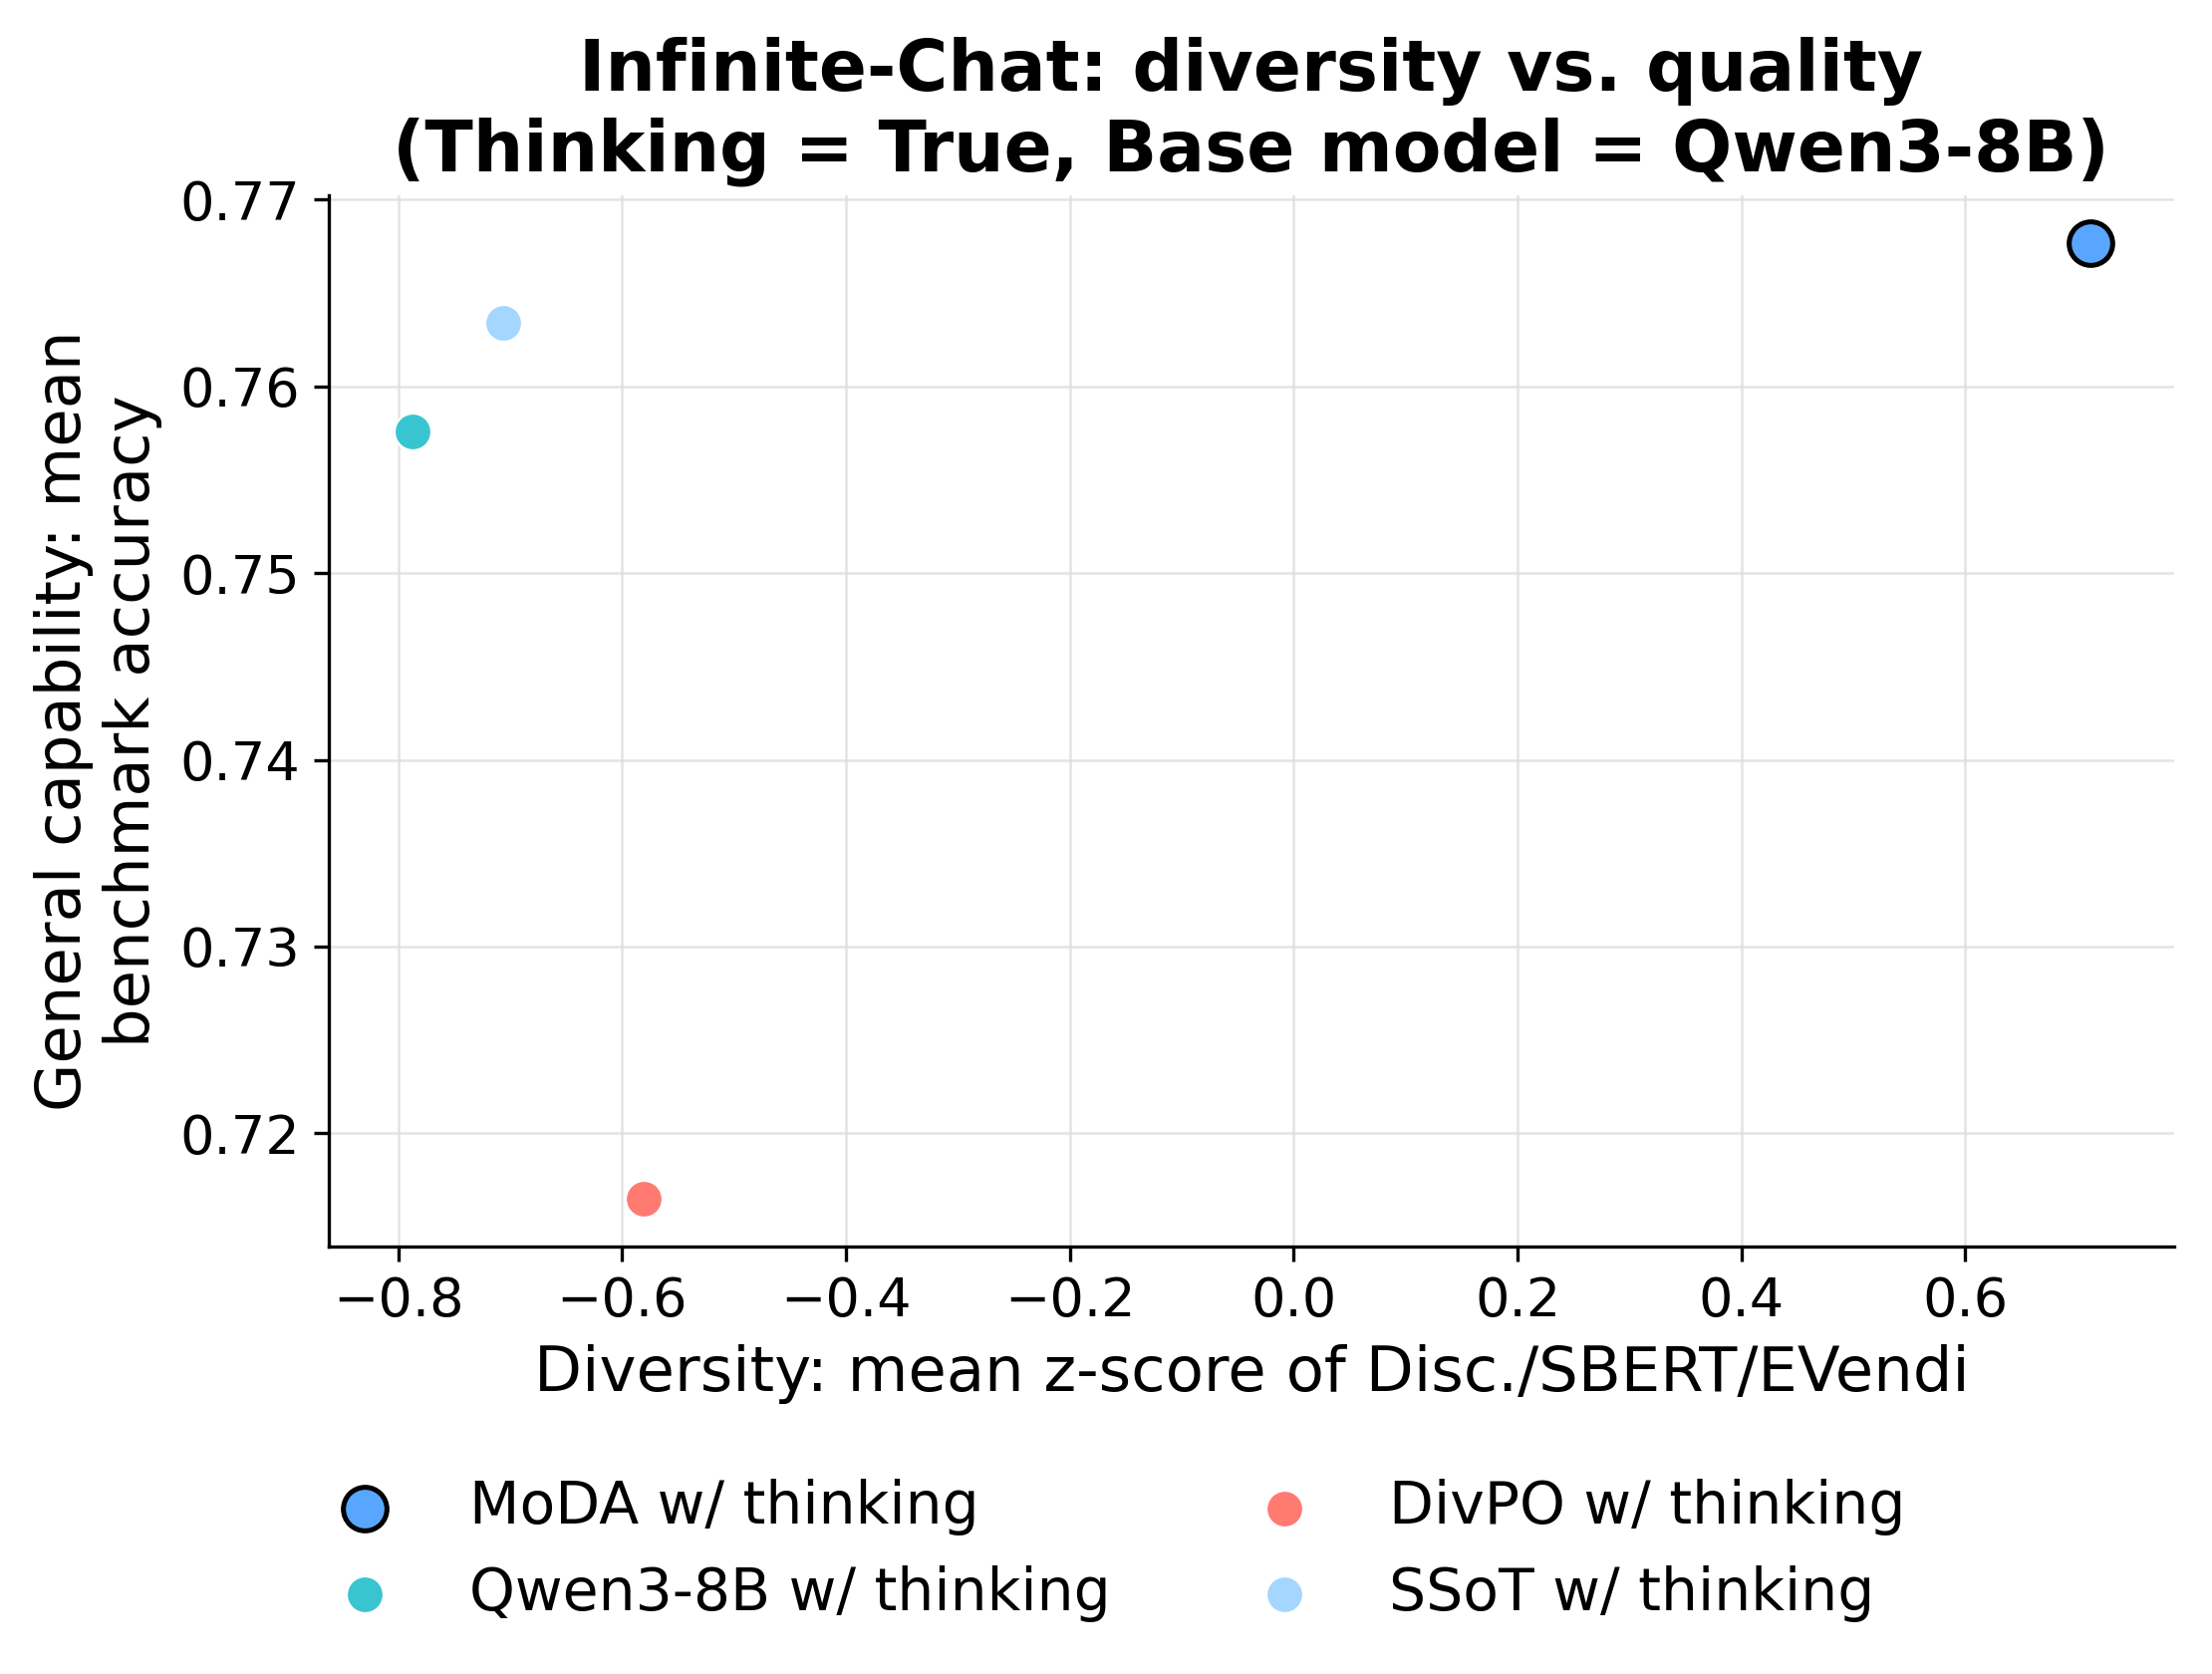
\includegraphics[width=\linewidth]{figures/pareto_infinite-chat_quality_thinking_true_base_model_qwen3-8b_composite.png}
\end{minipage}\hfill
\begin{minipage}{0.48\textwidth}
  \centering
  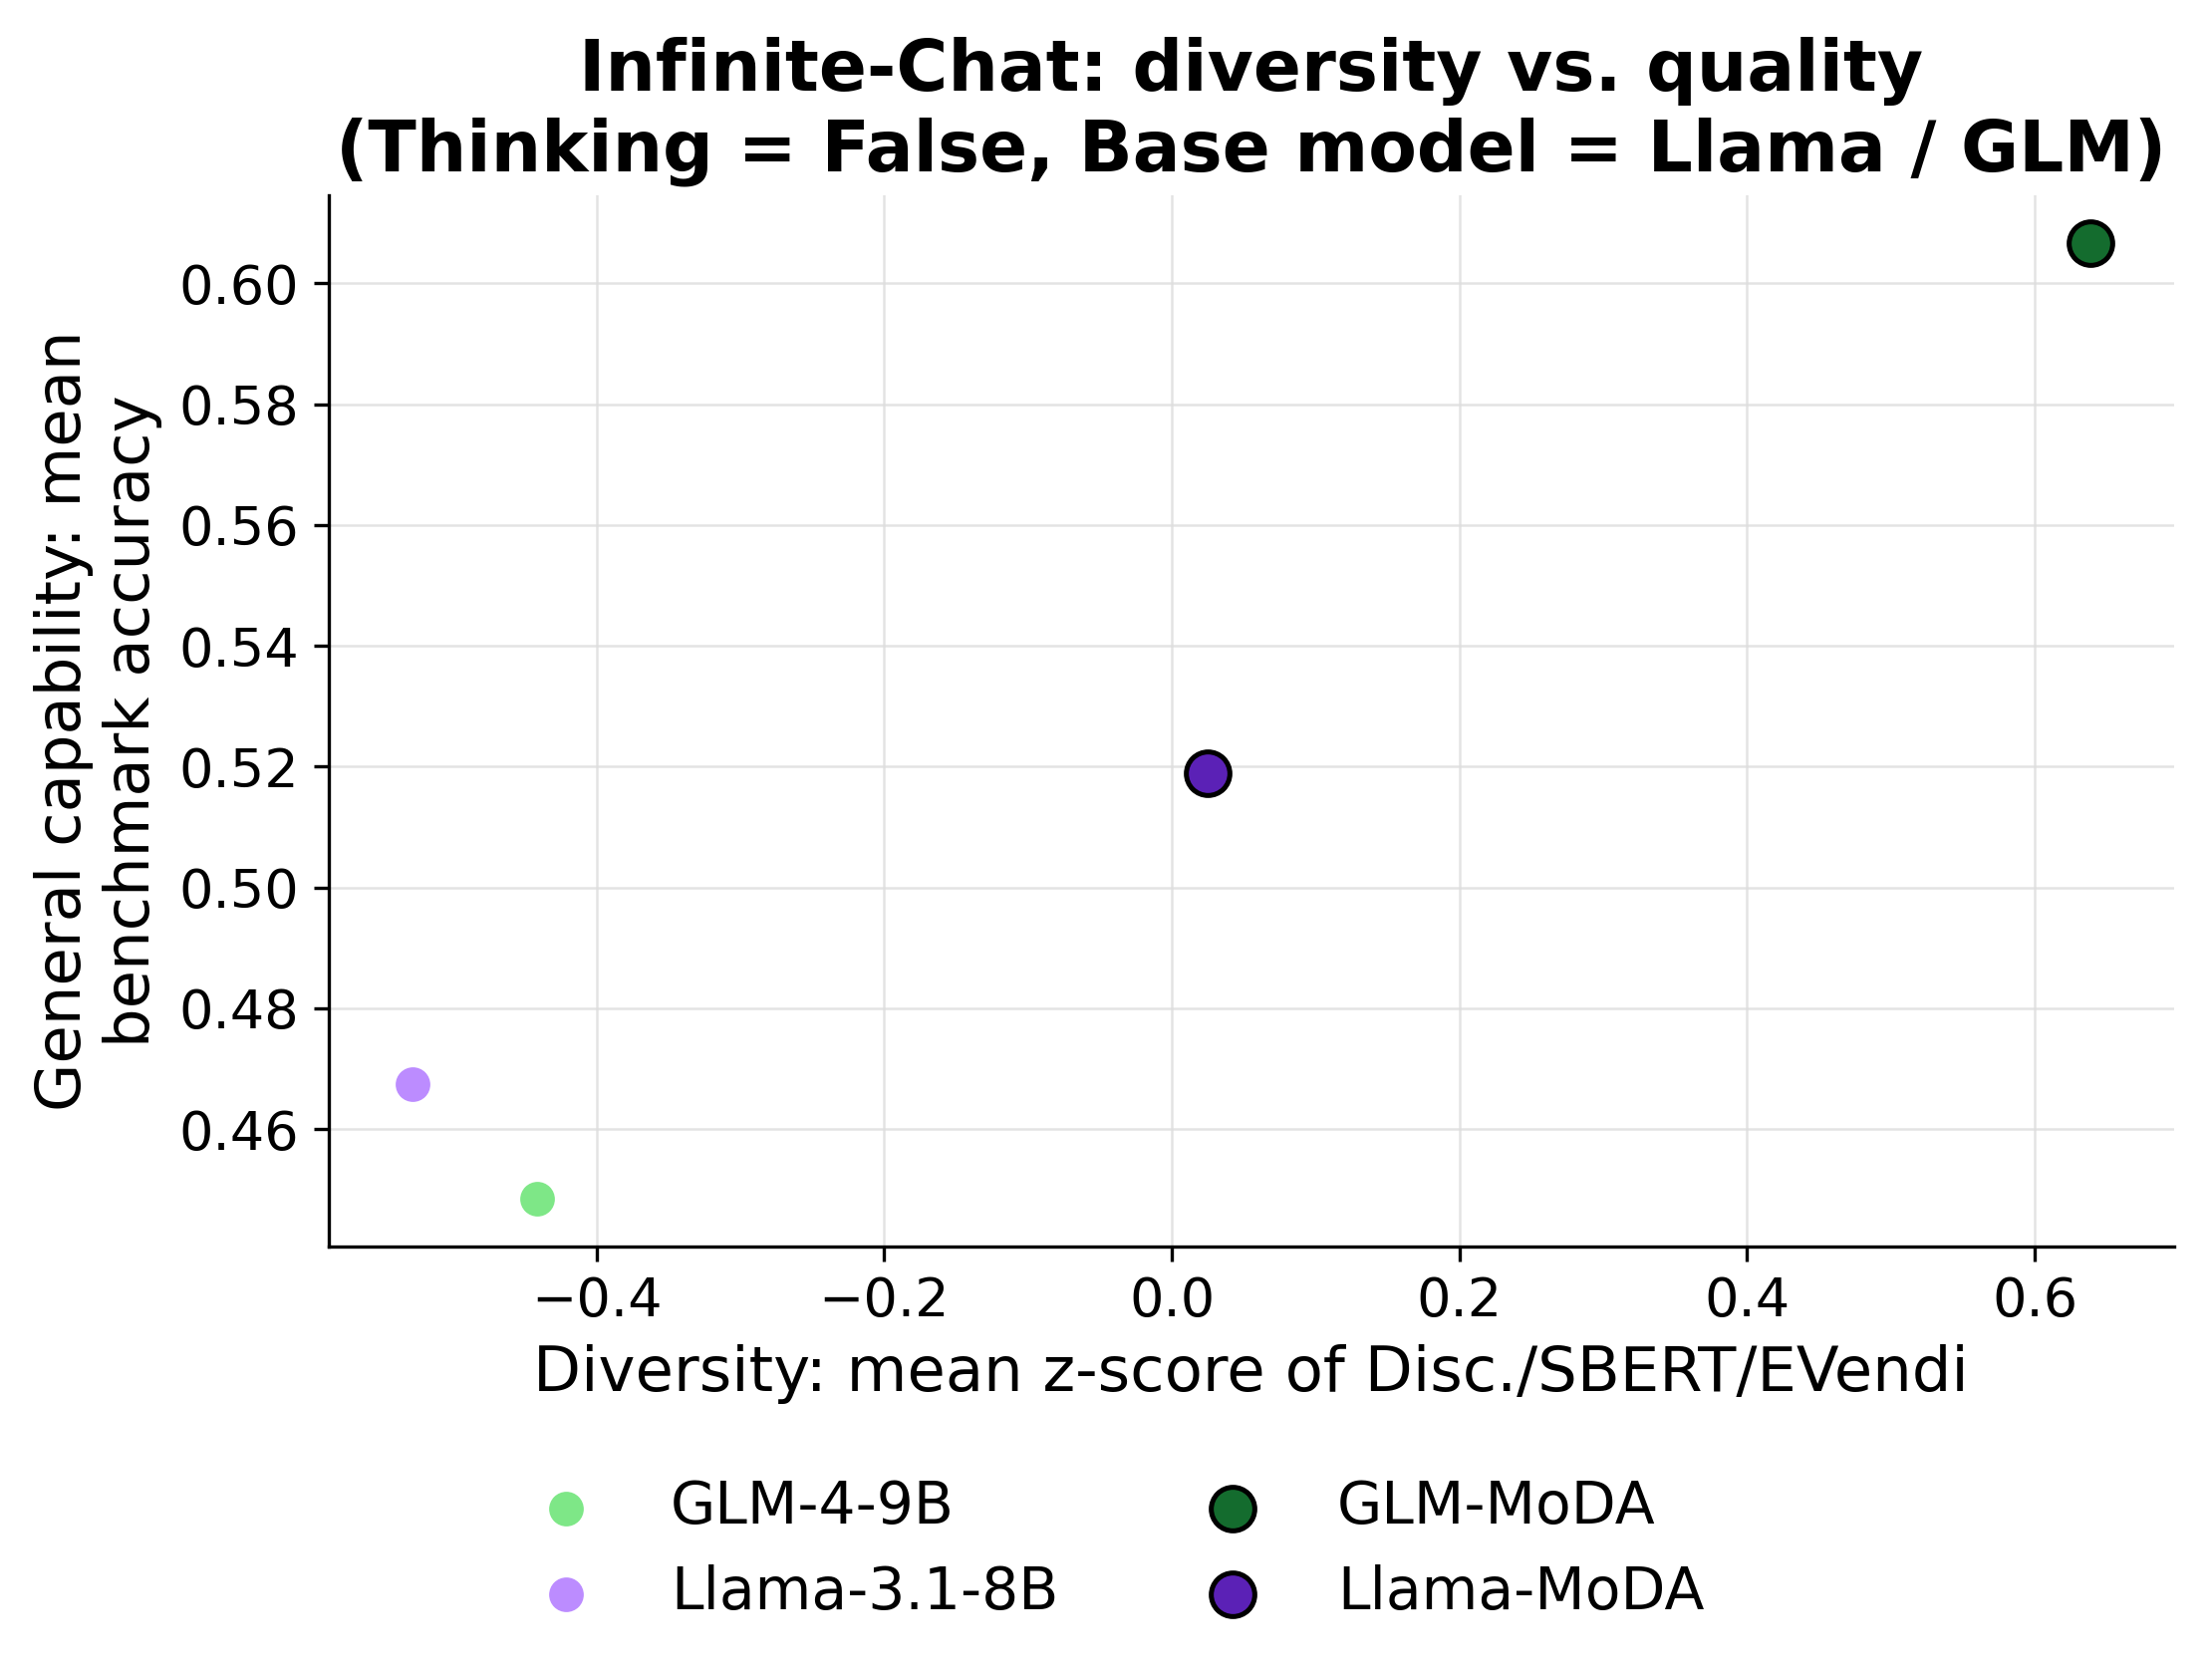
\includegraphics[width=\linewidth]{figures/pareto_infinite-chat_quality_thinking_false_base_model_llama_glm_composite.png}
\end{minipage}
\caption{\textbf{Diversity vs. quality pareto fronts, remaining settings} (extends Figure~\ref{fig: domain application pareto} in the main text). The x-axis is Infinite-Chat response diversity (mean z-score of Disc./SBERT/EmbVendi) and the y-axis is general capability (mean benchmark accuracy). \textbf{Left}: Qwen3-8B base, thinking enabled. \textbf{Right}: Llama-3.1-8B / GLM-4-9B base, thinking disabled. \method{} Pareto-dominates all baselines in both settings.}
\label{fig:domain-application-pareto-appendix}
\end{figure}

We show the results with error bar for generative diversity across all domain application tasks.


\section*{Infinite-Chat}

\begin{table}[H]
\centering
\begin{tabular}{lccccc}
\toprule
Model & Disc. & S & EV & Qual. \\
\midrule
\multicolumn{5}{l}{\textsc{\underline{Qwen3-8B base, thinking disabled}}} \\
Qwen3-8B & 0.400 $\pm$ 0.001 & 0.132 $\pm$ 0.001 & 1.83 $\pm$ 0.01 & 62.9\% $\pm$ 0.8\% \\
DARLING (Mix) & 0.430 $\pm$ 0.001 & 0.203 $\pm$ 0.001 & 2.33 $\pm$ 0.00 & 57.9\% $\pm$ 1.0\% \\
DARLING (WildChat) & 0.416 $\pm$ 0.001 & 0.185 $\pm$ 0.002 & 2.15 $\pm$ 0.01 & 62.7\% $\pm$ 1.0\% \\
DivPO & 0.410 $\pm$ 0.001 & 0.274 $\pm$ 0.004 & 2.86 $\pm$ 0.03 & 66.2\% $\pm$ 0.9\% \\
\method & \textbf{0.472} $\pm$ 0.001 & \textbf{0.482} $\pm$ 0.003 & \textbf{4.40} $\pm$ 0.01 & \textbf{73.2\%} $\pm$ 0.9\% \\
\midrule
\multicolumn{5}{l}{\textsc{\underline{Qwen3-8B base, thinking enabled}}} \\
Qwen3-8B & 0.400 $\pm$ 0.001 & 0.136 $\pm$ 0.001 & 1.85 $\pm$ 0.01 & 75.8\% $\pm$ 0.7\% \\
SSoT & 0.397 $\pm$ 0.000 & 0.178 $\pm$ 0.002 & 2.09 $\pm$ 0.01 & 76.3\% $\pm$ 0.7\% \\
DivPO & 0.414 $\pm$ 0.002 & 0.200 $\pm$ 0.006 & 2.20 $\pm$ 0.03 & 71.7\% $\pm$ 0.8\% \\
\method & \textbf{0.600} $\pm$ 0.001 & \textbf{0.909} $\pm$ 0.001 & \textbf{9.04} $\pm$ 0.01 & \textbf{76.8\%} $\pm$ 0.7\% \\
\midrule
\multicolumn{5}{l}{\textsc{\underline{Llama-3.1-8B base, thinking disabled}}} \\
Llama-3.1-8B & 0.414 $\pm$ 0.001 & 0.217 $\pm$ 0.002 & 2.40 $\pm$ 0.01 & 46.7\% $\pm$ 0.7\% \\
\method{} (Llama-3.1-8B) & \textbf{0.441} $\pm$ 0.002 & \textbf{0.373} $\pm$ 0.003 & \textbf{3.77} $\pm$ 0.02 & \textbf{51.9\%} $\pm$ 0.9\% \\
\midrule
\multicolumn{5}{l}{\textsc{\underline{GLM-4-9B base, thinking disabled}}} \\
GLM-4-9B & 0.421 $\pm$ 0.001 & 0.234 $\pm$ 0.002 & 2.60 $\pm$ 0.01 & 44.9\% $\pm$ 0.9\% \\
\method{}(GLM-4-9b) & \textbf{0.481} $\pm$ 0.001 & \textbf{0.528} $\pm$ 0.001 & \textbf{5.14} $\pm$ 0.01 & \textbf{60.7\%} $\pm$ 0.8\% \\
\bottomrule
\end{tabular}
\end{table}



\section*{NoveltyBench}

\begin{table}[H]
\centering
\begin{tabular}{lccccc}
\toprule
Model & Disc. & S & EV & Qual. \\
\midrule
\multicolumn{5}{l}{\textsc{\underline{Qwen3-8B base, thinking disabled}}} \\
Qwen3-8B & 0.493 $\pm$ 0.002 & 0.224 $\pm$ 0.003 & 2.36 $\pm$ 0.02 & 4.58 $\pm$ 0.04 \\
DARLING (Mix) & 0.513 $\pm$ 0.001 & 0.281 $\pm$ 0.001 & 2.96 $\pm$ 0.01 & 5.24 $\pm$ 0.07 \\
DARLING (WildChat) & 0.480 $\pm$ 0.001 & 0.335 $\pm$ 0.004 & 3.11 $\pm$ 0.02 & 4.00 $\pm$ 0.06 \\
DivPO & 0.519 $\pm$ 0.001 & 0.380 $\pm$ 0.003 & 3.58 $\pm$ 0.02 & 4.87 $\pm$ 0.02 \\
\method & \textbf{0.537} $\pm$ 0.001 & \textbf{0.470} $\pm$ 0.003 & \textbf{4.19} $\pm$ 0.01 & \textbf{5.47} $\pm$ 0.03 \\
\midrule
\multicolumn{5}{l}{\textsc{\underline{Qwen3-8B base, thinking enabled}}} \\
Qwen3-8B & 0.510 $\pm$ 0.001 & 0.258 $\pm$ 0.003 & 2.67 $\pm$ 0.03 & 4.90 $\pm$ 0.04 \\
SSoT & 0.438 $\pm$ 0.001 & 0.239 $\pm$ 0.002 & 2.57 $\pm$ 0.01 & 0.46 $\pm$ 0.01 \\
DivPO & 0.521 $\pm$ 0.001 & 0.327 $\pm$ 0.003 & 3.12 $\pm$ 0.02 & \textbf{5.06} $\pm$ 0.04 \\
\method & \textbf{0.589} $\pm$ 0.002 & \textbf{0.800} $\pm$ 0.004 & \textbf{7.63} $\pm$ 0.07 & 3.39 $\pm$ 0.05 \\
\midrule
\multicolumn{5}{l}{\textsc{\underline{Llama-3.1-8B base, thinking disabled}}} \\
Llama-3.1-8B & 0.512 $\pm$ 0.001 & 0.312 $\pm$ 0.001 & 3.04 $\pm$ 0.01 & 4.80 $\pm$ 0.08 \\
\method{} (Llama-3.1-8B) & \textbf{0.532} $\pm$ 0.001 & \textbf{0.392} $\pm$ 0.001 & \textbf{3.75} $\pm$ 0.01 & \textbf{6.17} $\pm$ 0.04 \\
\midrule
\multicolumn{5}{l}{\textsc{\underline{GLM-4-9B base, thinking disabled}}} \\
GLM-4-9B & \textbf{0.544} $\pm$ 0.002 & 0.408 $\pm$ 0.004 & 4.08 $\pm$ 0.04 & \textbf{4.14} $\pm$ 0.01 \\
\method{}(GLM-4-9b) & 0.502 $\pm$ 0.002 & \textbf{0.521} $\pm$ 0.005 & \textbf{5.01} $\pm$ 0.04 & 2.70 $\pm$ 0.03 \\
\bottomrule
\end{tabular}
\end{table}



\section*{HypoBench}

\begin{table}[H]
\centering
\begin{tabular}{lccccc}
\toprule
Model & Disc. & S & EV & Qual. \\
\midrule
\multicolumn{5}{l}{\textsc{\underline{Qwen3-8B base, thinking disabled}}} \\
Qwen3-8B & 0.384 $\pm$ 0.005 & 0.144 $\pm$ 0.005 & 1.91 $\pm$ 0.03 & \textbf{4.03} $\pm$ 0.01 \\
DARLING (Mix) & 0.406 $\pm$ 0.005 & 0.222 $\pm$ 0.004 & 2.48 $\pm$ 0.02 & 3.44 $\pm$ 0.03 \\
DARLING (WildChat) & 0.415 $\pm$ 0.004 & 0.205 $\pm$ 0.006 & 2.34 $\pm$ 0.04 & 3.73 $\pm$ 0.02 \\
DivPO & 0.427 $\pm$ 0.006 & 0.198 $\pm$ 0.005 & 2.30 $\pm$ 0.03 & 3.89 $\pm$ 0.01 \\
\method & \textbf{0.480} $\pm$ 0.003 & \textbf{0.547} $\pm$ 0.010 & \textbf{4.91} $\pm$ 0.05 & 3.80 $\pm$ 0.02 \\
\midrule
\multicolumn{5}{l}{\textsc{\underline{Qwen3-8B base, thinking enabled}}} \\
Qwen3-8B & 0.399 $\pm$ 0.006 & 0.164 $\pm$ 0.005 & 2.05 $\pm$ 0.03 & \textbf{3.93} $\pm$ 0.01 \\
SSoT & 0.419 $\pm$ 0.002 & 0.220 $\pm$ 0.010 & 2.33 $\pm$ 0.04 & 3.75 $\pm$ 0.02 \\
DivPO & 0.409 $\pm$ 0.002 & 0.162 $\pm$ 0.005 & 2.04 $\pm$ 0.03 & 3.89 $\pm$ 0.01 \\
\method & \textbf{0.579} $\pm$ 0.013 & \textbf{0.875} $\pm$ 0.018 & \textbf{8.06} $\pm$ 0.25 & 3.71 $\pm$ 0.04 \\
\midrule
\multicolumn{5}{l}{\textsc{\underline{Llama-3.1-8B base, thinking disabled}}} \\
Llama-3.1-8B & \textbf{0.469} $\pm$ 0.005 & 0.207 $\pm$ 0.006 & 2.38 $\pm$ 0.04 & 3.60 $\pm$ 0.02 \\
\method{} (Llama-3.1-8B) & 0.410 $\pm$ 0.001 & \textbf{0.324} $\pm$ 0.014 & \textbf{3.27} $\pm$ 0.10 & \textbf{3.65} $\pm$ 0.01 \\
\midrule
\multicolumn{5}{l}{\textsc{\underline{GLM-4-9B base, thinking disabled}}} \\
GLM-4-9B & 0.402 $\pm$ 0.003 & 0.225 $\pm$ 0.005 & 2.52 $\pm$ 0.03 & \textbf{3.75} $\pm$ 0.01 \\
\method{}(GLM-4-9b) & \textbf{0.452} $\pm$ 0.003 & \textbf{0.485} $\pm$ 0.012 & \textbf{4.64} $\pm$ 0.09 & 3.68 $\pm$ 0.01 \\
\bottomrule
\end{tabular}
\end{table}


\section*{PreScience}

\begin{table}[H]
\centering
\begin{tabular}{lccccc}
\toprule
Model & Disc. & S & EV & Qual. \\
\midrule
\multicolumn{5}{l}{\textsc{\underline{Qwen3-8B base, thinking disabled}}} \\
Qwen3-8B & 0.431 $\pm$ 0.002 & 0.155 $\pm$ 0.004 & 1.94 $\pm$ 0.02 & \textbf{4.25} $\pm$ 0.03 \\
DARLING (Mix) & \textbf{0.559} $\pm$ 0.005 & \textbf{0.541} $\pm$ 0.018 & \textbf{4.73} $\pm$ 0.15 & 2.33 $\pm$ 0.07 \\
DARLING (WildChat) & 0.446 $\pm$ 0.002 & 0.192 $\pm$ 0.003 & 2.21 $\pm$ 0.03 & 4.03 $\pm$ 0.06 \\
DivPO & 0.455 $\pm$ 0.002 & 0.233 $\pm$ 0.001 & 2.41 $\pm$ 0.01 & 3.96 $\pm$ 0.05 \\
\method & 0.440 $\pm$ 0.002 & 0.176 $\pm$ 0.002 & 2.10 $\pm$ 0.01 & 3.96 $\pm$ 0.01 \\
\midrule
\multicolumn{5}{l}{\textsc{\underline{Qwen3-8B base, thinking enabled}}} \\
Qwen3-8B & 0.441 $\pm$ 0.003 & 0.136 $\pm$ 0.001 & 1.83 $\pm$ 0.01 & 3.79 $\pm$ 0.04 \\
SSoT & \textbf{0.461} $\pm$ 0.002 & \textbf{0.281} $\pm$ 0.017 & \textbf{2.39} $\pm$ 0.05 & 3.30 $\pm$ 0.05 \\
DivPO & 0.448 $\pm$ 0.003 & 0.185 $\pm$ 0.015 & 2.04 $\pm$ 0.07 & \textbf{3.87} $\pm$ 0.06 \\
\method & 0.439 $\pm$ 0.001 & 0.194 $\pm$ 0.005 & 2.10 $\pm$ 0.01 & 3.68 $\pm$ 0.00 \\
\midrule
\multicolumn{5}{l}{\textsc{\underline{Llama-3.1-8B base, thinking disabled}}} \\
Llama-3.1-8B & 0.461 $\pm$ 0.005 & \textbf{0.514} $\pm$ 0.020 & 3.67 $\pm$ 0.07 & \textbf{2.62} $\pm$ 0.05 \\
\method{} (Llama-3.1-8B) & \textbf{0.472} $\pm$ 0.003 & 0.470 $\pm$ 0.009 & \textbf{3.89} $\pm$ 0.07 & 2.54 $\pm$ 0.04 \\
\midrule
\multicolumn{5}{l}{\textsc{\underline{GLM-4-9B base, thinking disabled}}} \\
GLM-4-9B & 0.461 $\pm$ 0.004 & 0.438 $\pm$ 0.010 & 4.15 $\pm$ 0.08 & 2.57 $\pm$ 0.05 \\
\method{}(GLM-4-9b) & \textbf{0.464} $\pm$ 0.002 & \textbf{0.448} $\pm$ 0.010 & \textbf{4.28} $\pm$ 0.09 & \textbf{2.58} $\pm$ 0.10 \\
\bottomrule
\end{tabular}
\end{table}

\subsection{General Capability Retention}
\label{appx:general capability retention}

\subsubsection{Pass@1}
We show general capability retention with error bar for pass@1 across baselines and our model.
\begin{table}[H]
\setlength{\tabcolsep}{2.5pt}
\centering
\small
\begin{tabular}{lcccccccc}
\toprule
Model & GSM8K & MMLU & GPQA & BoolQ & HellaSwag & TruthfulQA & IFEval & Avg. \\
\midrule
\multicolumn{9}{l}{\textsc{\underline{Qwen3-8B base, thinking disabled}}} \\
Qwen3-8B & 84.5 $\pm$ 1.0 & \textbf{82.0} $\pm$ 3.9 & 41.4 $\pm$ 3.5 & 83.1 $\pm$ 0.7 & 48.4 $\pm$ 0.5 & 22.2 $\pm$ 1.5 & \textbf{78.4} $\pm$ 1.8 & 62.9 $\pm$ 0.8 \\
DARLING (Mixture) & 63.5 $\pm$ 1.3 & 63.0 $\pm$ 4.9 & 34.3 $\pm$ 3.4 & 76.7 $\pm$ 0.7 & 62.2 $\pm$ 0.5 & 52.4 $\pm$ 1.7 & 53.0 $\pm$ 2.1 & 57.9 $\pm$ 1.0 \\
DARLING (WildChat) & 77.9 $\pm$ 1.1 & 55.0 $\pm$ 5.0 & 34.3 $\pm$ 3.4 & \textbf{86.4} $\pm$ 0.6 & 68.8 $\pm$ 0.5 & 43.2 $\pm$ 1.7 & 73.0 $\pm$ 1.9 & 62.7 $\pm$ 1.0 \\
DivPO & 80.5 $\pm$ 1.1 & 81.0 $\pm$ 3.9 & 40.4 $\pm$ 3.5 & 83.5 $\pm$ 0.6 & 62.8 $\pm$ 0.5 & 37.7 $\pm$ 1.7 & 77.3 $\pm$ 1.8 & 66.2 $\pm$ 0.9 \\
\method & \textbf{86.7} $\pm$ 0.9 & 81.0 $\pm$ 3.9 & \textbf{52.0} $\pm$ 3.6 & 84.8 $\pm$ 0.6 & \textbf{73.4} $\pm$ 0.4 & \textbf{57.9} $\pm$ 1.7 & 76.9 $\pm$ 1.8 & \textbf{73.2} $\pm$ 0.9 \\
\midrule
\multicolumn{9}{l}{\textsc{\underline{Qwen3-8B base, thinking enabled}}} \\
Qwen3-8B & \textbf{90.3} $\pm$ 0.8 & \textbf{94.0} $\pm$ 2.4 & 43.4 $\pm$ 3.5 & \textbf{87.2} $\pm$ 0.6 & 70.9 $\pm$ 0.5 & 64.9 $\pm$ 1.7 & \textbf{79.7} $\pm$ 1.7 & 75.8 $\pm$ 0.7 \\
SSoT & 84.3 $\pm$ 1.0 & 93.0 $\pm$ 2.6 & \textbf{55.1} $\pm$ 3.5 & \textbf{87.2} $\pm$ 0.6 & \textbf{80.1} $\pm$ 0.4 & \textbf{72.8} $\pm$ 1.6 & 61.9 $\pm$ 2.1 & 76.3 $\pm$ 0.7 \\
DivPO & 84.9 $\pm$ 1.0 & 91.0 $\pm$ 2.9 & 44.4 $\pm$ 3.5 & 83.2 $\pm$ 0.7 & 65.0 $\pm$ 0.5 & 55.3 $\pm$ 1.7 & 77.6 $\pm$ 1.8 & 71.7 $\pm$ 0.8 \\
\method & 83.9 $\pm$ 1.0 & 93.0 $\pm$ 2.6 & 50.5 $\pm$ 3.6 & \textbf{87.2} $\pm$ 0.6 & 76.2 $\pm$ 0.4 & 67.2 $\pm$ 1.6 & 79.5 $\pm$ 1.7 & \textbf{76.8} $\pm$ 0.7 \\
\midrule
\multicolumn{9}{l}{\textsc{\underline{Llama-3.1-8B base, thinking disabled}}} \\
Llama-3.1-8B & 71.3 $\pm$ 1.2 & 16.0 $\pm$ 3.7 & 6.1 $\pm$ 1.7 & \textbf{81.6} $\pm$ 0.7 & 30.2 $\pm$ 0.5 & 53.4 $\pm$ 1.7 & 68.8 $\pm$ 2.0 & 46.7 $\pm$ 0.7 \\
\method(Llama-3.1-8B) & \textbf{74.9} $\pm$ 1.2 & \textbf{30.0} $\pm$ 4.6 & \textbf{18.7} $\pm$ 2.8 & 75.6 $\pm$ 0.8 & \textbf{38.5} $\pm$ 0.5 & \textbf{54.7} $\pm$ 1.7 & \textbf{70.8} $\pm$ 2.0 & \textbf{51.9} $\pm$ 0.9 \\
\midrule
\multicolumn{9}{l}{\textsc{\underline{GLM-4-9B base, thinking disabled}}} \\
GLM-4-9B & 21.8 $\pm$ 1.1 & 35.0 $\pm$ 4.8 & 19.7 $\pm$ 2.8 & 74.5 $\pm$ 0.8 & \textbf{68.0} $\pm$ 0.5 & \textbf{44.8} $\pm$ 1.7 & 50.3 $\pm$ 2.2 & 44.9 $\pm$ 0.9 \\
\method(GLM-4-9B) & \textbf{84.9} $\pm$ 1.0 & \textbf{83.0} $\pm$ 3.8 & \textbf{33.3} $\pm$ 3.4 & \textbf{81.2} $\pm$ 0.7 & 52.3 $\pm$ 0.5 & 34.5 $\pm$ 1.7 & \textbf{55.5} $\pm$ 2.1 & \textbf{60.7} $\pm$ 0.8 \\
\bottomrule
\end{tabular}
\vspace{4pt}
\caption{General capability retention (accuracy \%, mean ± std error; bold = best per block)}
\label{tab:general-capability-pass1-error-bar}
\end{table}

\subsubsection{Pass@5}
We show general capability retention for pass@5 across baselines and our model.
\begin{table}[H]
\centering
\small
\setlength{\tabcolsep}{4pt}
\resizebox{\textwidth}{!}{%
\begin{tabular}{lcccccccc}
\toprule
Model & GSM8K & MMLU & GPQA & BoolQ & HellaSwag & TruthfulQA & IFEval & Avg. \\
\midrule
\multicolumn{9}{l}{\textsc{\underline{Qwen3-8B base, thinking disabled}}} \\
Qwen3-8B & 92.6 & 92.0 & 73.7 & 89.7 & 86.0 & 55.1 & 83.4 & 81.8 \\
DARLING (Mixture) & 92.8 & \textbf{95.0} & \textbf{75.3} & 93.1 & 91.2 & 86.4 & 57.3 & 84.4 \\
DARLING (WildChat) & 91.8 & 86.0 & 69.2 & 91.3 & 91.3 & 74.4 & 80.8 & 83.5 \\
DivPO & 92.3 & 92.0 & 74.7 & 93.2 & 90.5 & 76.3 & \textbf{85.6} & 86.4 \\
\method & \textbf{94.5} & 93.0 & 74.7 & \textbf{93.9} & \textbf{91.3} & \textbf{86.5} & 83.9 & \textbf{88.3} \\
\midrule
\multicolumn{9}{l}{\textsc{\underline{Qwen3-8B base, thinking enabled}}} \\
Qwen3-8B & 96.1 & 96.0 & 66.2 & 92.2 & 89.1 & 82.5 & 85.4 & 86.8 \\
SSoT & 90.6 & 96.0 & \textbf{74.7} & 92.0 & 88.9 & \textbf{83.8} & 73.6 & 85.7 \\
DivPO & 94.0 & \textbf{97.0} & 72.2 & \textbf{93.0} & \textbf{89.8} & \textbf{83.8} & 85.6 & \textbf{87.9} \\
\method & \textbf{96.3} & 96.0 & 68.7 & 92.0 & 89.6 & 82.5 & \textbf{85.8} & 87.3 \\
\midrule
\multicolumn{9}{l}{\textsc{\underline{Llama-3.1-8B base, thinking disabled}}} \\
Llama-3.1-8B & 90.1 & 57.0 & 28.3 & \textbf{93.2} & 70.2 & 72.9 & \textbf{82.3} & 70.6 \\
\method(Llama-3.1-8B) & \textbf{93.5} & \textbf{76.0} & \textbf{56.6} & 92.3 & \textbf{79.6} & \textbf{80.4} & 80.2 & \textbf{79.8} \\
\midrule
\multicolumn{9}{l}{\textsc{\underline{GLM-4-9b base, thinking disabled}}} \\
GLM-4-9B & 60.0 & 69.0 & 59.6 & \textbf{97.1} & \textbf{91.3} & \textbf{82.6} & 57.5 & 73.9 \\
\method(GLM-4-9B) & \textbf{95.2} & \textbf{94.0} & \textbf{73.2} & 95.3 & 89.1 & 77.5 & \textbf{74.7} & \textbf{85.6} \\
\bottomrule
\end{tabular}
}
\vspace{4pt}
\caption{General capability retention pass@5. For IFEval, strict instruction-following accuracy is reported. Avg.\ is the row mean across benchmarks. Bold marks the best average within each thinking setting.}
\label{tab:general-capability-pass5}
\end{table}


We show pass@k figures for the rest of the general capability suite tasks below.
\begin{figure}[H]
\centering
\begin{minipage}{0.24\textwidth}
  \centering
  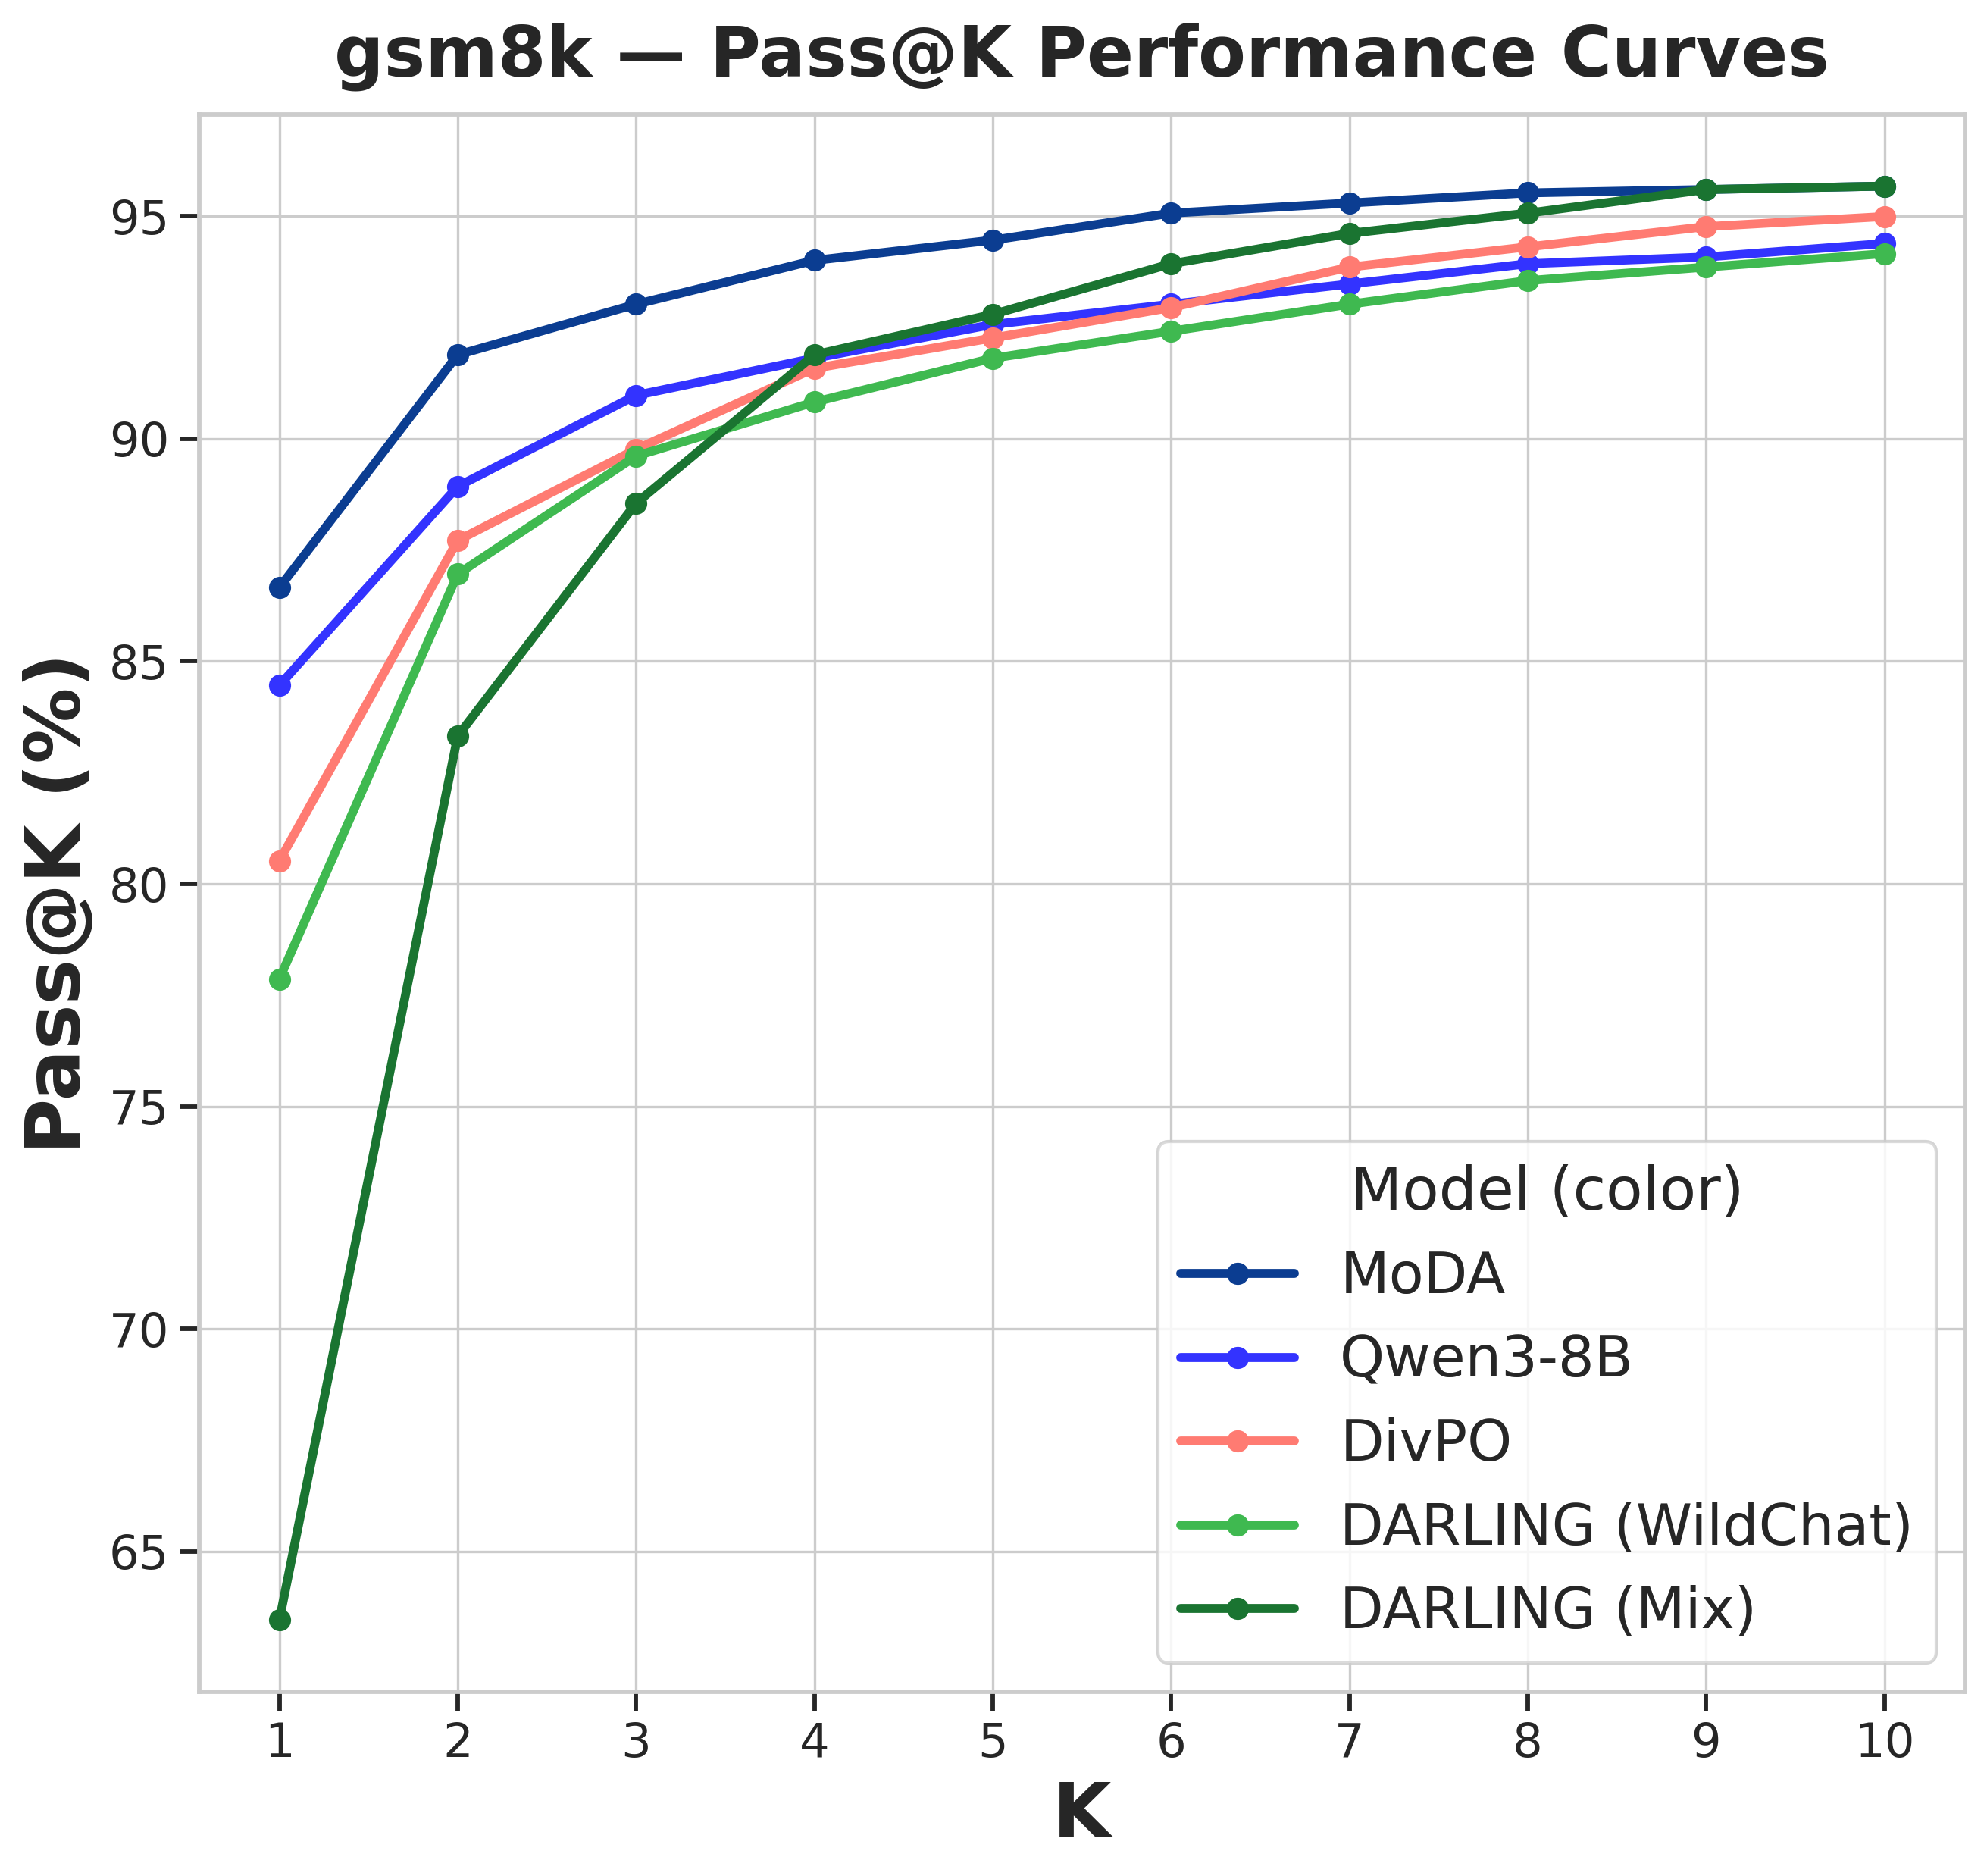
\includegraphics[width=\linewidth]{figures/main_pass_k/pass_at_k_figures/pass_at_k_gsm8k_thinking_false_base_model_qwen3-8b.png}
\end{minipage}\hfill
\begin{minipage}{0.24\textwidth}
  \centering
  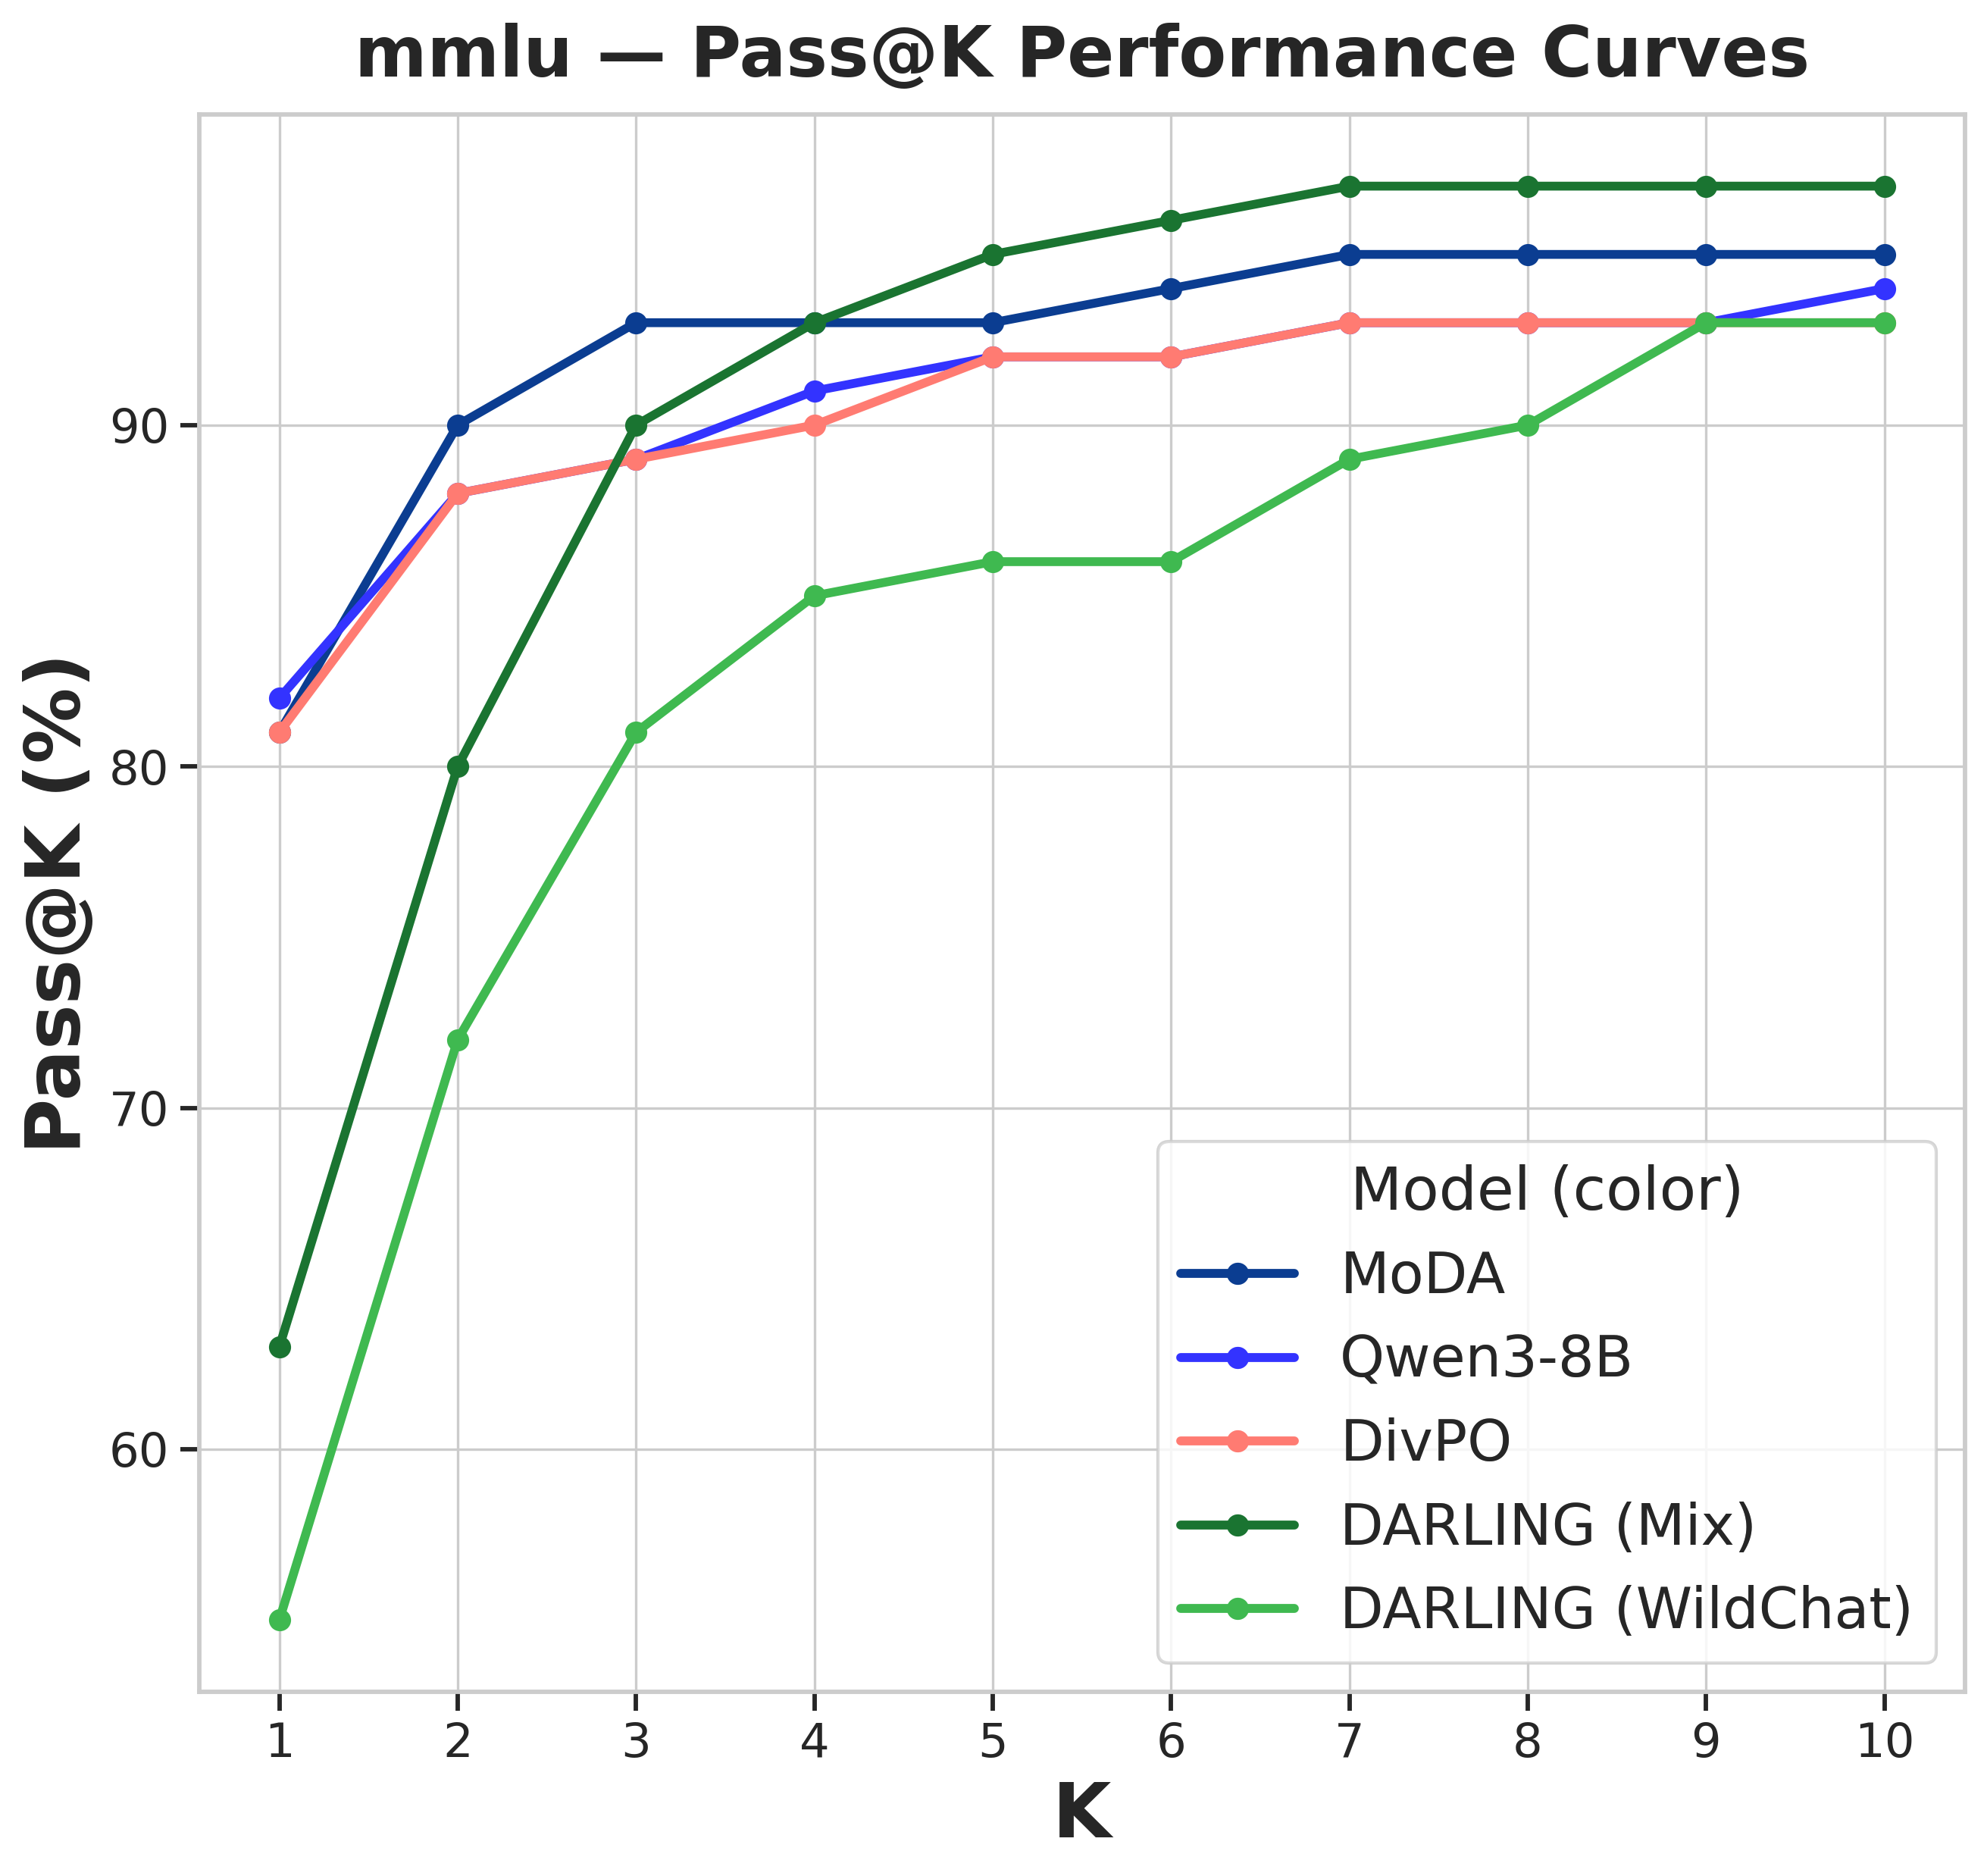
\includegraphics[width=\linewidth]{figures/main_pass_k/pass_at_k_figures/pass_at_k_mmlu_thinking_false_base_model_qwen3-8b.png}
\end{minipage}\hfill
\begin{minipage}{0.24\textwidth}
  \centering
  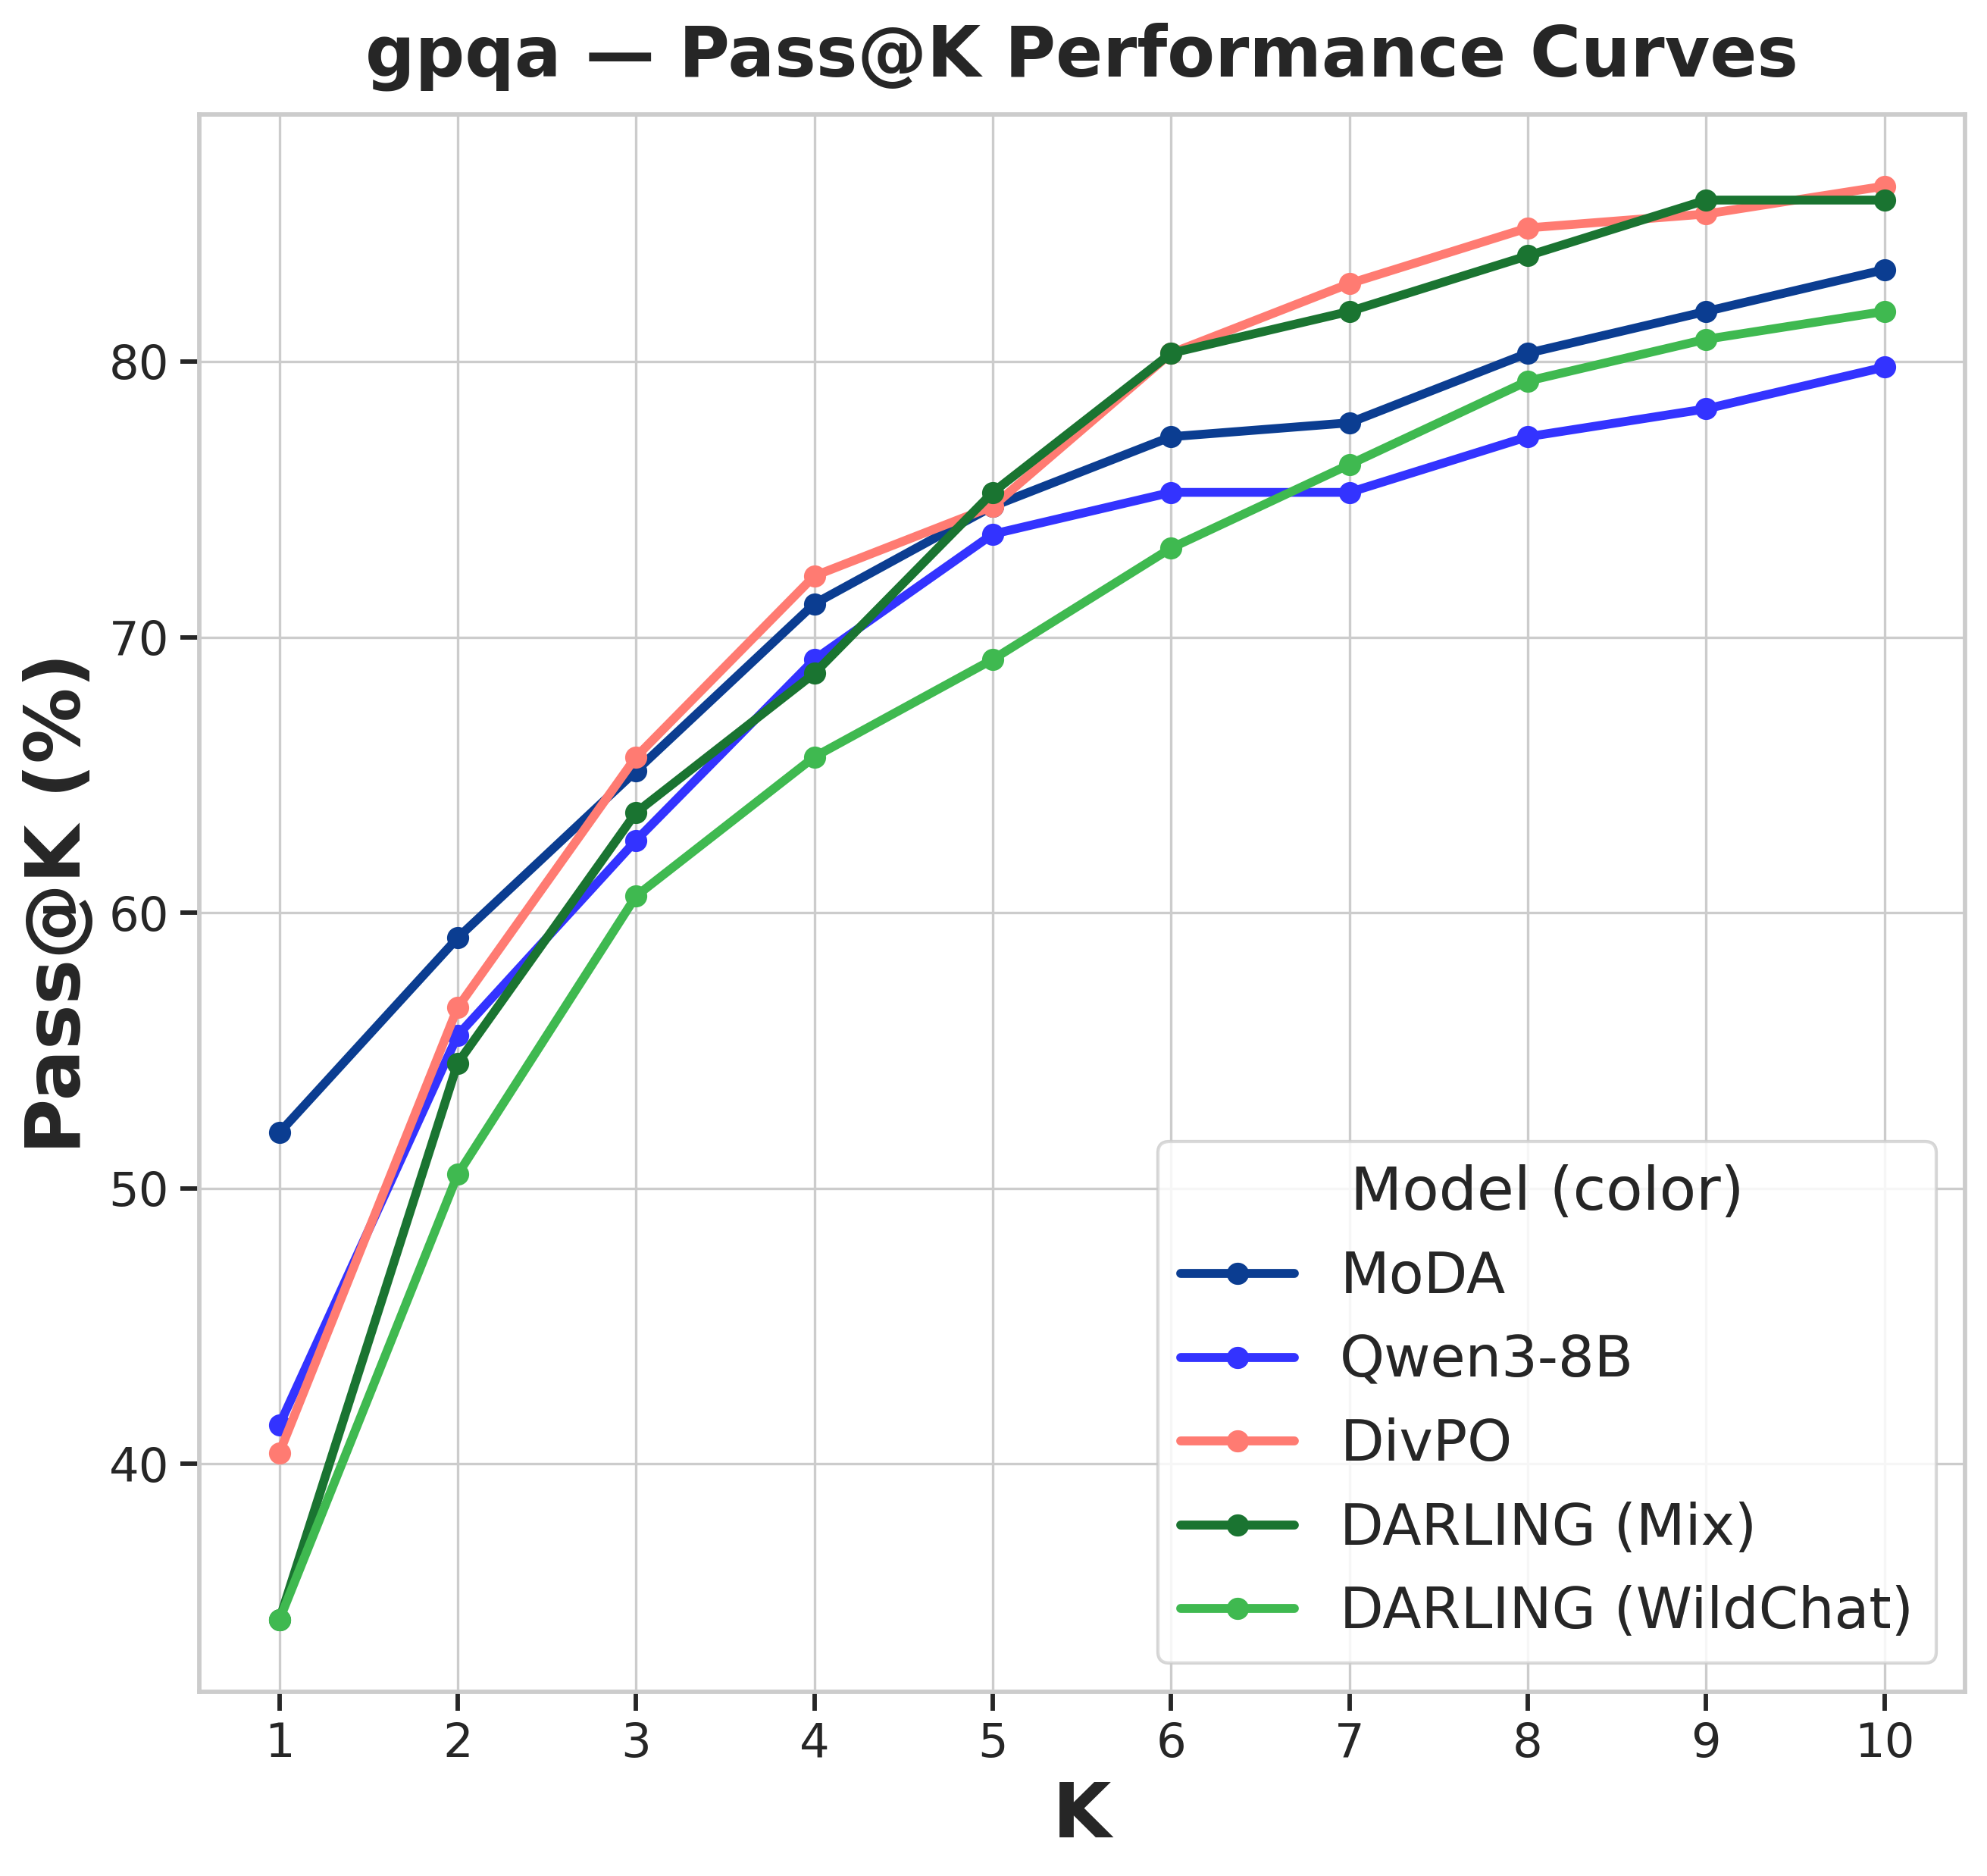
\includegraphics[width=\linewidth]{figures/main_pass_k/pass_at_k_figures/pass_at_k_gpqa_thinking_false_base_model_qwen3-8b.png}
\end{minipage}\hfill
\begin{minipage}{0.24\textwidth}
  \centering
  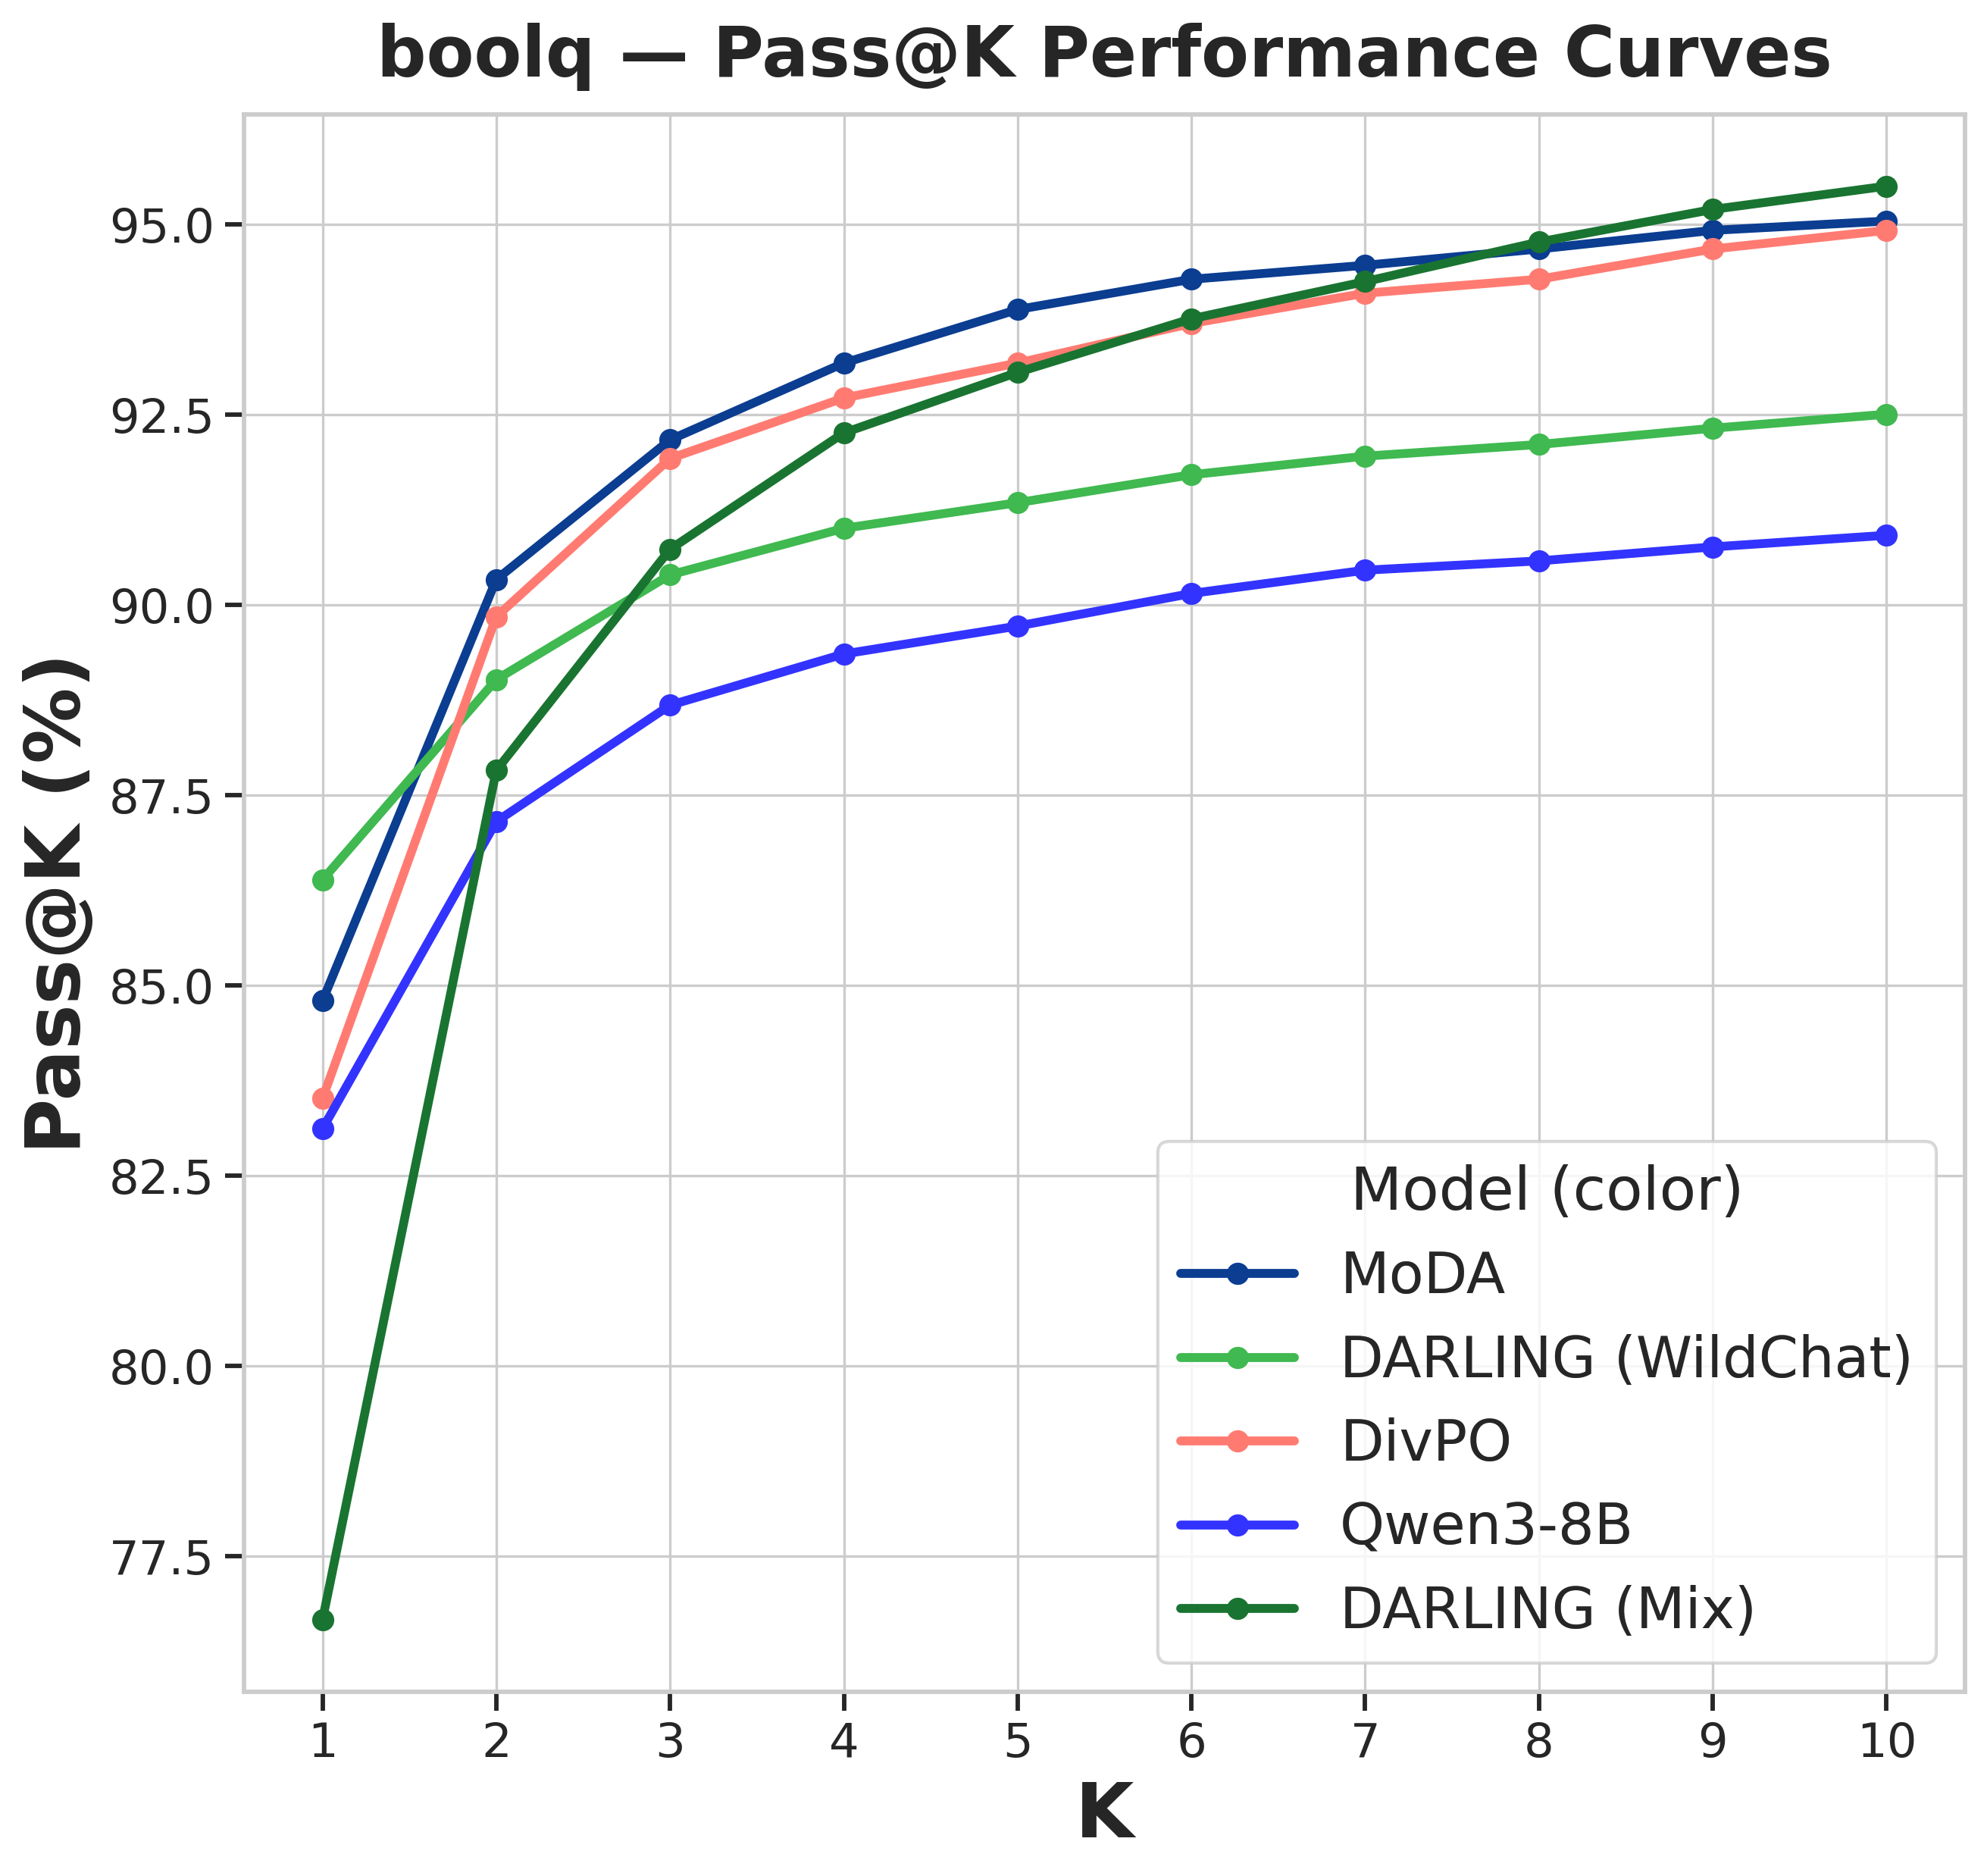
\includegraphics[width=\linewidth]{figures/main_pass_k/pass_at_k_figures/pass_at_k_boolq_thinking_false_base_model_qwen3-8b.png}
\end{minipage}

\vspace{4pt}
\begin{minipage}{0.24\textwidth}
  \centering
  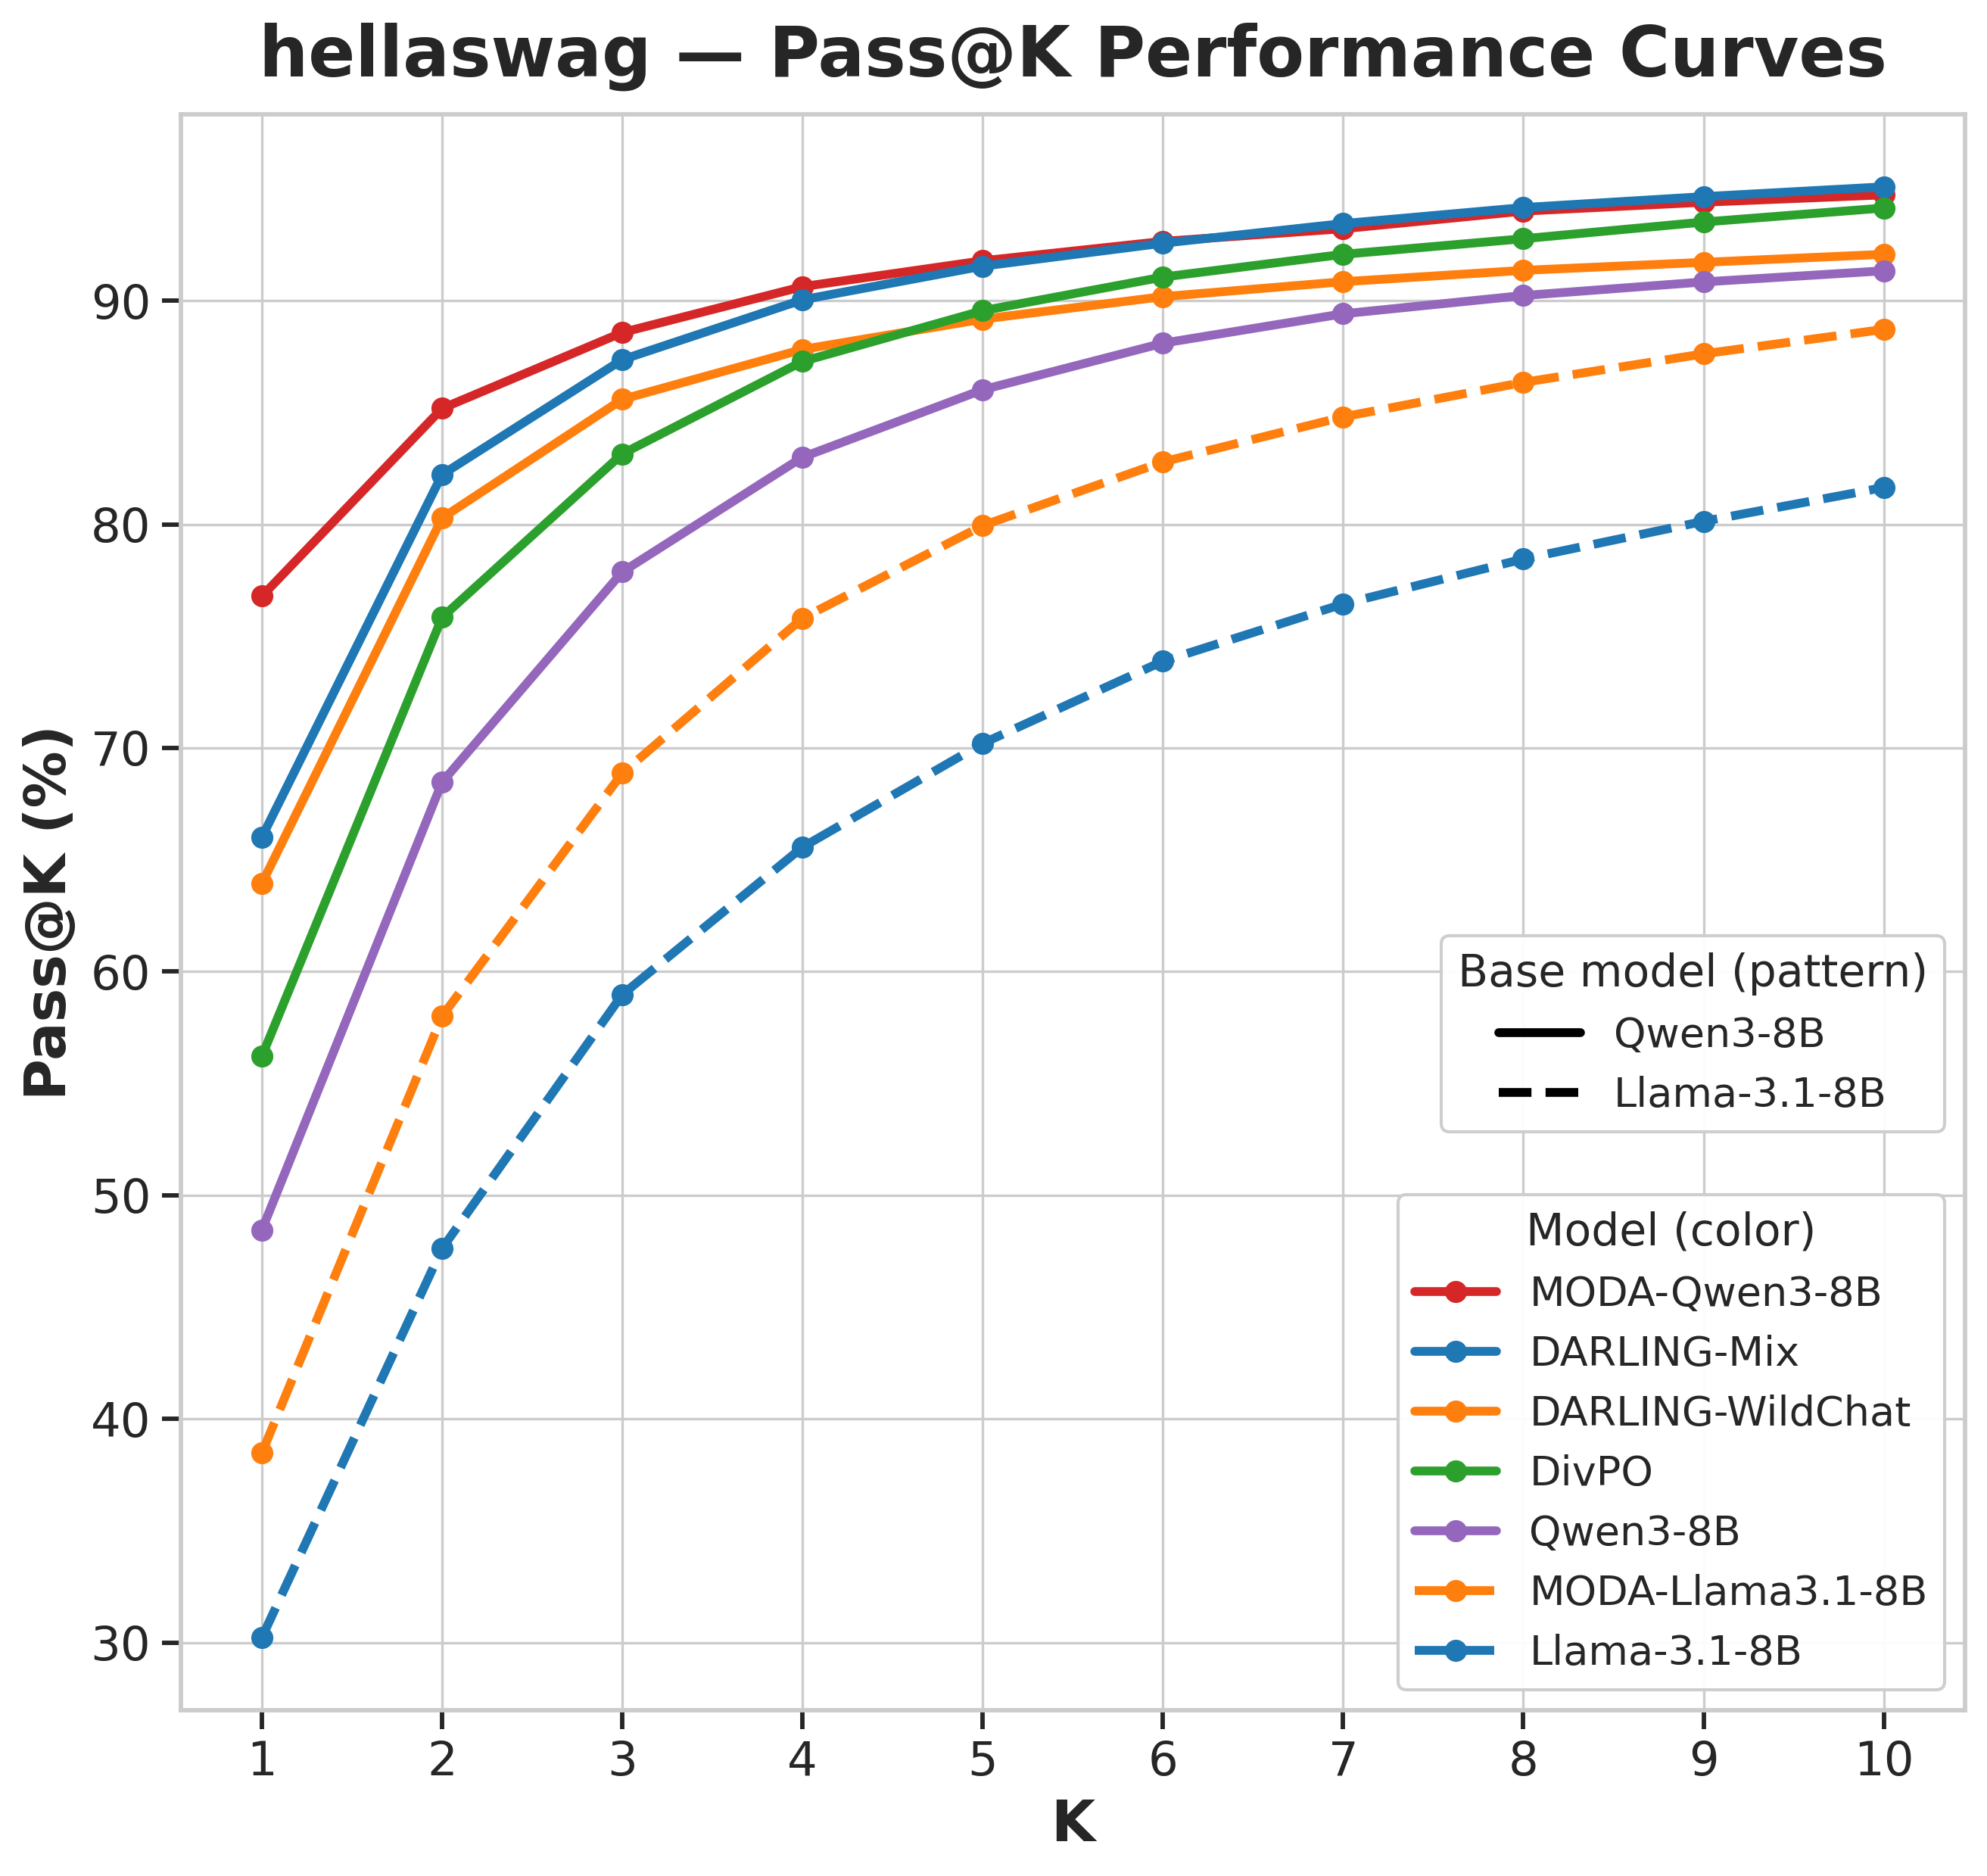
\includegraphics[width=\linewidth]{figures/main_pass_k/pass_at_k_curves_hellaswag.png}
\end{minipage}\hfill
\begin{minipage}{0.24\textwidth}
  \centering
  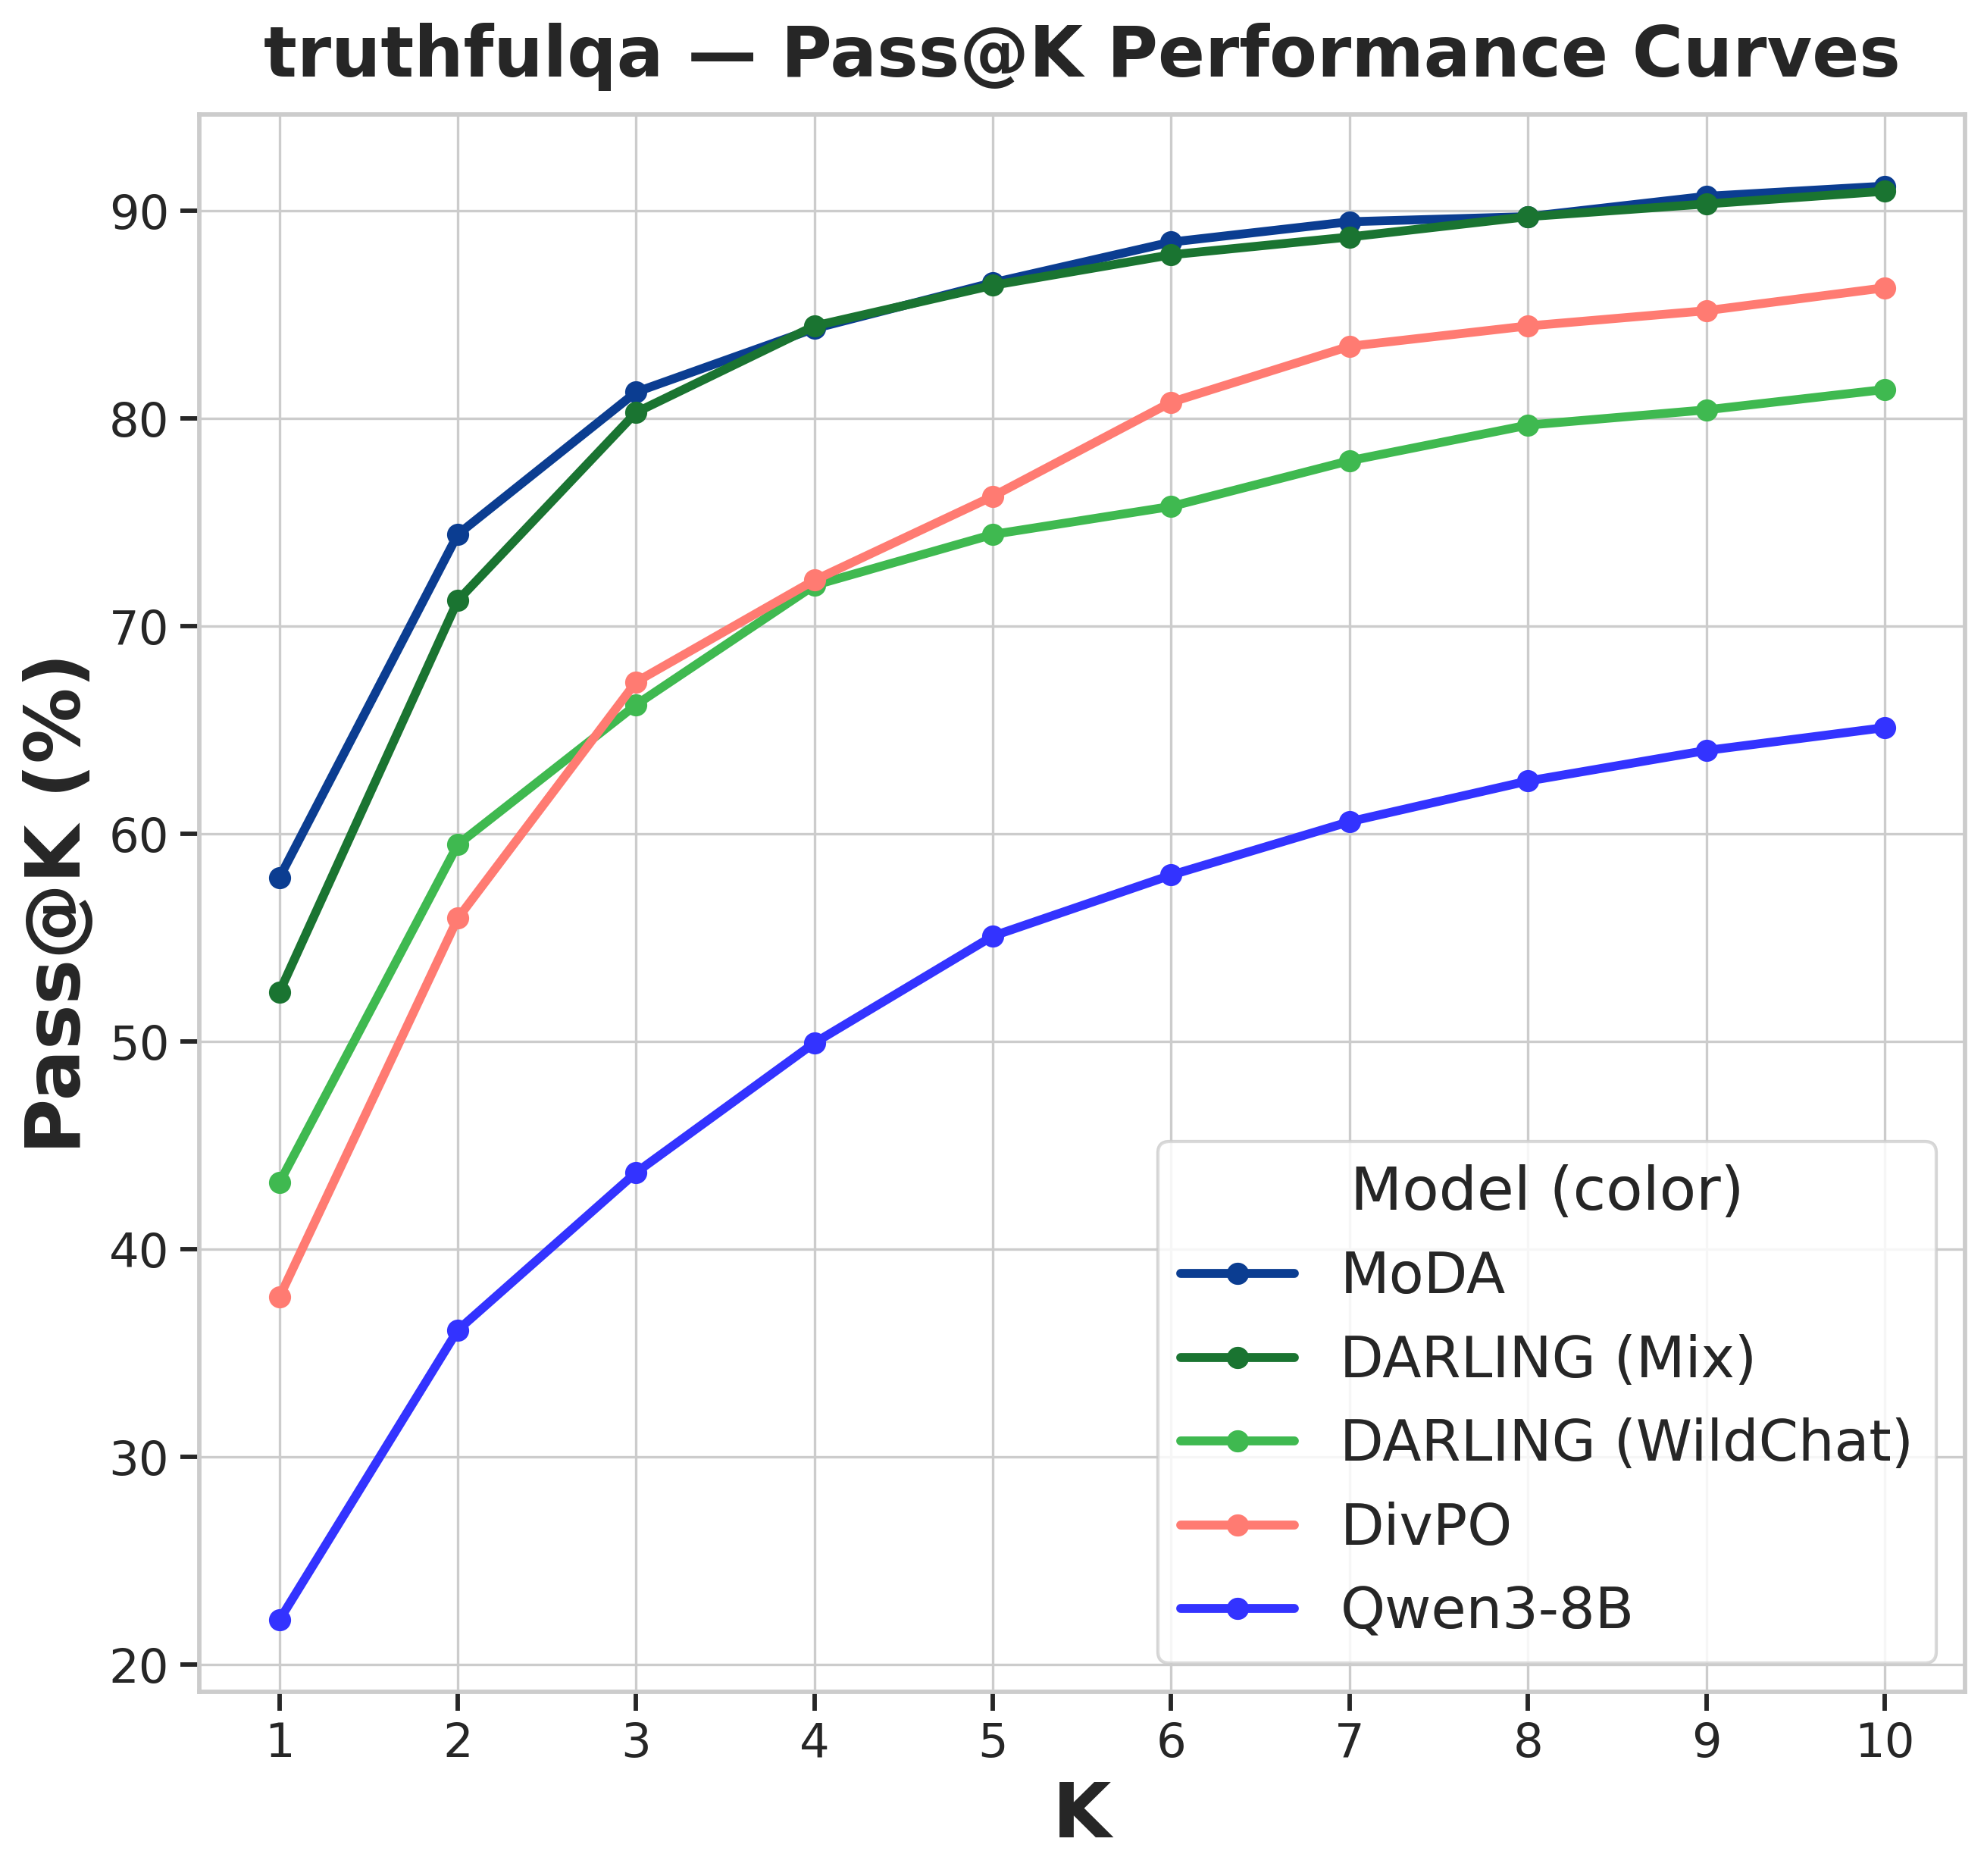
\includegraphics[width=\linewidth]{figures/main_pass_k/pass_at_k_figures/pass_at_k_truthfulqa_thinking_false_base_model_qwen3-8b.png}
\end{minipage}\hfill
\begin{minipage}{0.24\textwidth}
  \centering
  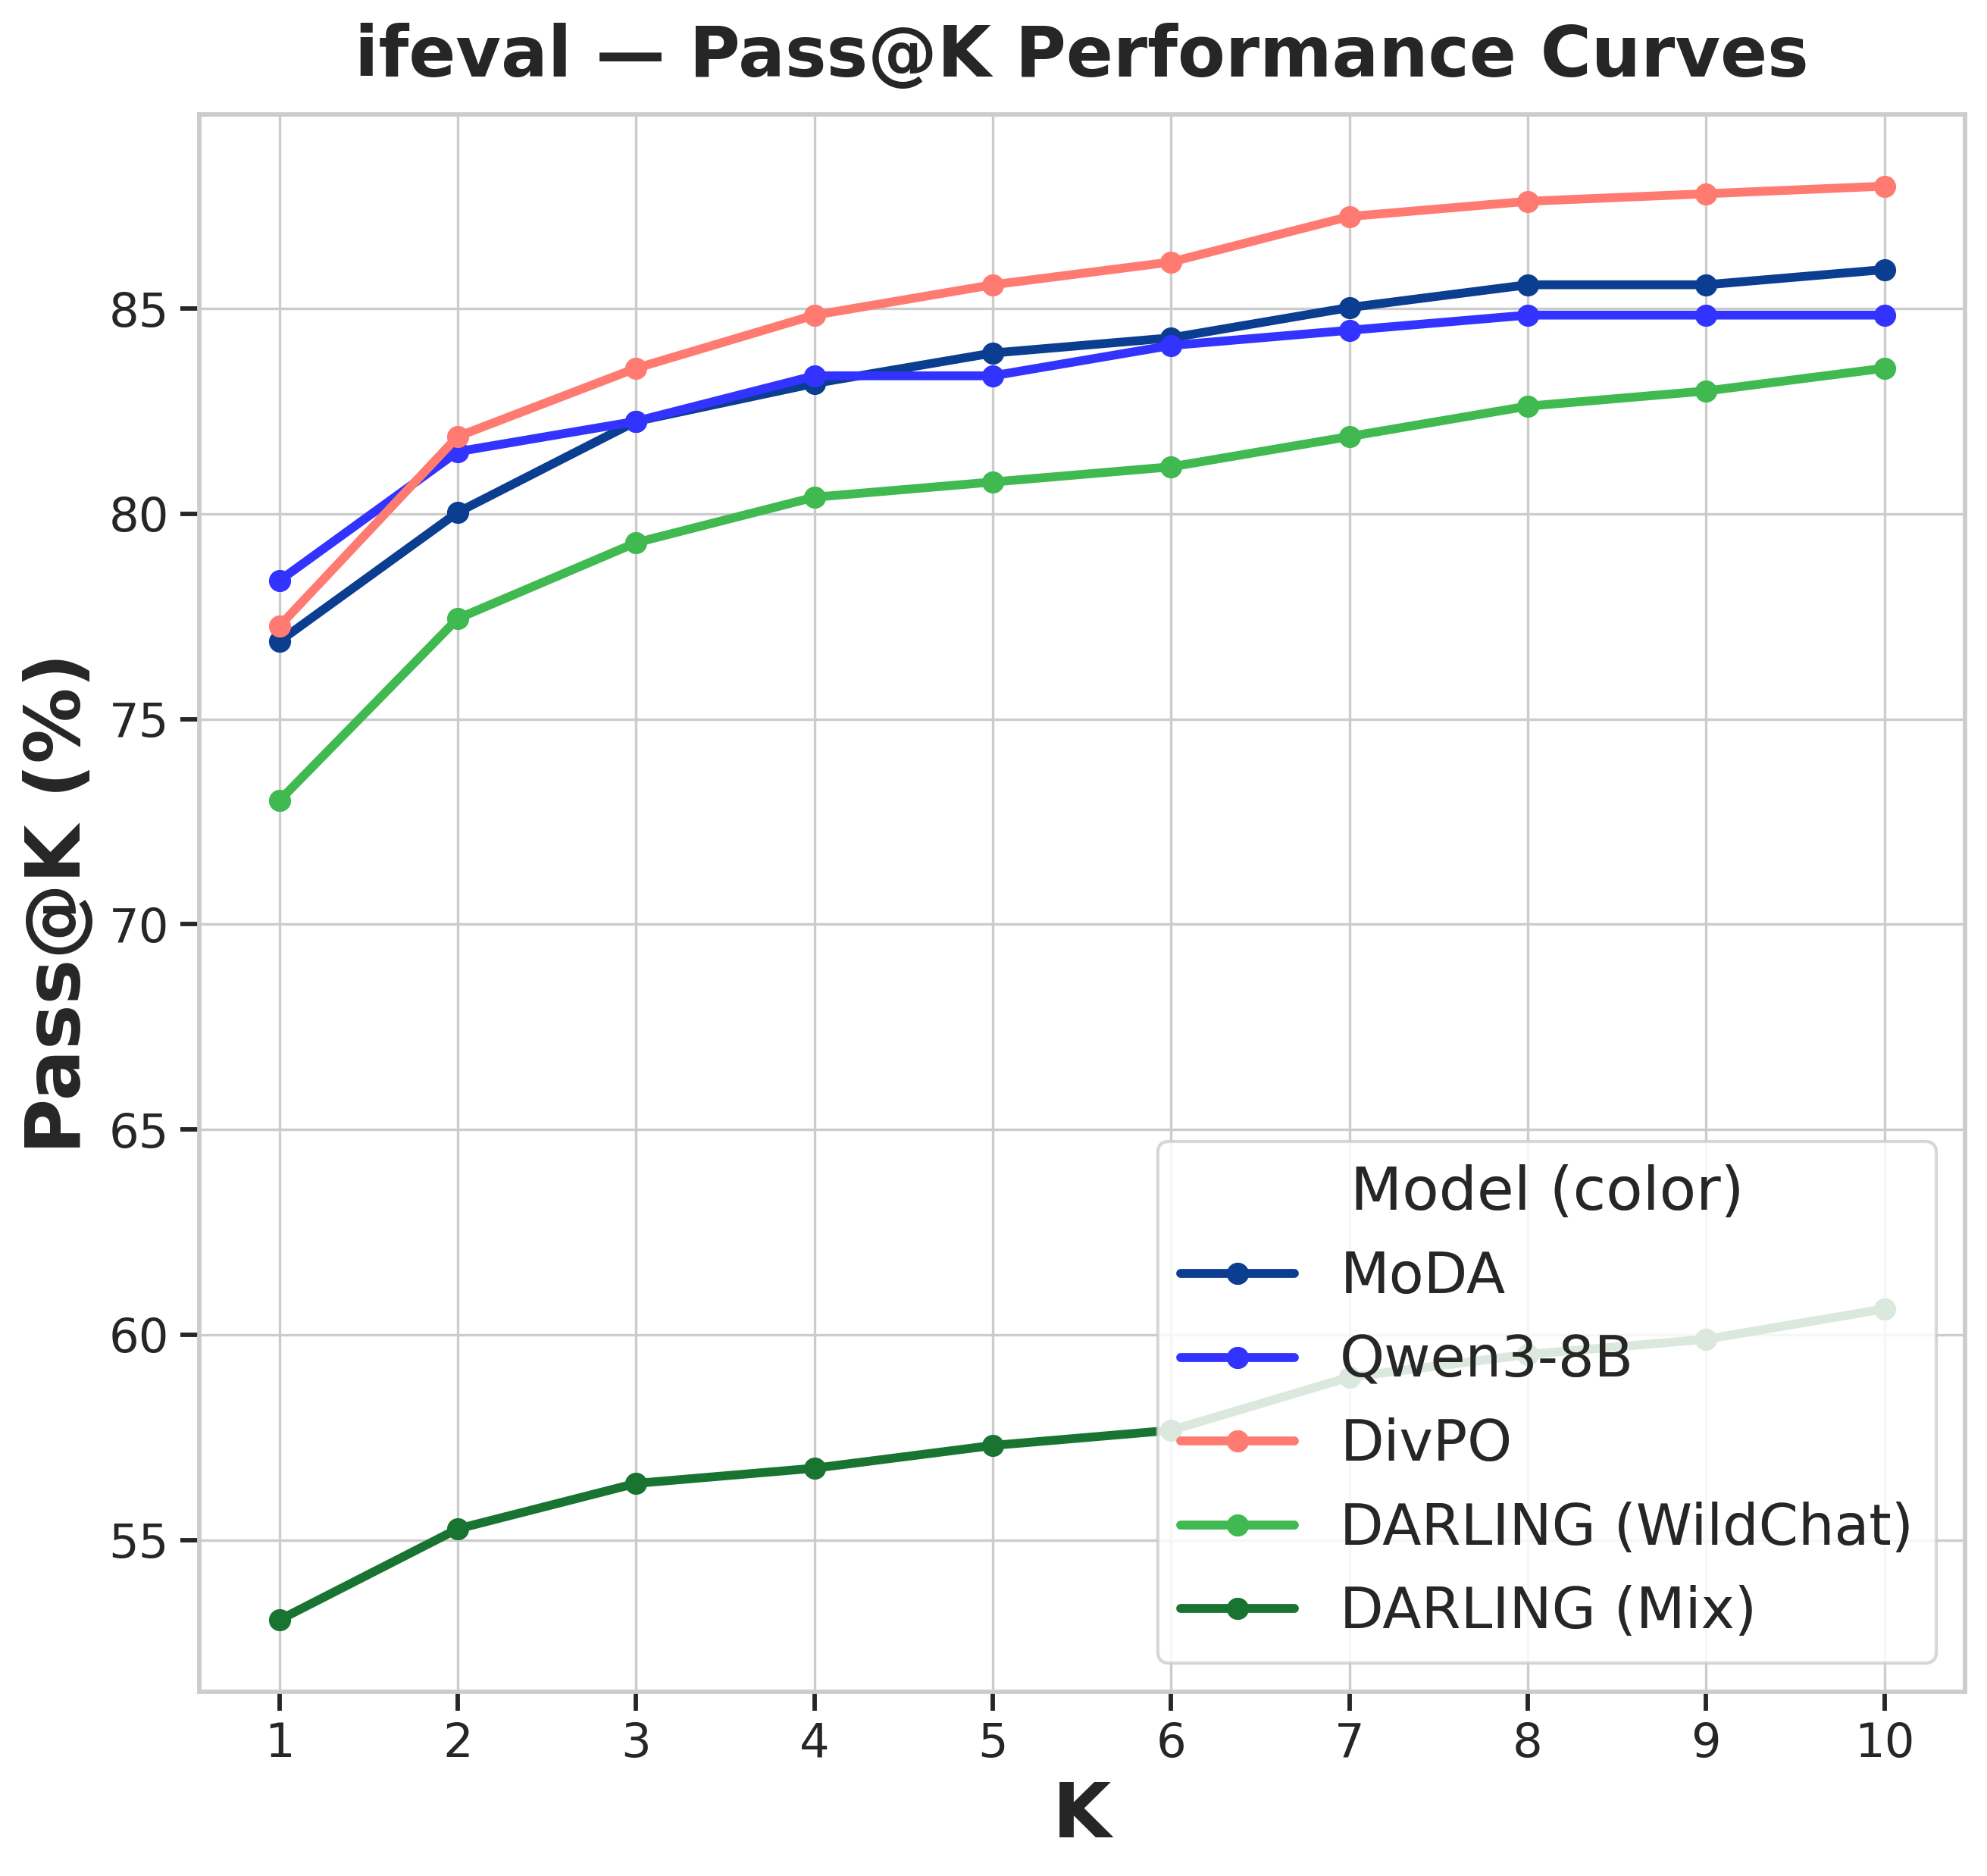
\includegraphics[width=\linewidth]{figures/main_pass_k/pass_at_k_figures/pass_at_k_ifeval_thinking_false_base_model_qwen3-8b.png}
\end{minipage}
\caption{\textbf{General capability retention: pass@k accuracy.} Qwen3-8B base and thinking disabled models on the general capability suite tasks: GSM8K, MMLU, GPQA, BoolQ, HellaSwag, TruthfulQA, and IFEval. The suite average is shown in Figure~\ref{fig:general capability pass@k} in the main text.}
\label{fig:general capability pass@k thinking disabled}
\end{figure}


\begin{figure}[H]
\begin{minipage}{0.24\textwidth}
  \centering
  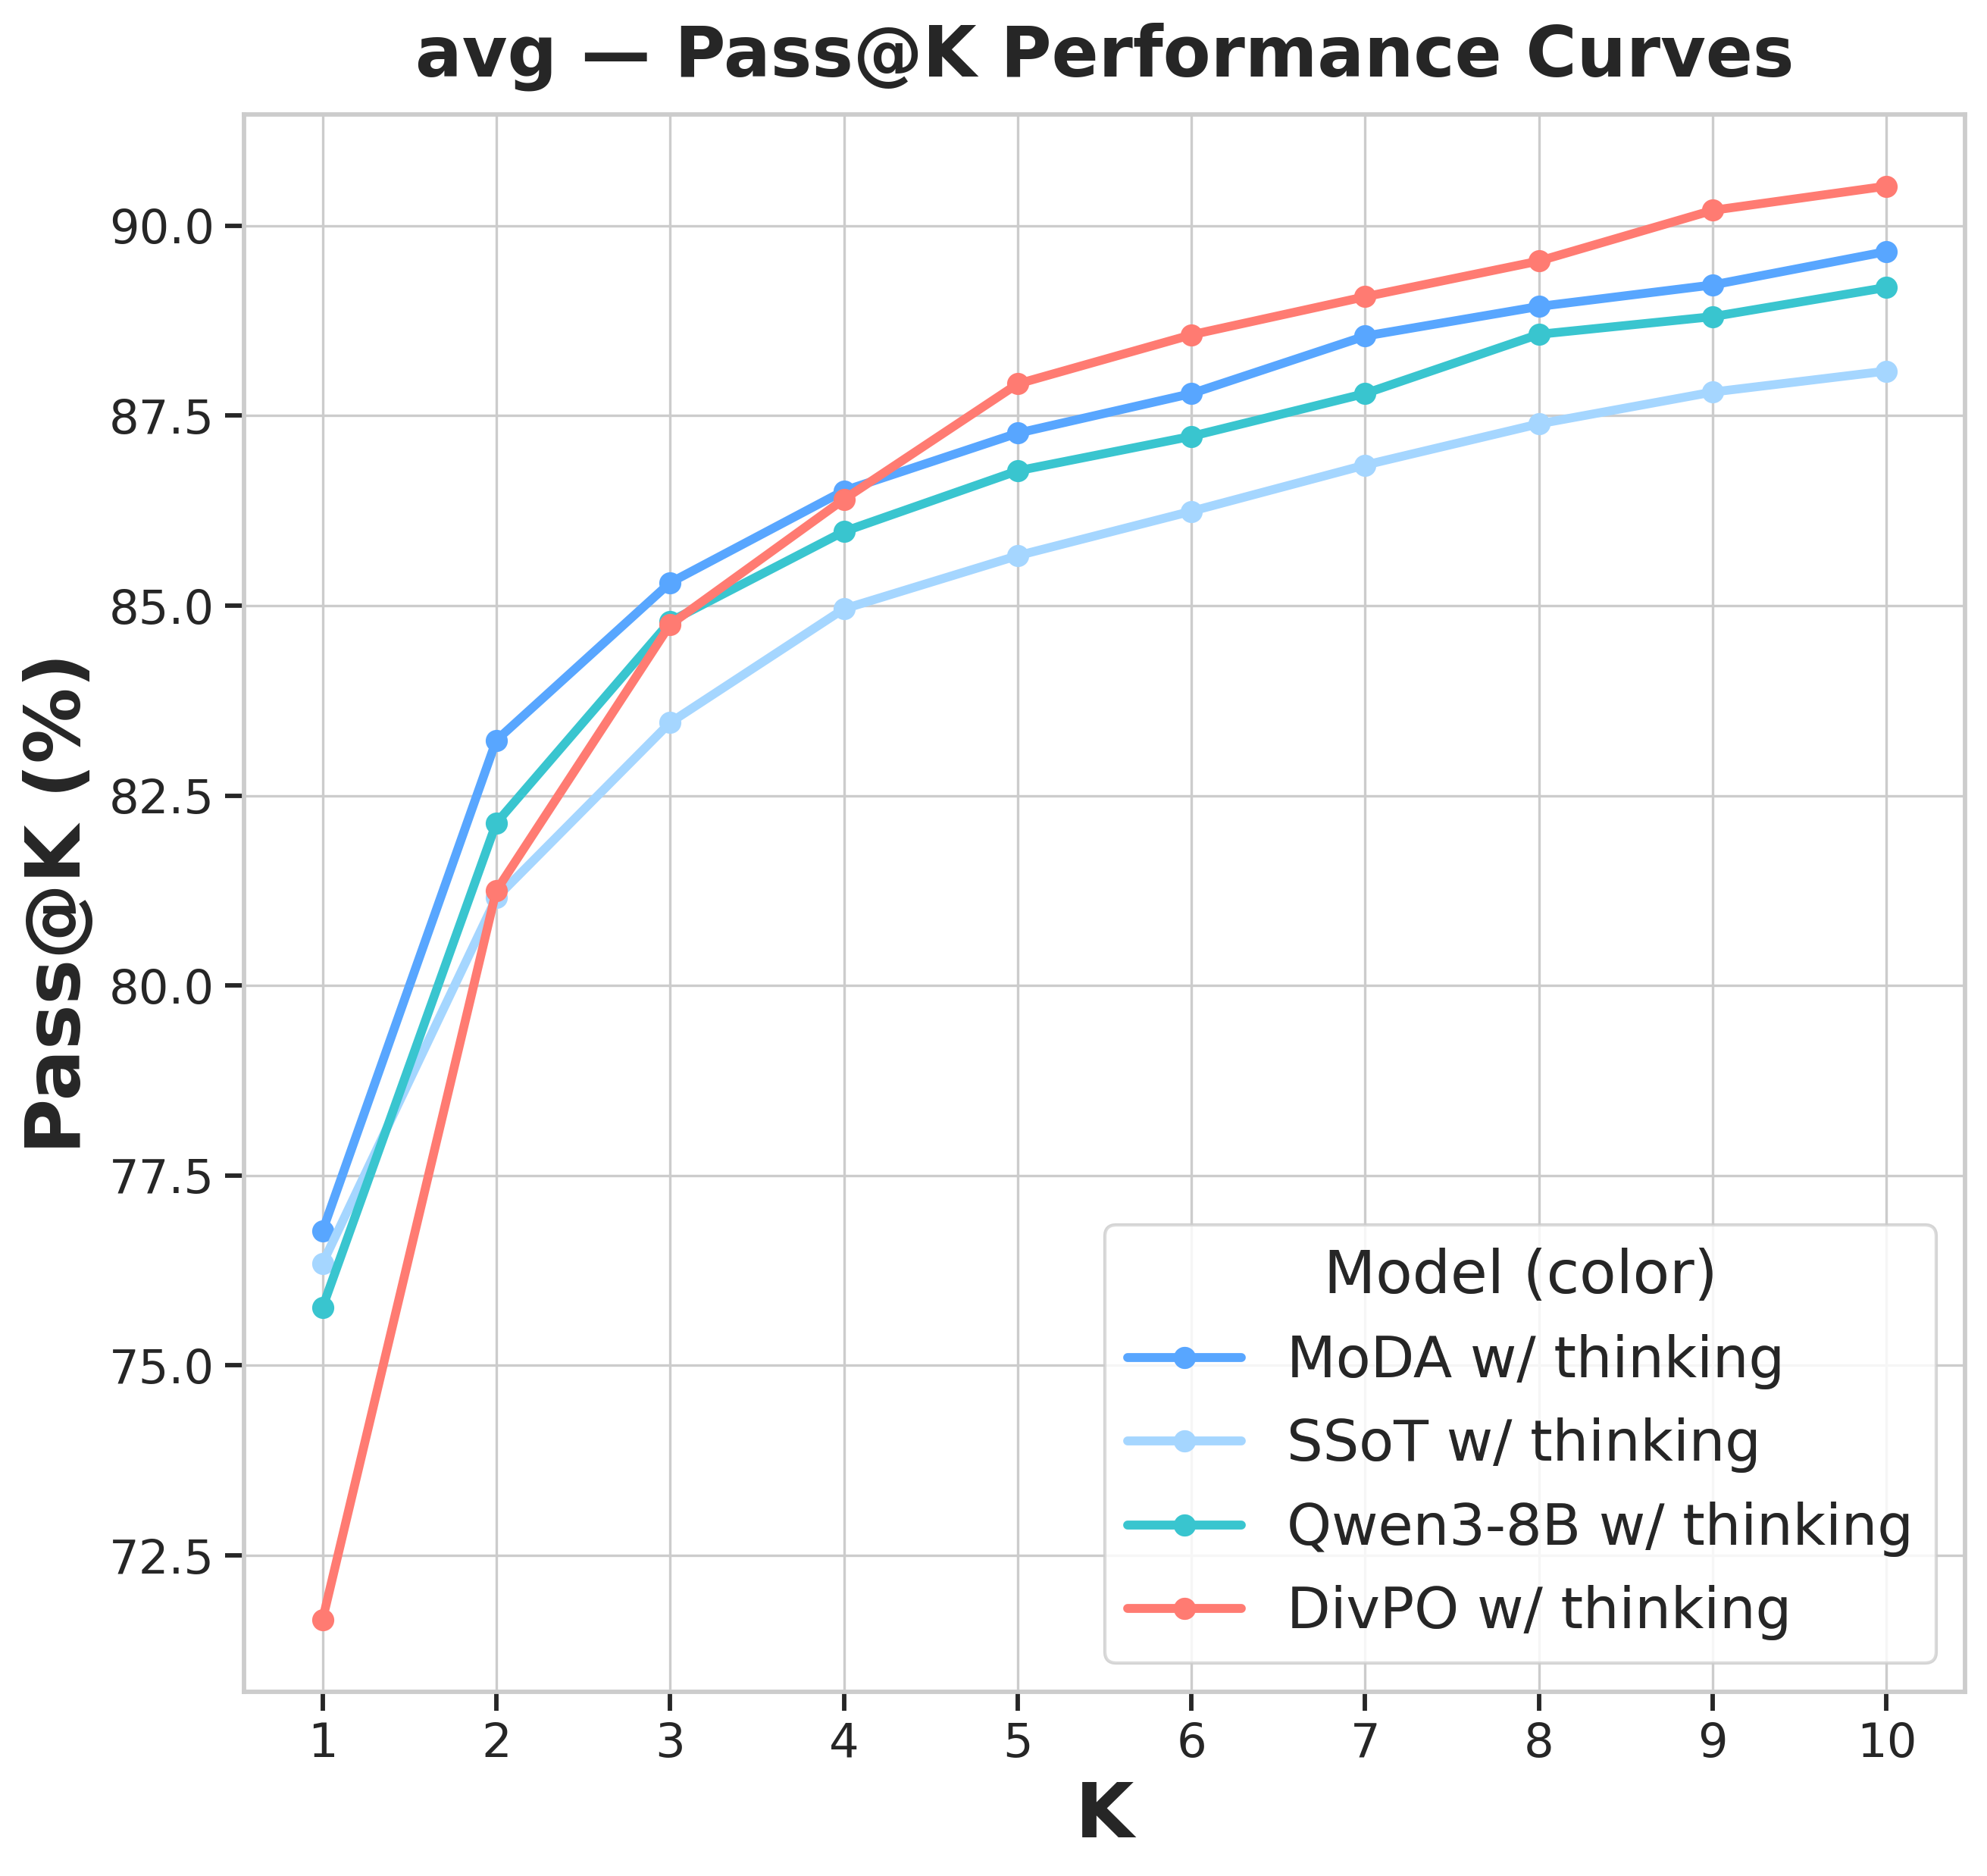
\includegraphics[width=\linewidth]{figures/main_pass_k/pass_at_k_figures/pass_at_k_avg_thinking_true.png}
\end{minipage}\hfill
\centering
\begin{minipage}{0.24\textwidth}
  \centering
  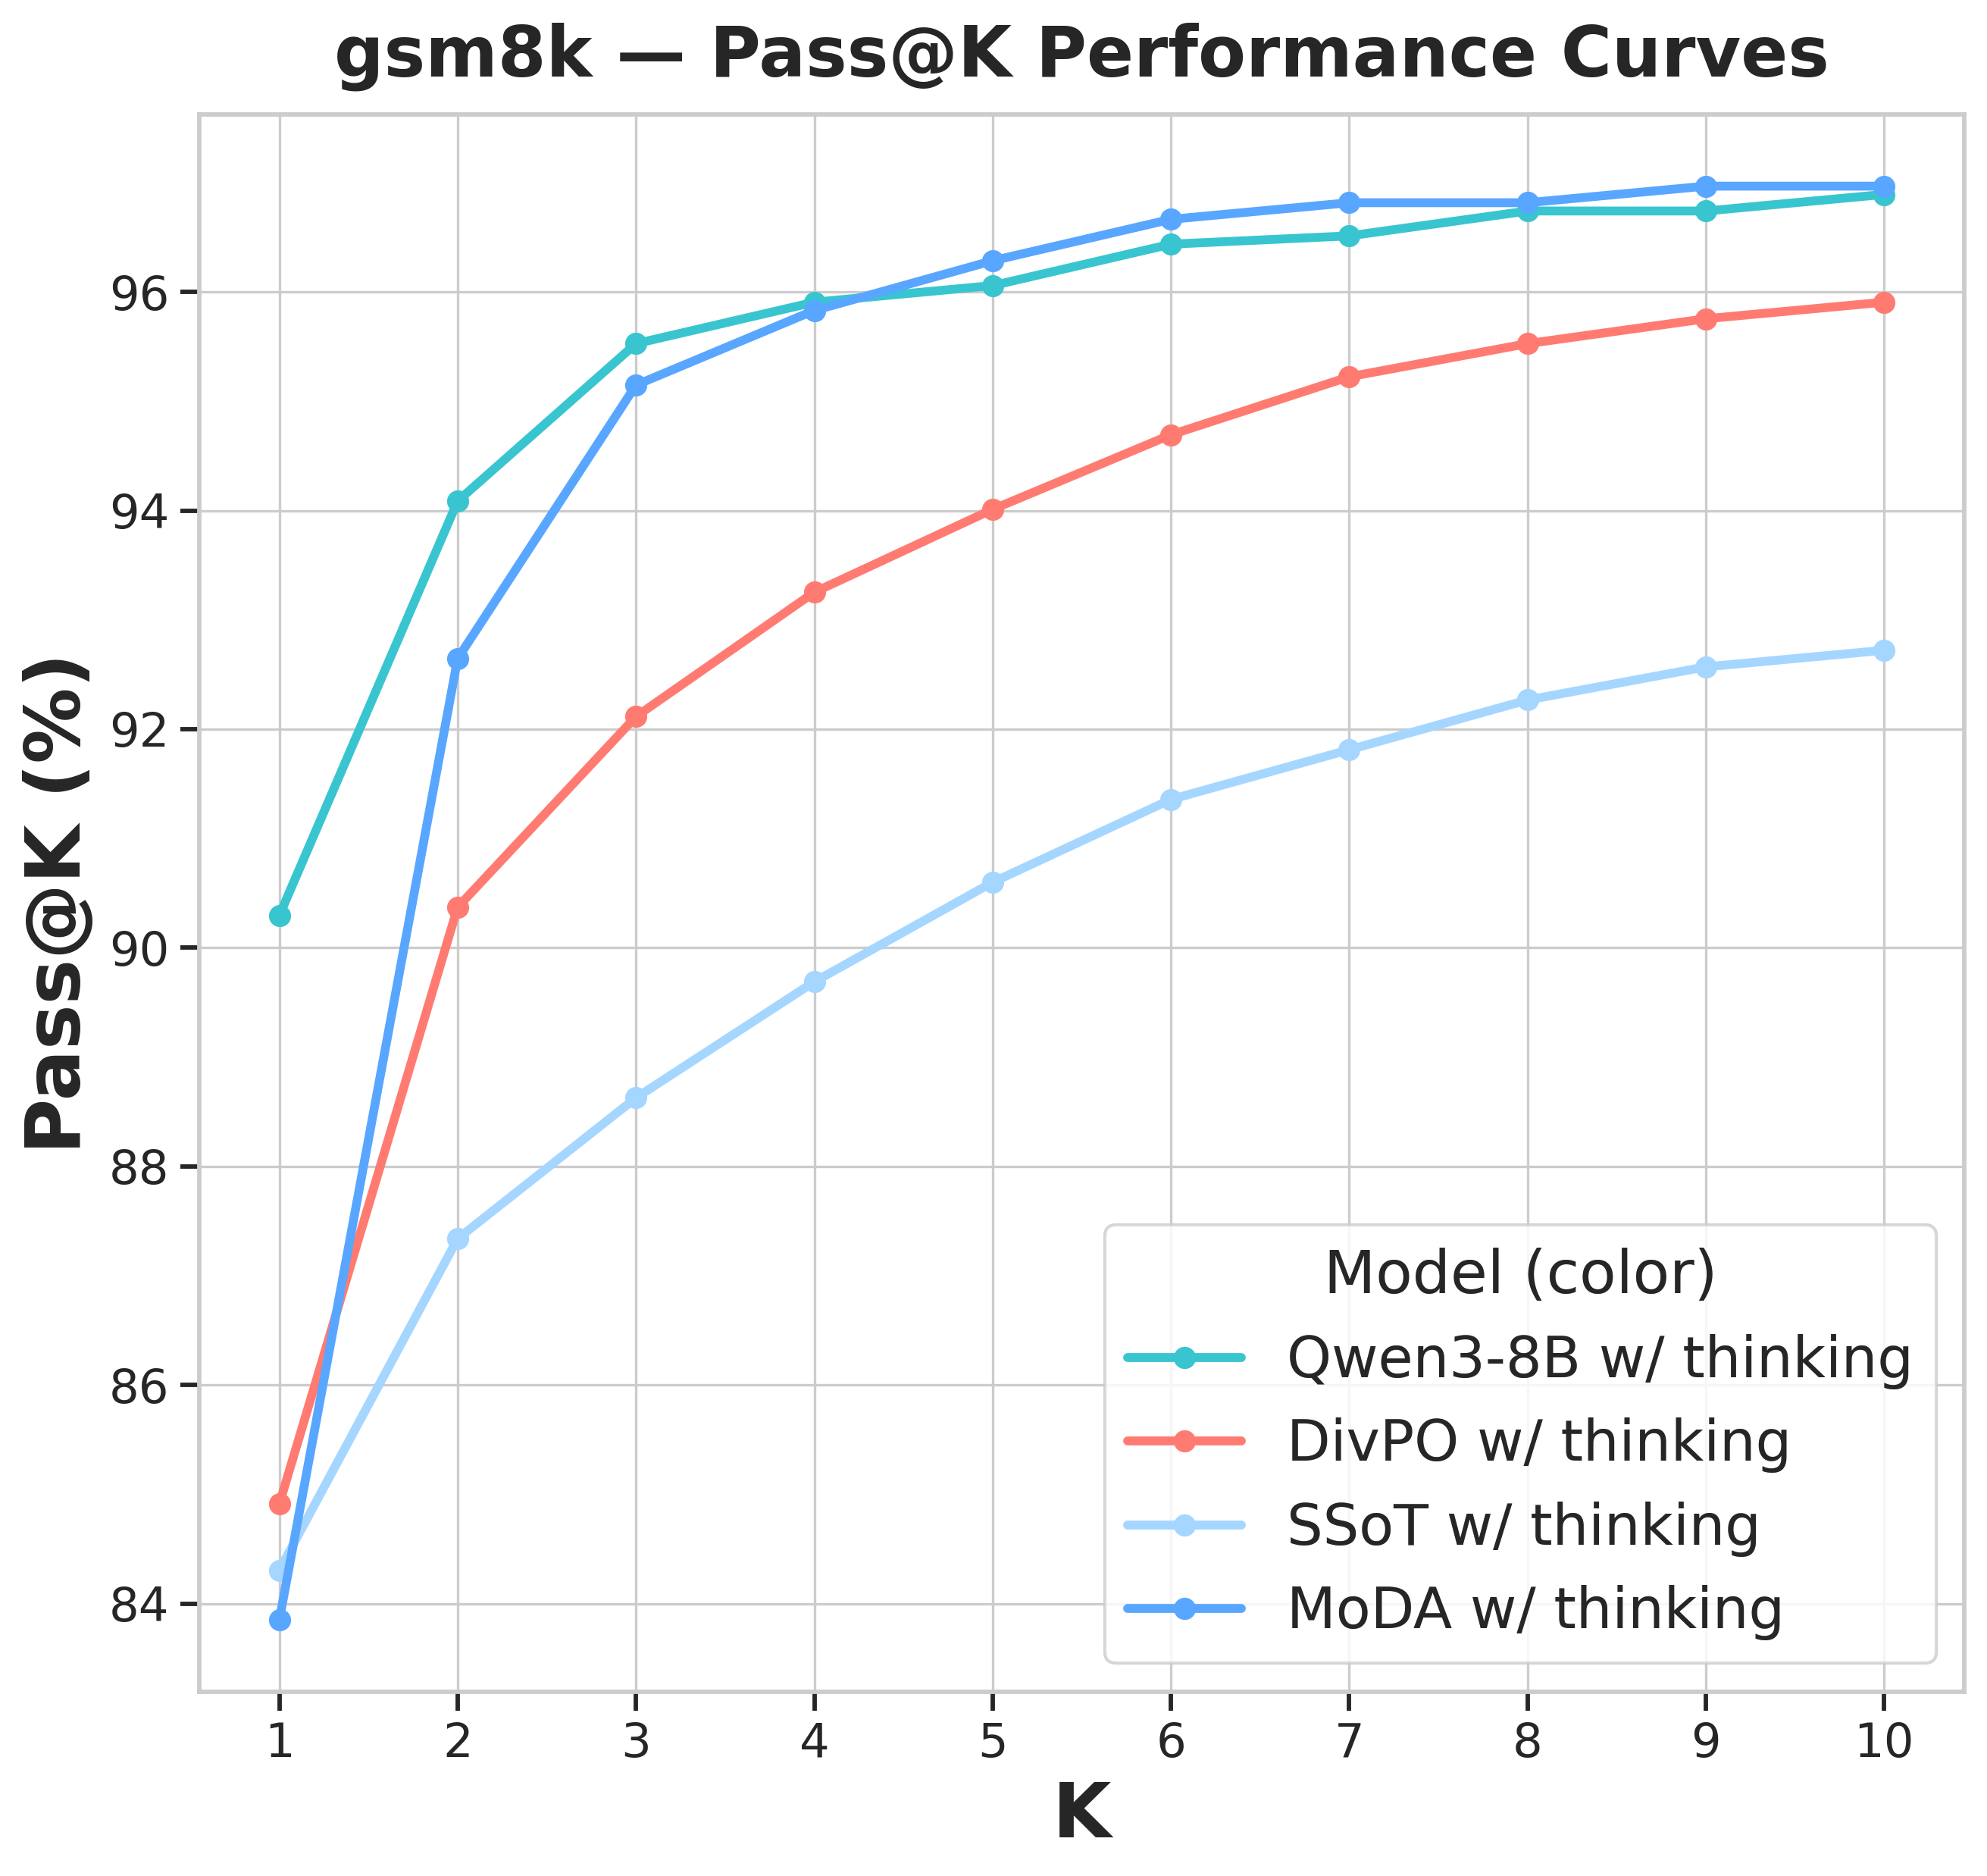
\includegraphics[width=\linewidth]{figures/main_pass_k/pass_at_k_figures/pass_at_k_gsm8k_thinking_true.png}
\end{minipage}\hfill
\begin{minipage}{0.24\textwidth}
  \centering
  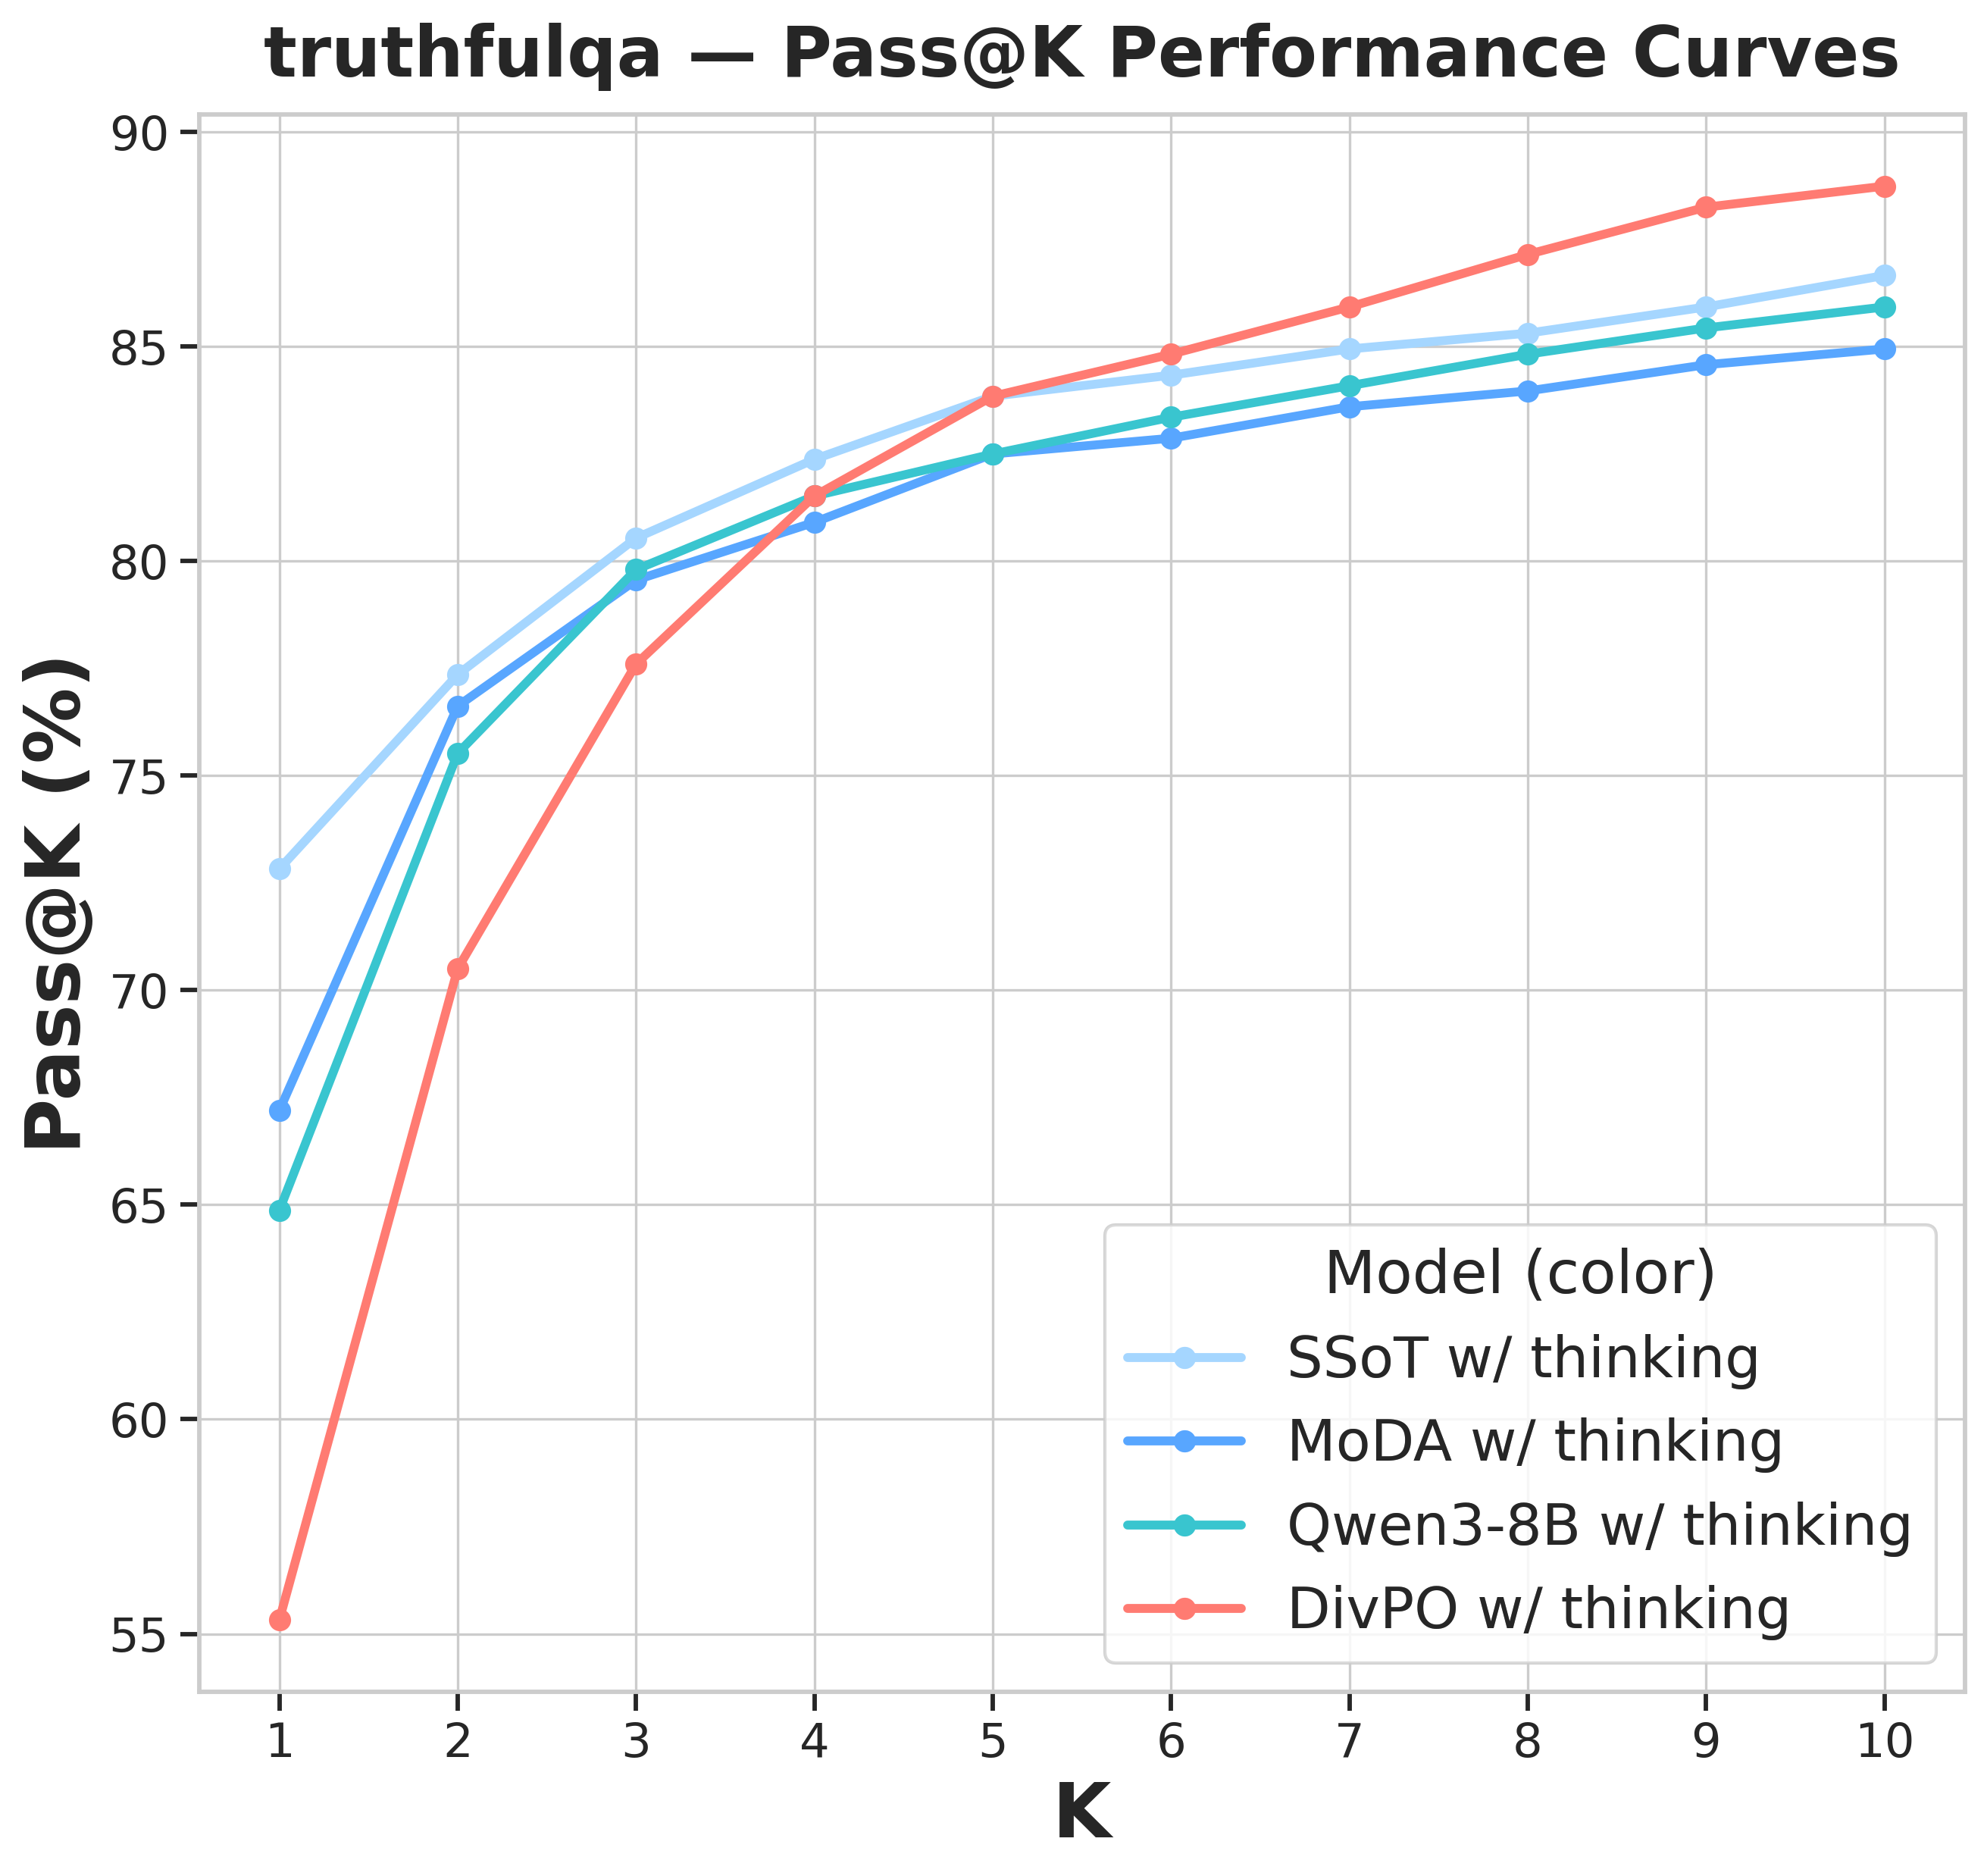
\includegraphics[width=\linewidth]{figures/main_pass_k/pass_at_k_figures/pass_at_k_truthfulqa_thinking_true.png}
\end{minipage}\hfill
\begin{minipage}{0.24\textwidth}
  \centering
  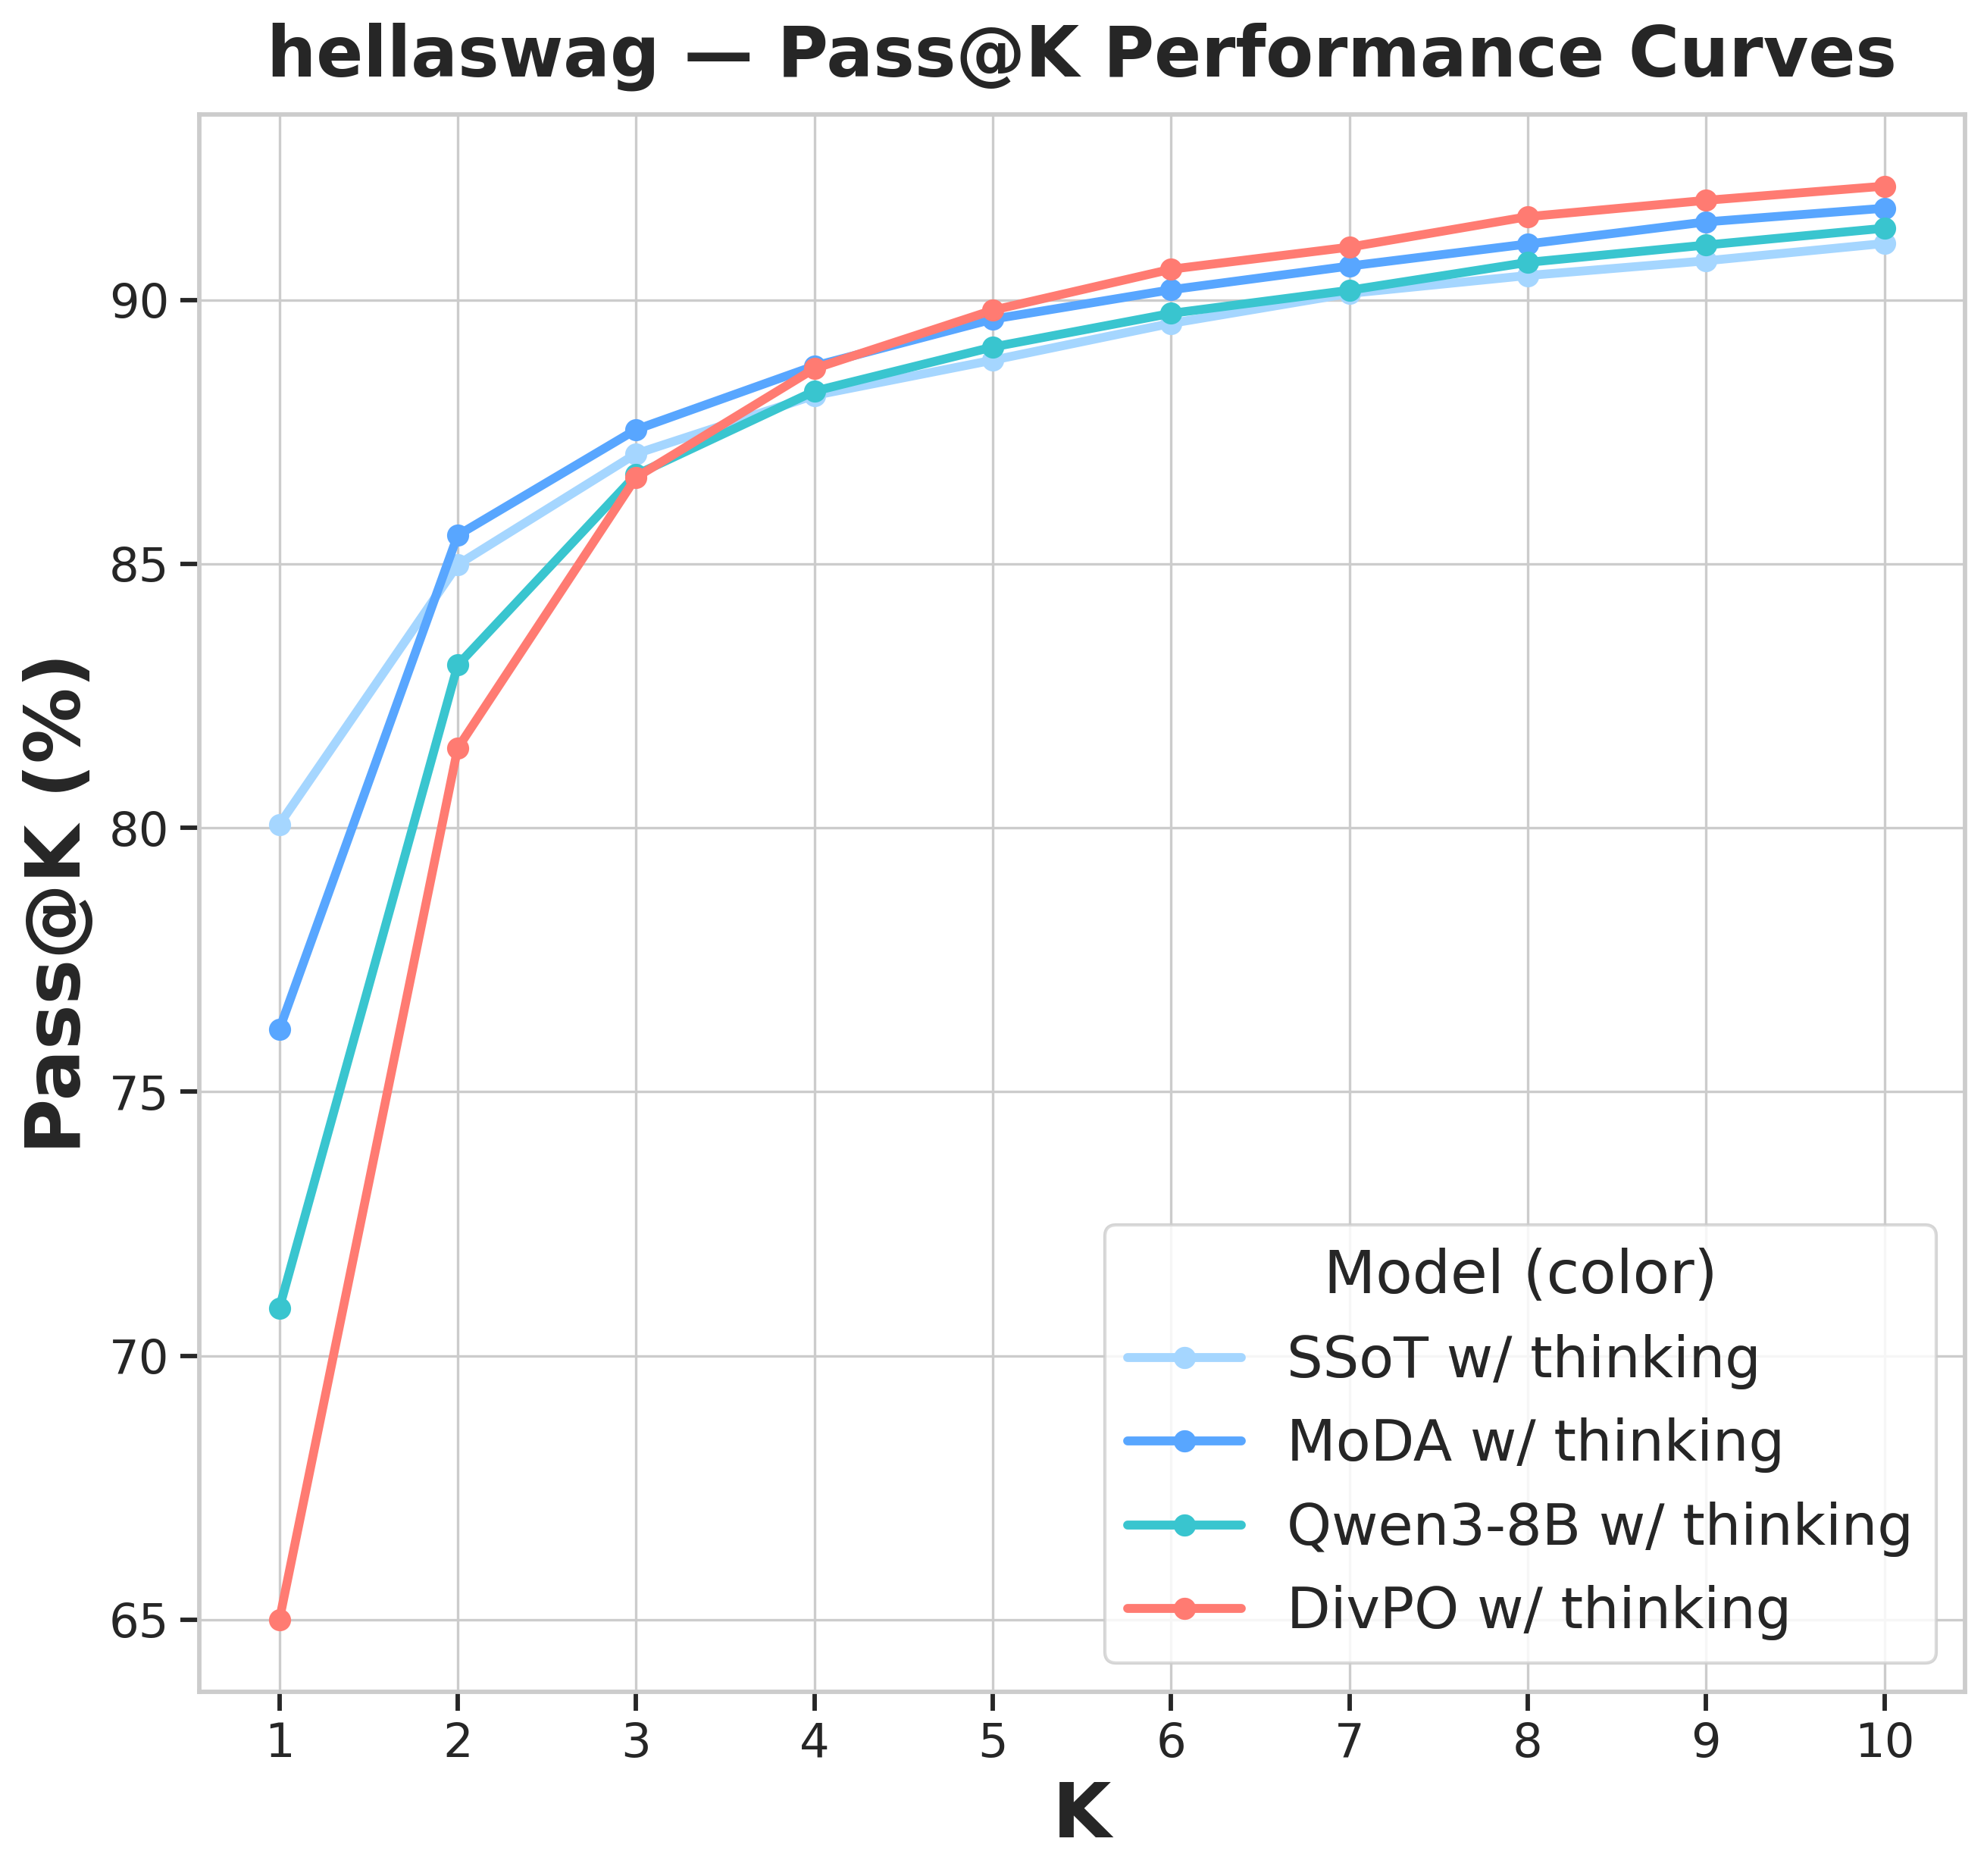
\includegraphics[width=\linewidth]{figures/main_pass_k/pass_at_k_figures/pass_at_k_hellaswag_thinking_true.png}
\end{minipage}
\centering
\begin{minipage}{0.24\textwidth}
  \centering
  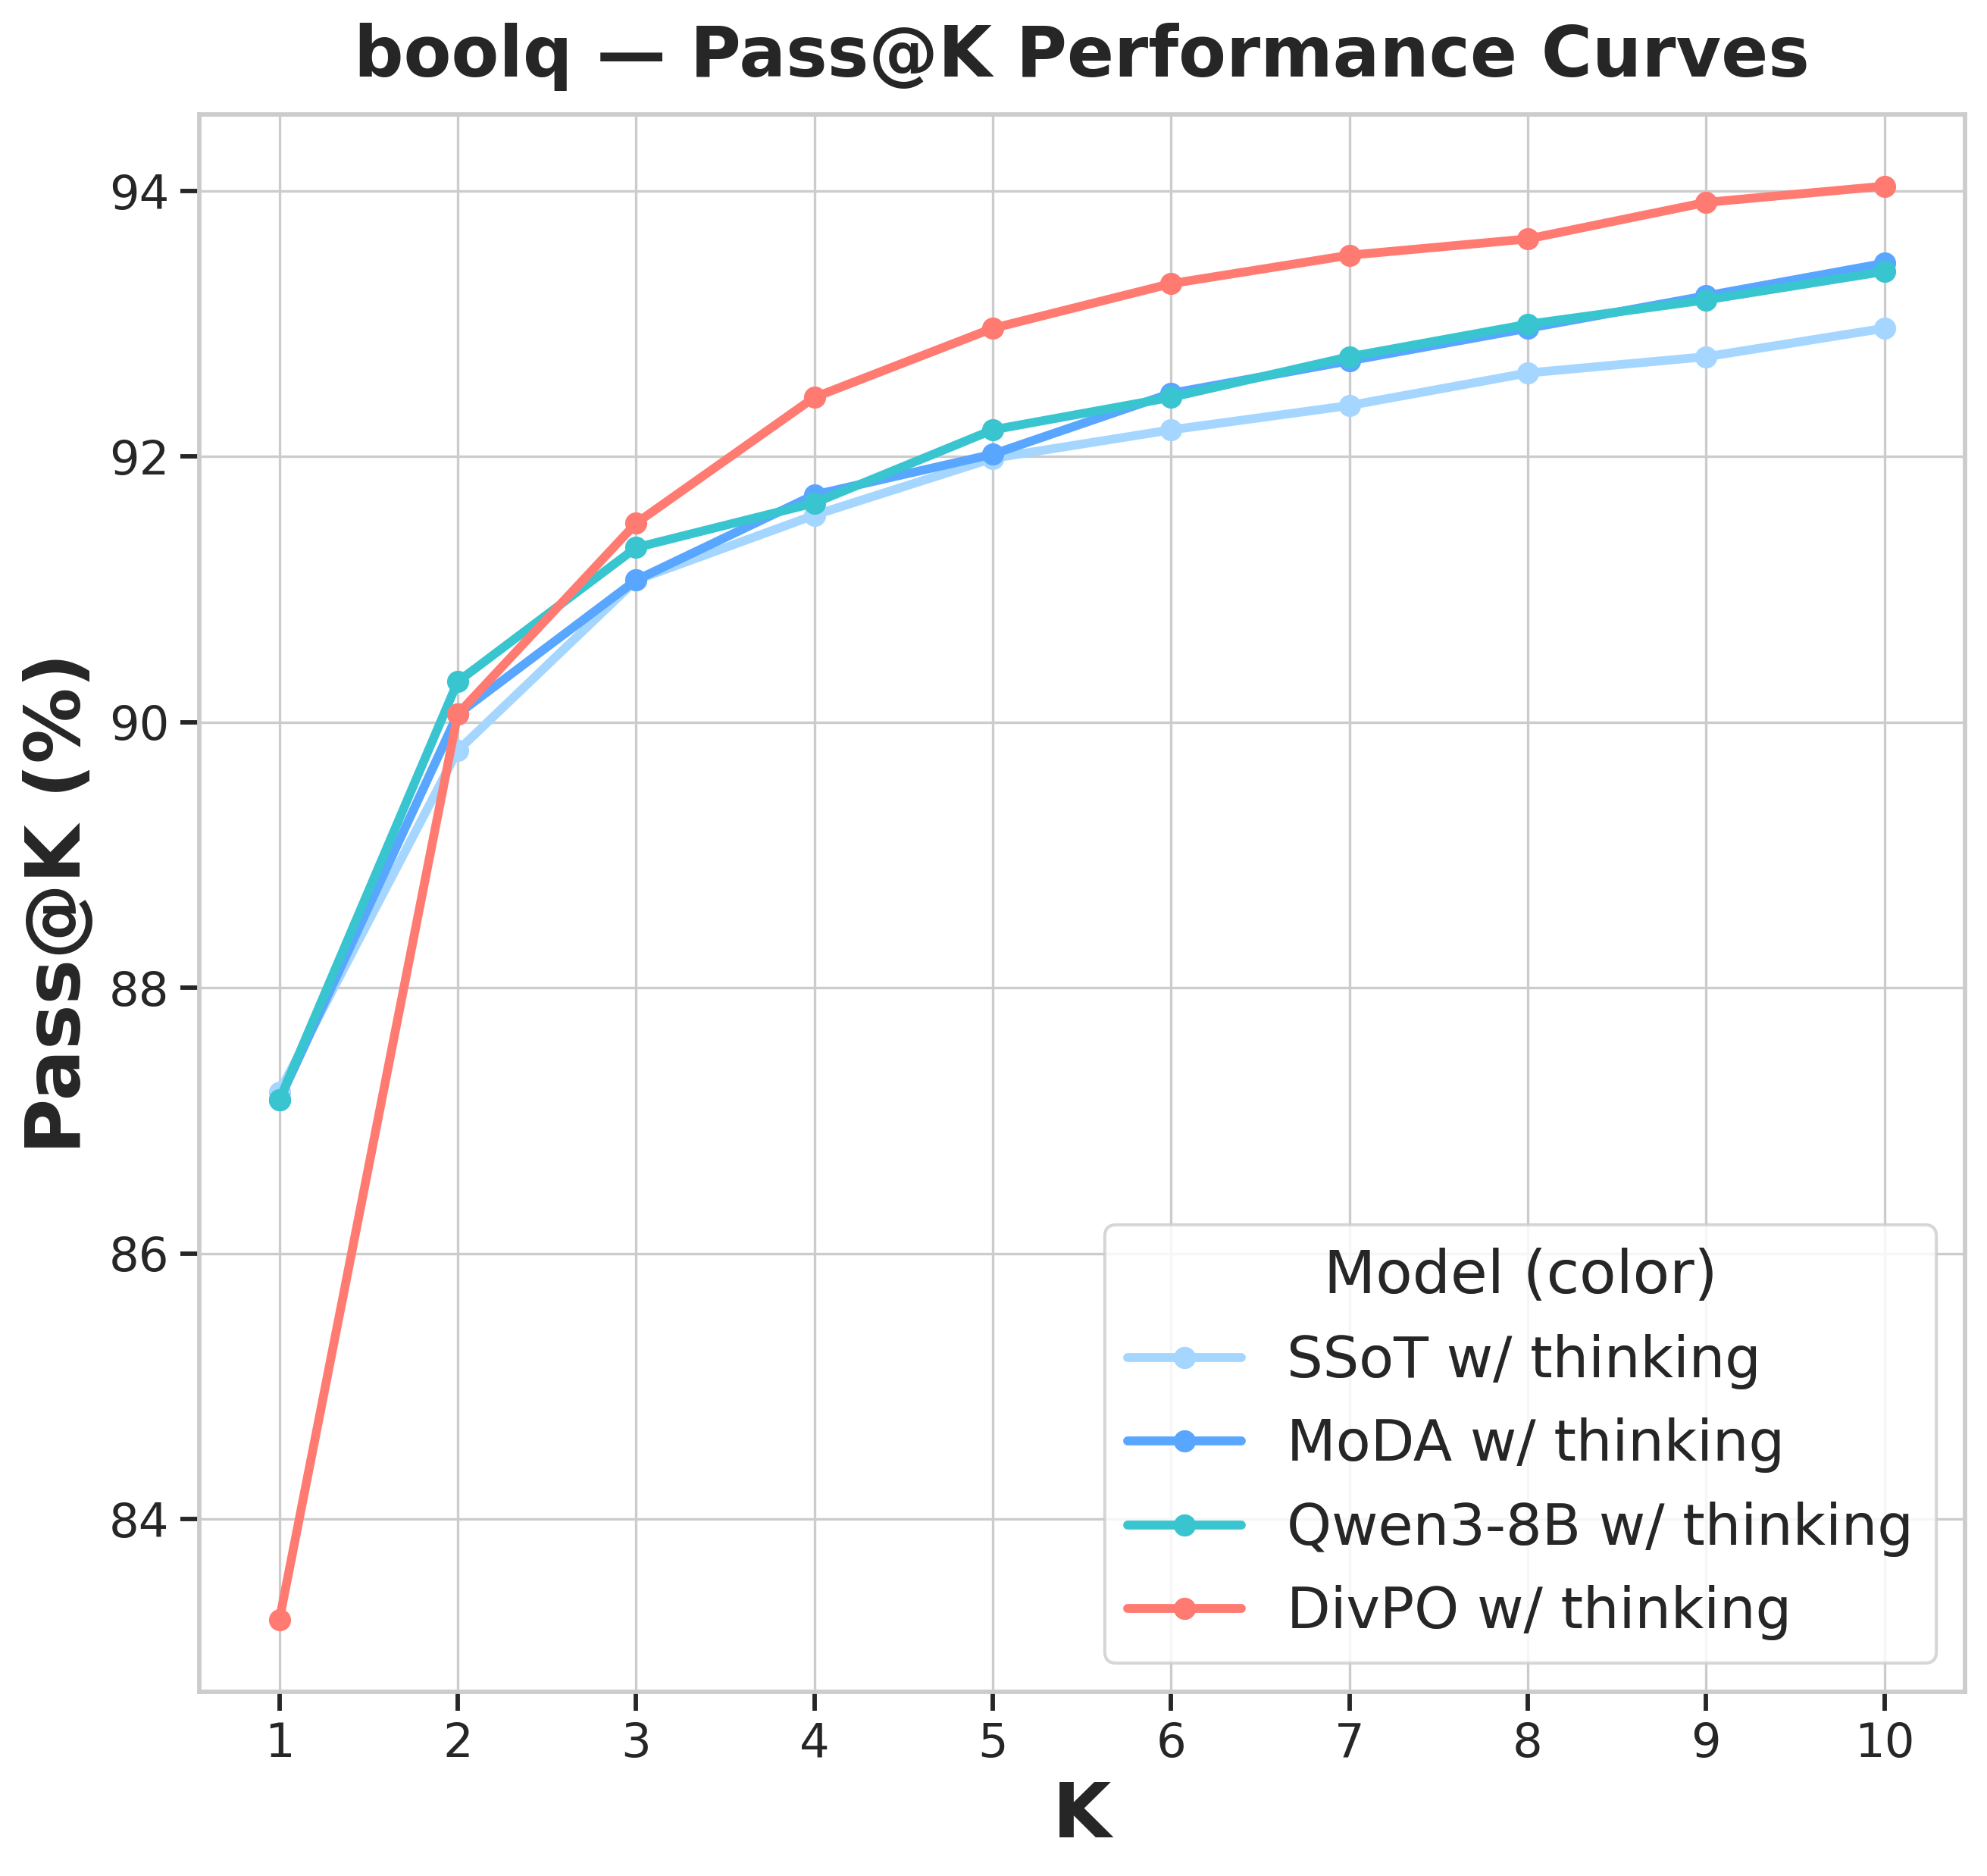
\includegraphics[width=\linewidth]{figures/main_pass_k/pass_at_k_figures/pass_at_k_boolq_thinking_true.png}
\end{minipage}\hfill
\centering
\begin{minipage}{0.24\textwidth}
  \centering
  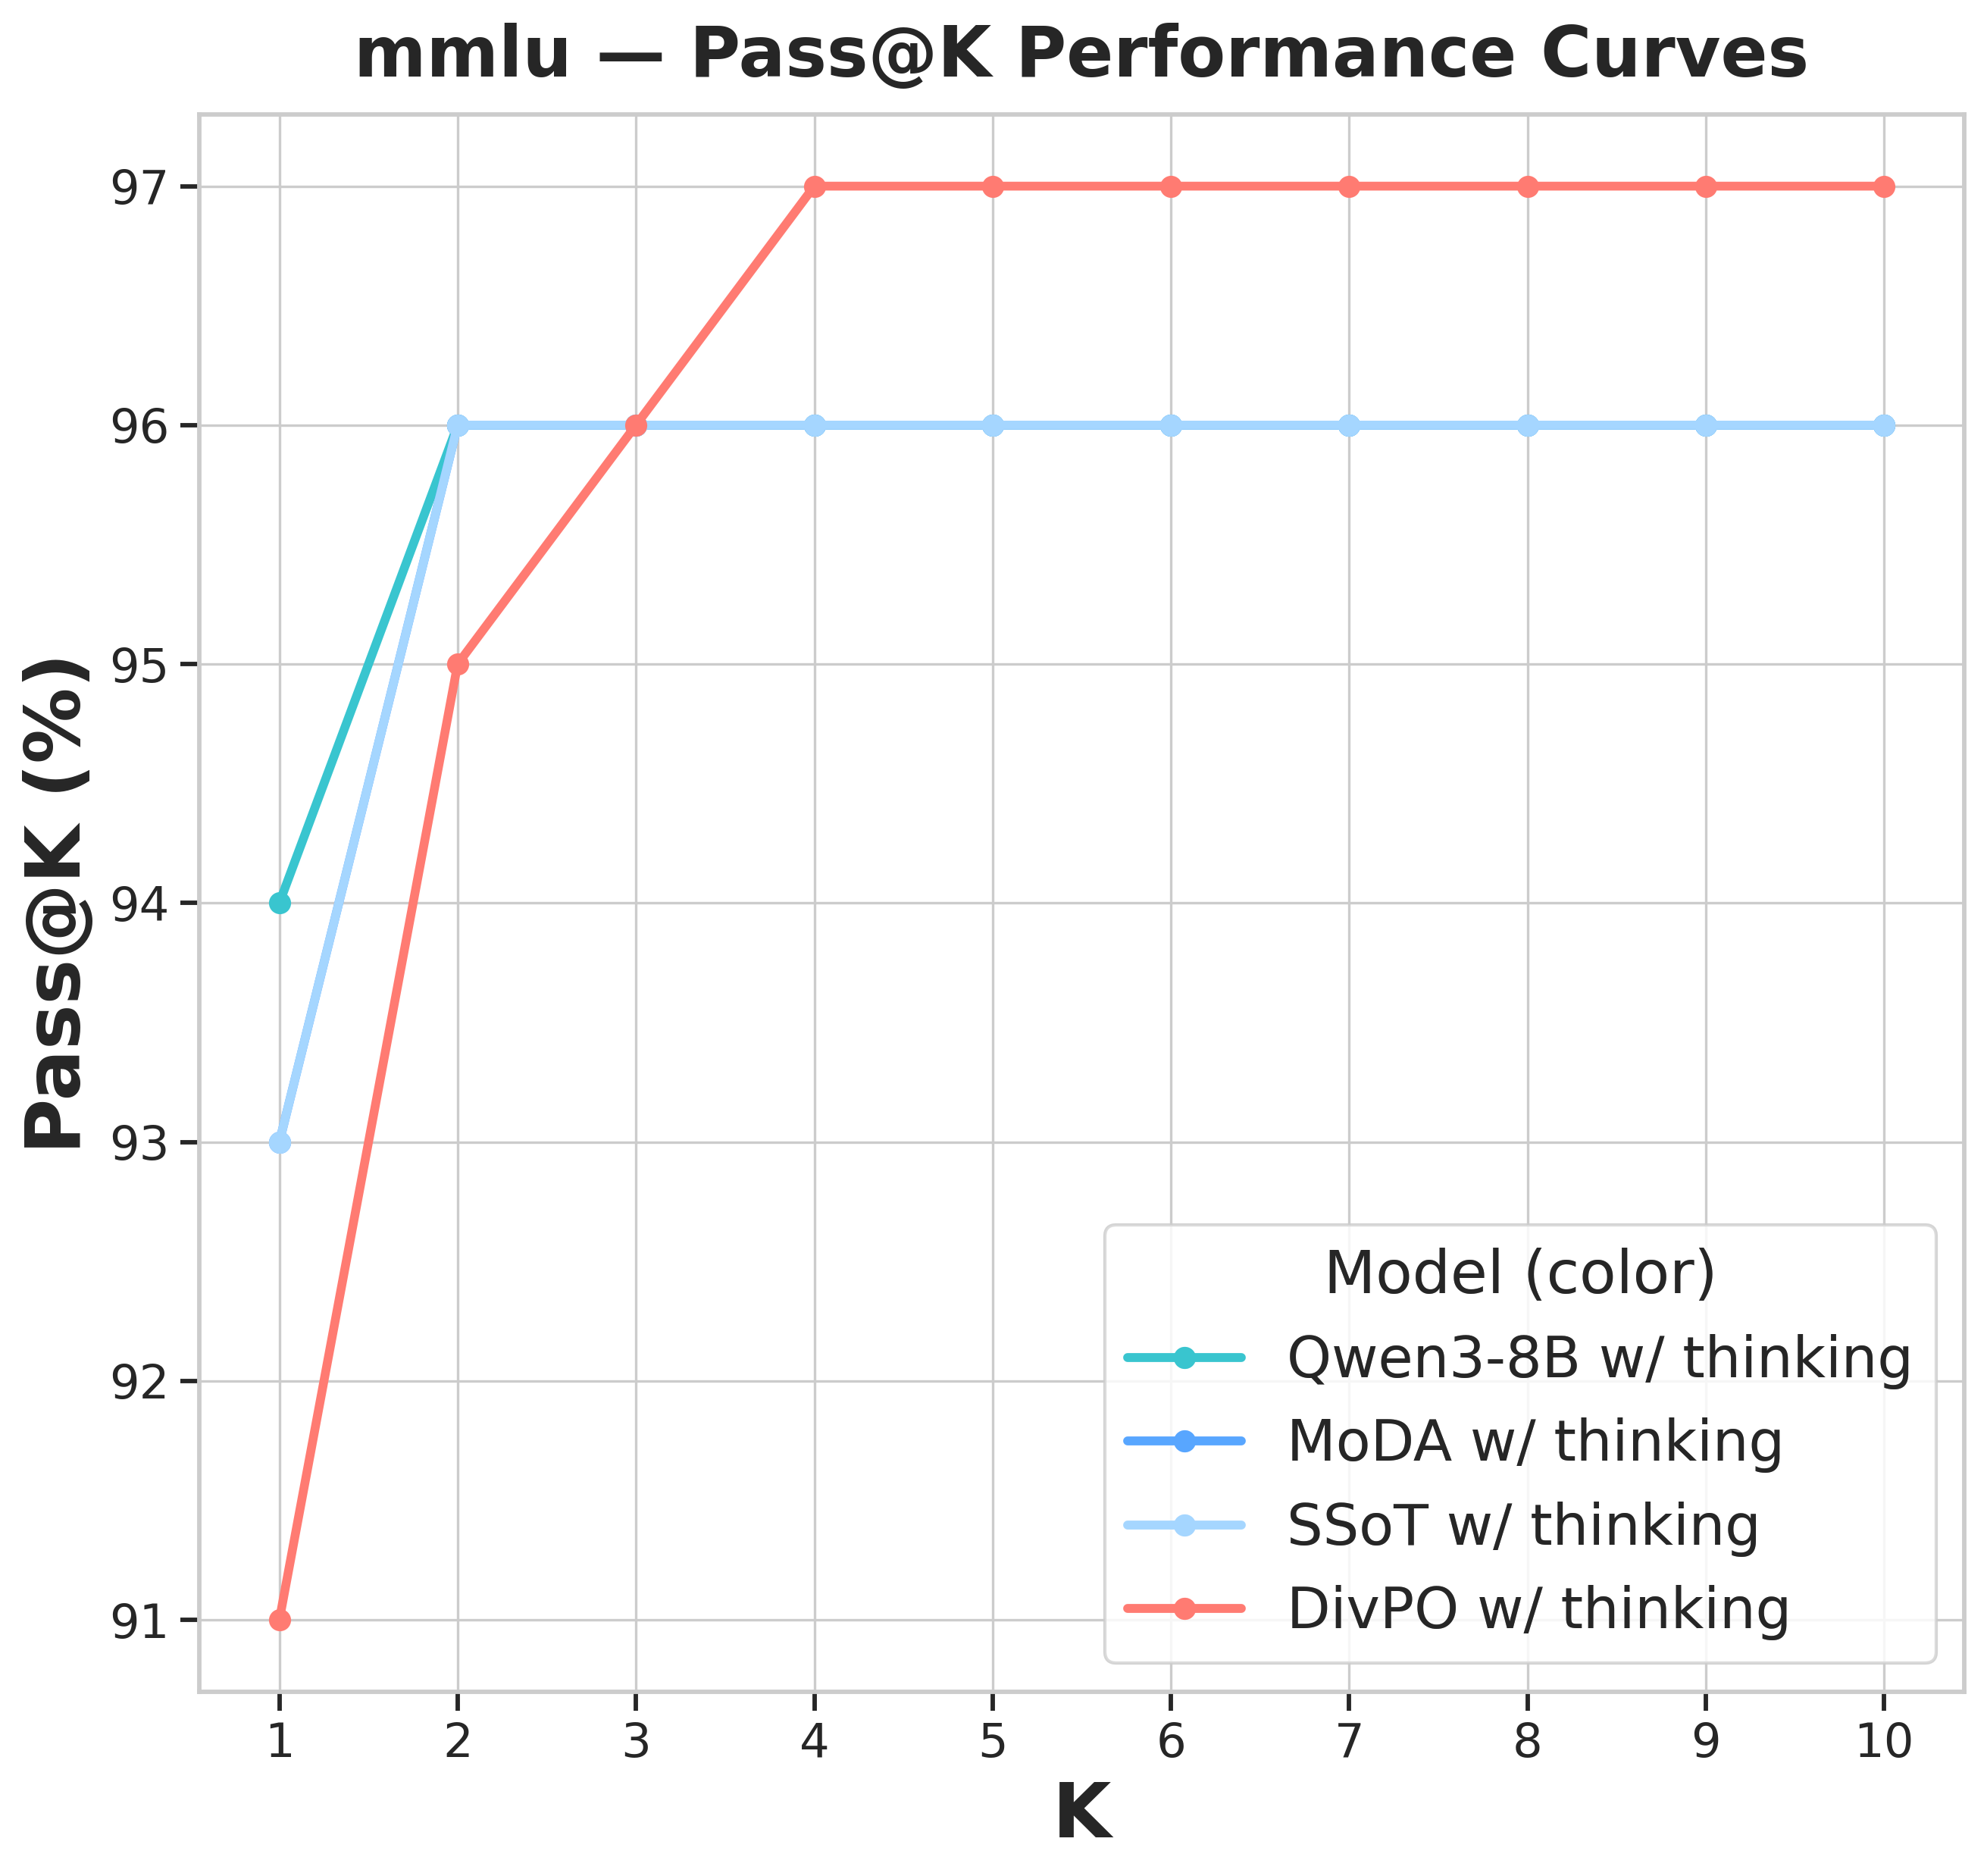
\includegraphics[width=\linewidth]{figures/main_pass_k/pass_at_k_figures/pass_at_k_mmlu_thinking_true.png}
\end{minipage}\hfill
\begin{minipage}{0.24\textwidth}
  \centering
  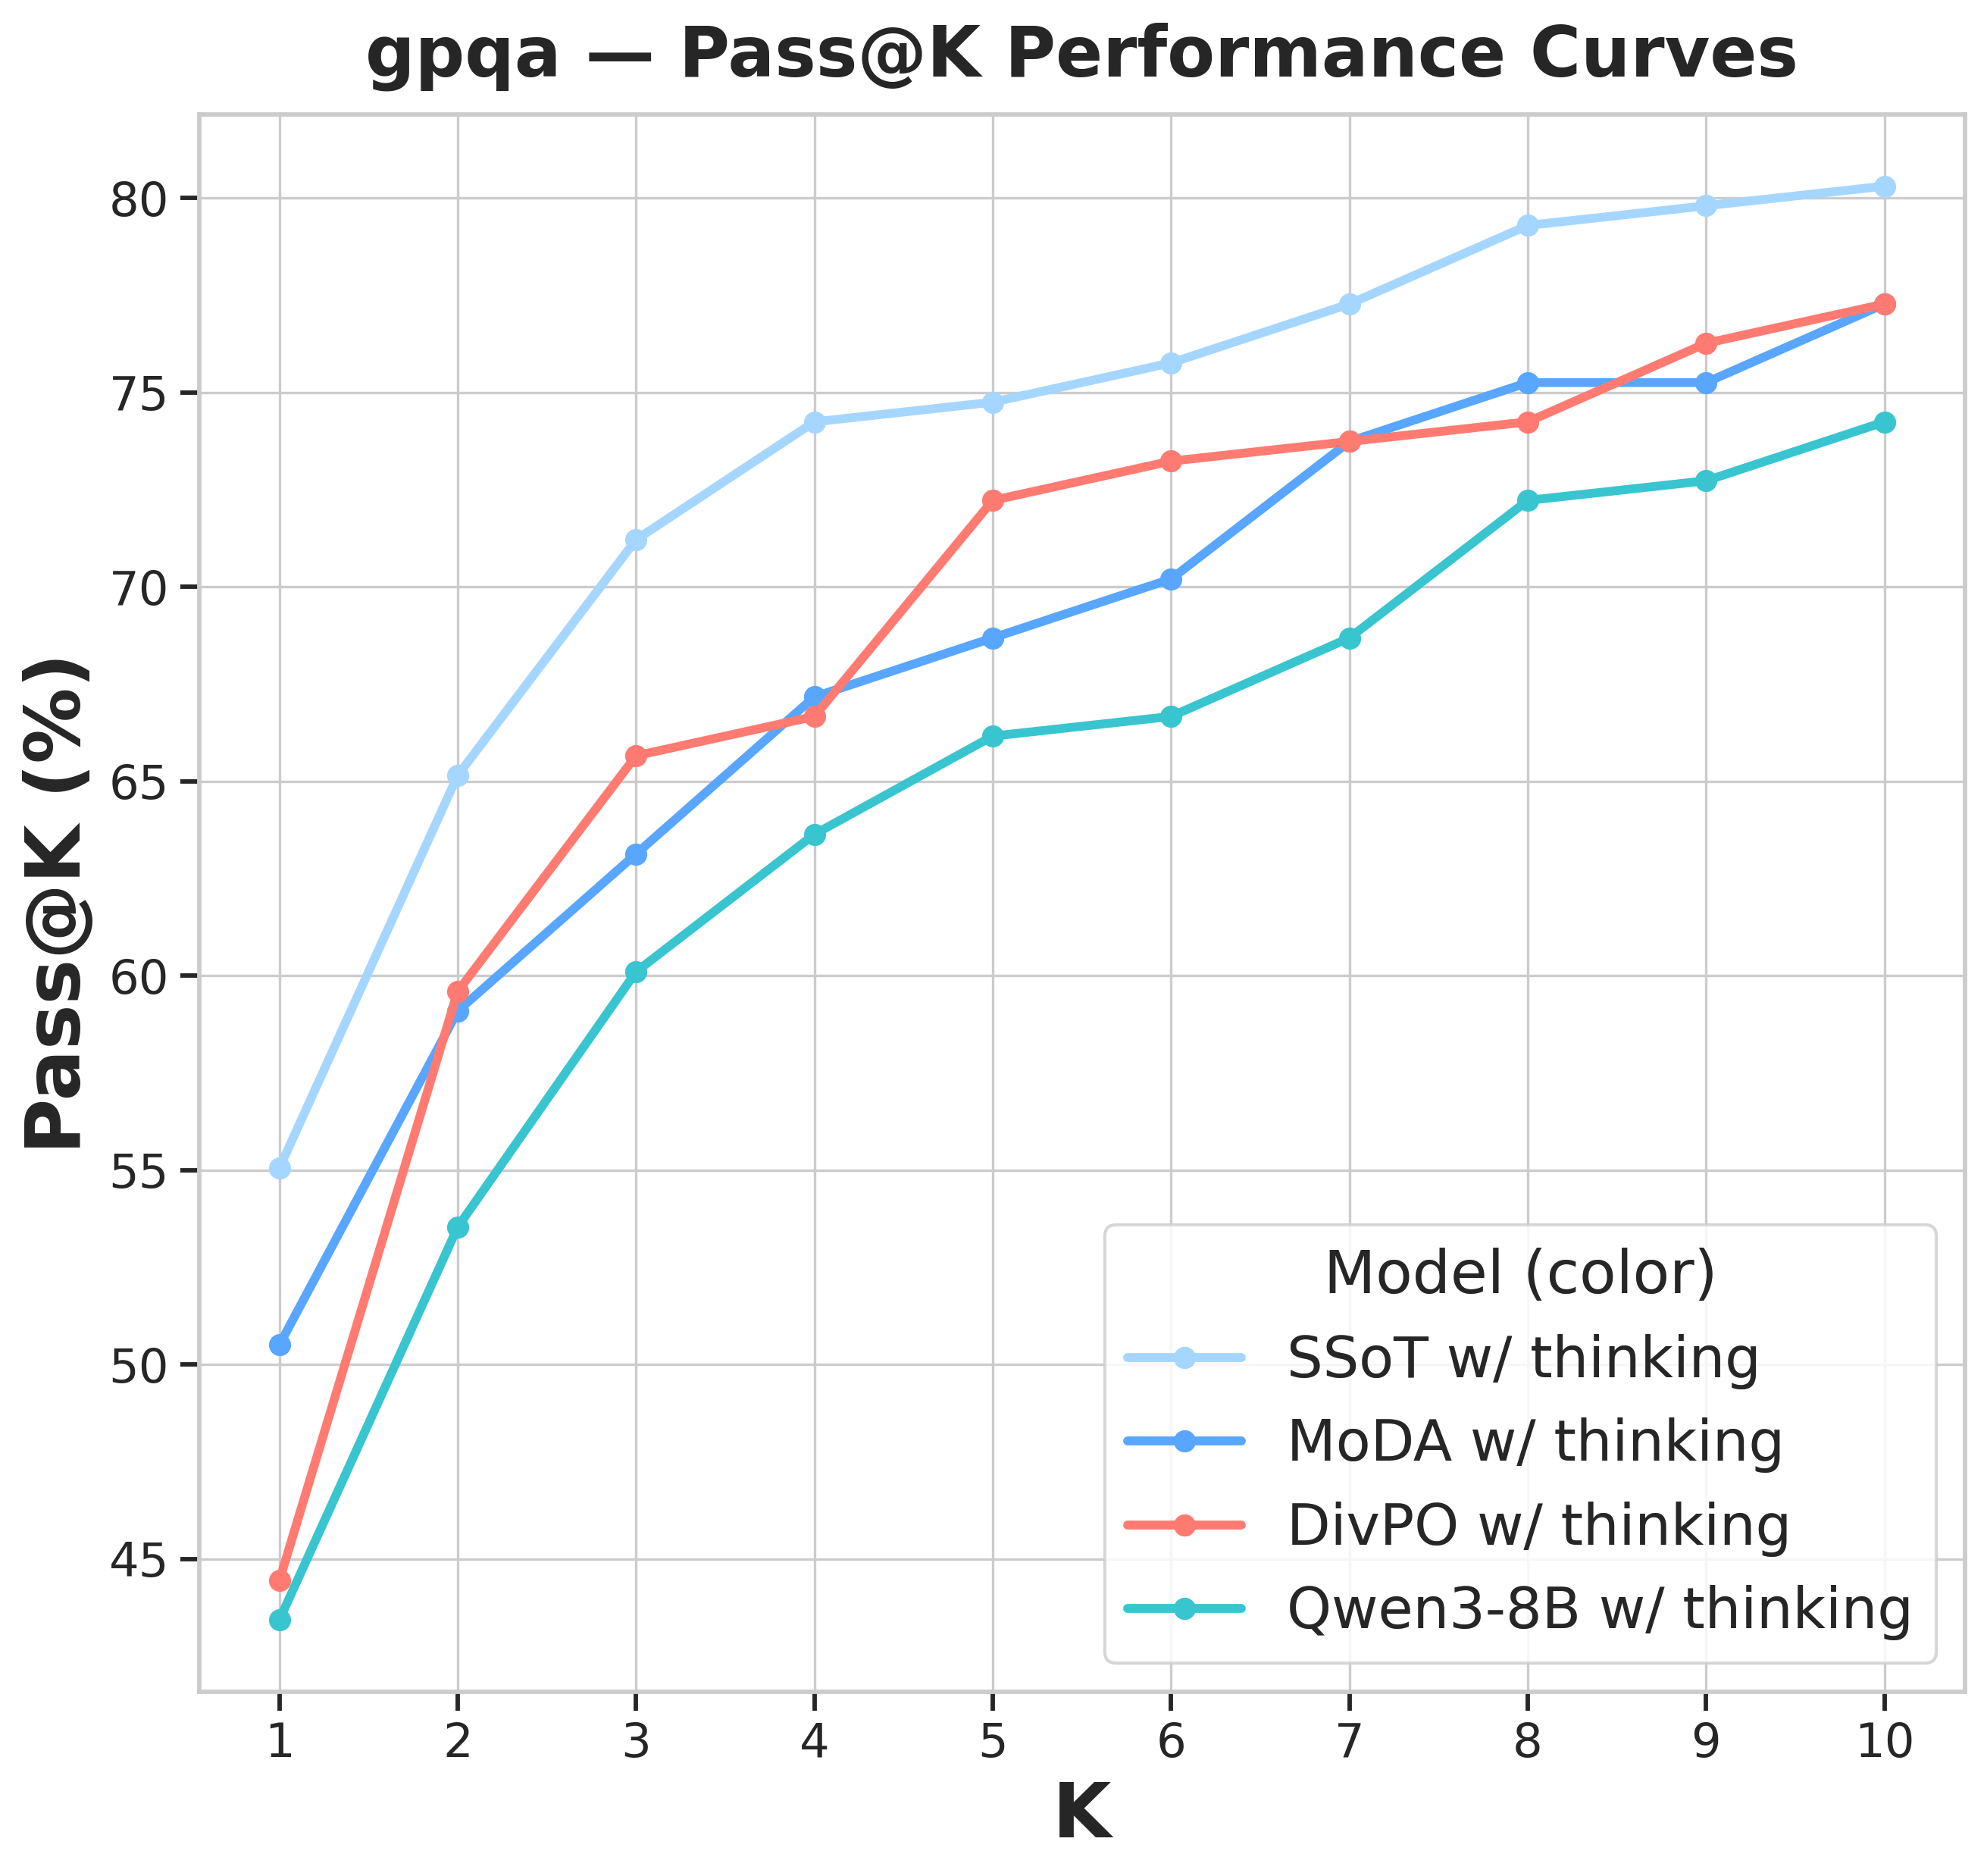
\includegraphics[width=\linewidth]{figures/main_pass_k/pass_at_k_figures/pass_at_k_gpqa_thinking_true.png}
\end{minipage}\hfill
\begin{minipage}{0.24\textwidth}
  \centering
  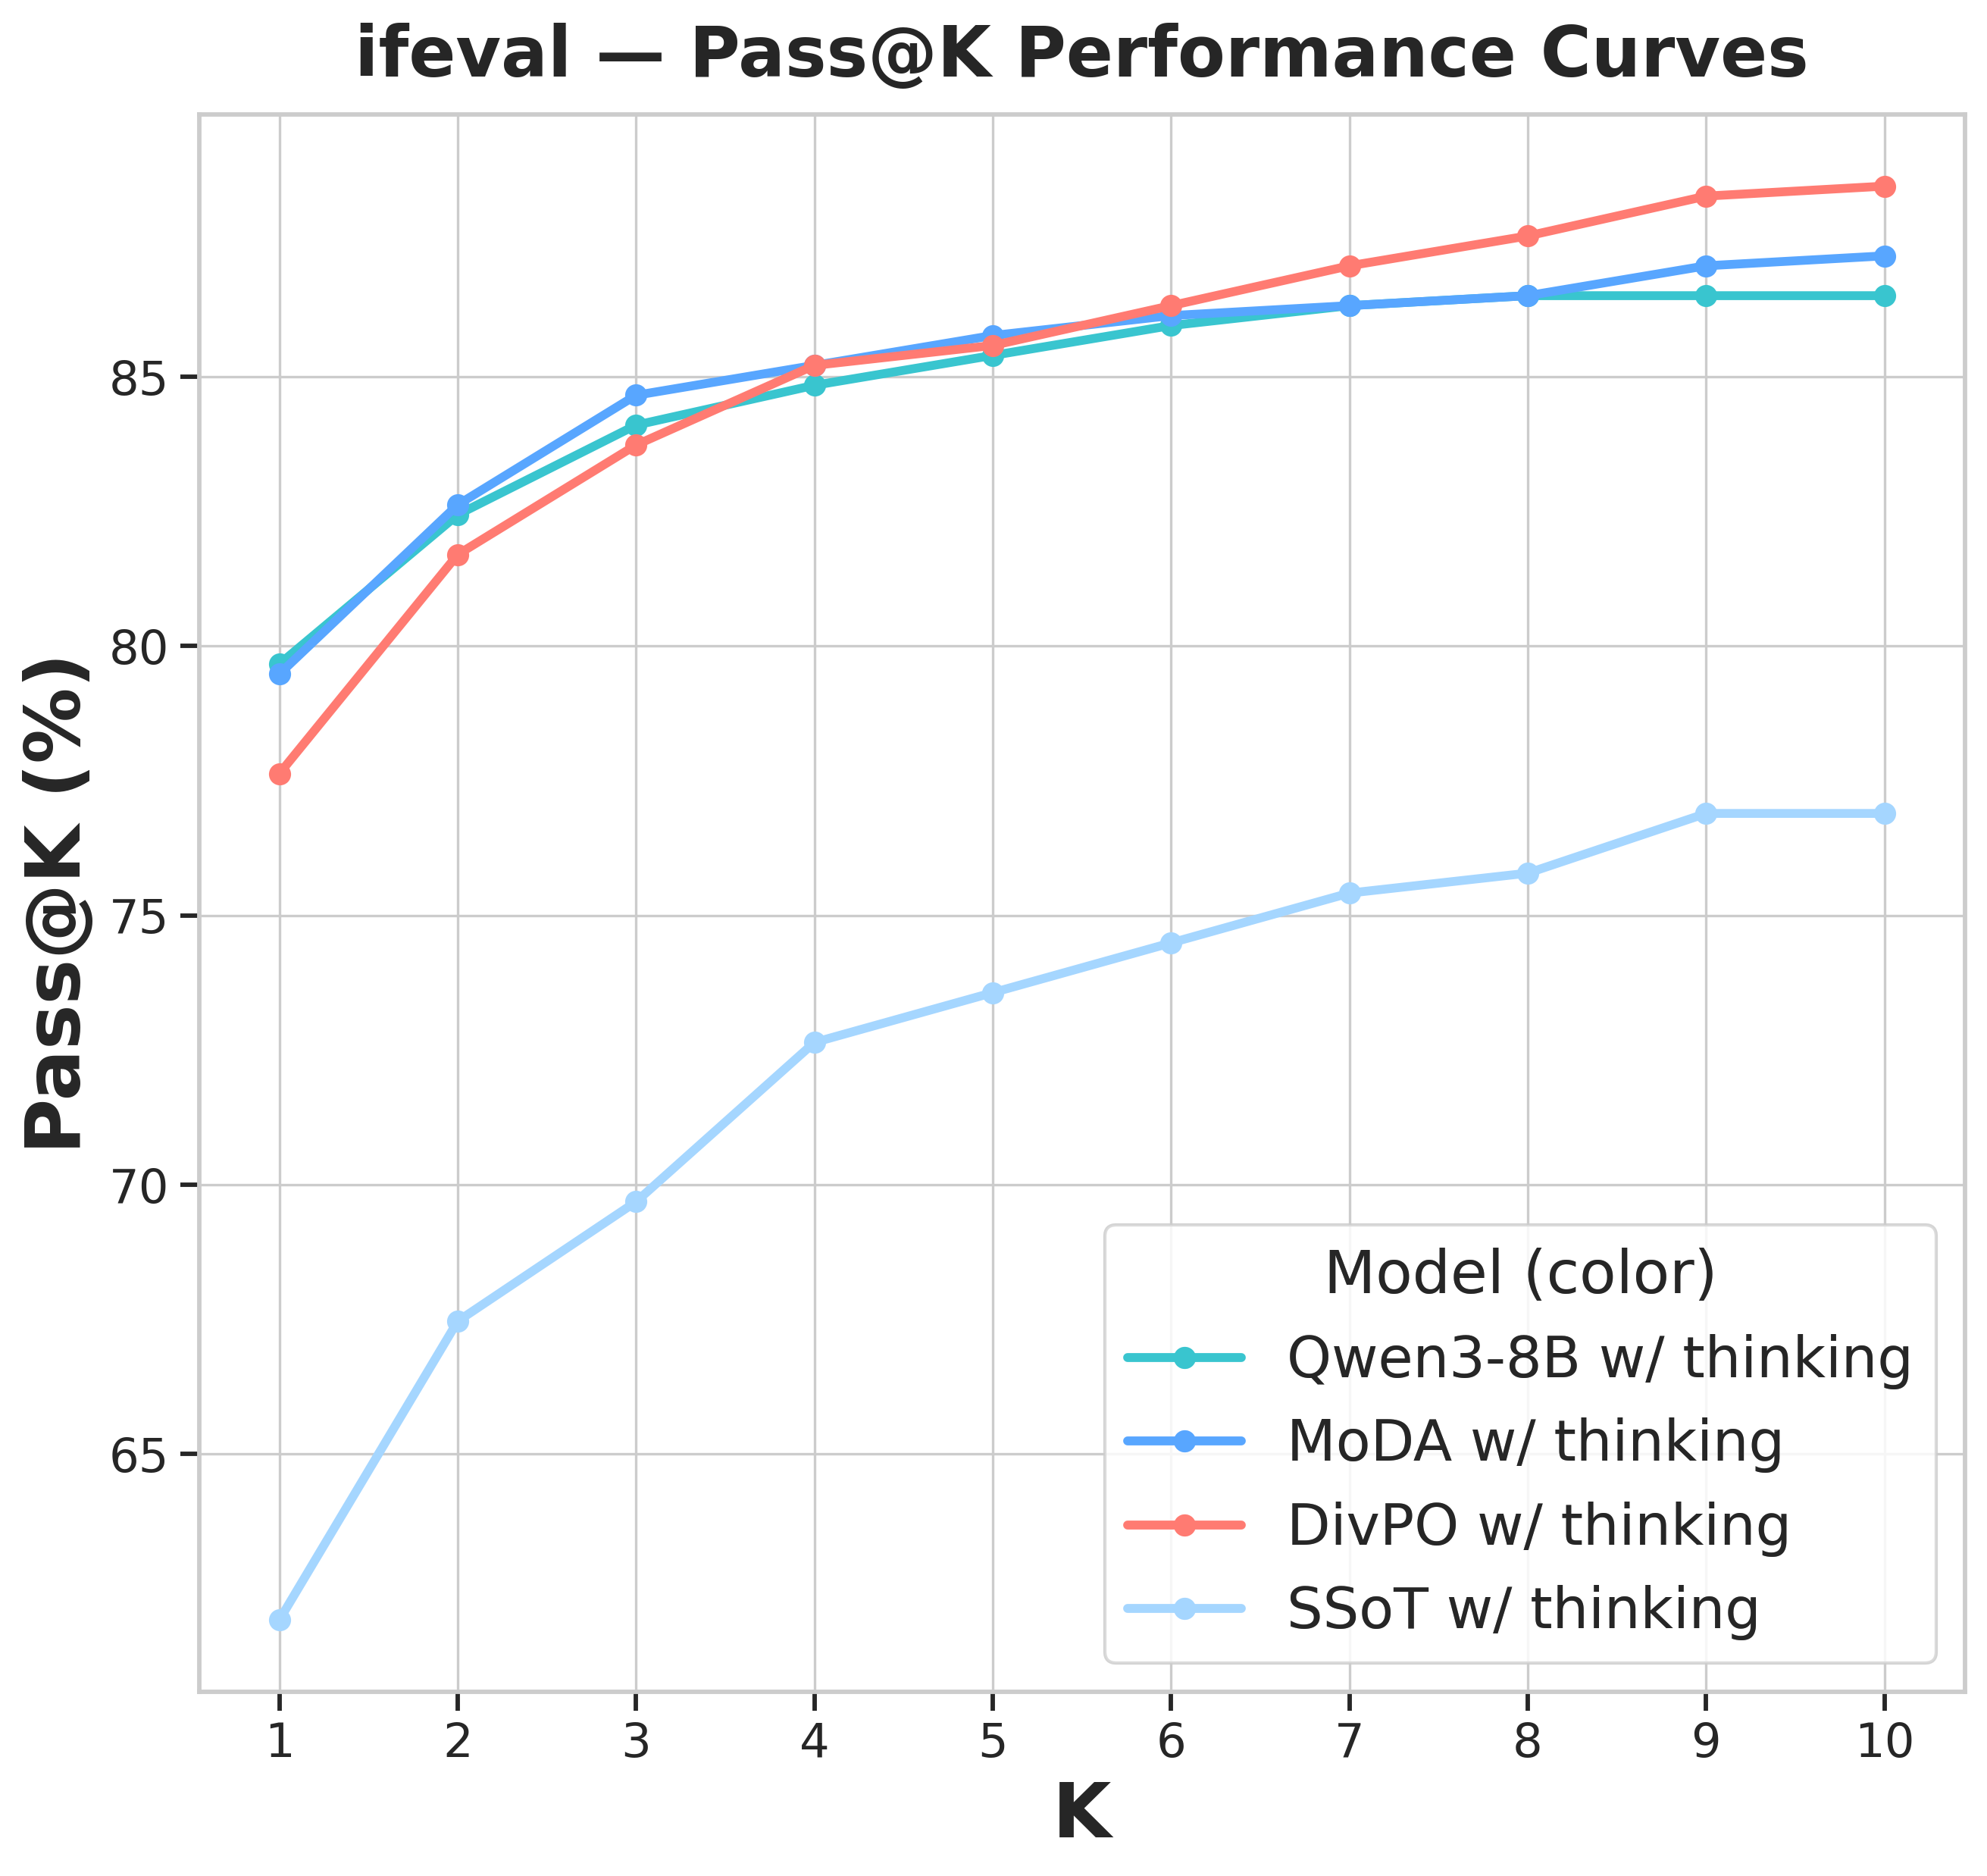
\includegraphics[width=\linewidth]{figures/main_pass_k/pass_at_k_figures/pass_at_k_ifeval_thinking_true.png}
\end{minipage}
\caption{\textbf{General capability retention: pass@k accuracy.} Qwen3-8B base and thinking enabled models.}
\label{fig:general capability pass@k thinking enabled}
\end{figure}


\begin{figure}[H]
\begin{minipage}{0.24\textwidth}
  \centering
  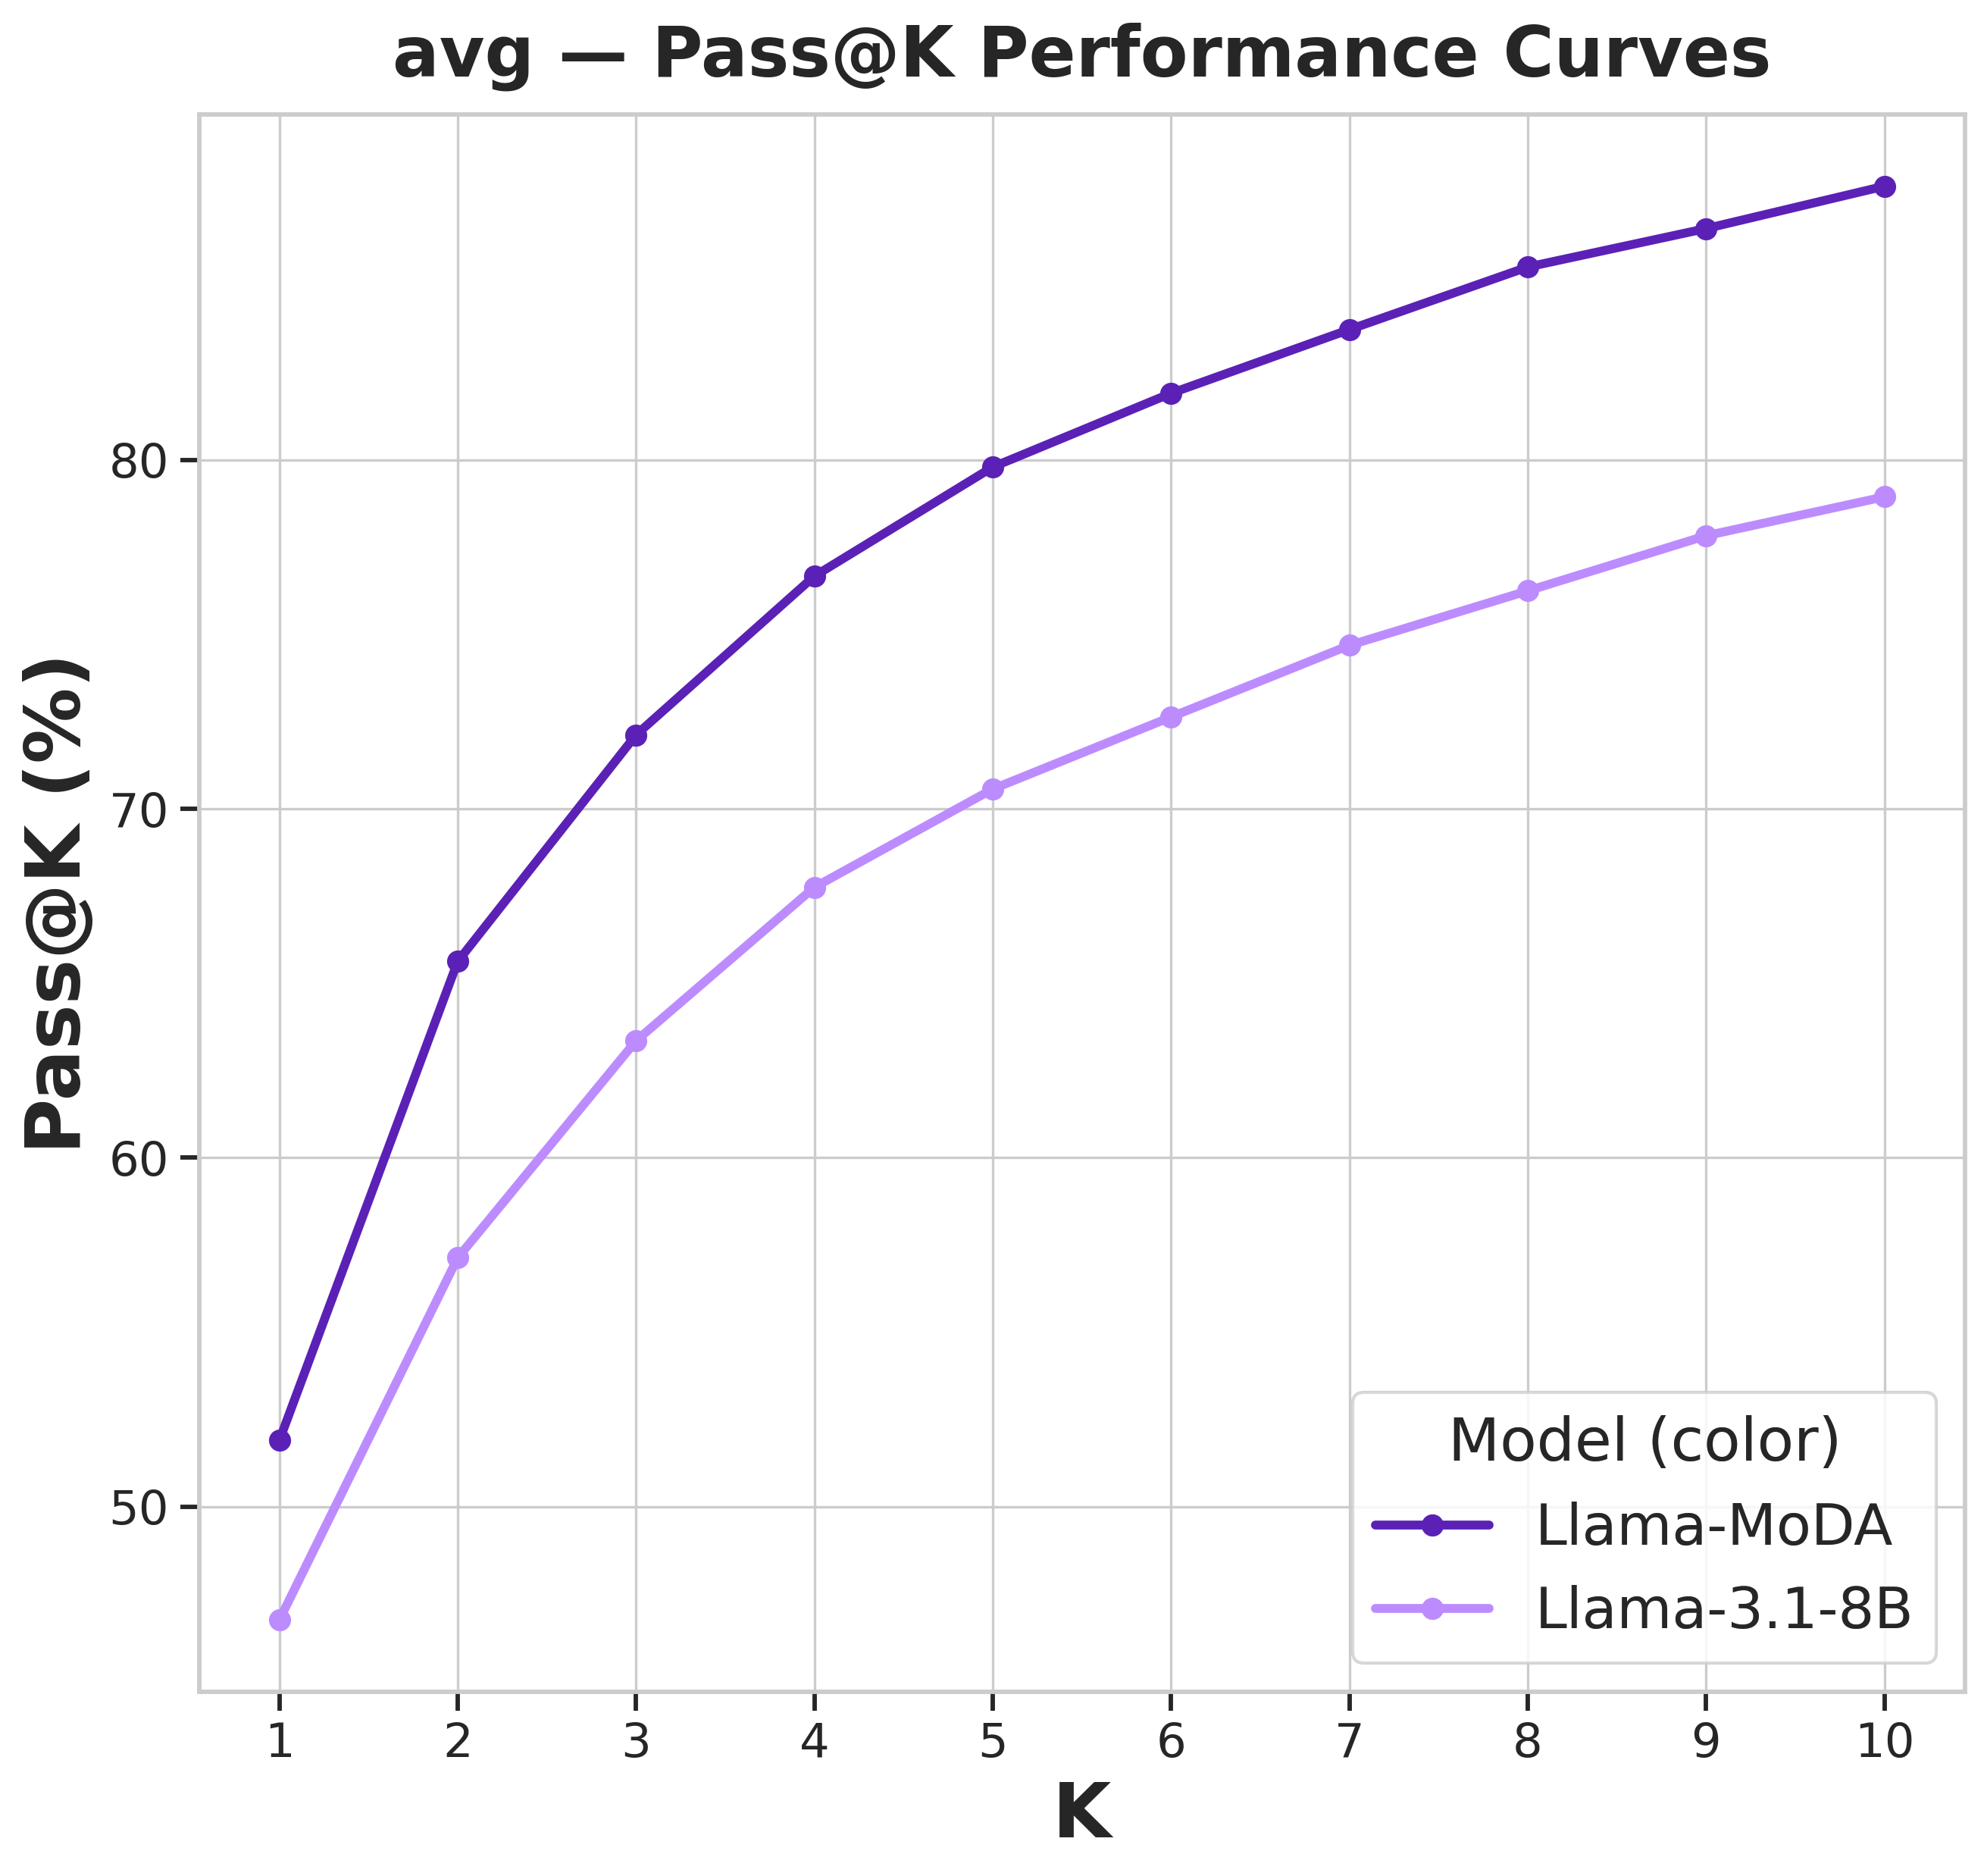
\includegraphics[width=\linewidth]{figures/main_pass_k/pass_at_k_figures/pass_at_k_avg_thinking_false_base_model_llama3_1-8b.png}
\end{minipage}\hfill
\centering
\begin{minipage}{0.24\textwidth}
  \centering
  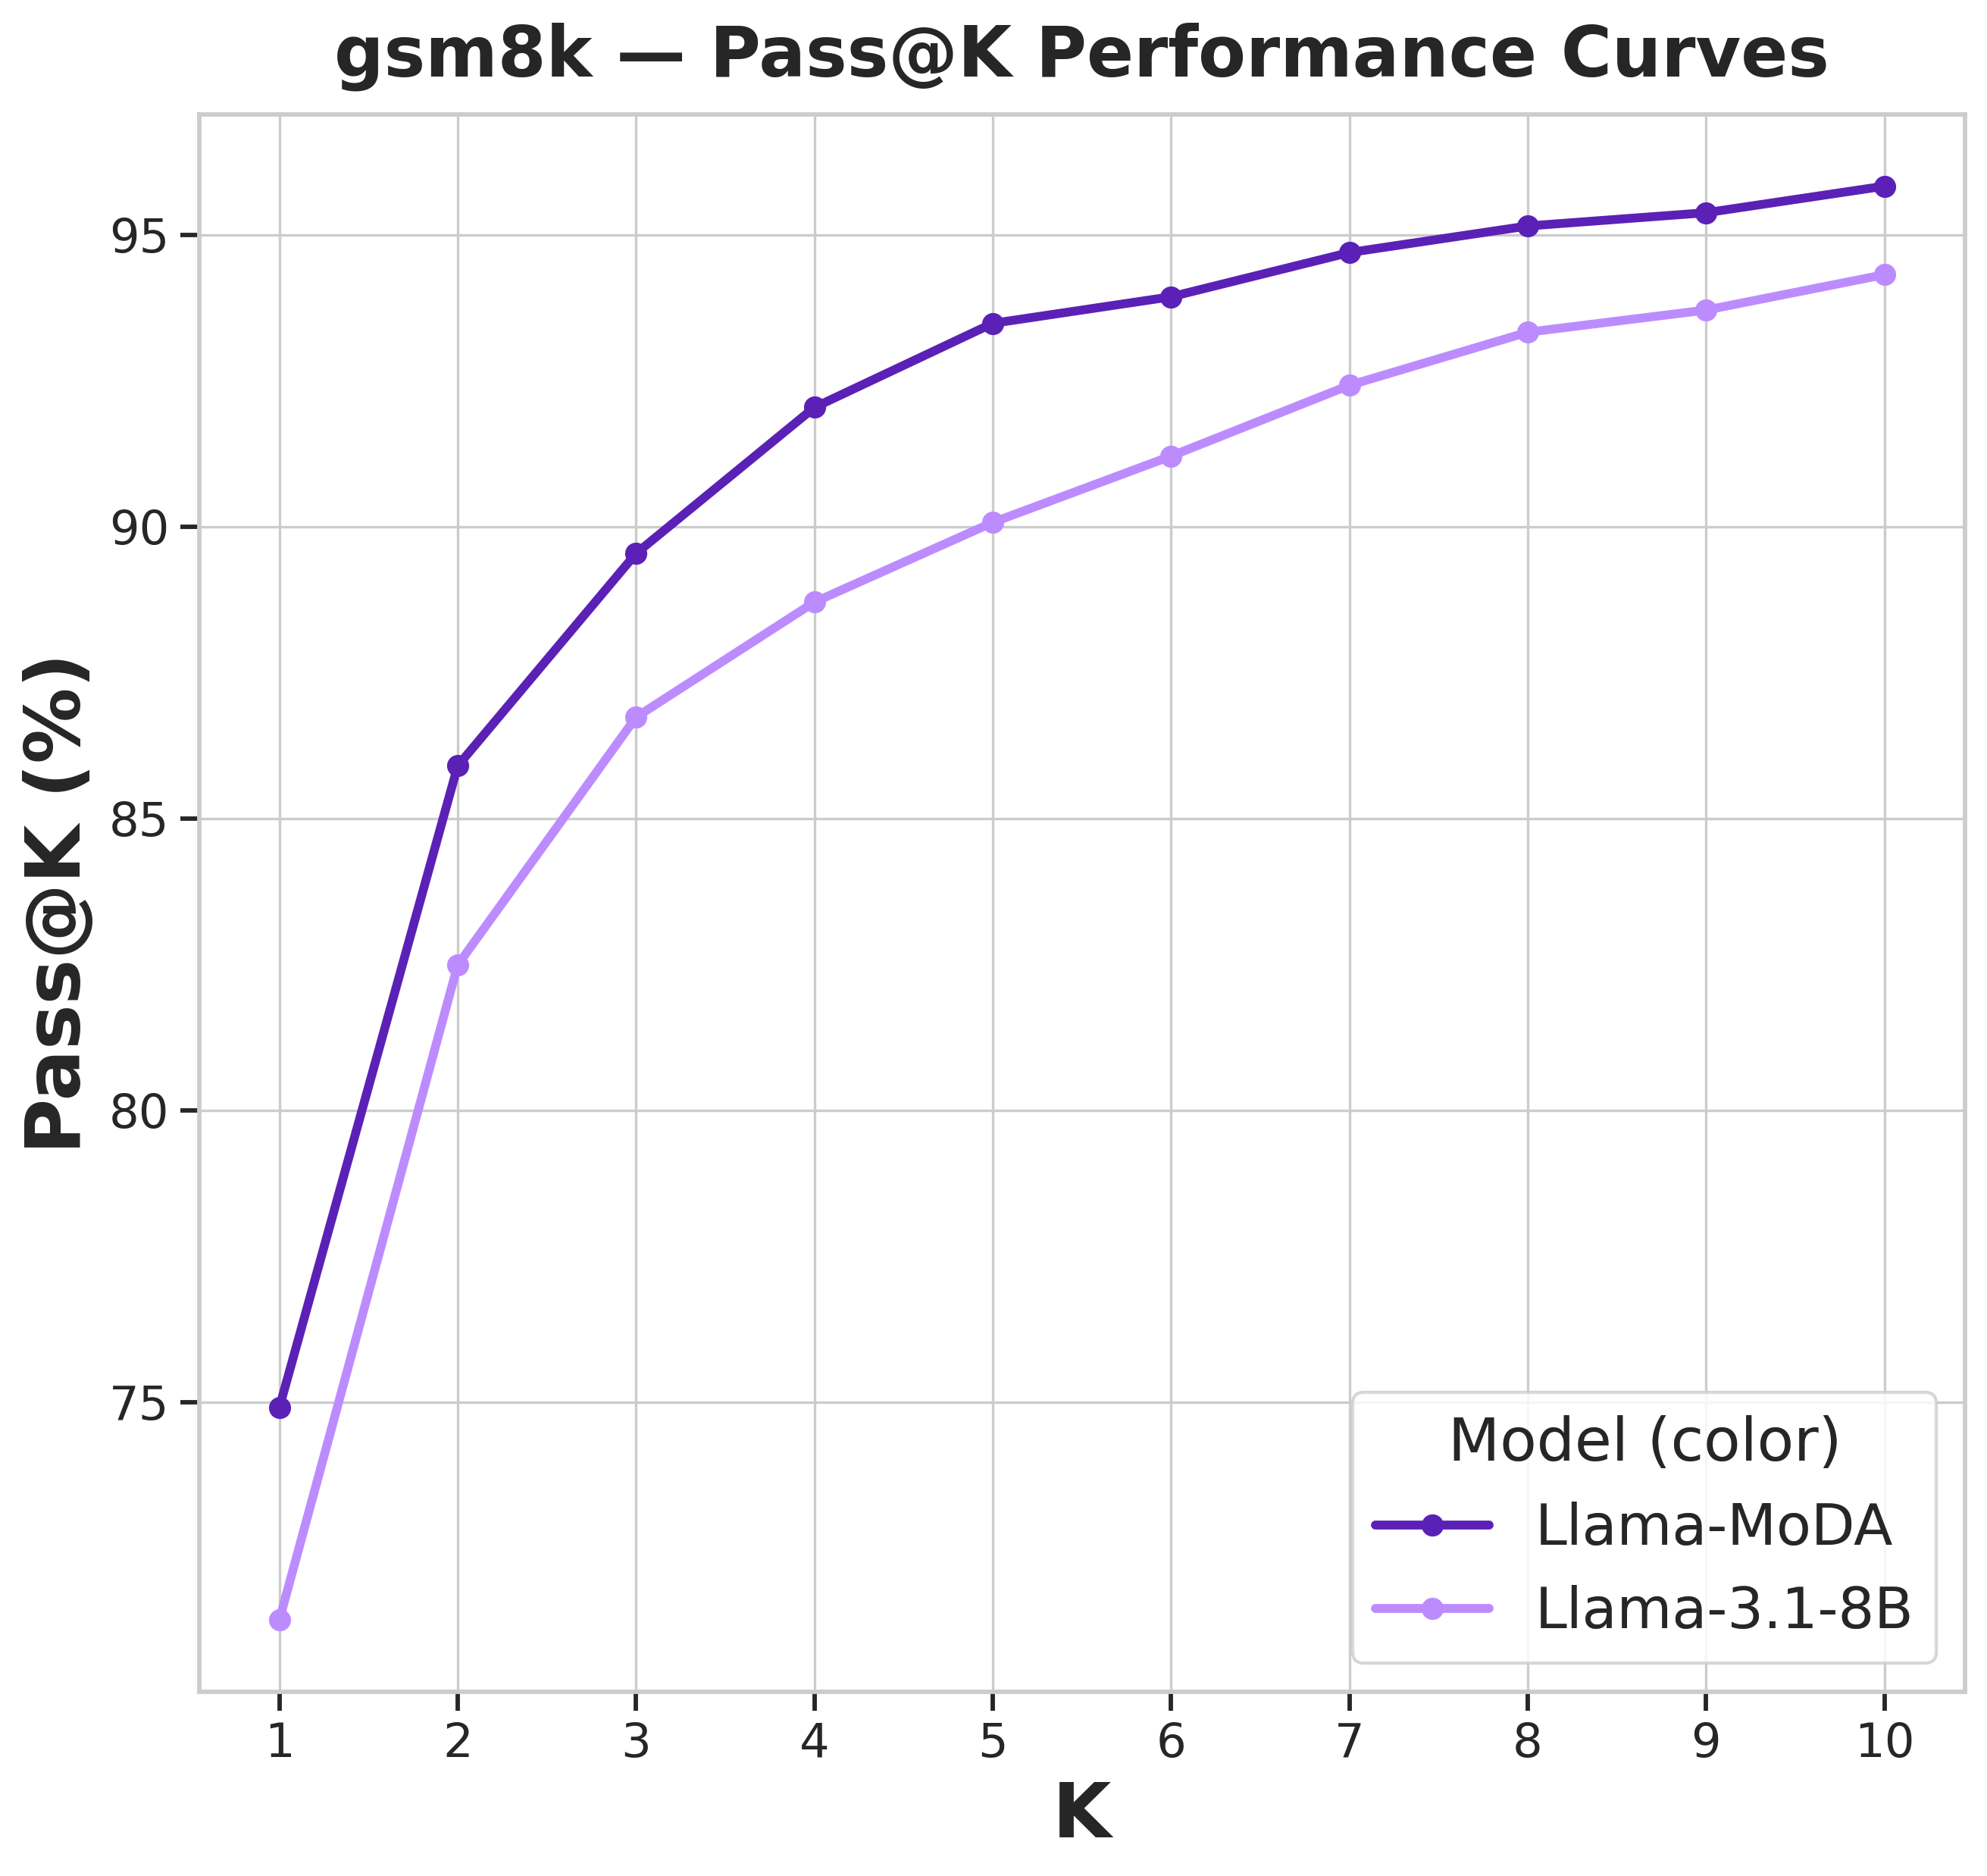
\includegraphics[width=\linewidth]{figures/main_pass_k/pass_at_k_figures/pass_at_k_gsm8k_thinking_false_base_model_llama3_1-8b.png}
\end{minipage}\hfill
\begin{minipage}{0.24\textwidth}
  \centering
  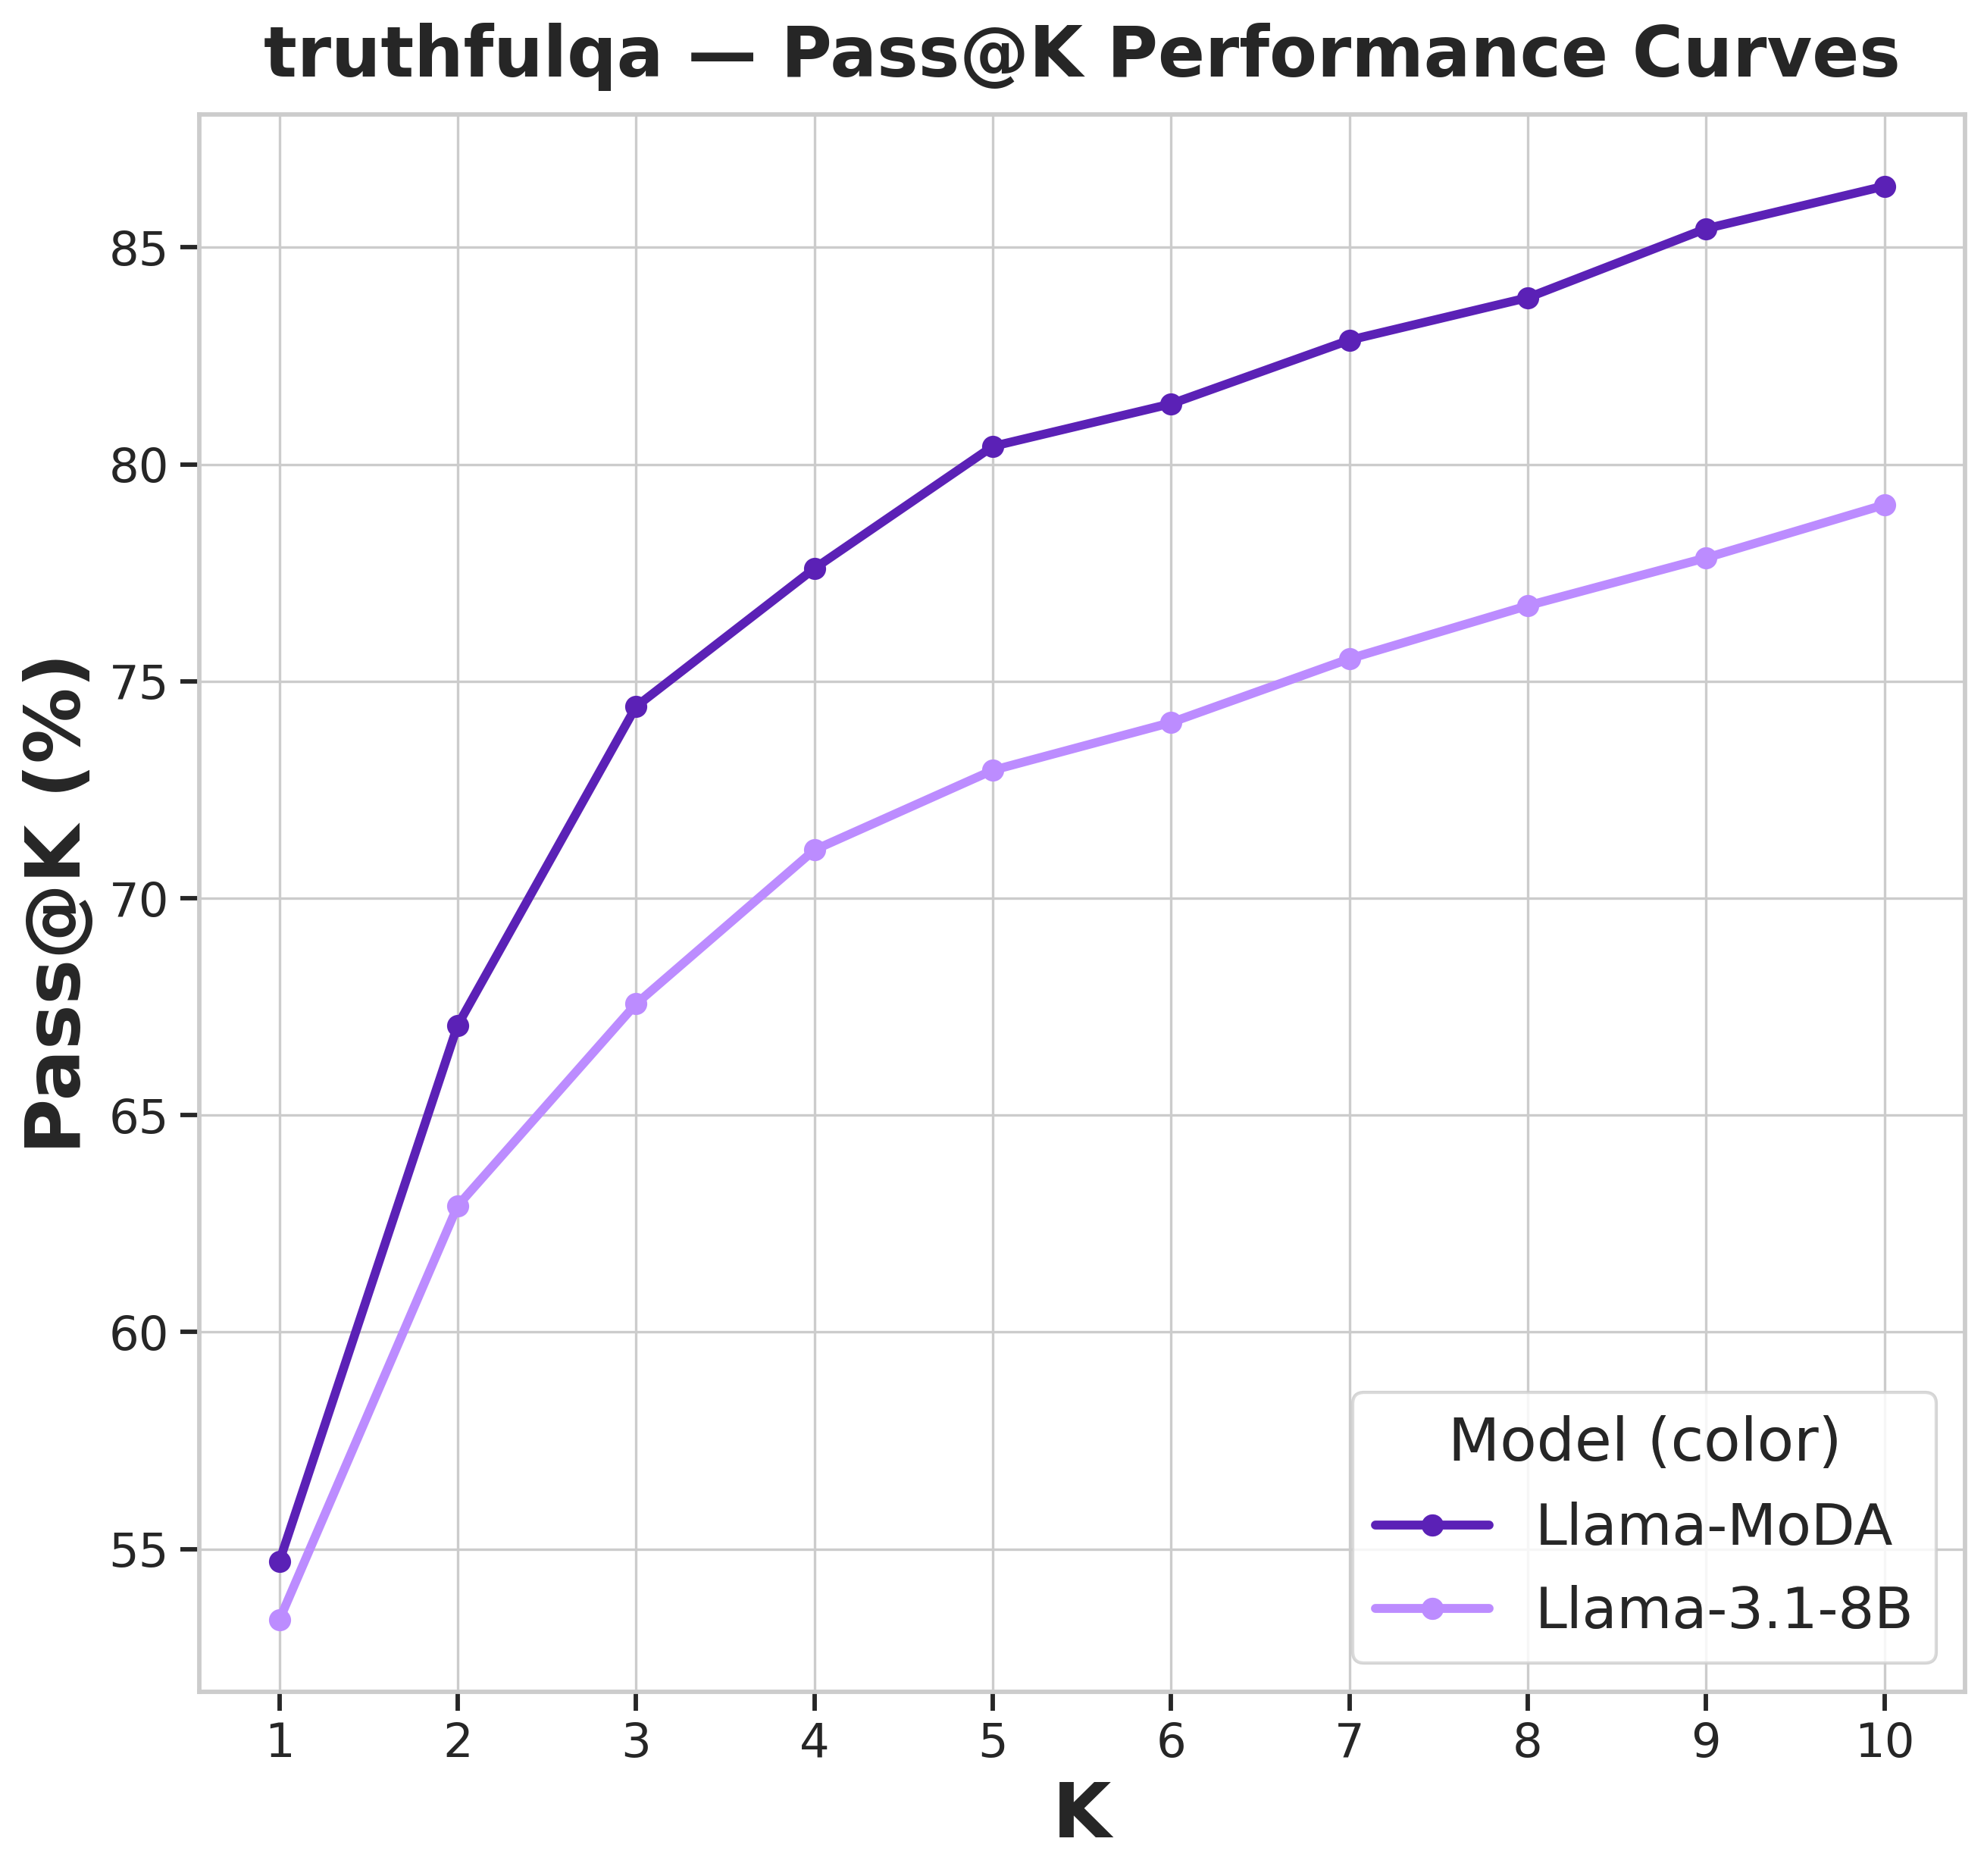
\includegraphics[width=\linewidth]{figures/main_pass_k/pass_at_k_figures/pass_at_k_truthfulqa_thinking_false_base_model_llama3_1-8b.png}
\end{minipage}\hfill
\begin{minipage}{0.24\textwidth}
  \centering
  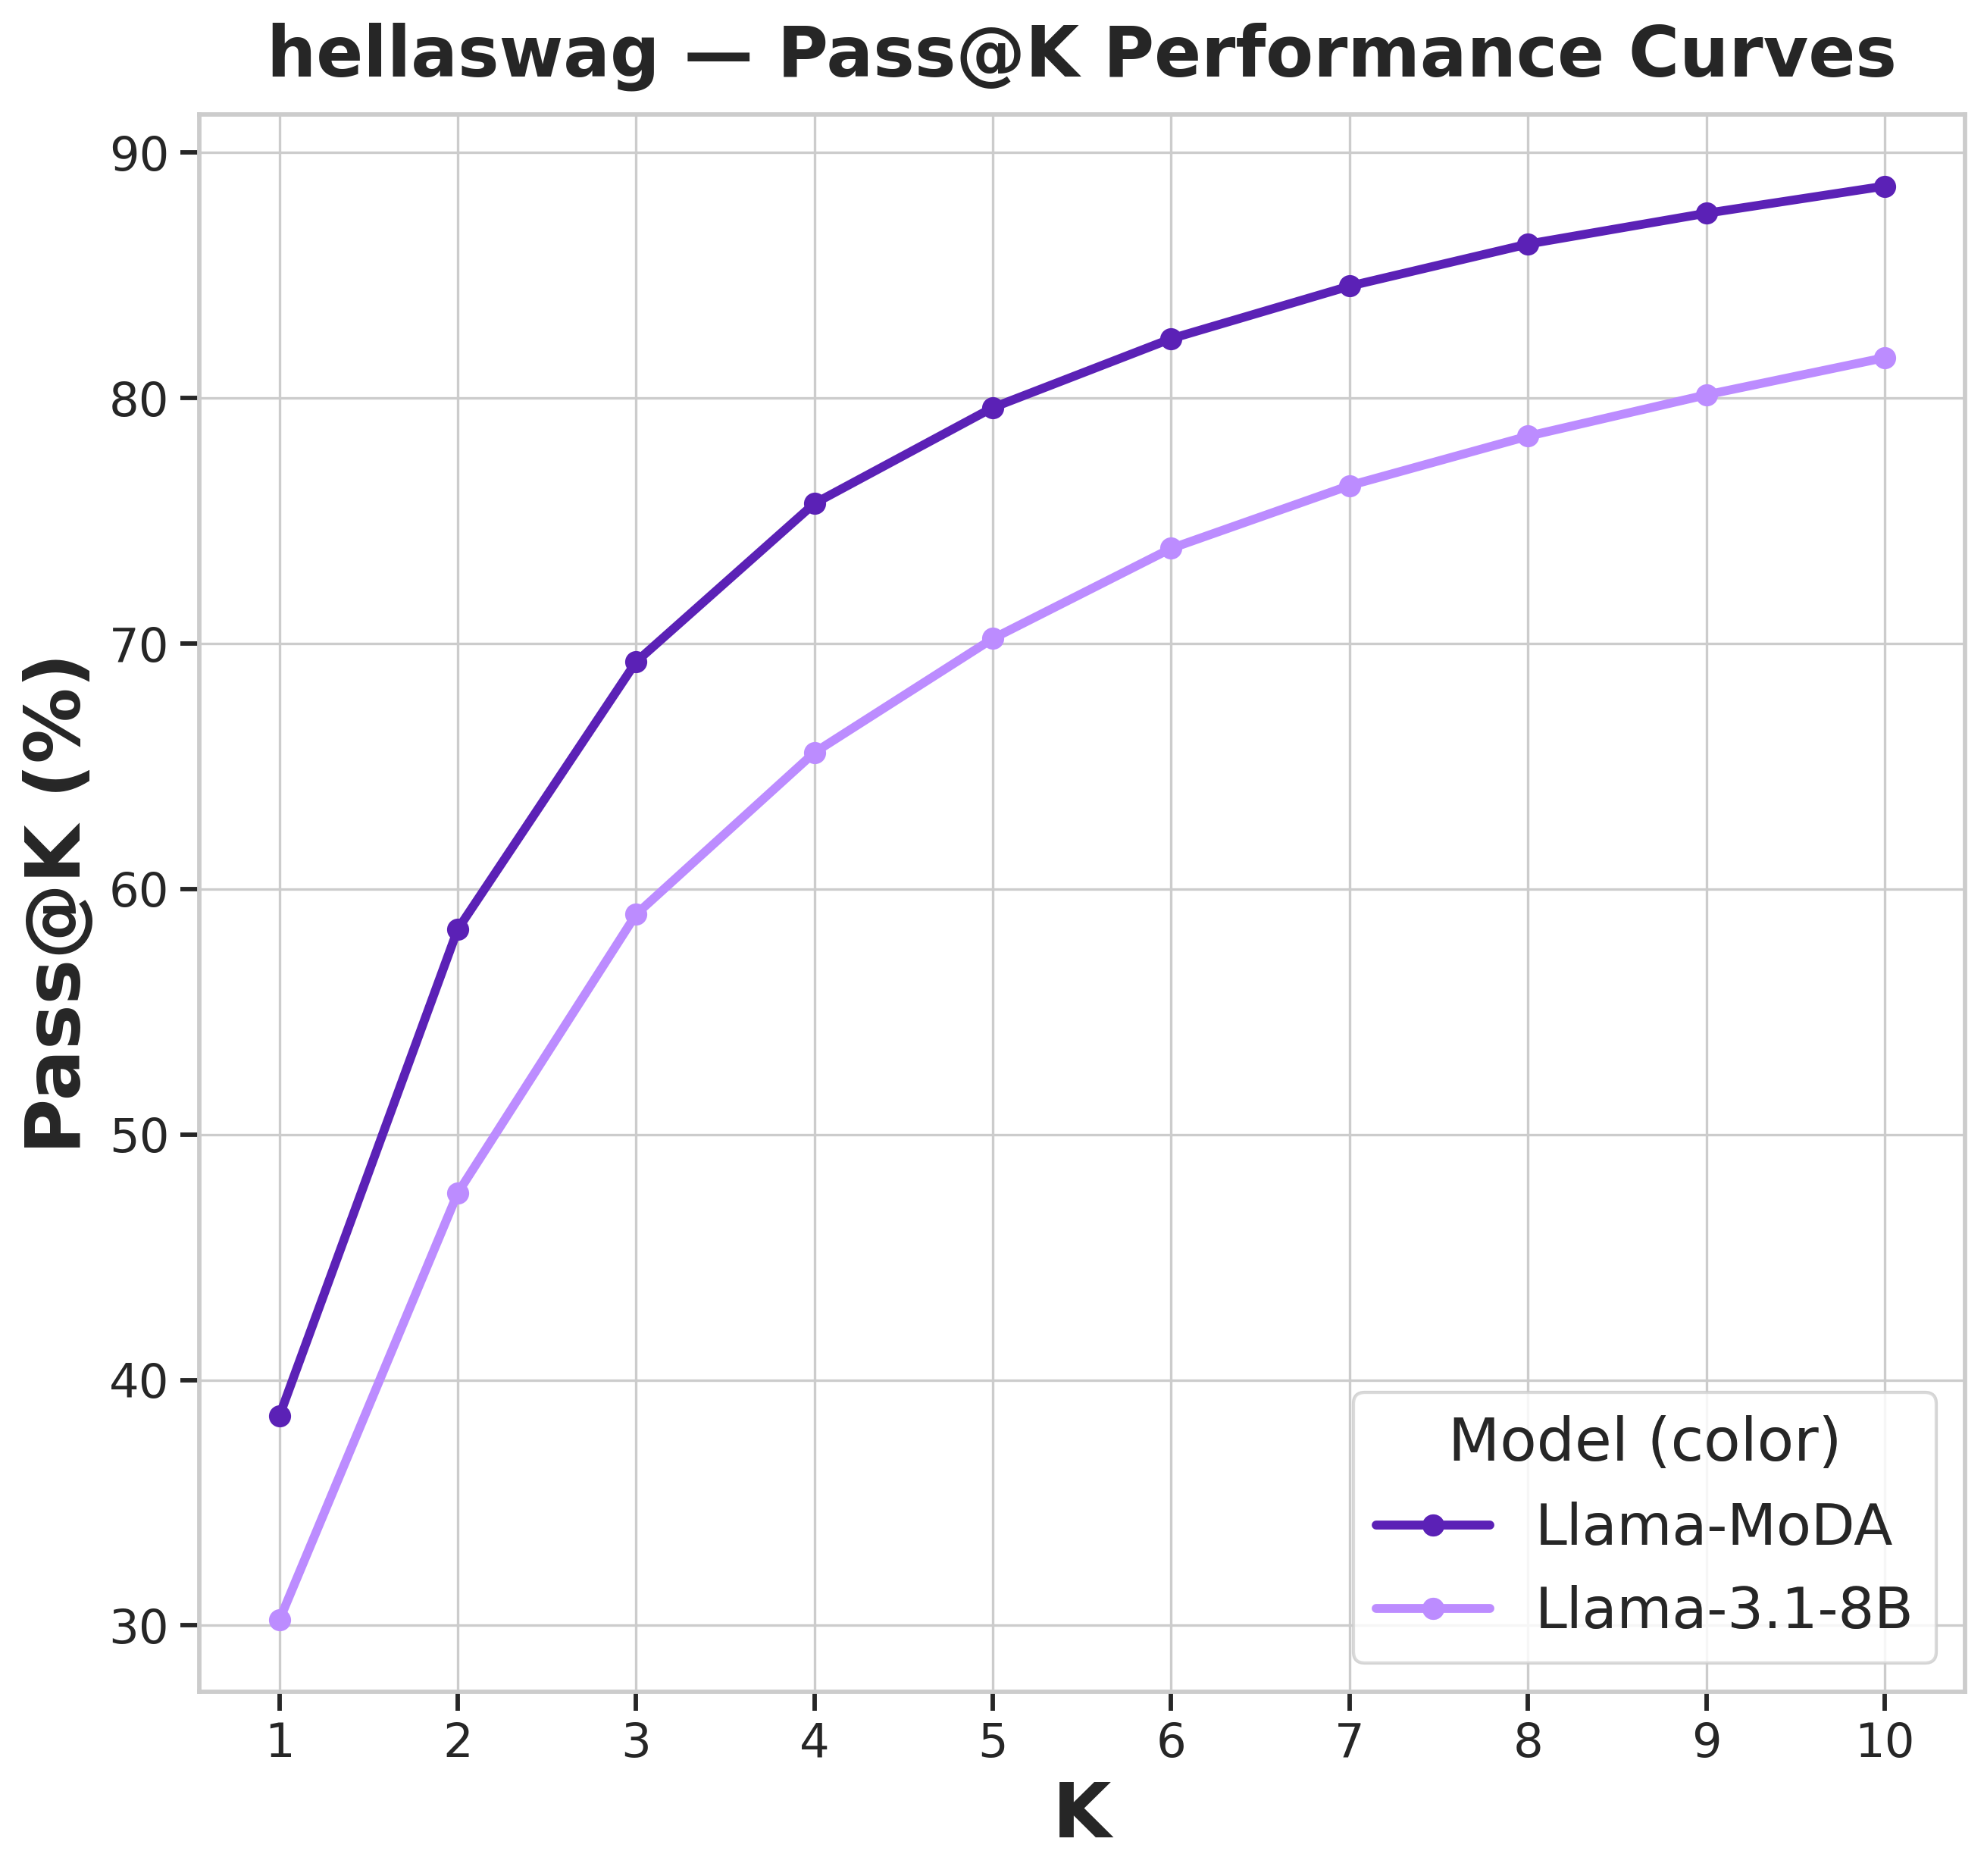
\includegraphics[width=\linewidth]{figures/main_pass_k/pass_at_k_figures/pass_at_k_hellaswag_thinking_false_base_model_llama3_1-8b.png}
\end{minipage}
\centering
\begin{minipage}{0.24\textwidth}
  \centering
  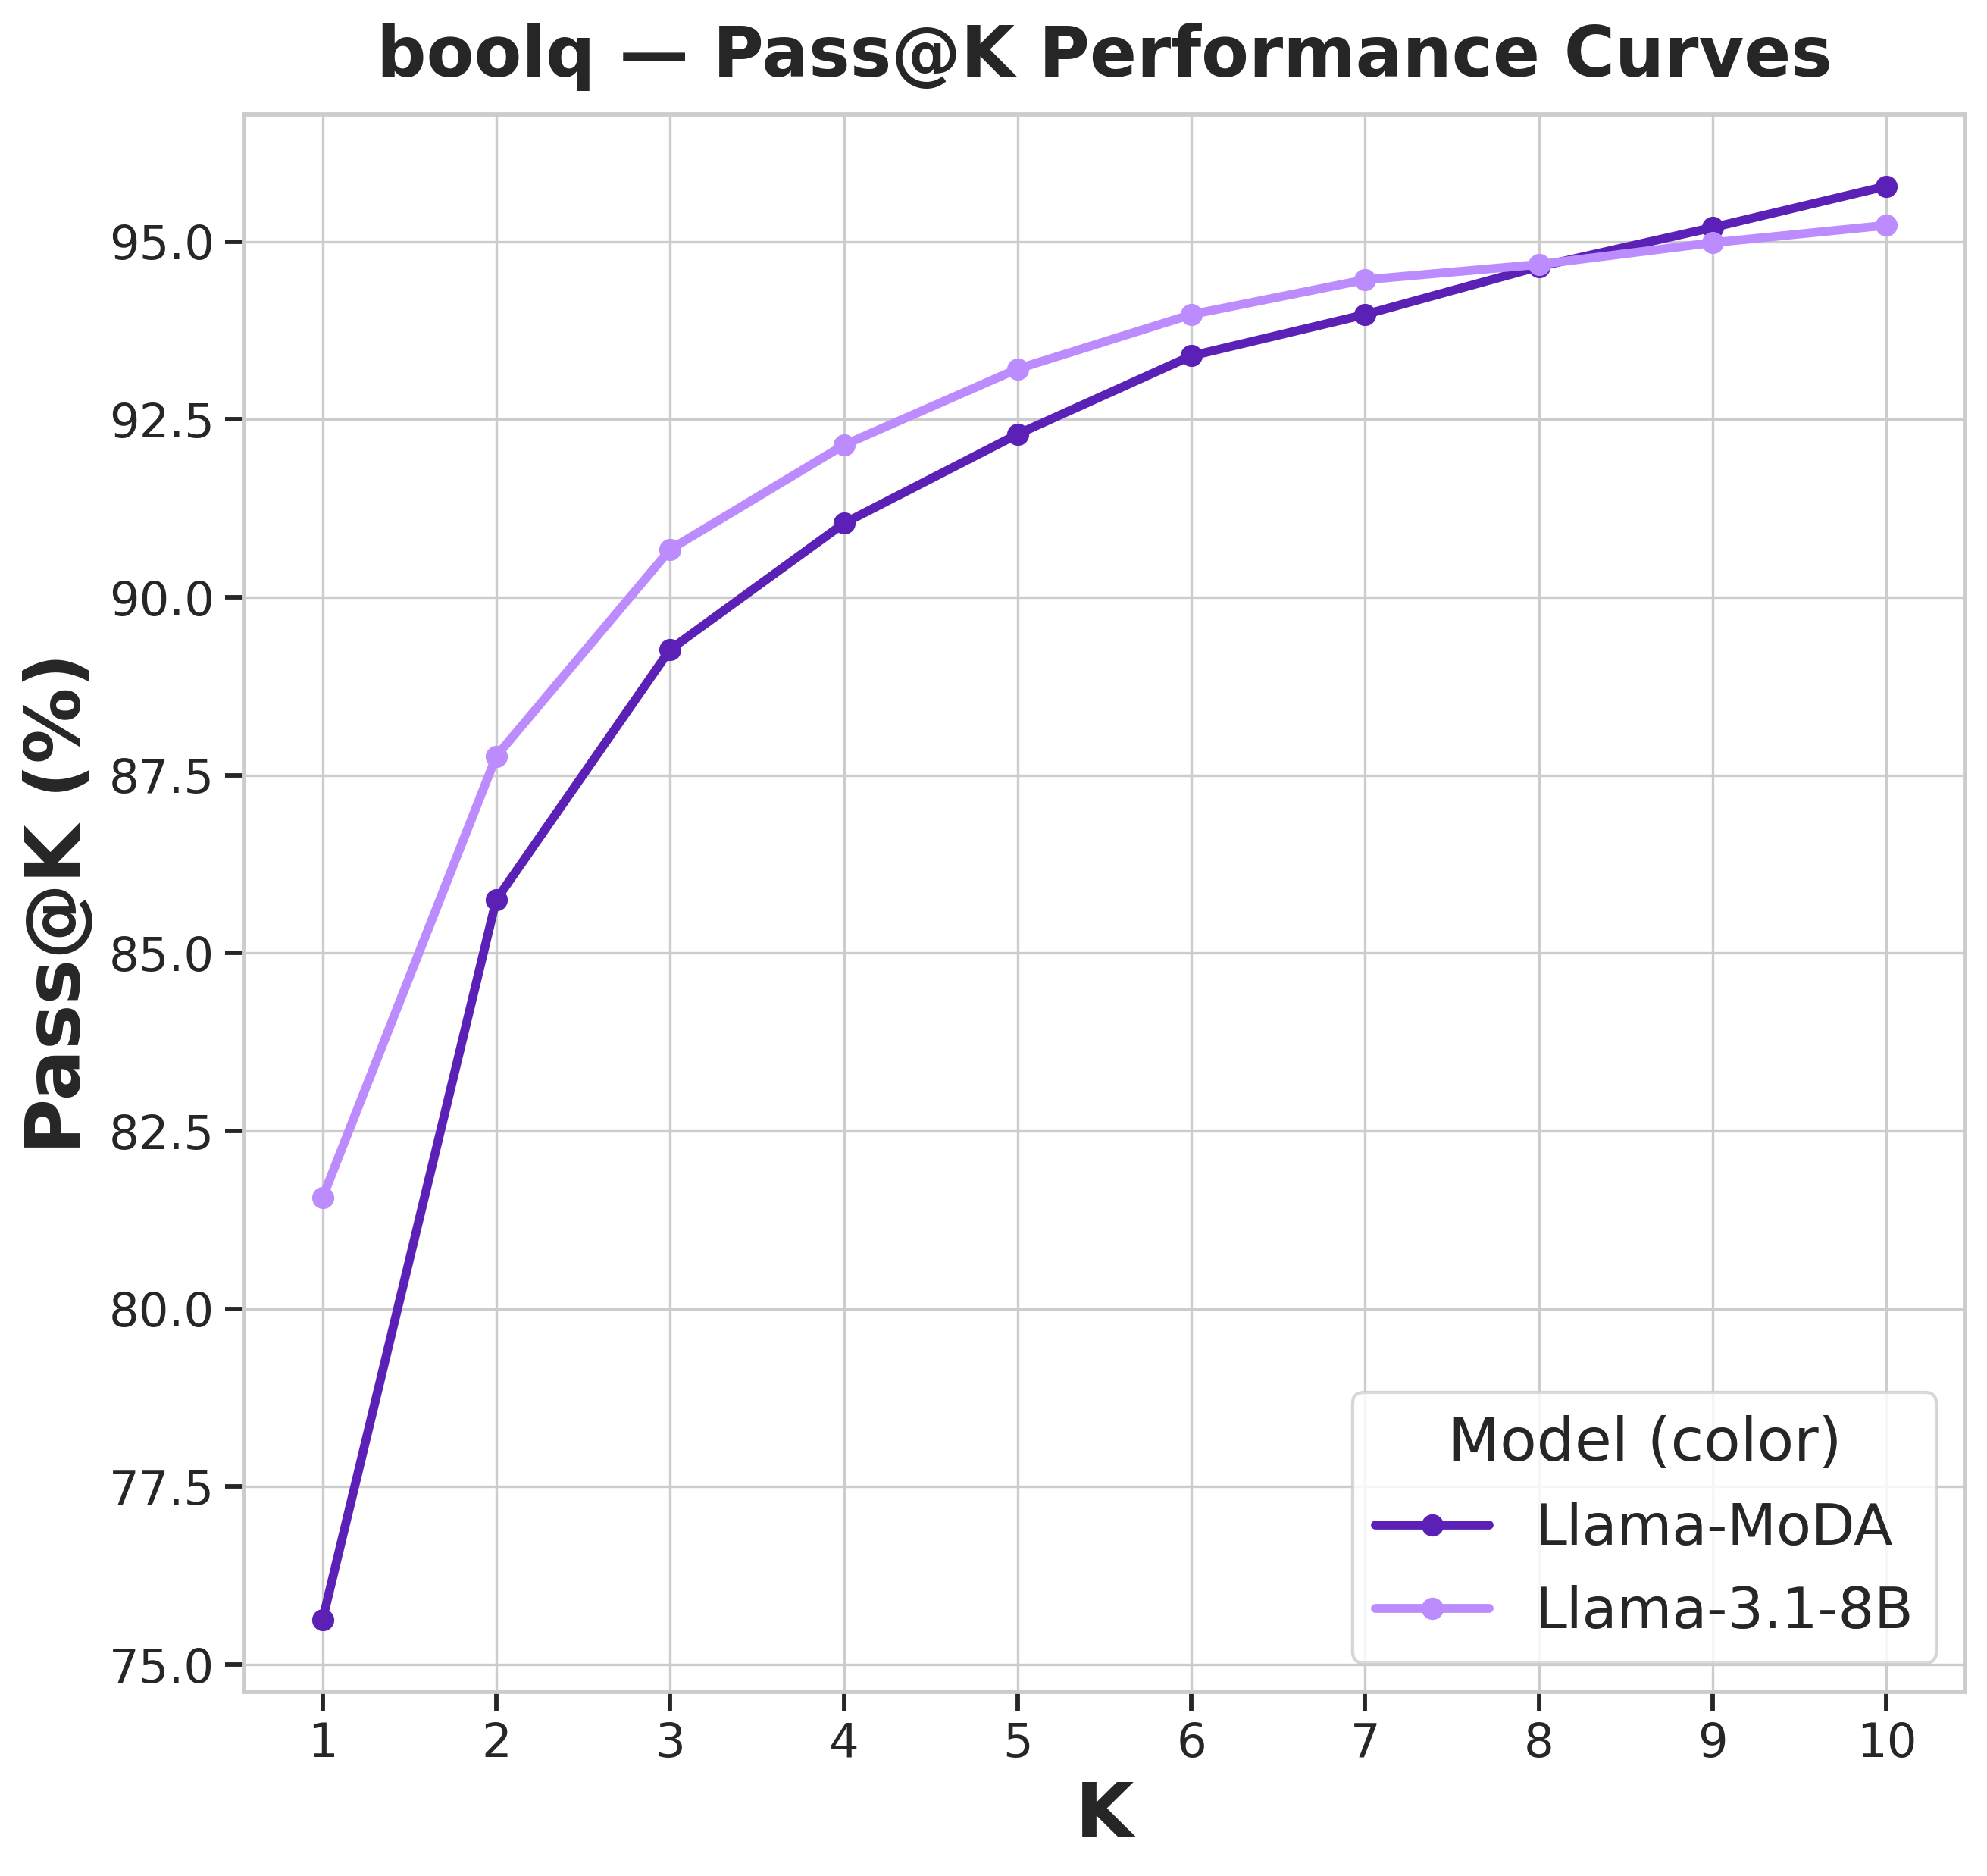
\includegraphics[width=\linewidth]{figures/main_pass_k/pass_at_k_figures/pass_at_k_boolq_thinking_false_base_model_llama3_1-8b.png}
\end{minipage}\hfill
\centering
\begin{minipage}{0.24\textwidth}
  \centering
  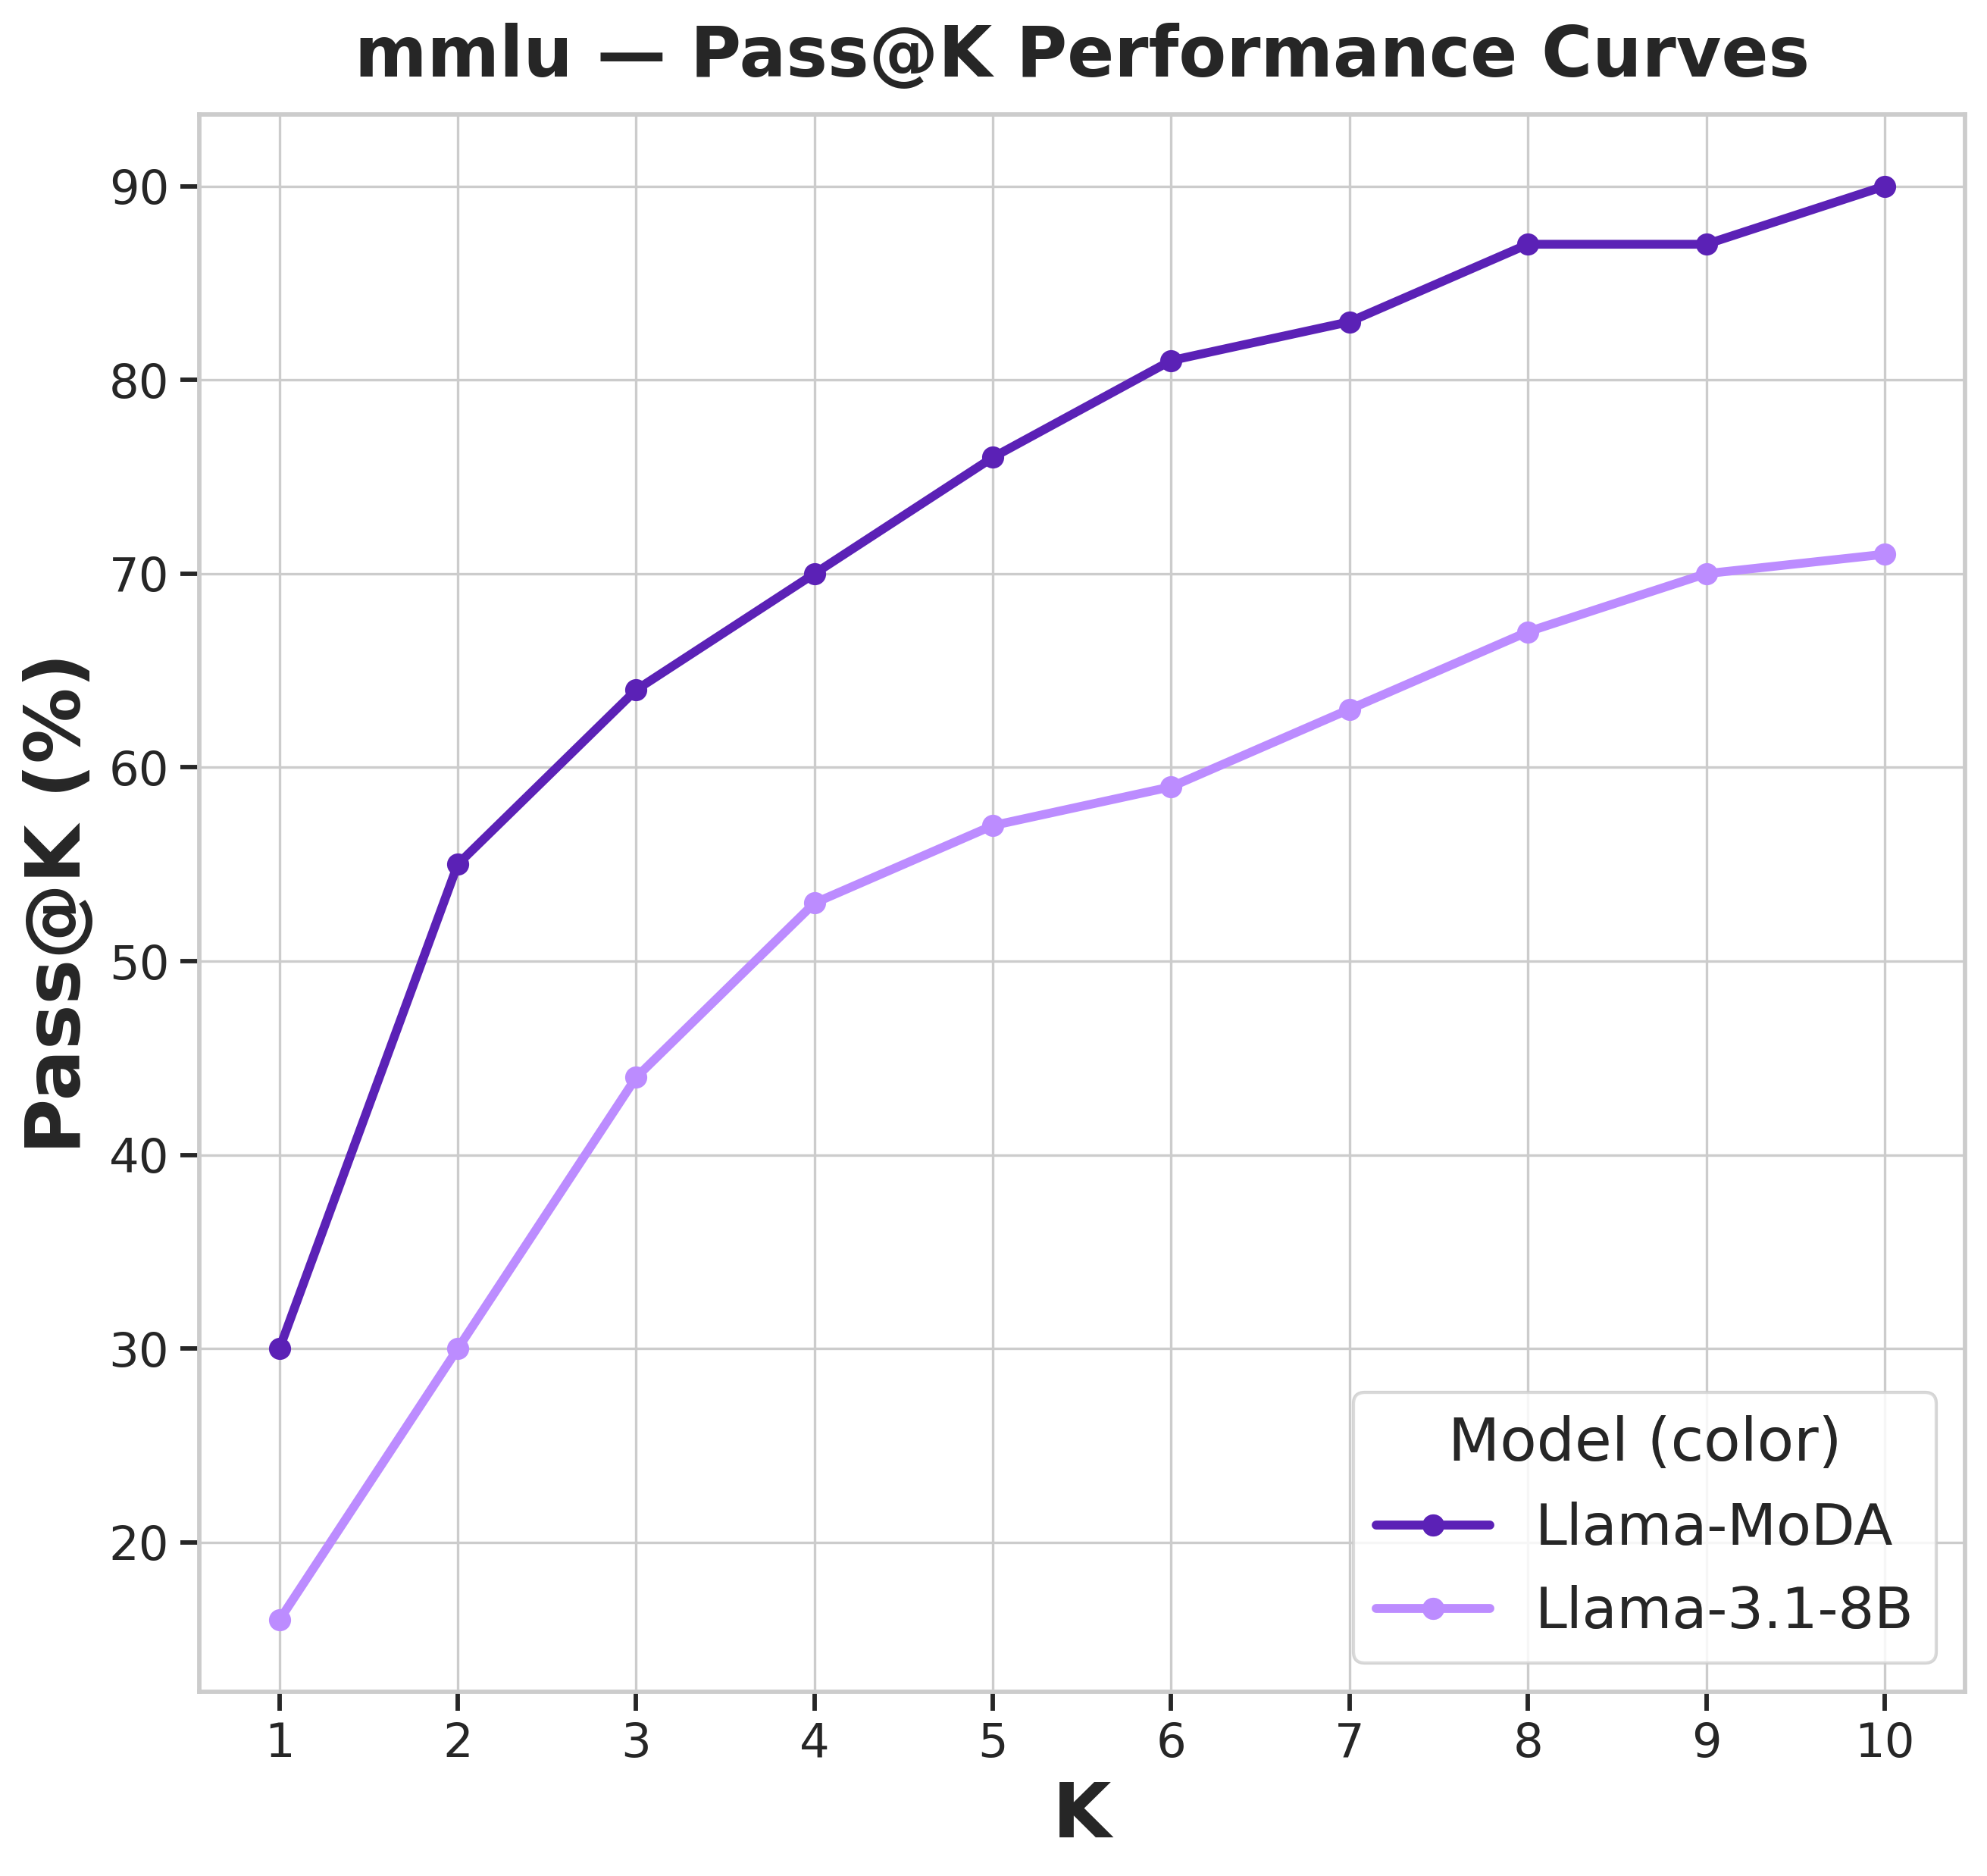
\includegraphics[width=\linewidth]{figures/main_pass_k/pass_at_k_figures/pass_at_k_mmlu_thinking_false_base_model_llama3_1-8b.png}
\end{minipage}\hfill
\begin{minipage}{0.24\textwidth}
  \centering
  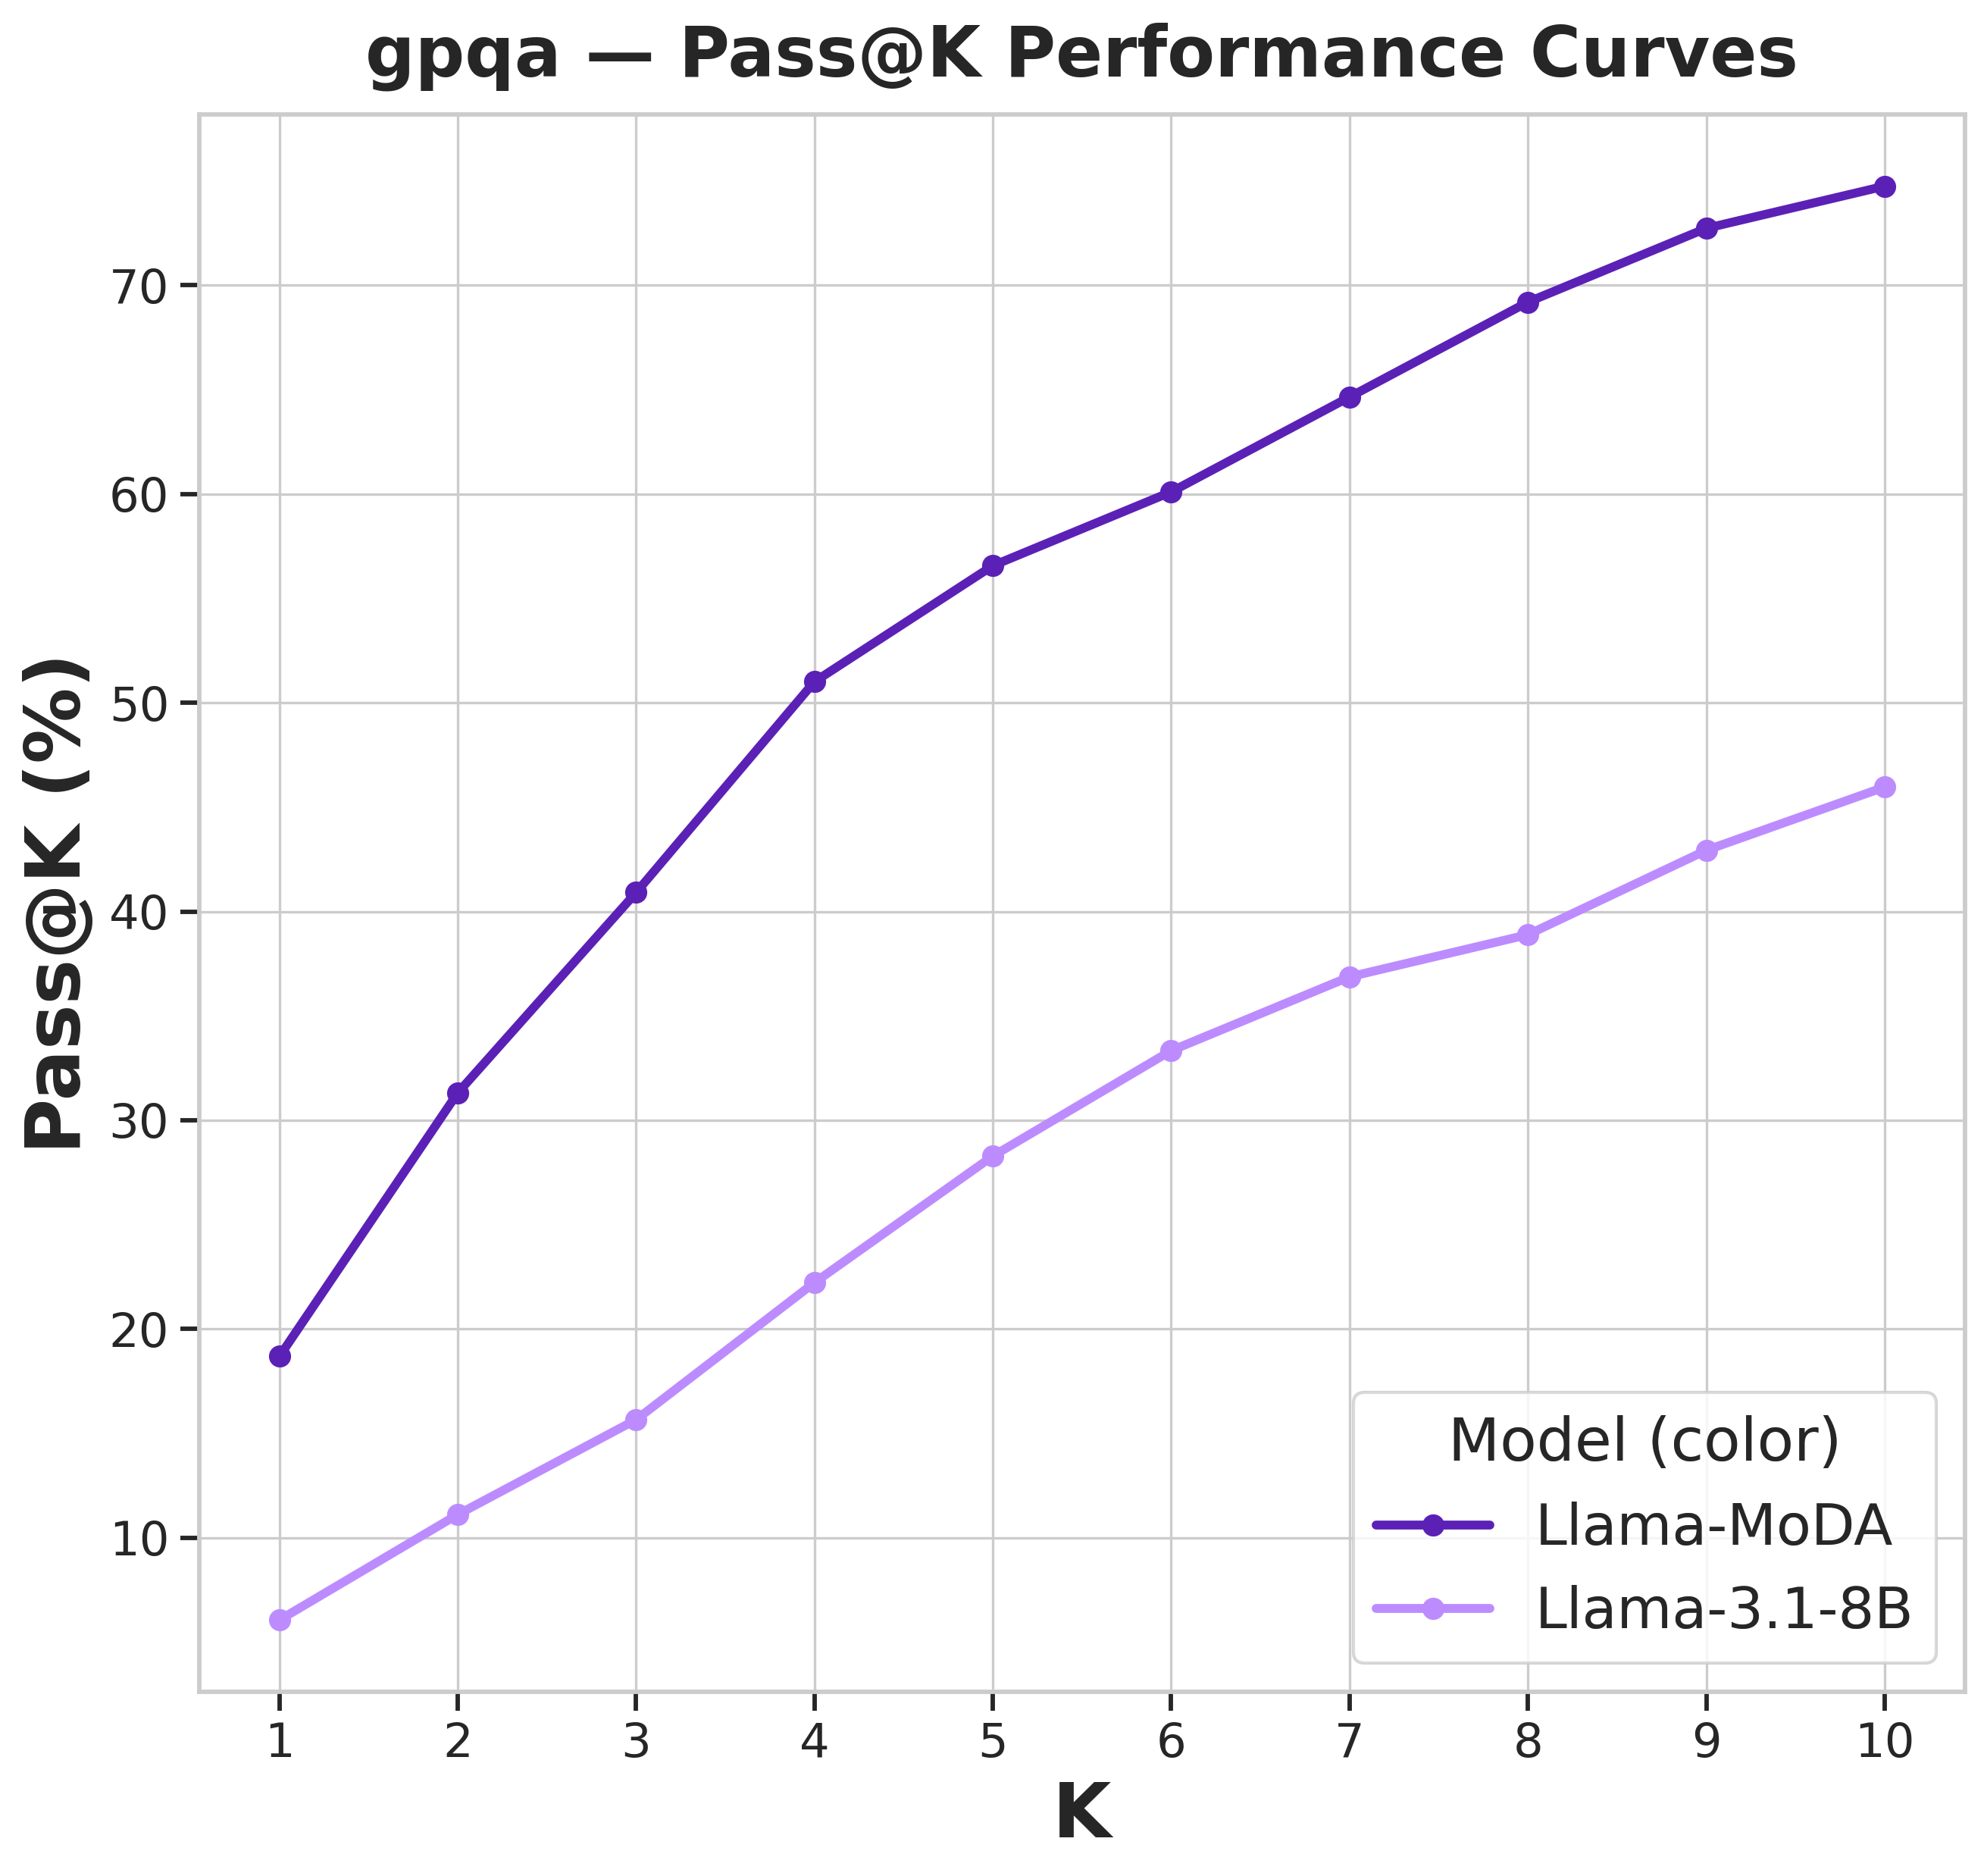
\includegraphics[width=\linewidth]{figures/main_pass_k/pass_at_k_figures/pass_at_k_gpqa_thinking_false_base_model_llama3_1-8b.png}
\end{minipage}\hfill
\begin{minipage}{0.24\textwidth}
  \centering
  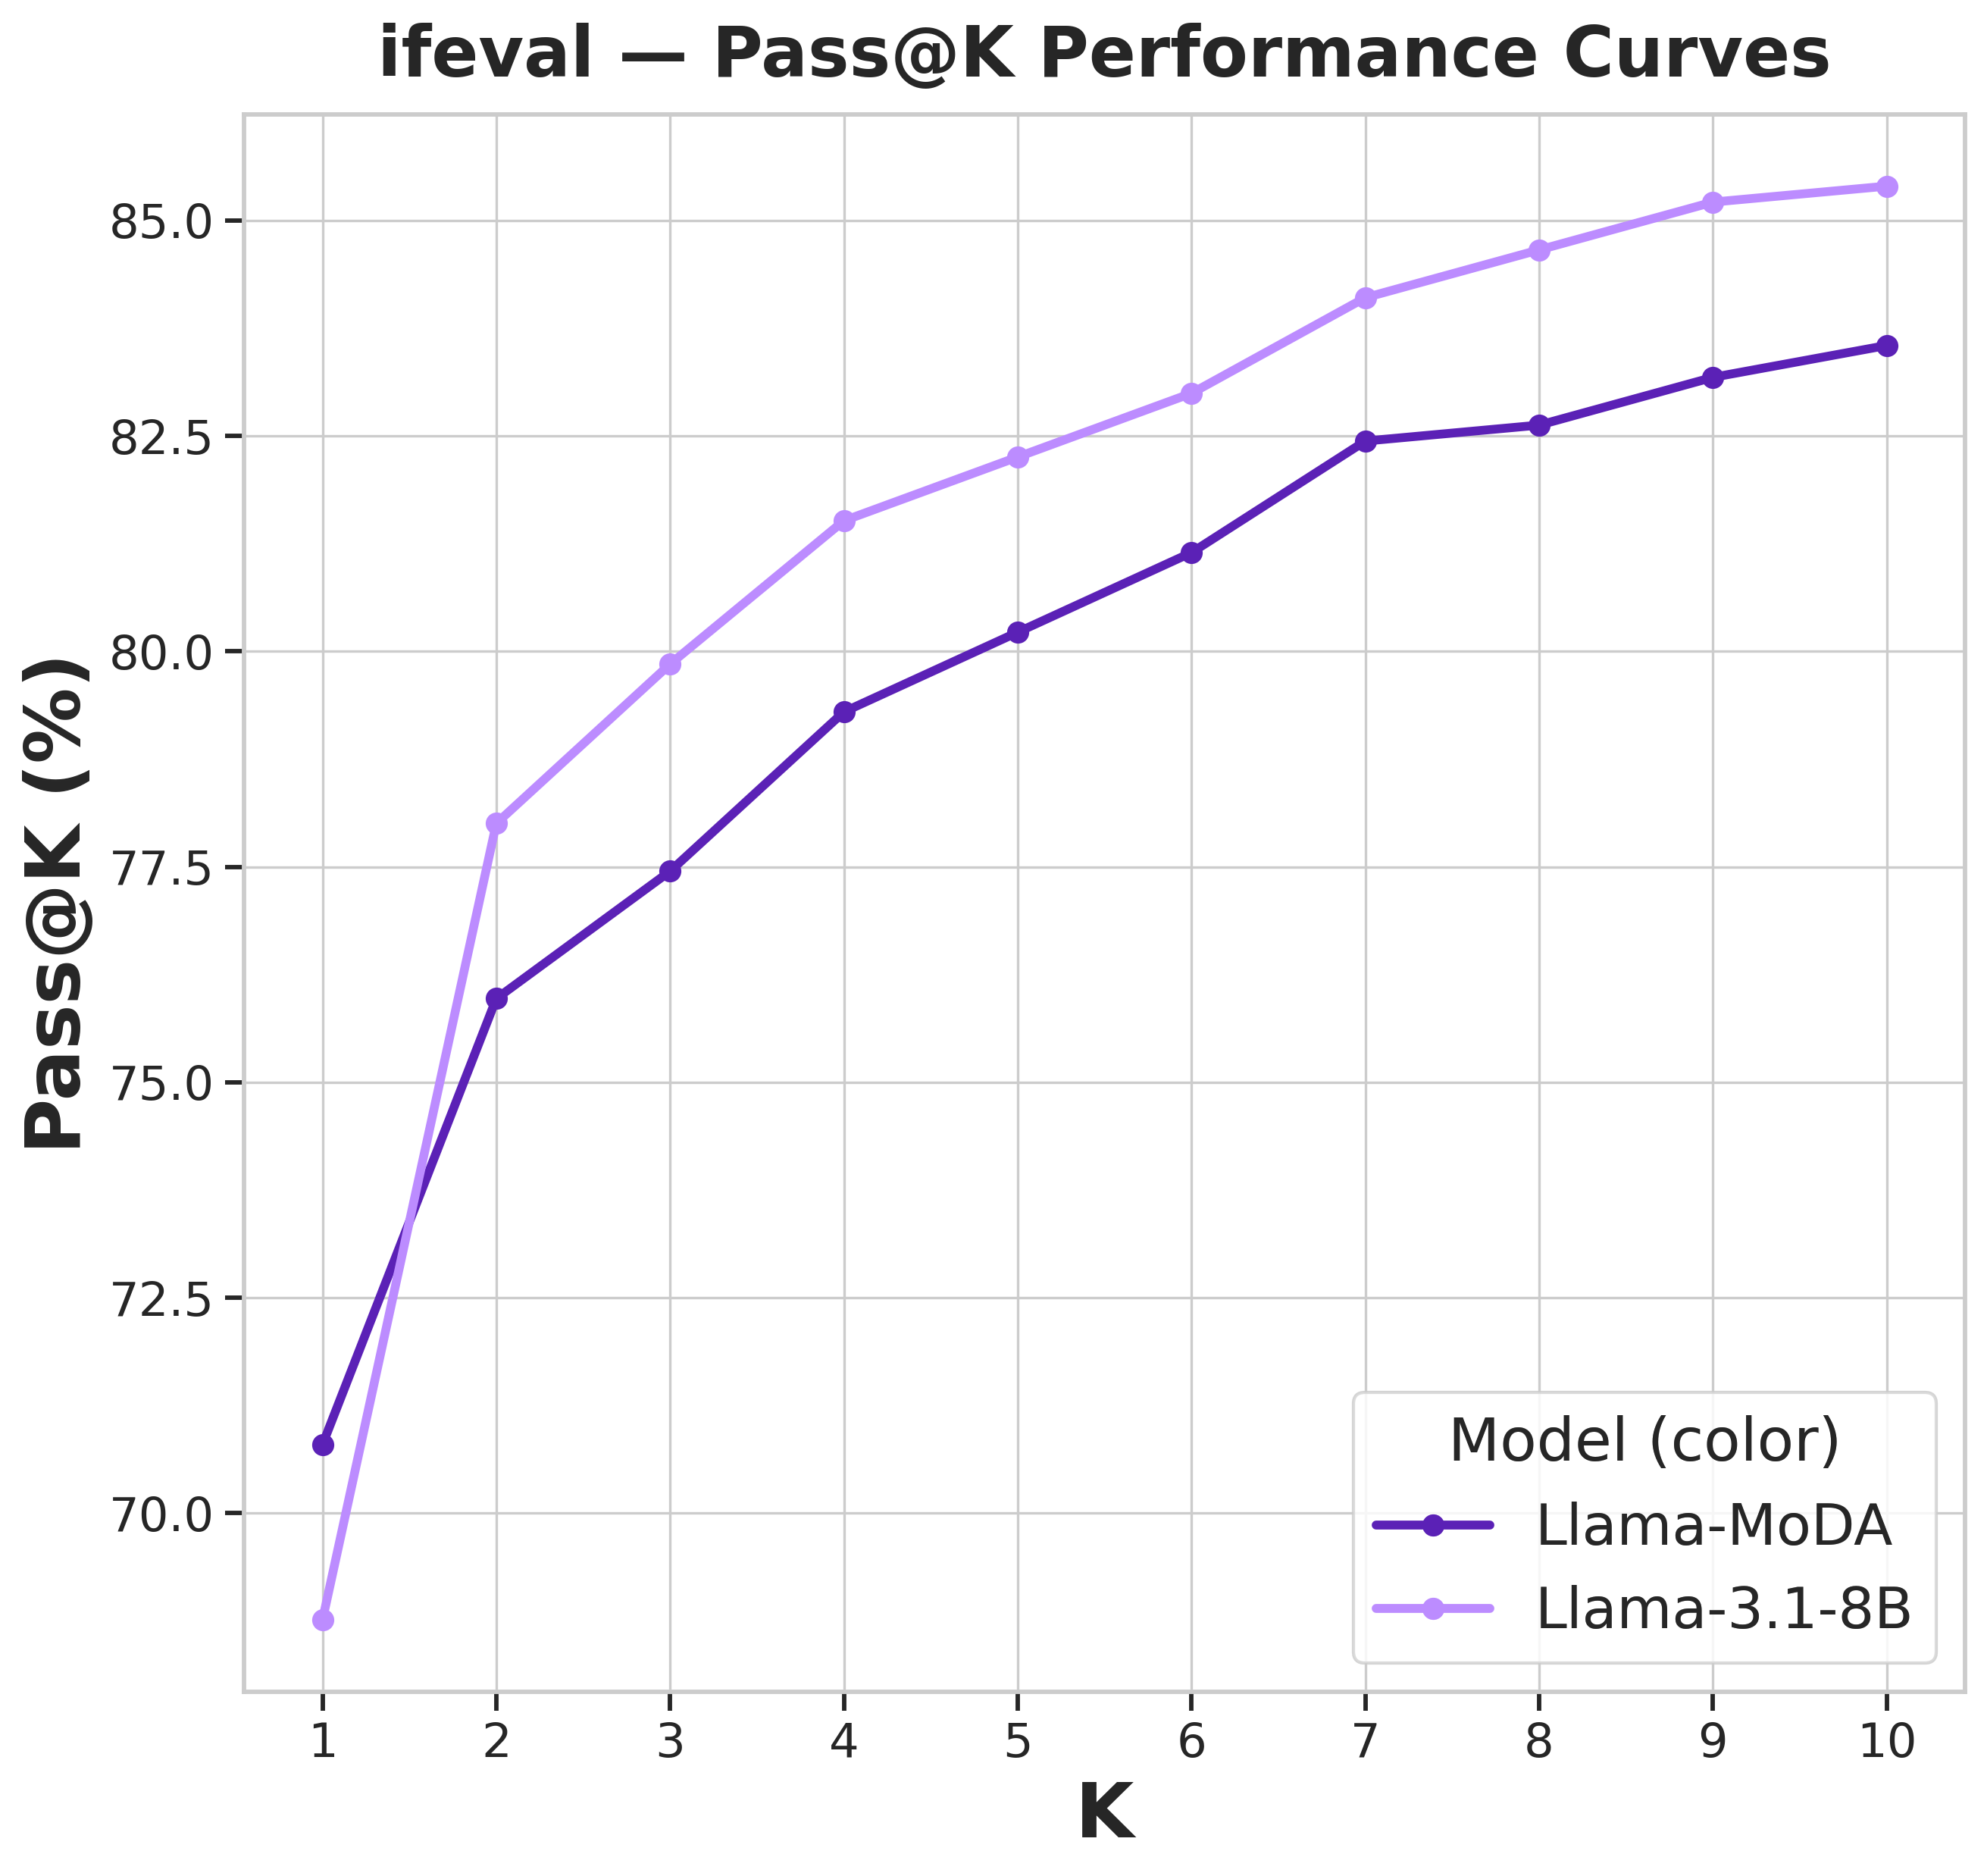
\includegraphics[width=\linewidth]{figures/main_pass_k/pass_at_k_figures/pass_at_k_ifeval_thinking_false_base_model_llama3_1-8b.png}
\end{minipage}
\caption{\textbf{General capability retention: pass@k accuracy.} Llama-3.1-8B base and thinking disabled models.}
\label{fig:general capability pass@k llama}
\end{figure}



\begin{figure}[H]
\begin{minipage}{0.24\textwidth}
  \centering
  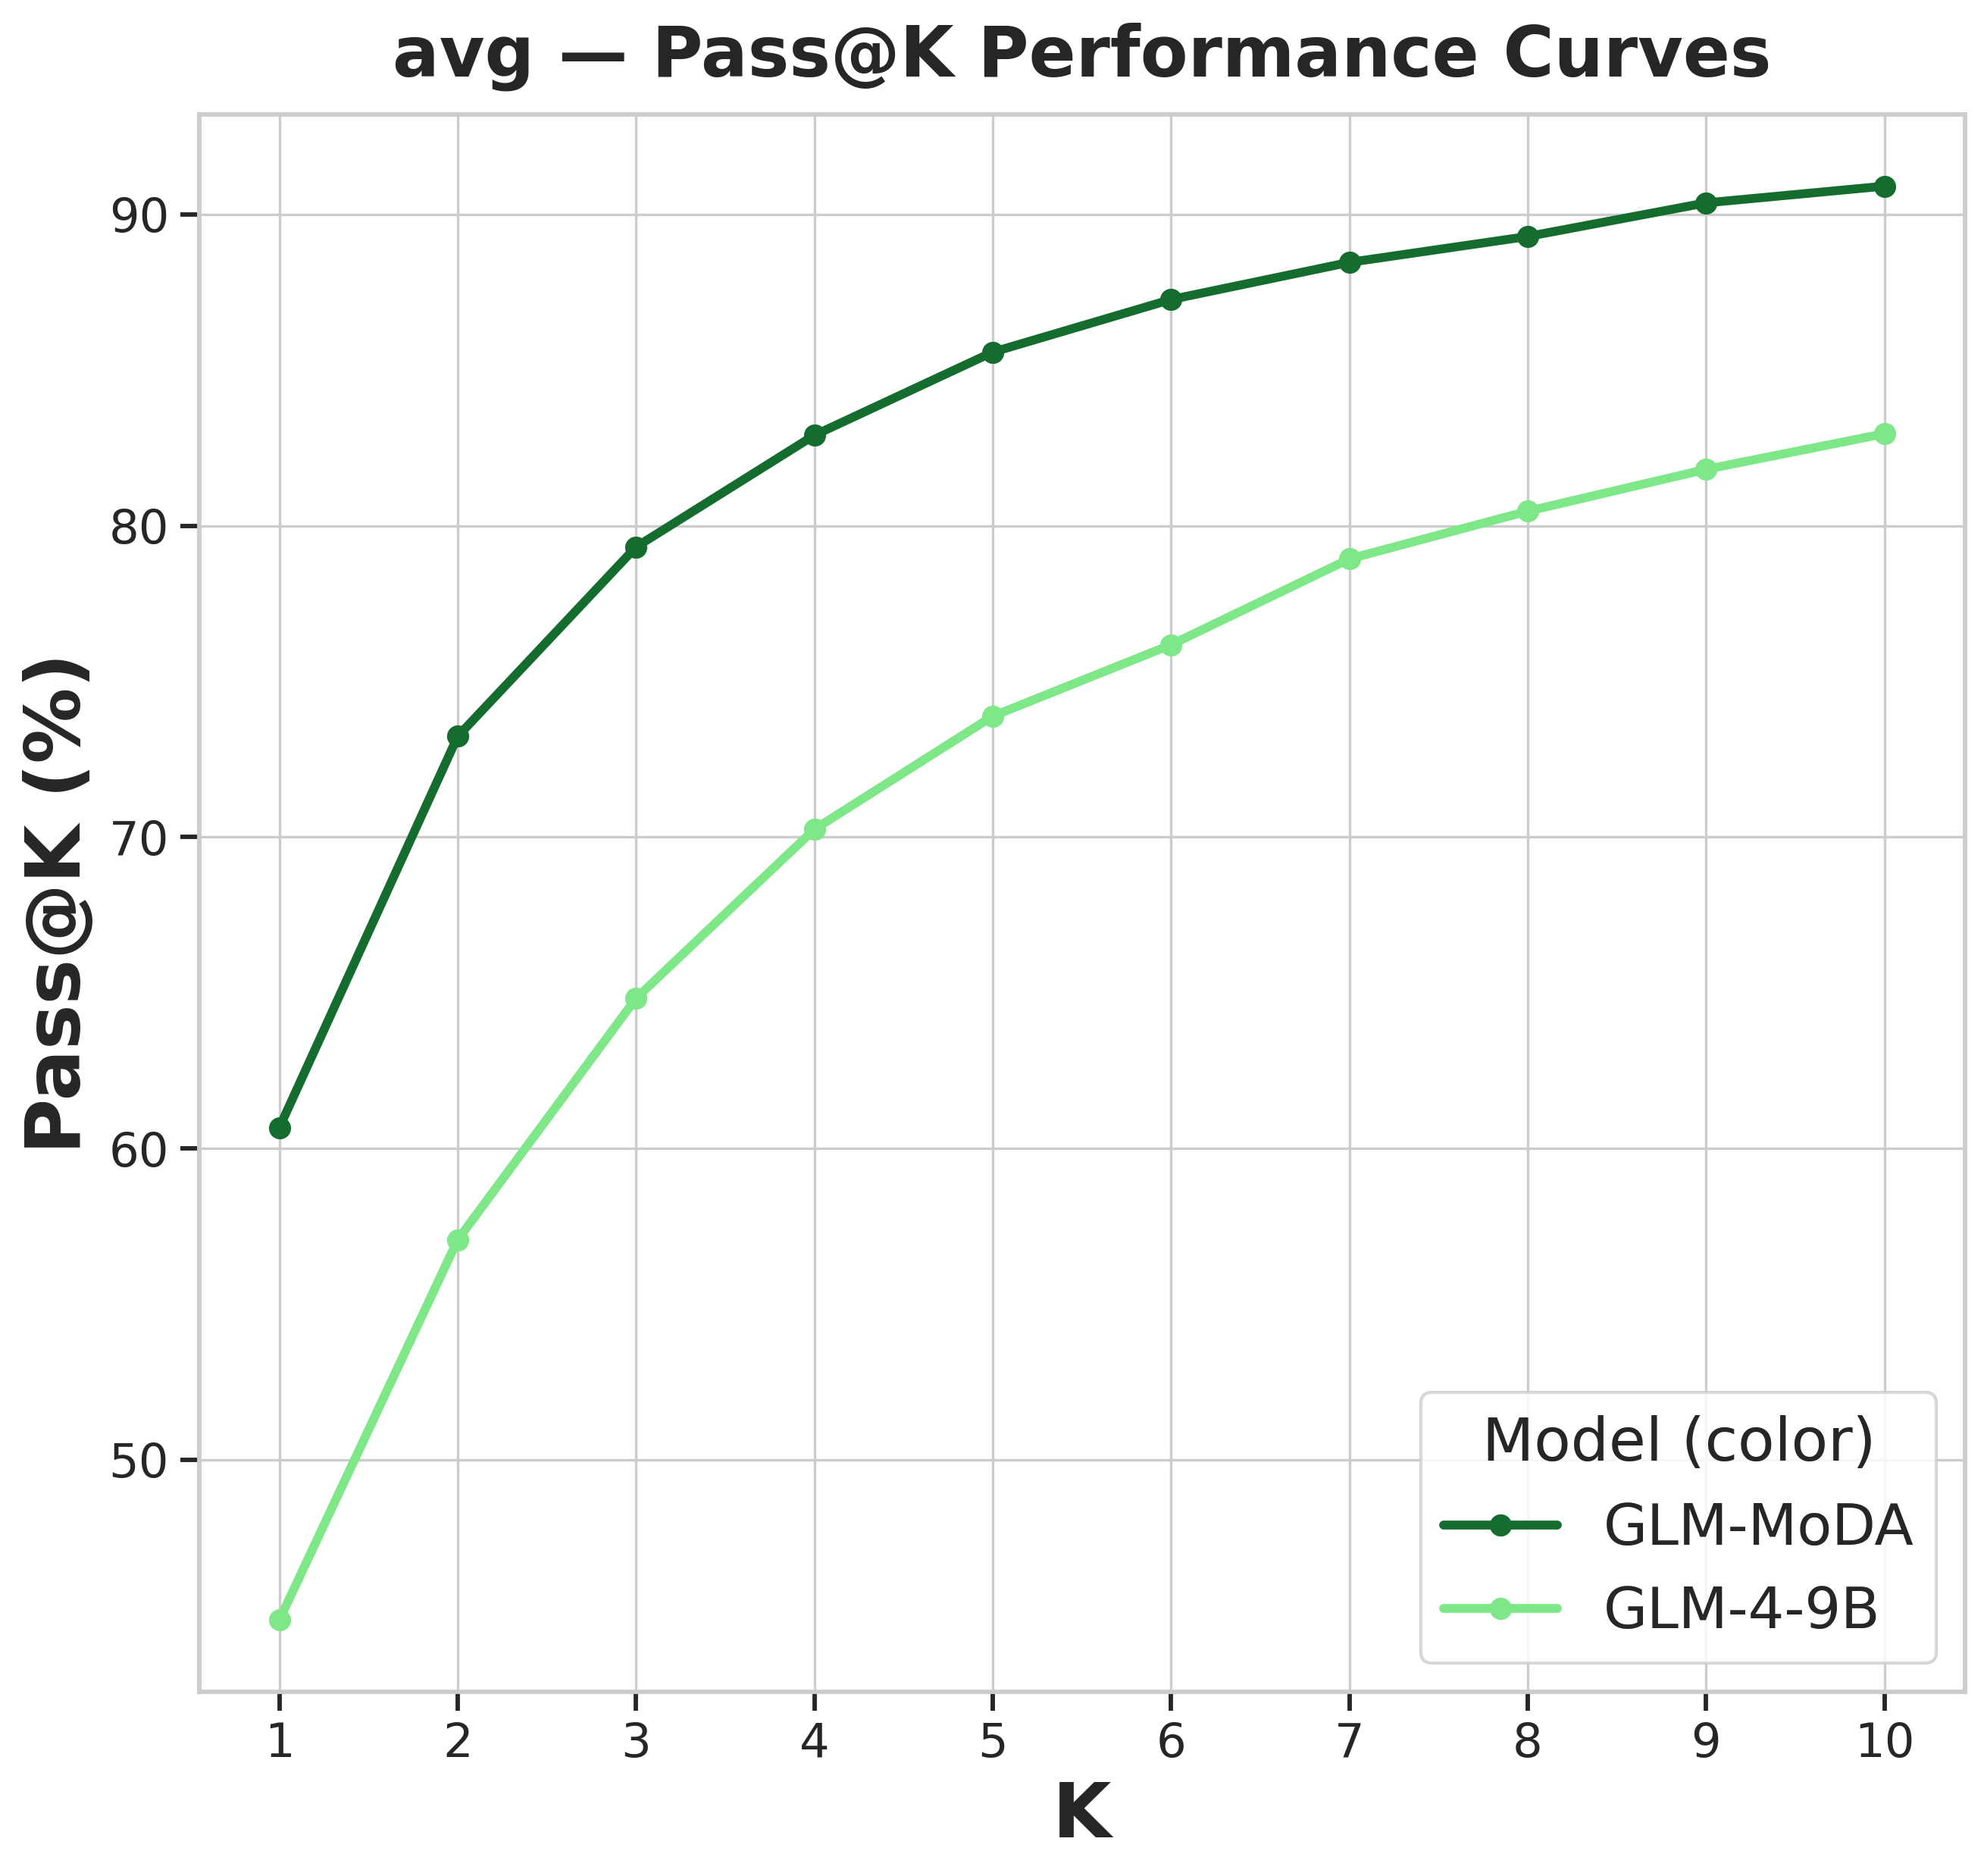
\includegraphics[width=\linewidth]{figures/main_pass_k/pass_at_k_figures/pass_at_k_avg_thinking_false_base_model_glm-4-9b.png}
\end{minipage}\hfill
\centering
\begin{minipage}{0.24\textwidth}
  \centering
  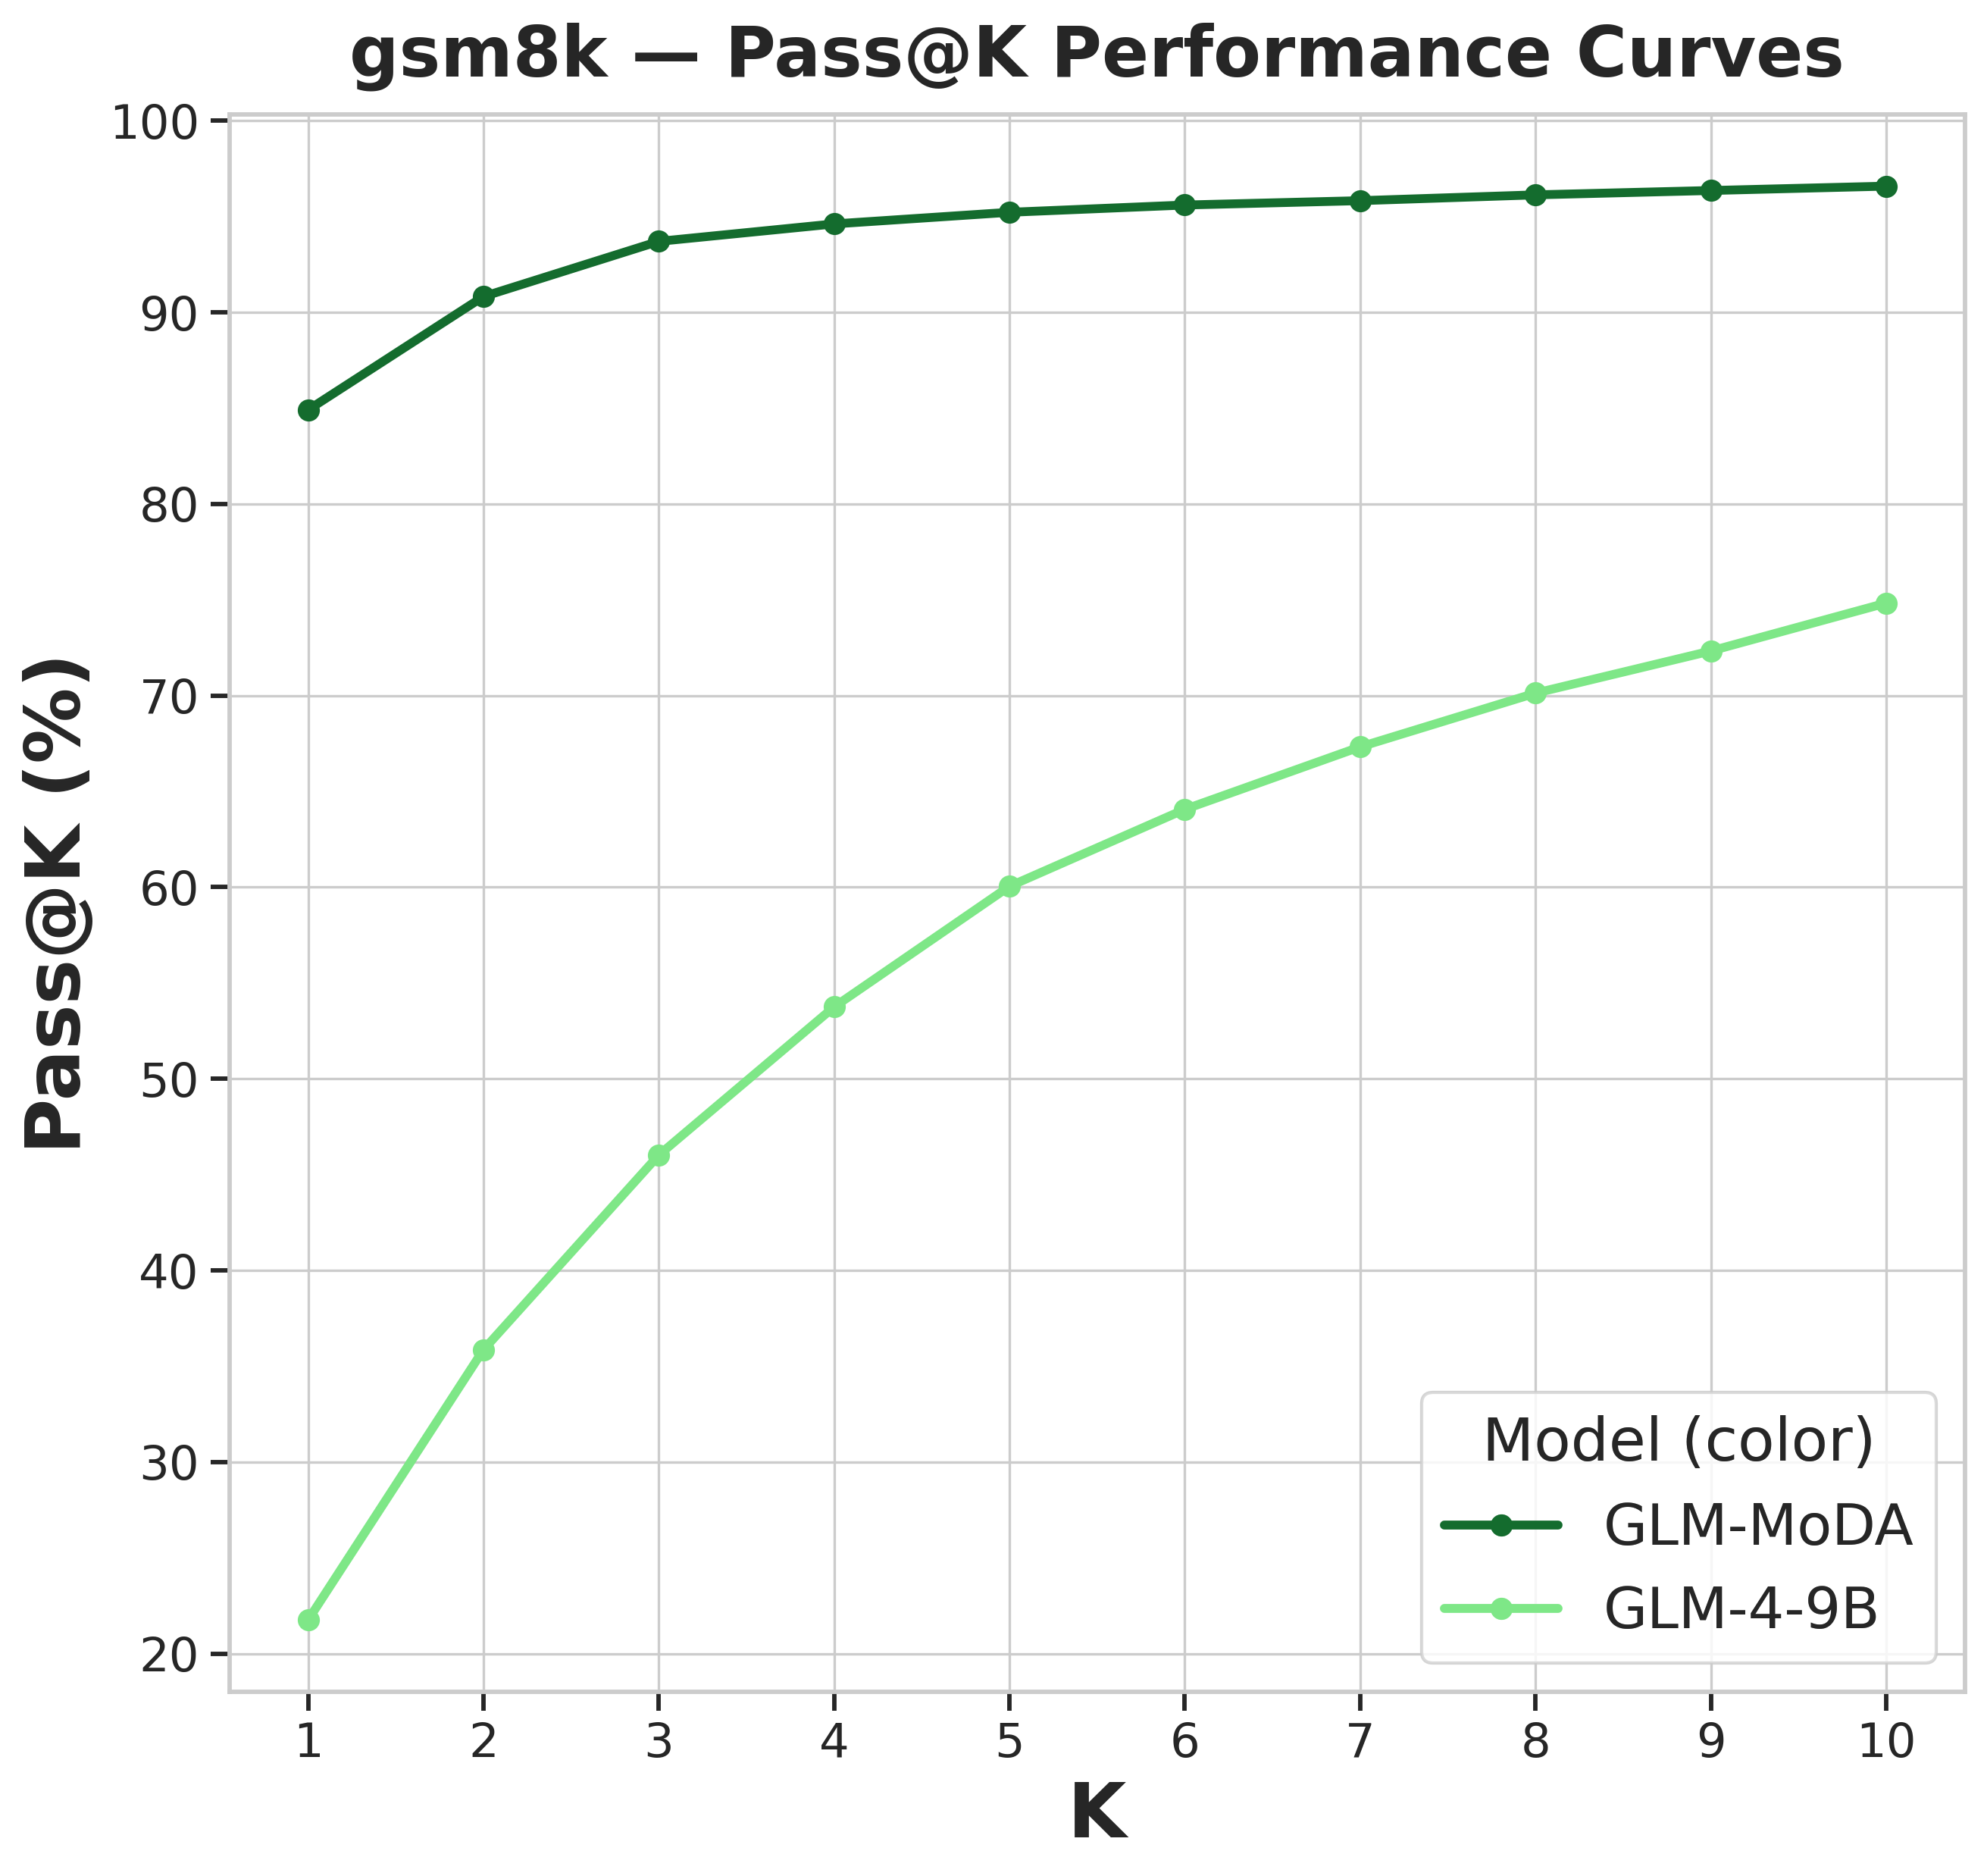
\includegraphics[width=\linewidth]{figures/main_pass_k/pass_at_k_figures/pass_at_k_gsm8k_thinking_false_base_model_glm-4-9b.png}
\end{minipage}\hfill
\begin{minipage}{0.24\textwidth}
  \centering
  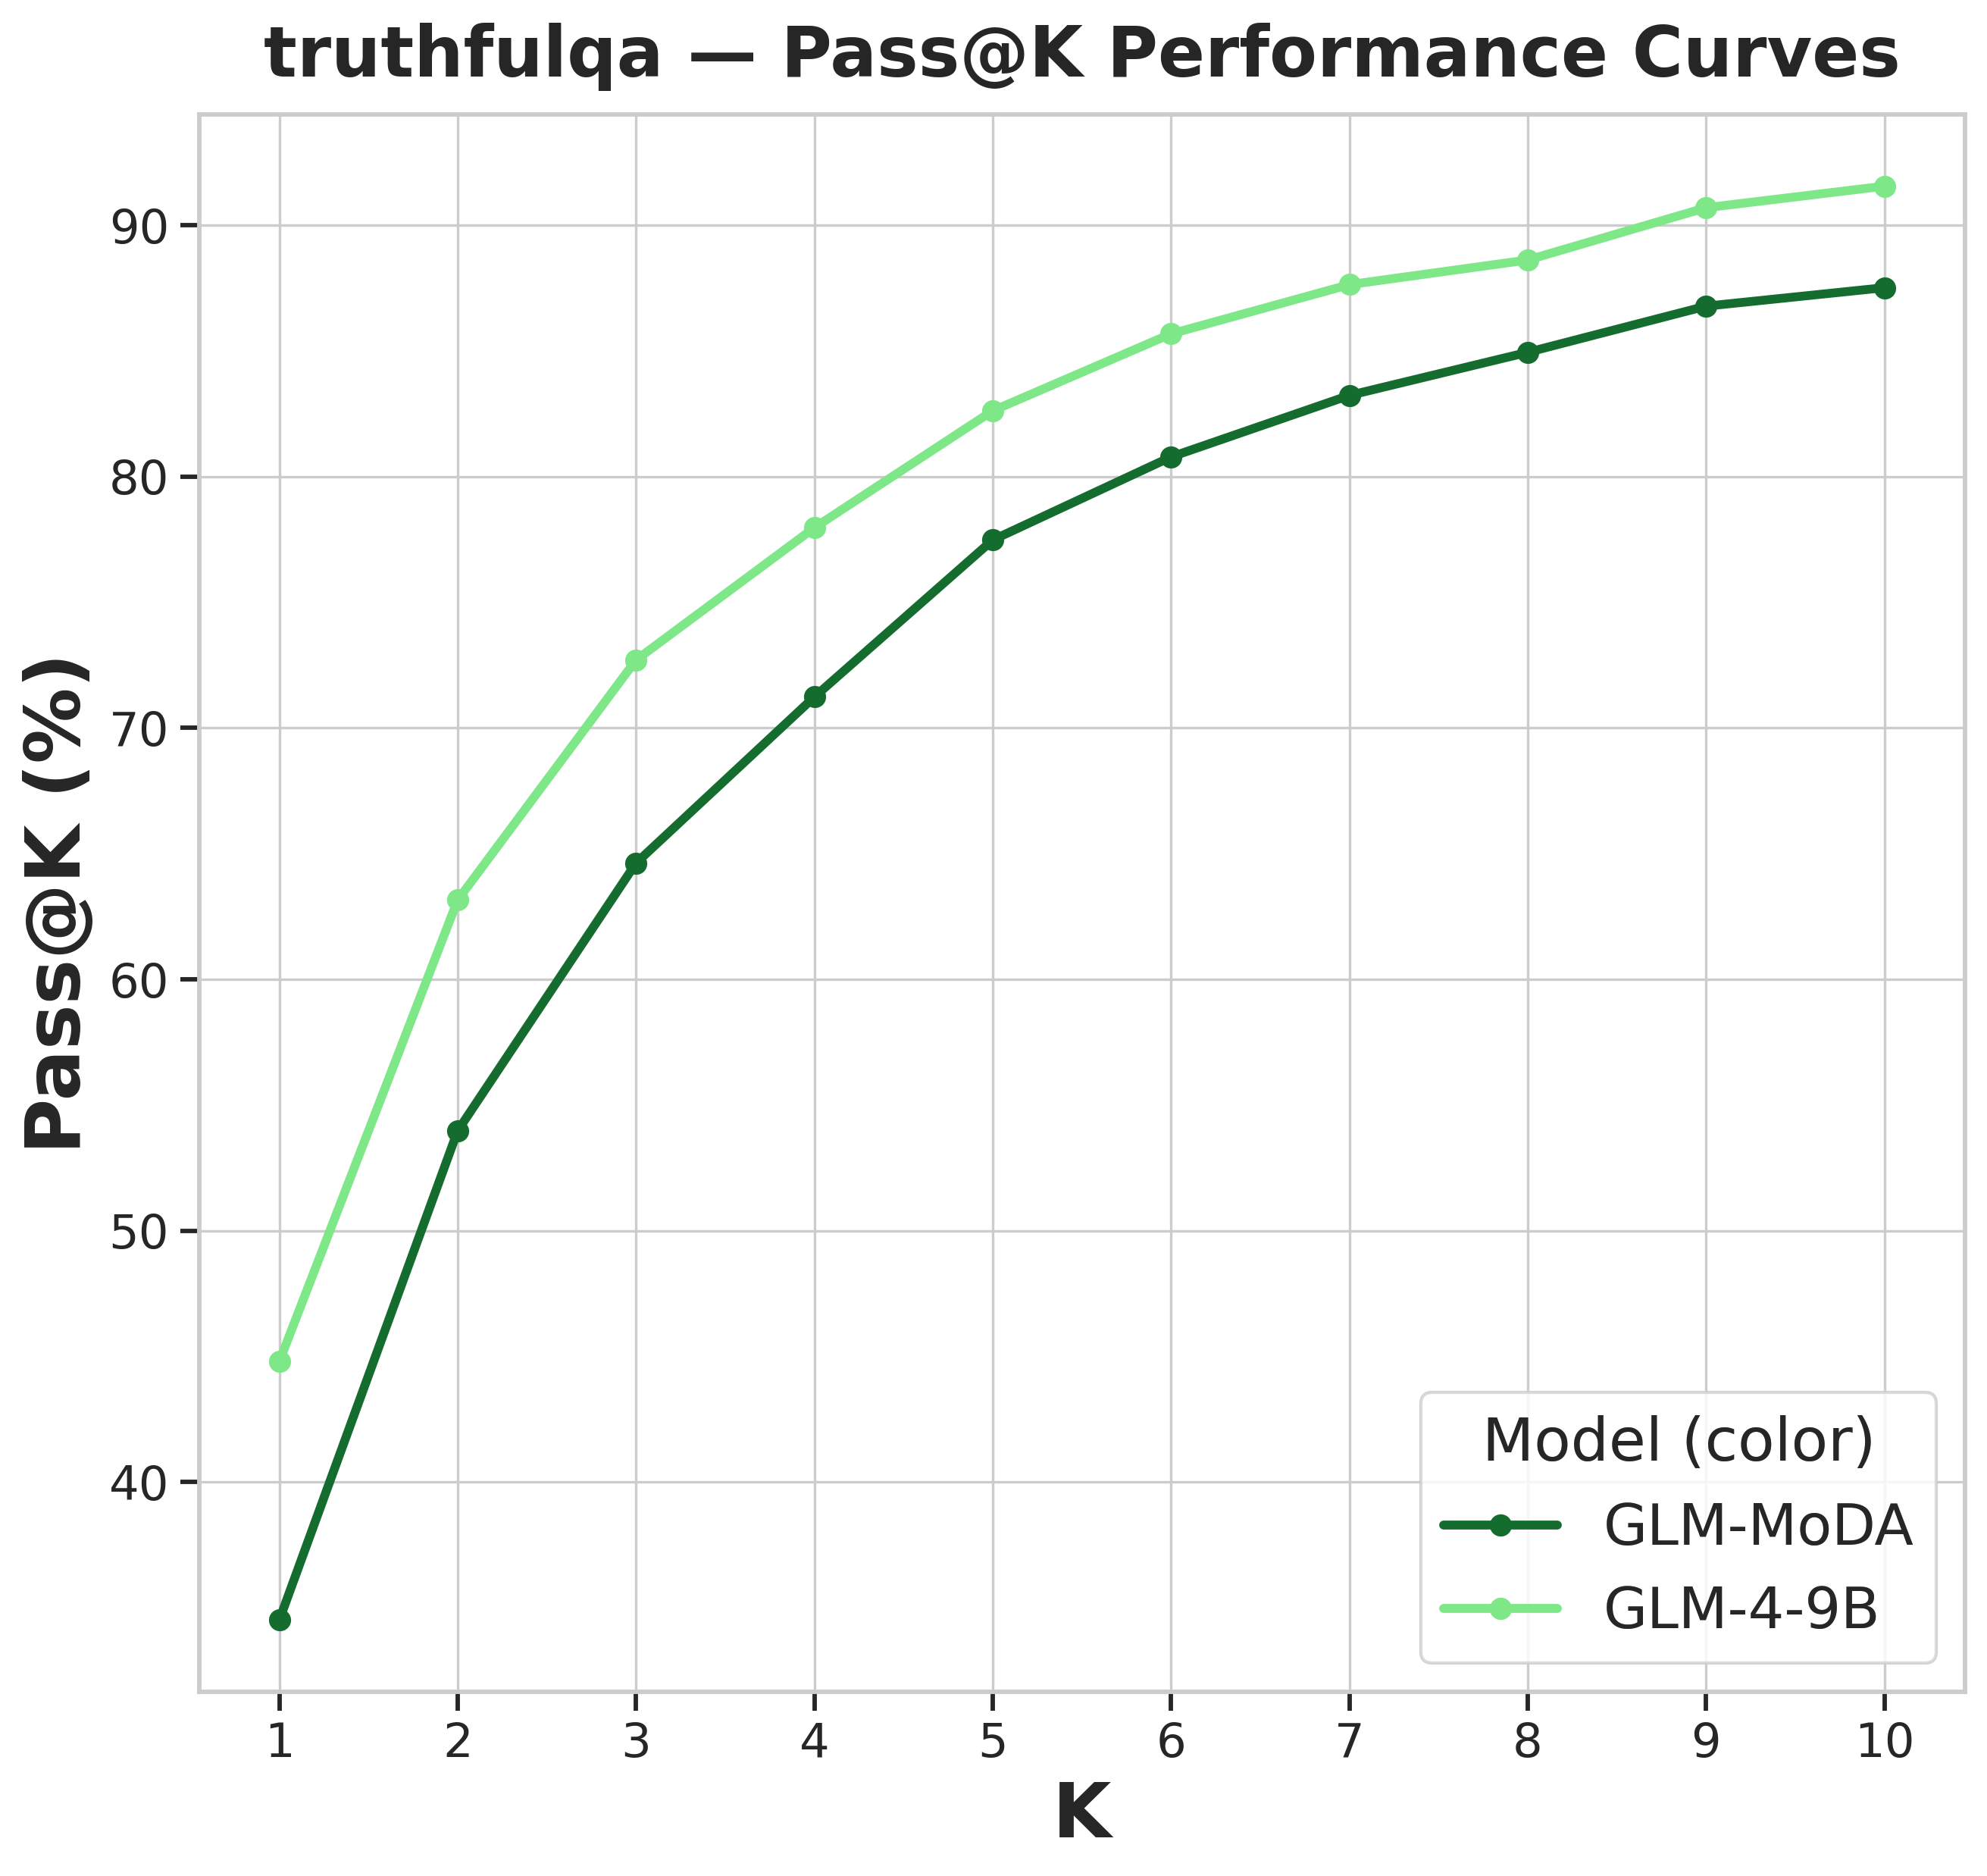
\includegraphics[width=\linewidth]{figures/main_pass_k/pass_at_k_figures/pass_at_k_truthfulqa_thinking_false_base_model_glm-4-9b.png}
\end{minipage}\hfill
\begin{minipage}{0.24\textwidth}
  \centering
  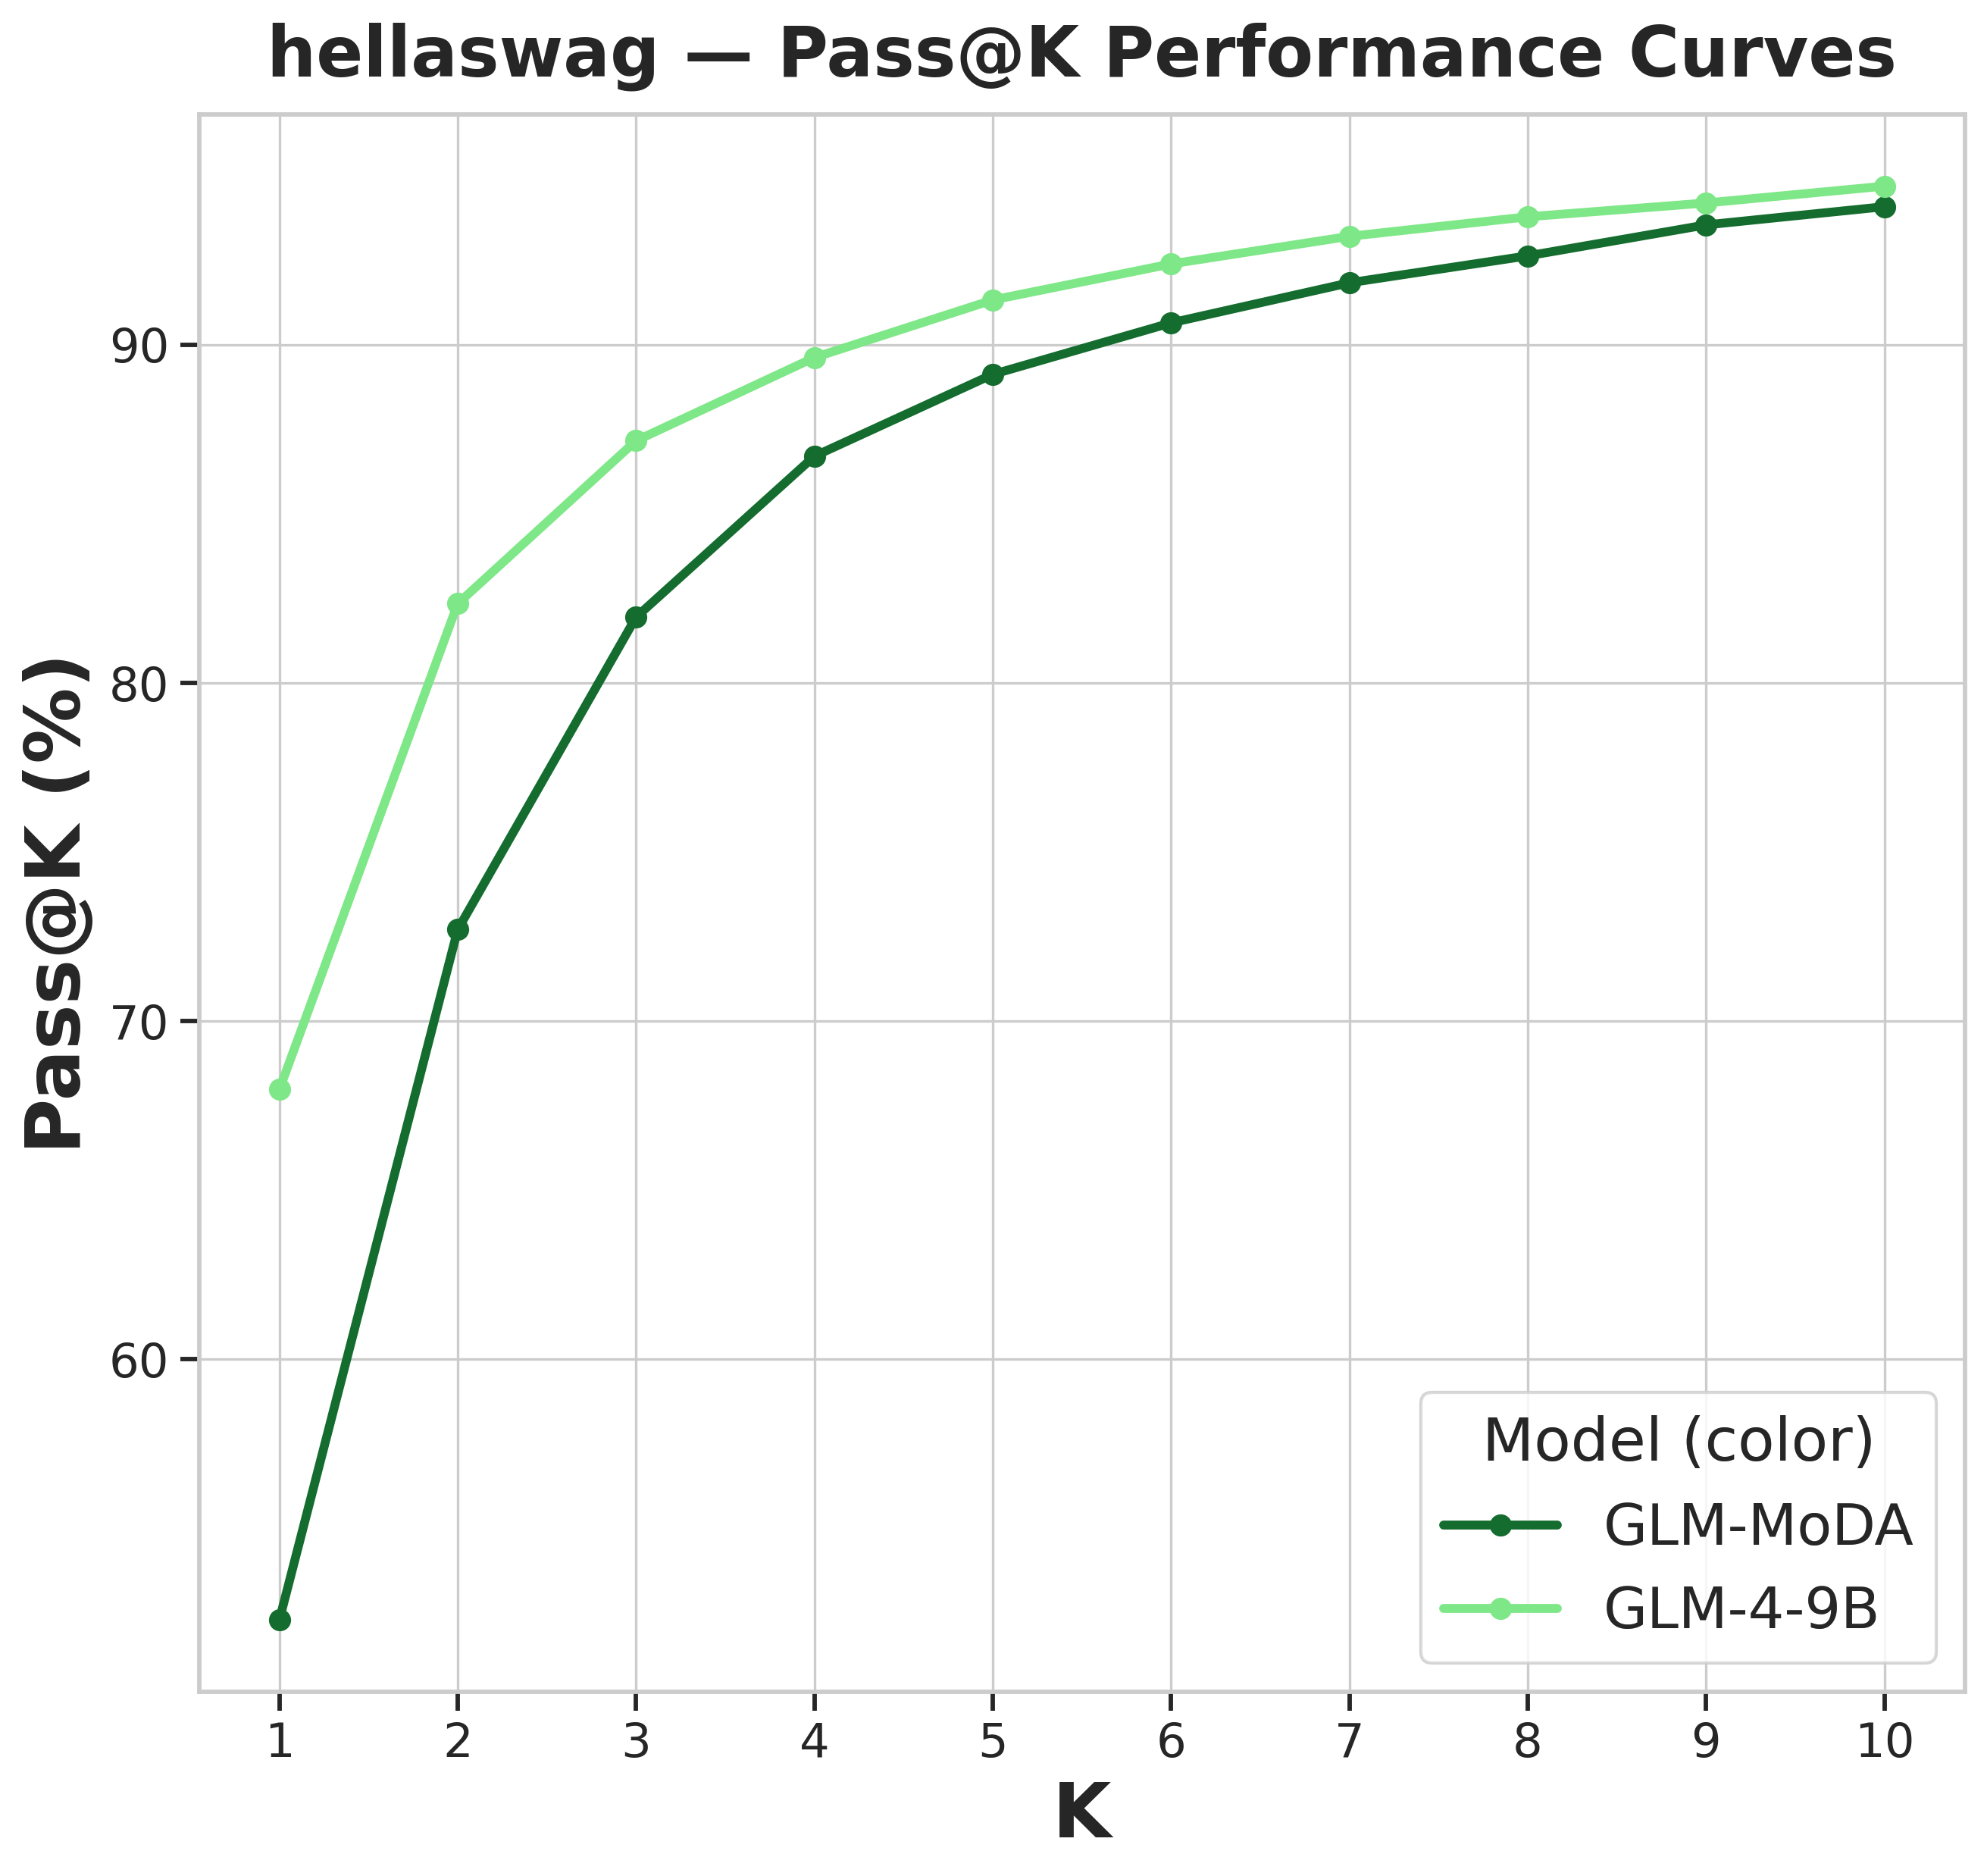
\includegraphics[width=\linewidth]{figures/main_pass_k/pass_at_k_figures/pass_at_k_hellaswag_thinking_false_base_model_glm-4-9b.png}
\end{minipage}
\centering
\begin{minipage}{0.24\textwidth}
  \centering
  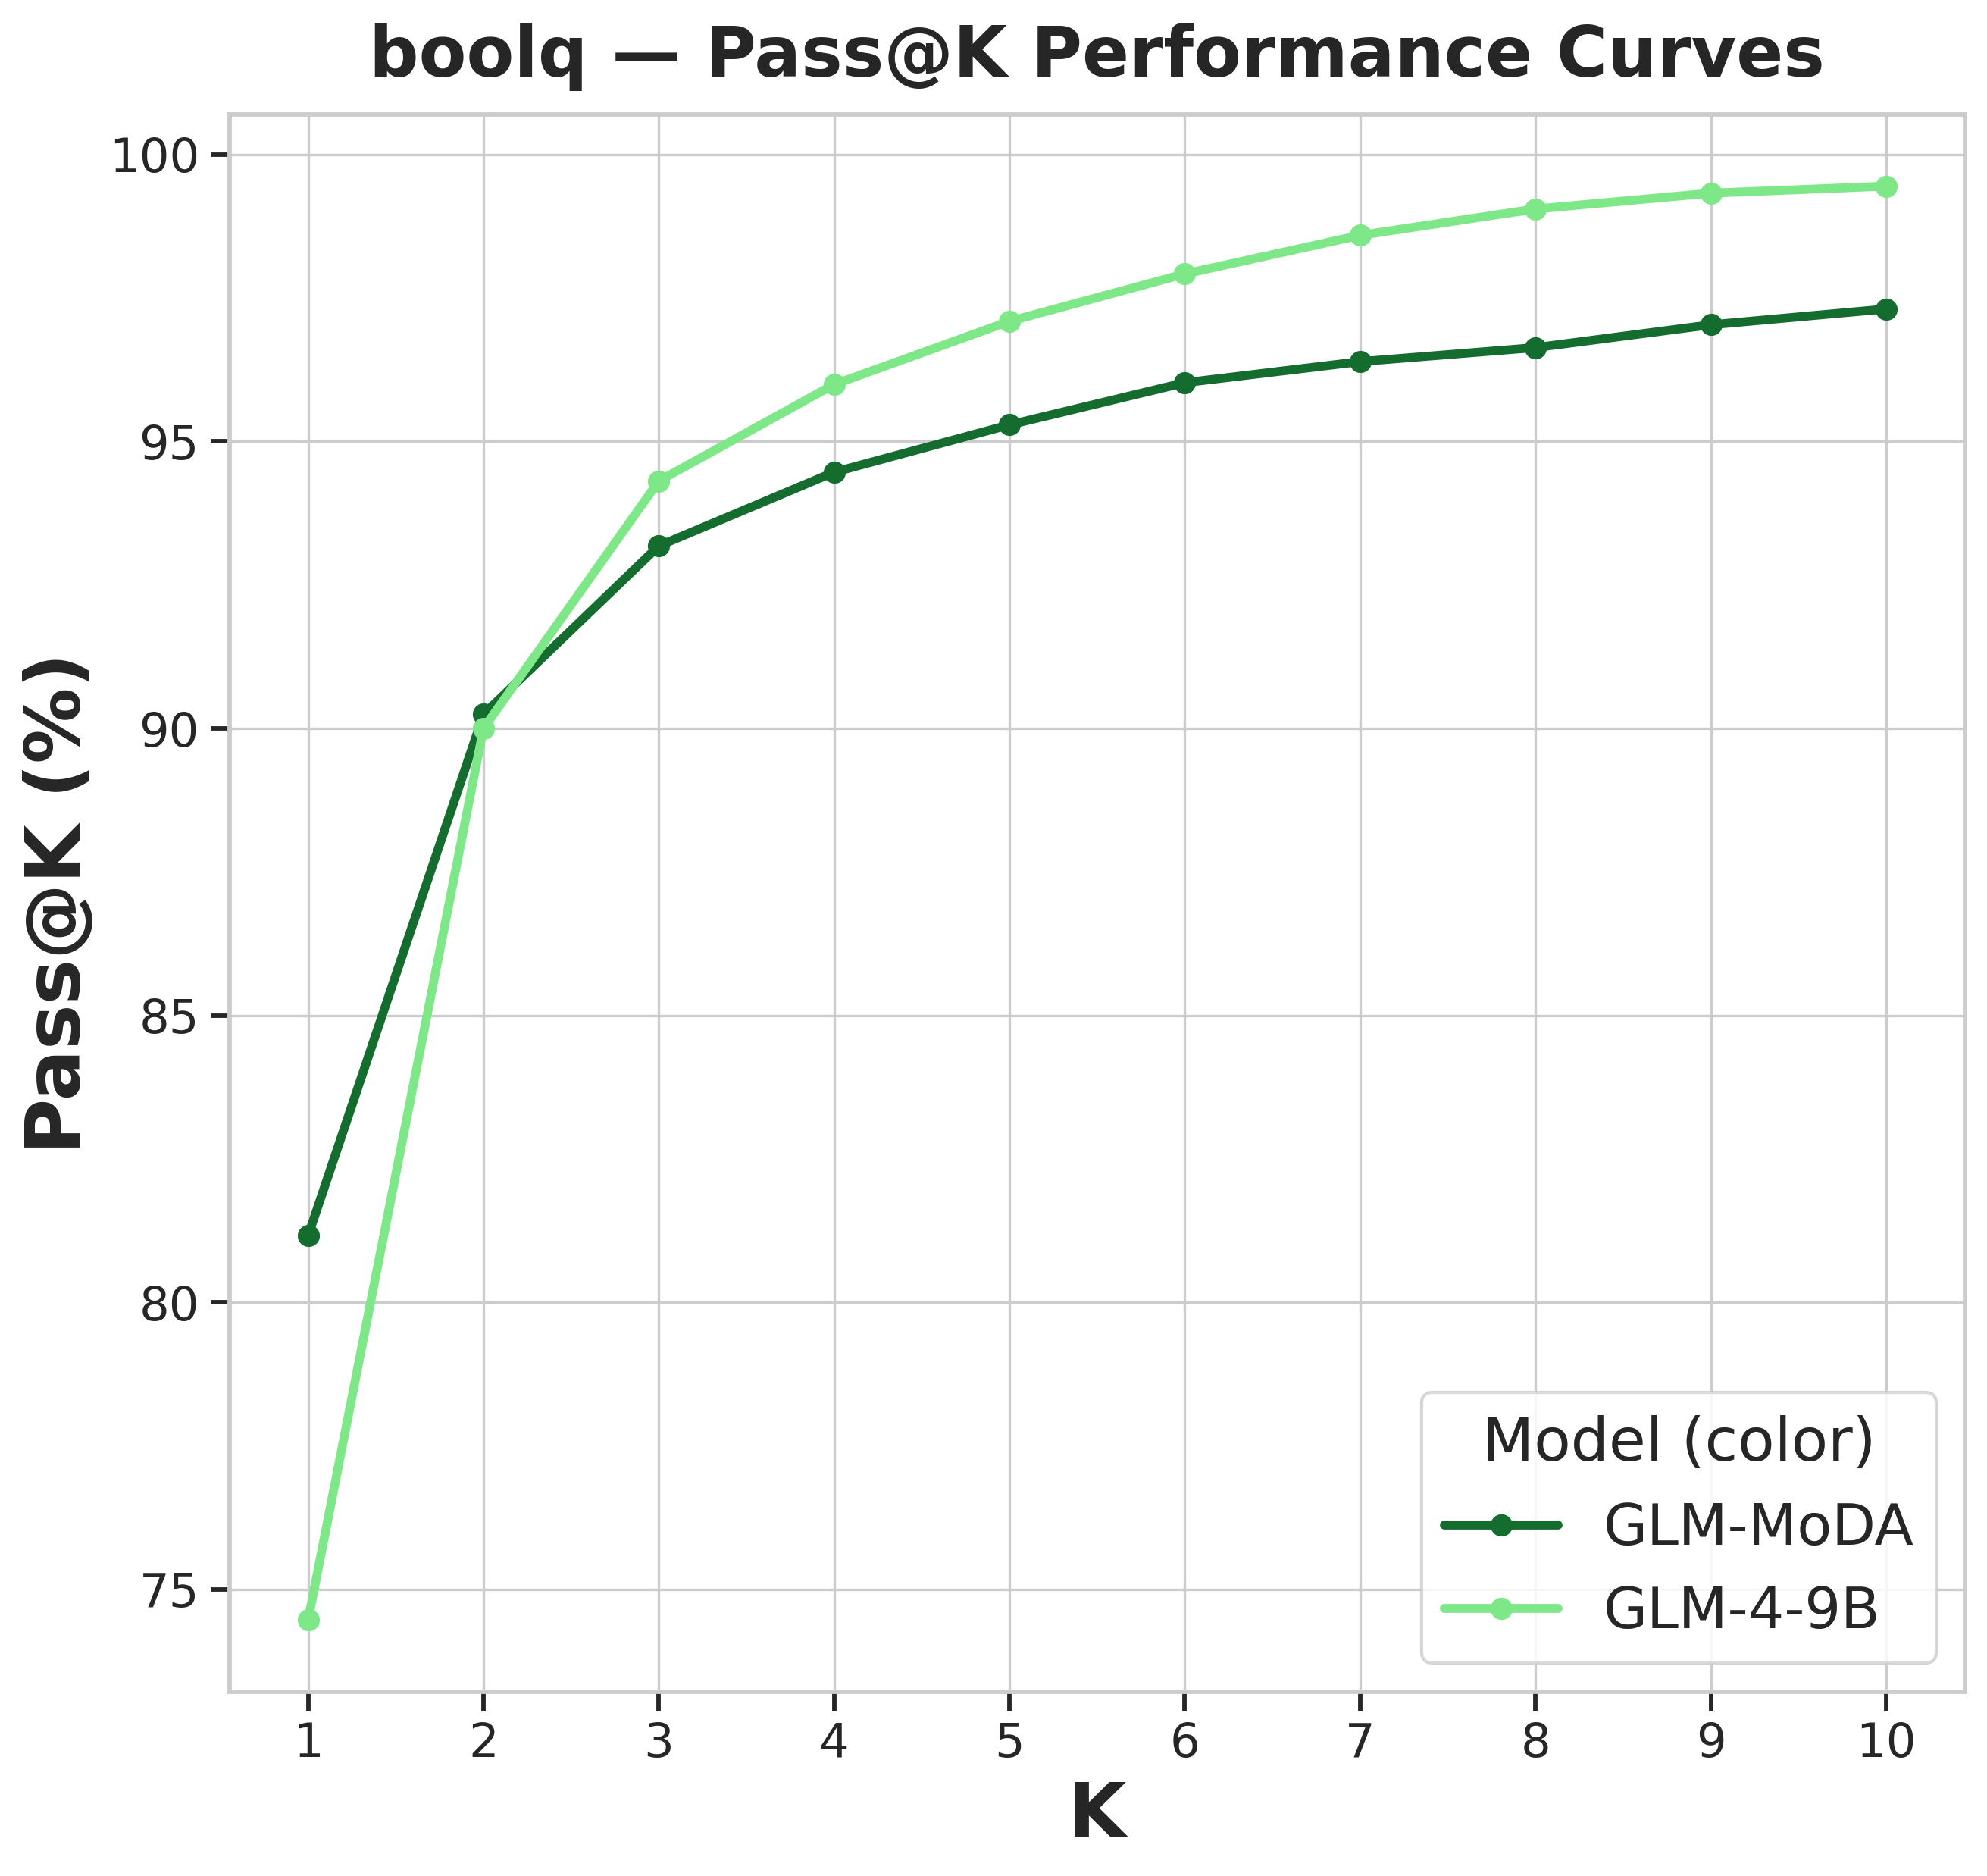
\includegraphics[width=\linewidth]{figures/main_pass_k/pass_at_k_figures/pass_at_k_boolq_thinking_false_base_model_glm-4-9b.png}
\end{minipage}\hfill
\centering
\begin{minipage}{0.24\textwidth}
  \centering
  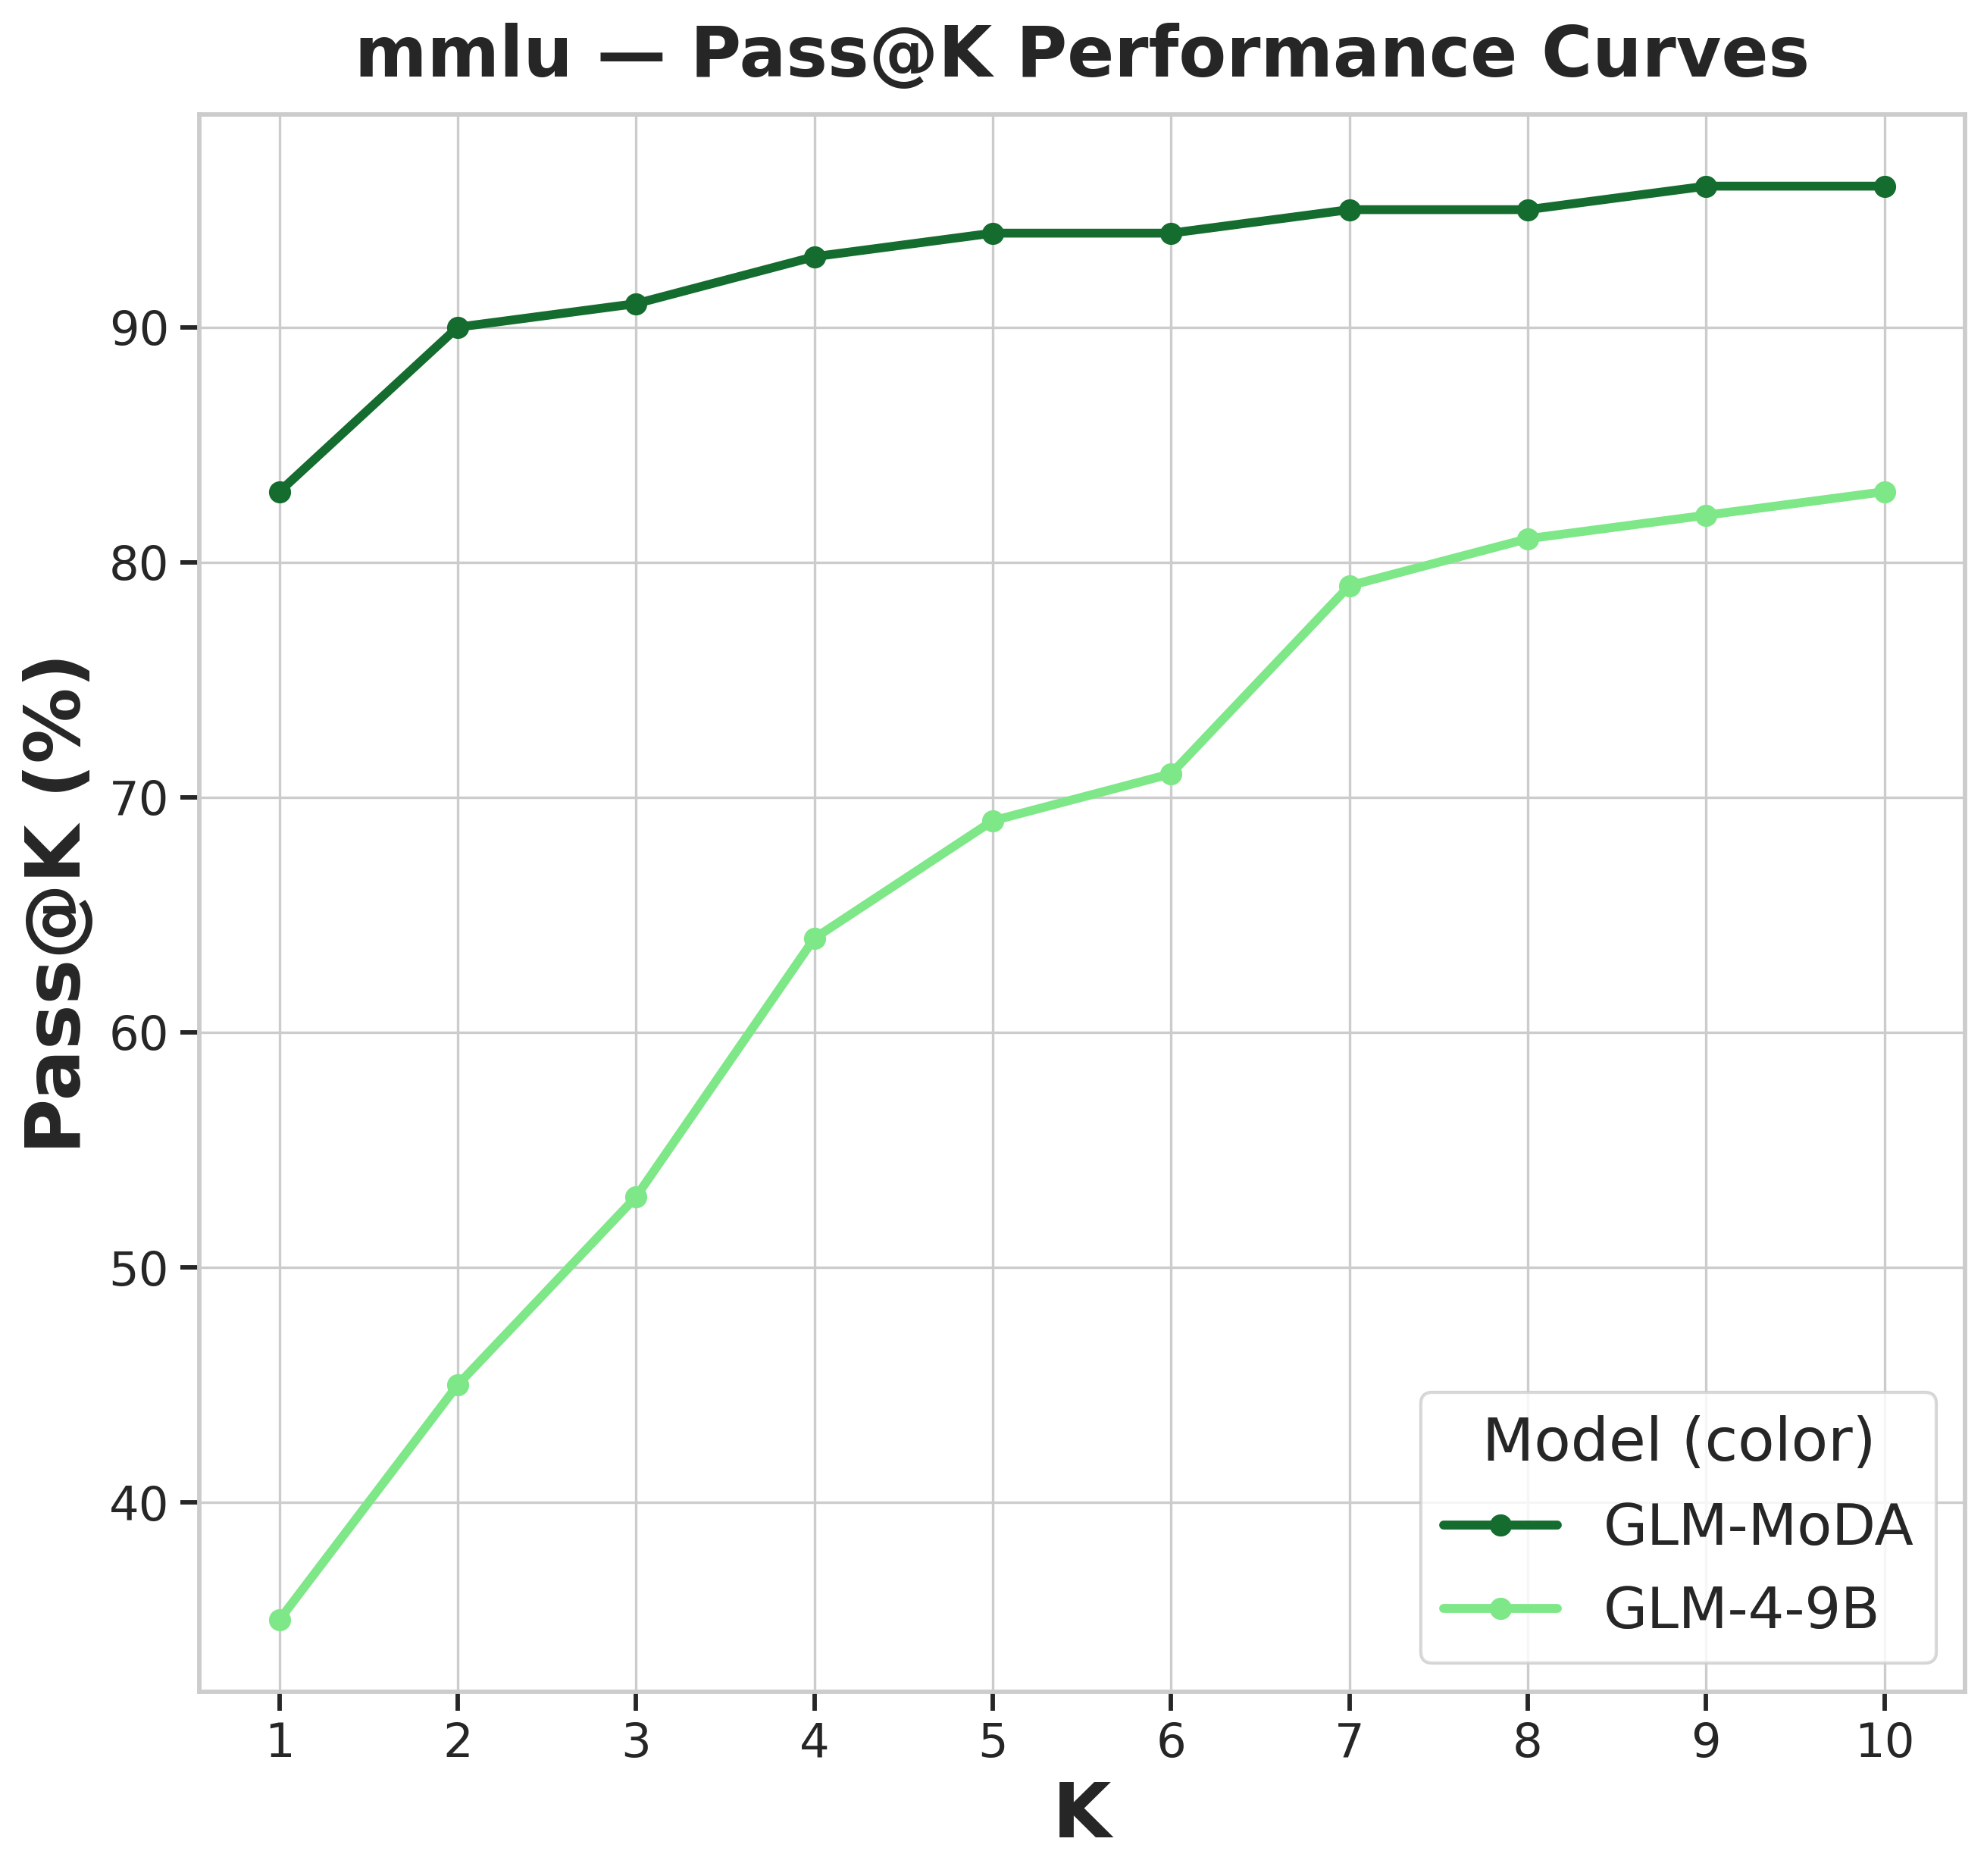
\includegraphics[width=\linewidth]{figures/main_pass_k/pass_at_k_figures/pass_at_k_mmlu_thinking_false_base_model_glm-4-9b.png}
\end{minipage}\hfill
\begin{minipage}{0.24\textwidth}
  \centering
  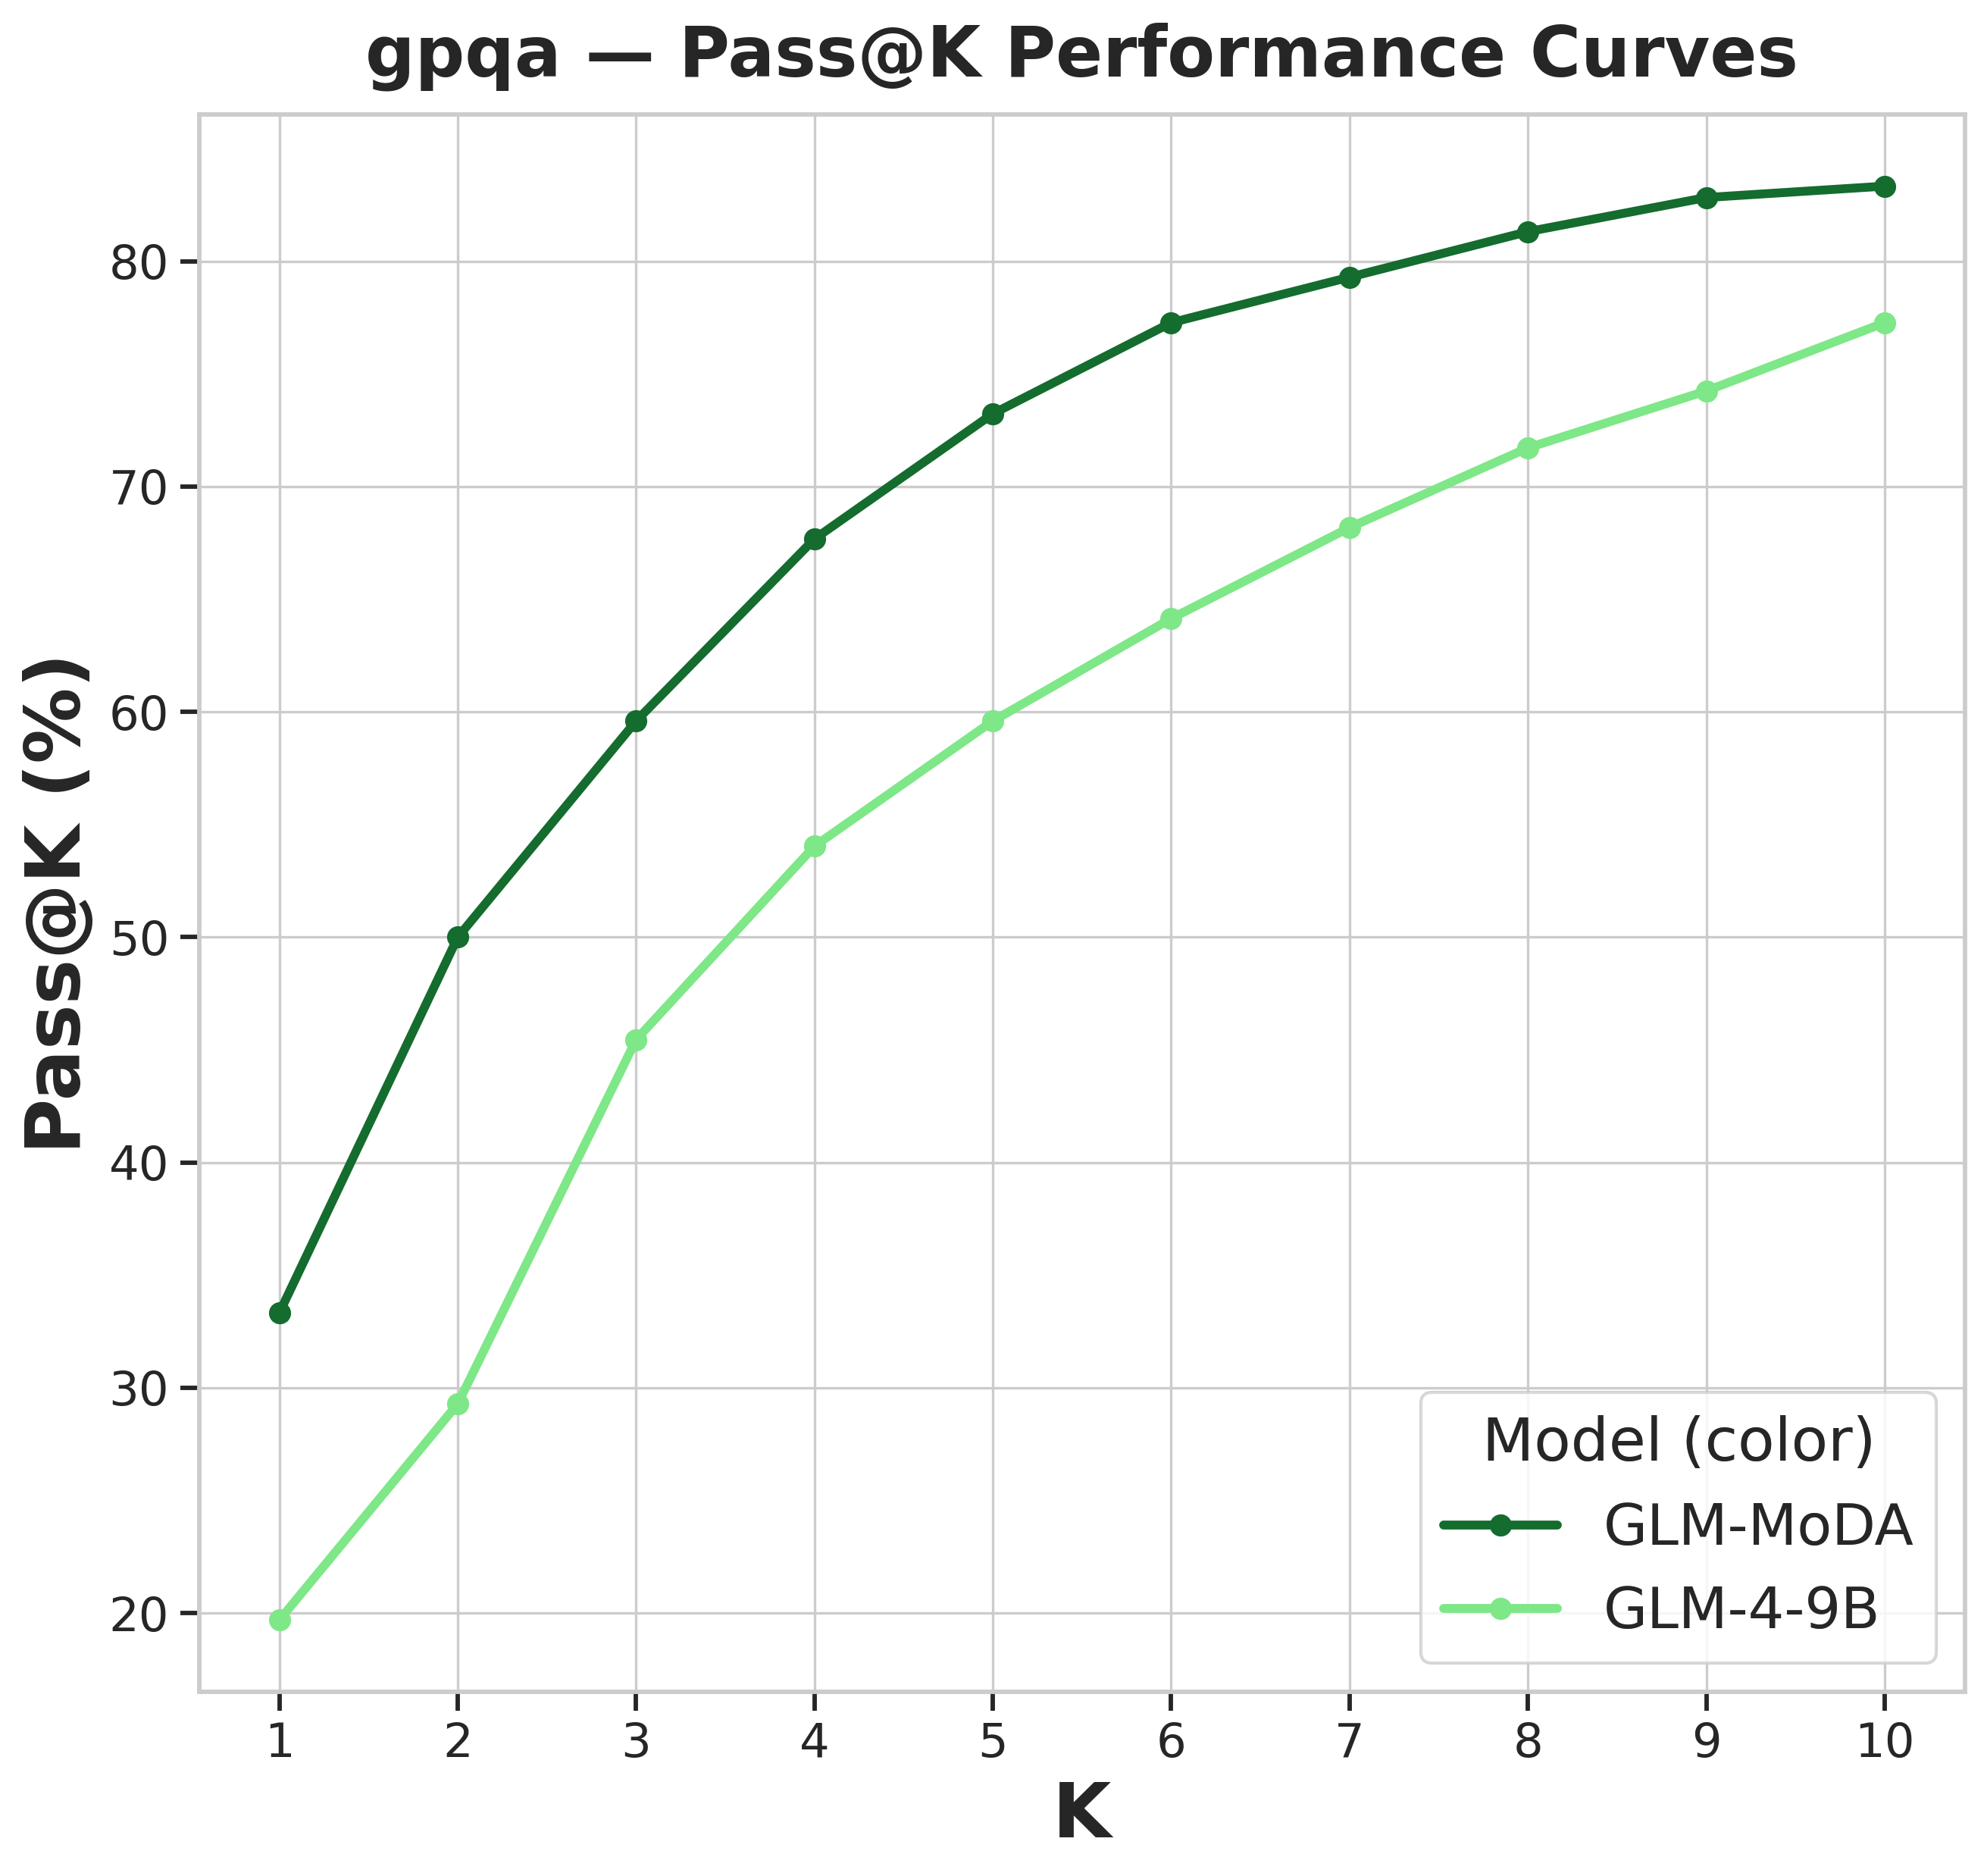
\includegraphics[width=\linewidth]{figures/main_pass_k/pass_at_k_figures/pass_at_k_gpqa_thinking_false_base_model_glm-4-9b.png}
\end{minipage}\hfill
\begin{minipage}{0.24\textwidth}
  \centering
  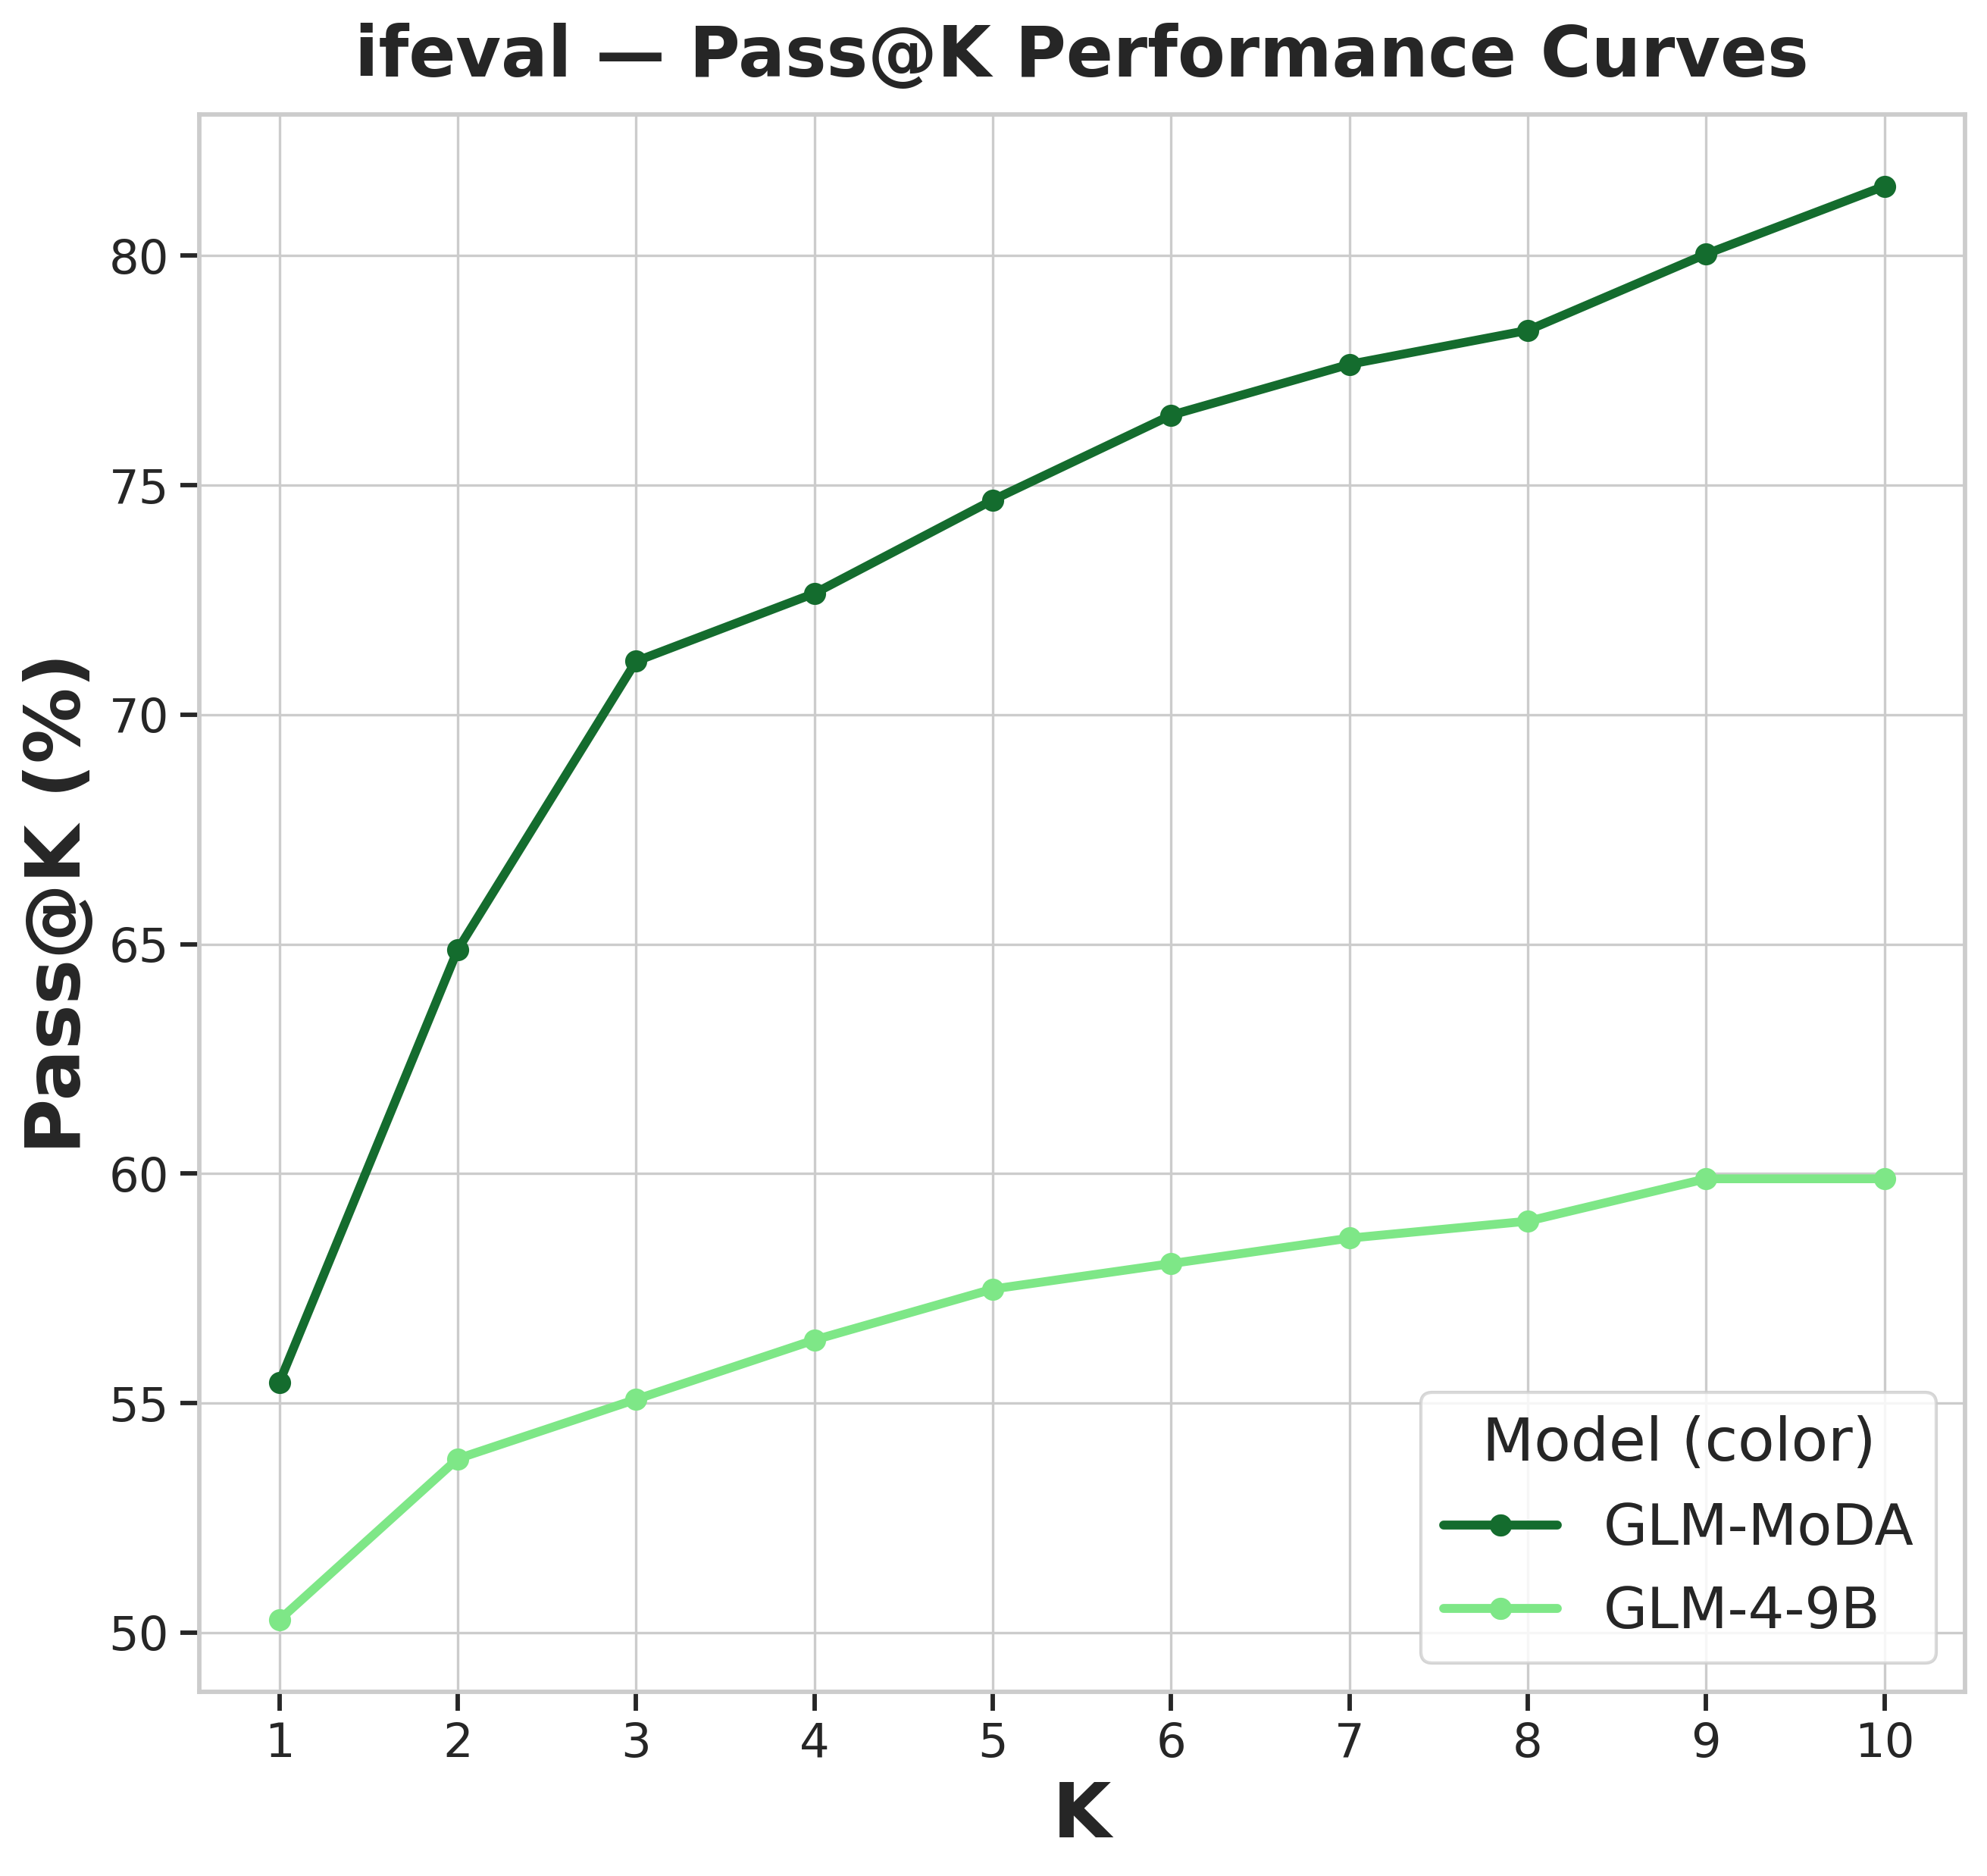
\includegraphics[width=\linewidth]{figures/main_pass_k/pass_at_k_figures/pass_at_k_ifeval_thinking_false_base_model_glm-4-9b.png}
\end{minipage}
\caption{\textbf{General capability retention: pass@k accuracy.} GLM-4-9B base and thinking disabled models.}
\label{fig:general capability pass@k glm}
\end{figure}

\subsection{Ablation Results}
\label{appx: ablation results}
We show the mean benchmark accuracy, under both standard and diverse decoding mode, on the general capability suite, and Infinite-Chat response diversity on the held out test set for the ablation study models.
\begin{table}[H]
\centering
\setlength{\tabcolsep}{3pt}
\resizebox{\textwidth}{!}{%
\begin{tabular}{lccccc}
\toprule
& \multicolumn{2}{c}{General capability (Avg., \%)} & \multicolumn{3}{c}{Infinite-Chat Diversity} \\
\cmidrule(lr){2-3} \cmidrule(lr){4-6}
Ablation & Standard mode & Diverse mode & Disc. & SBERT & E-Vendi \\
\midrule
Role-conditioned prompting & 62.9  & 56.6  & 0.403  & 0.145  & 1.90  \\
Quality only & 63.2  & 61.8  & 0.401  & 0.131  & 1.82  \\
Diversity only & 61.1  & 10.7  & \textbf{0.656}  & \textbf{0.993}  & \textbf{9.77}  \\
Additive $w{=}1$ & 67.4  & 68.0  & 0.422  & 0.204  & 2.33  \\
Additive $w{=}10$ & 64.5  & 5.7  & 0.632  & 0.976  & 9.64  \\
Additive $w{=}100$ & 61.6  & 5.4  & 0.621  & 0.970  & 8.75  \\
Token-based roles & 69.7  & 67.9 & 0.419 & 0.197 & 2.04 \\
Crafted personas & 70.1  & 66.1  & 0.421  & 0.194  & 2.24  \\
Single role & 69.0  & 69.9  & 0.428  & 0.239  & 2.57  \\
\midrule
Qwen3-8B & 62.9 & - & 0.400 & 0.132 & 1.83 \\
\midrule
\textbf{\method{}} & \textbf{73.2}  & \textbf{71.6}  & 0.444  & 0.257  & 2.69  \\
\bottomrule
\end{tabular}
}
\vspace{4pt}
\caption{\textbf{Ablation results} for general capability (Pass@1) under standard and diverse decoding (accuracy \%) and Infinite-Chat diversity ($n{=}3$ random seeds). Bold marks the best value per column.}
\label{tab:ablation}
\vspace{-0.6cm}
\end{table}

\begin{figure}
\begin{minipage}{0.32\textwidth}
  \centering
  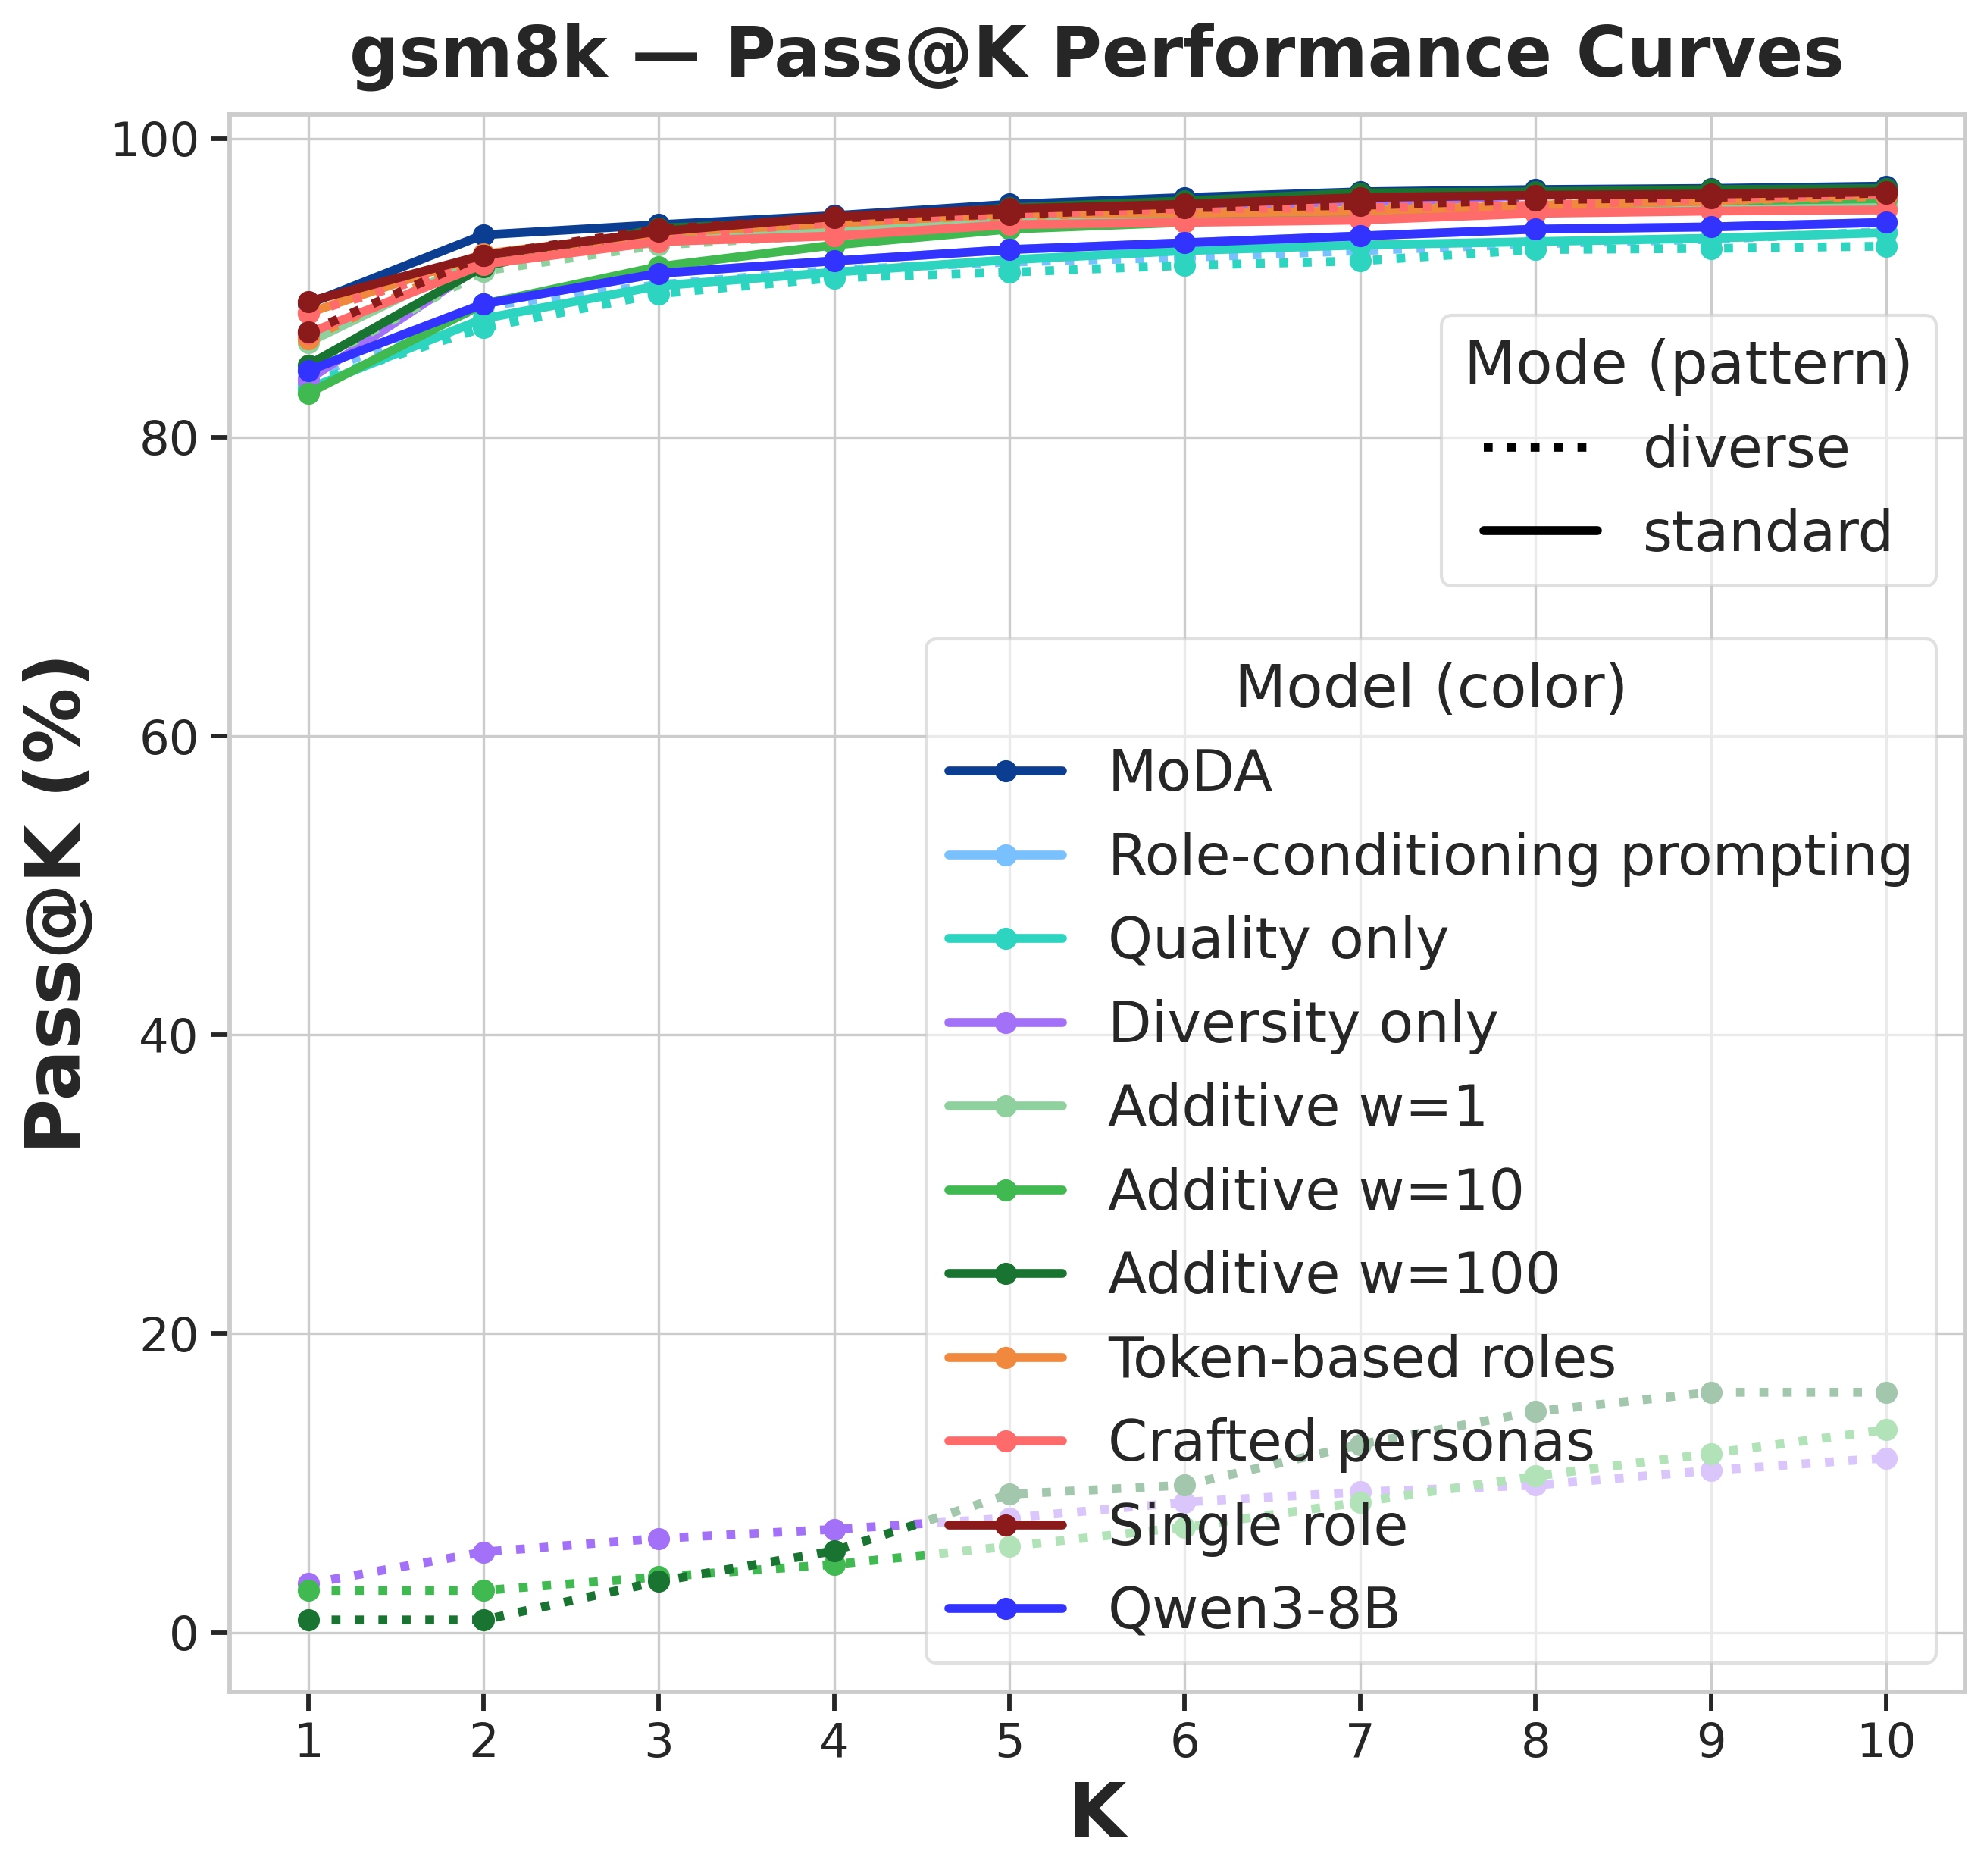
\includegraphics[width=\linewidth]{figures/ablation_pass_k/pass_at_k_gsm8k_ablations.png}
  \small Pass@k, GSM8K
  \label{fig: ablation pass@k GSM8K}
\end{minipage}\hfill
\centering
\begin{minipage}{0.32\textwidth}
  \centering
  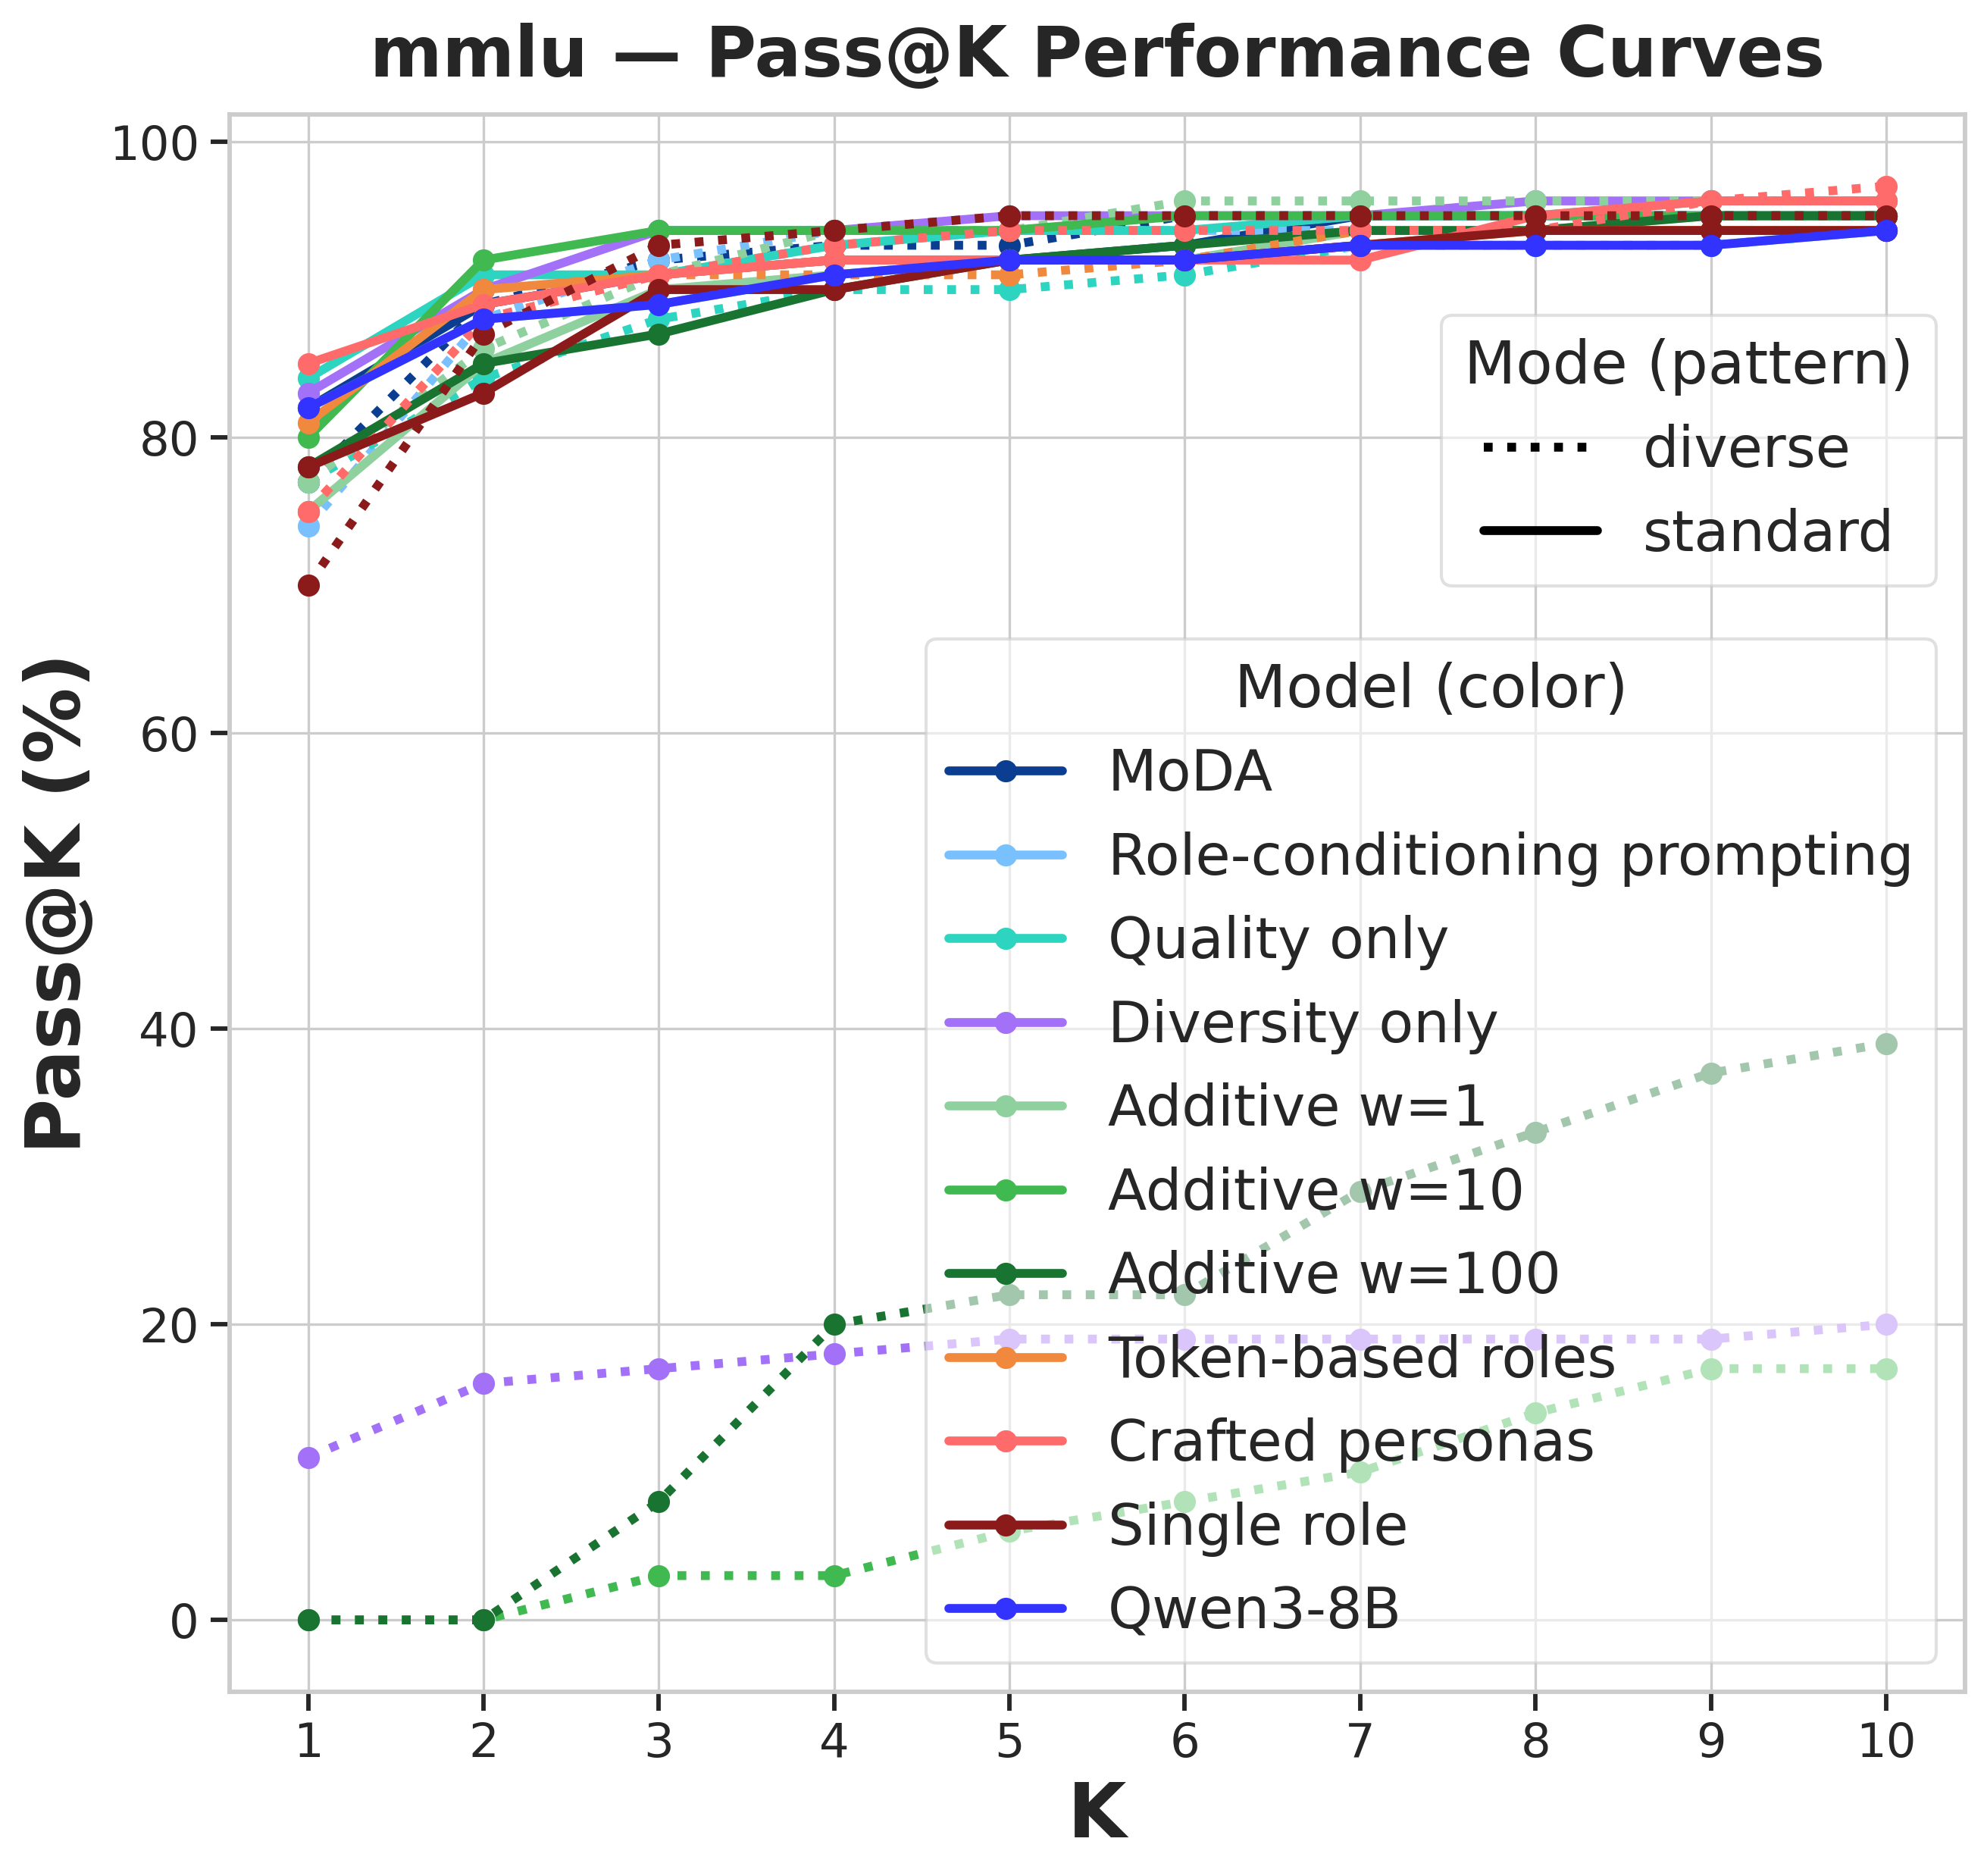
\includegraphics[width=\linewidth]{figures/ablation_pass_k/pass_at_k_mmlu_ablations.png}
  \small Pass@k, MMLU
  \label{fig: ablation pass@k MMLU}
\end{minipage}\hfill
\centering
\begin{minipage}{0.32\textwidth}
  \centering
  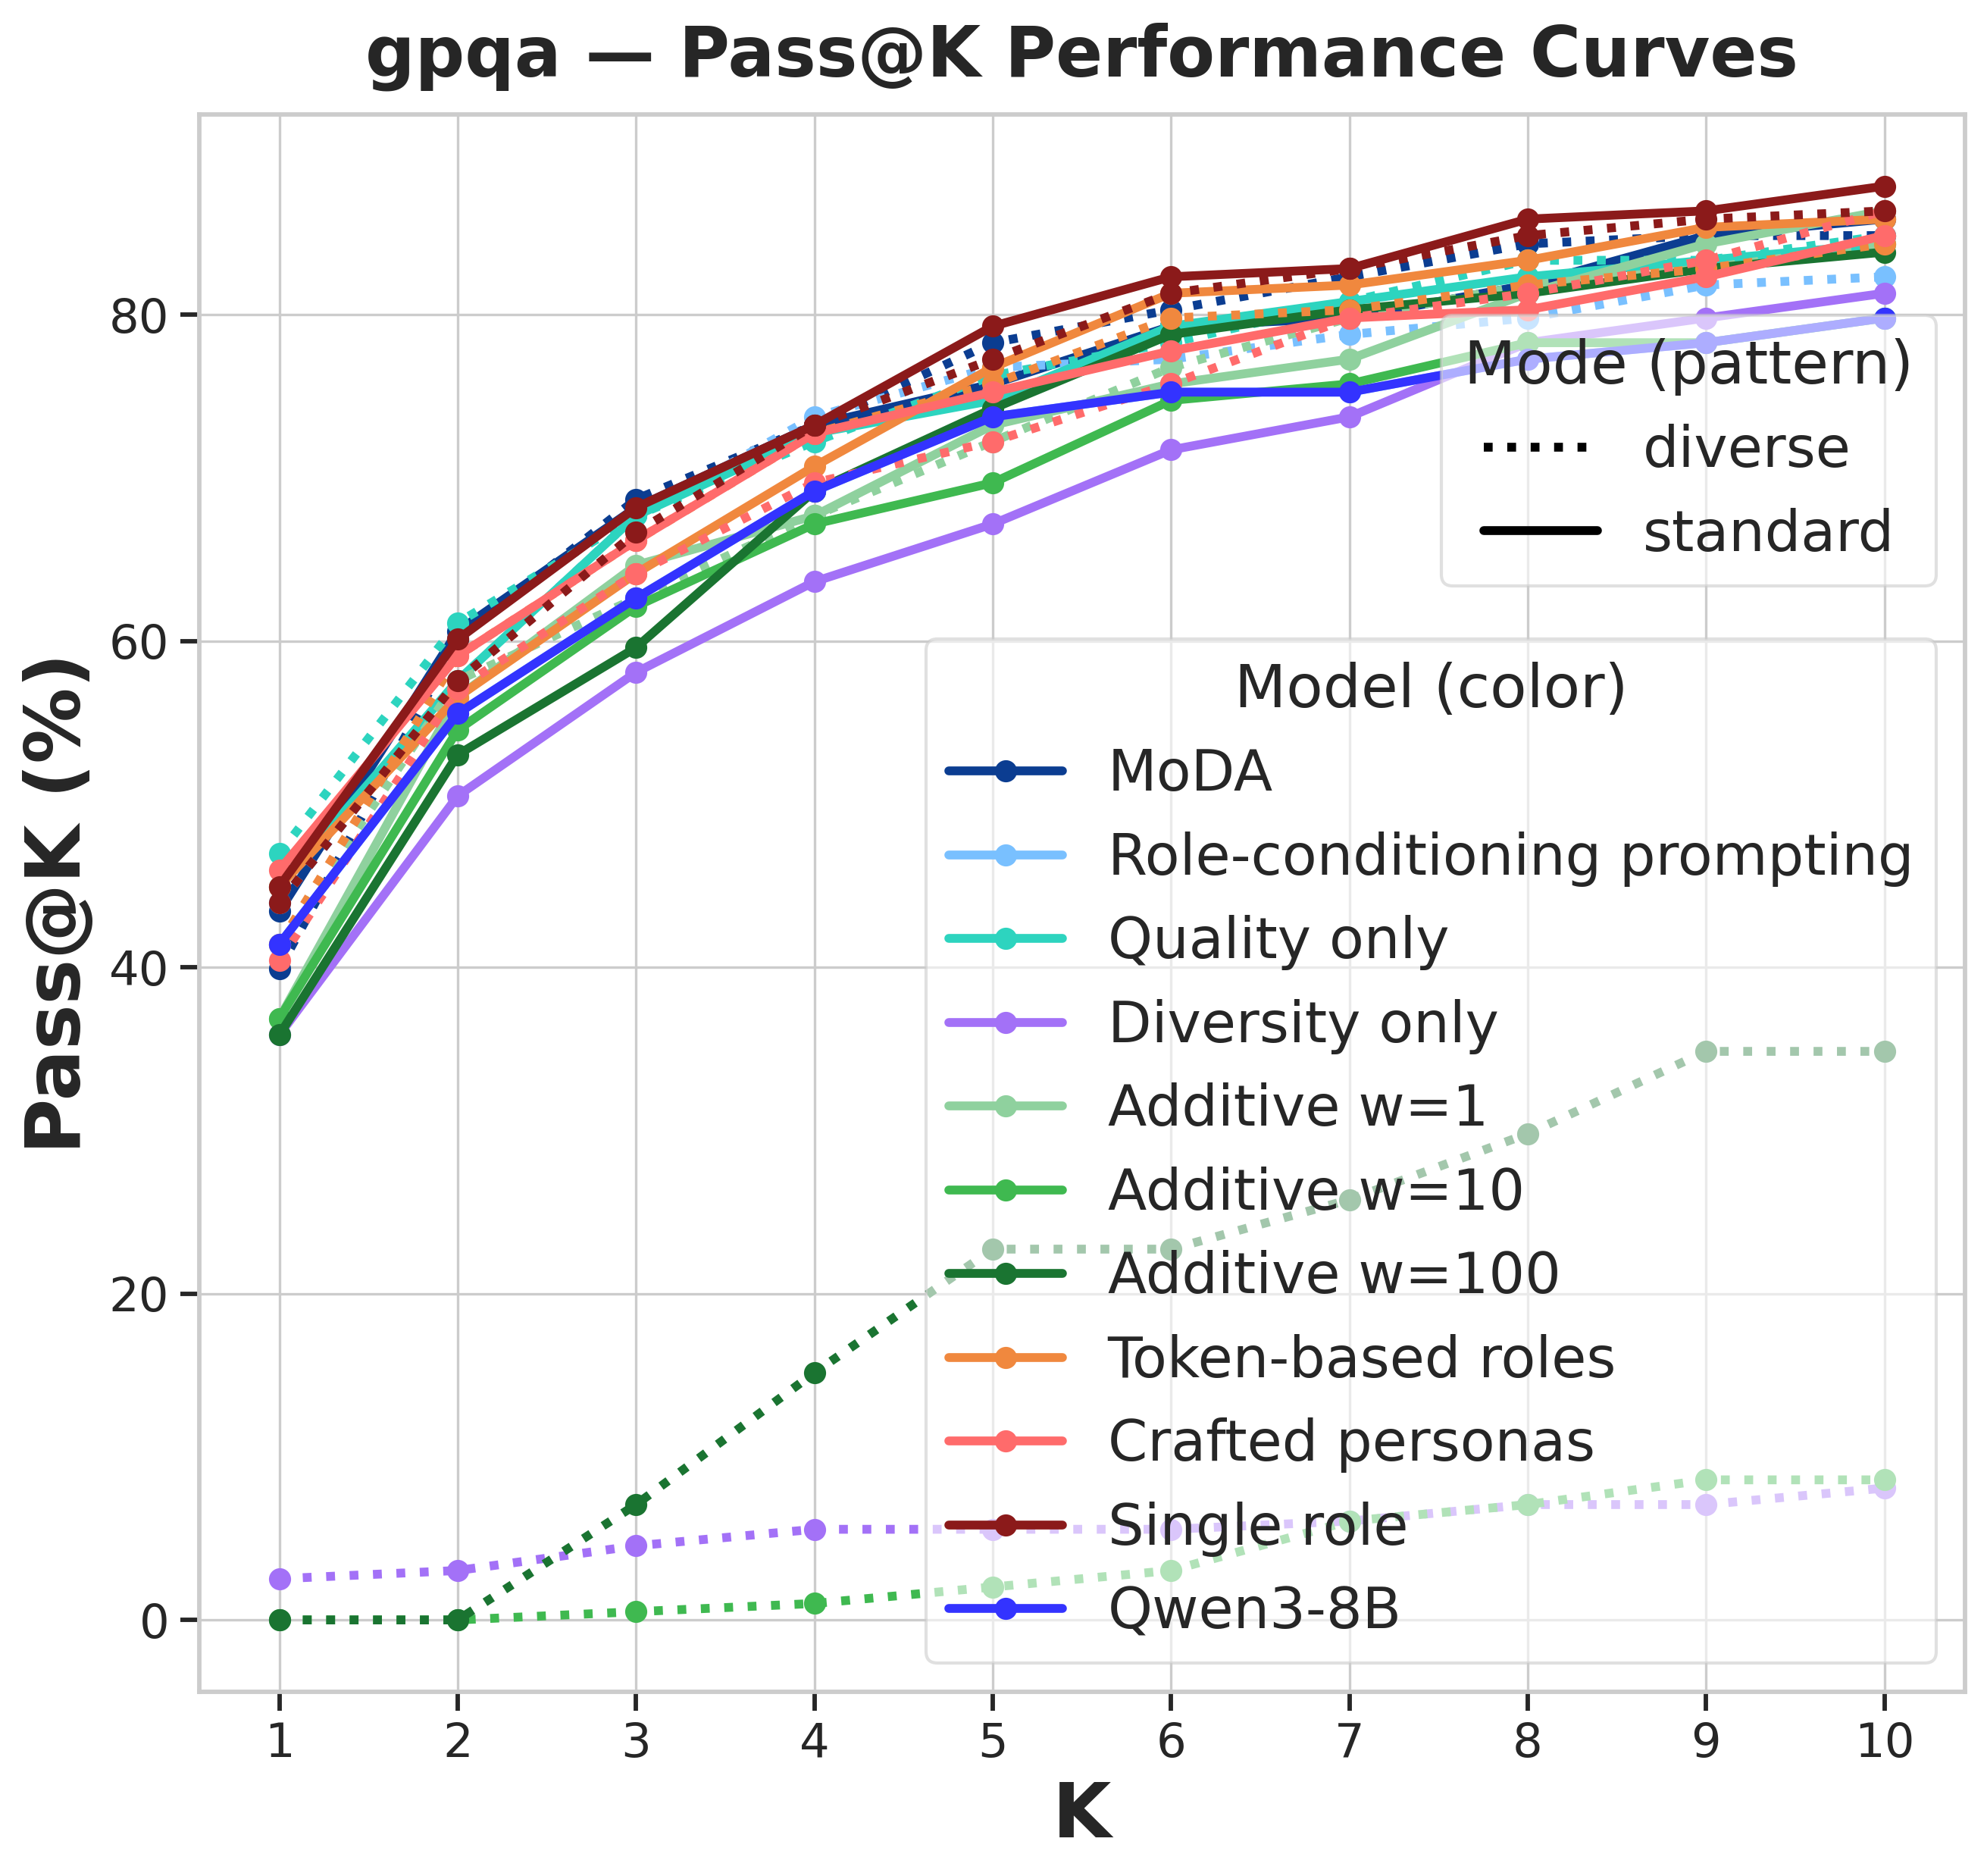
\includegraphics[width=\linewidth]{figures/ablation_pass_k/pass_at_k_gpqa_ablations.png}
  \small Pass@k, GPQA
  \label{fig: ablation pass@k GPQA}
\end{minipage}\hfill
\centering
\begin{minipage}{0.32\textwidth}
  \centering
  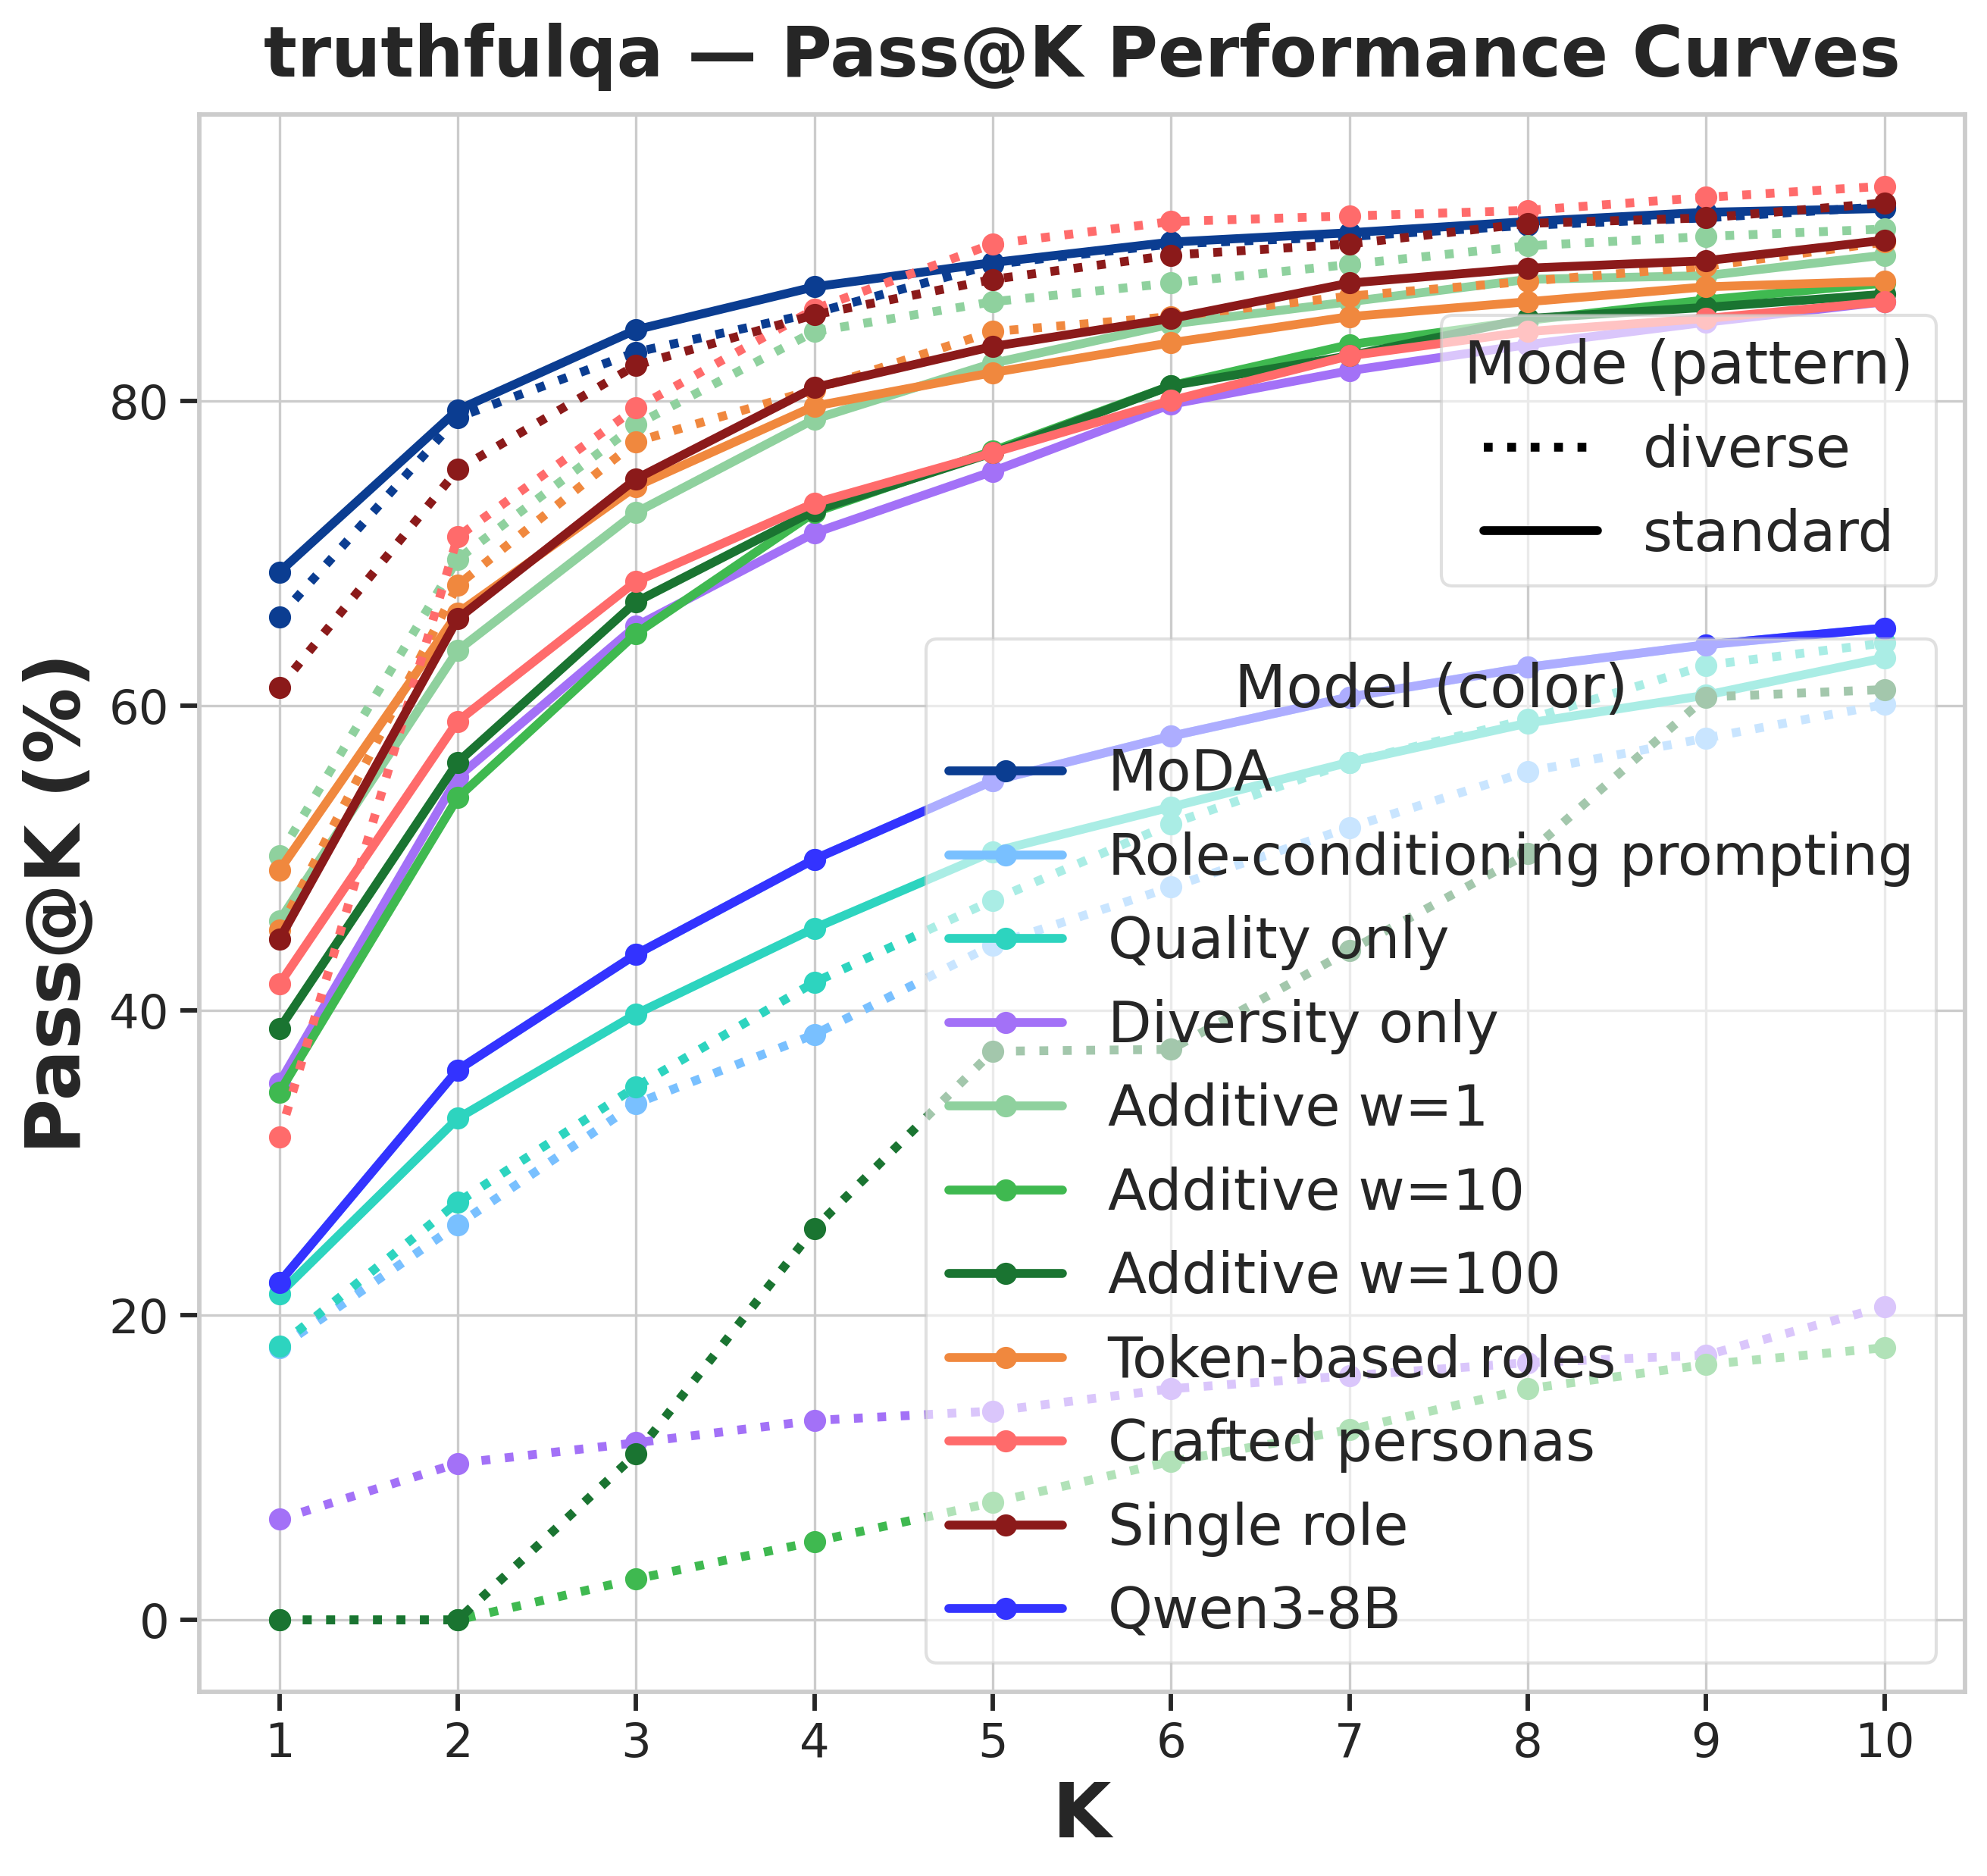
\includegraphics[width=\linewidth]{figures/ablation_pass_k/pass_at_k_truthfulqa_ablations.png}
  \small Pass@k, TruthfulQA
  \label{fig: ablation pass@k TruthfulQA}
\end{minipage}\hfill
\centering
\begin{minipage}{0.32\textwidth}
  \centering
  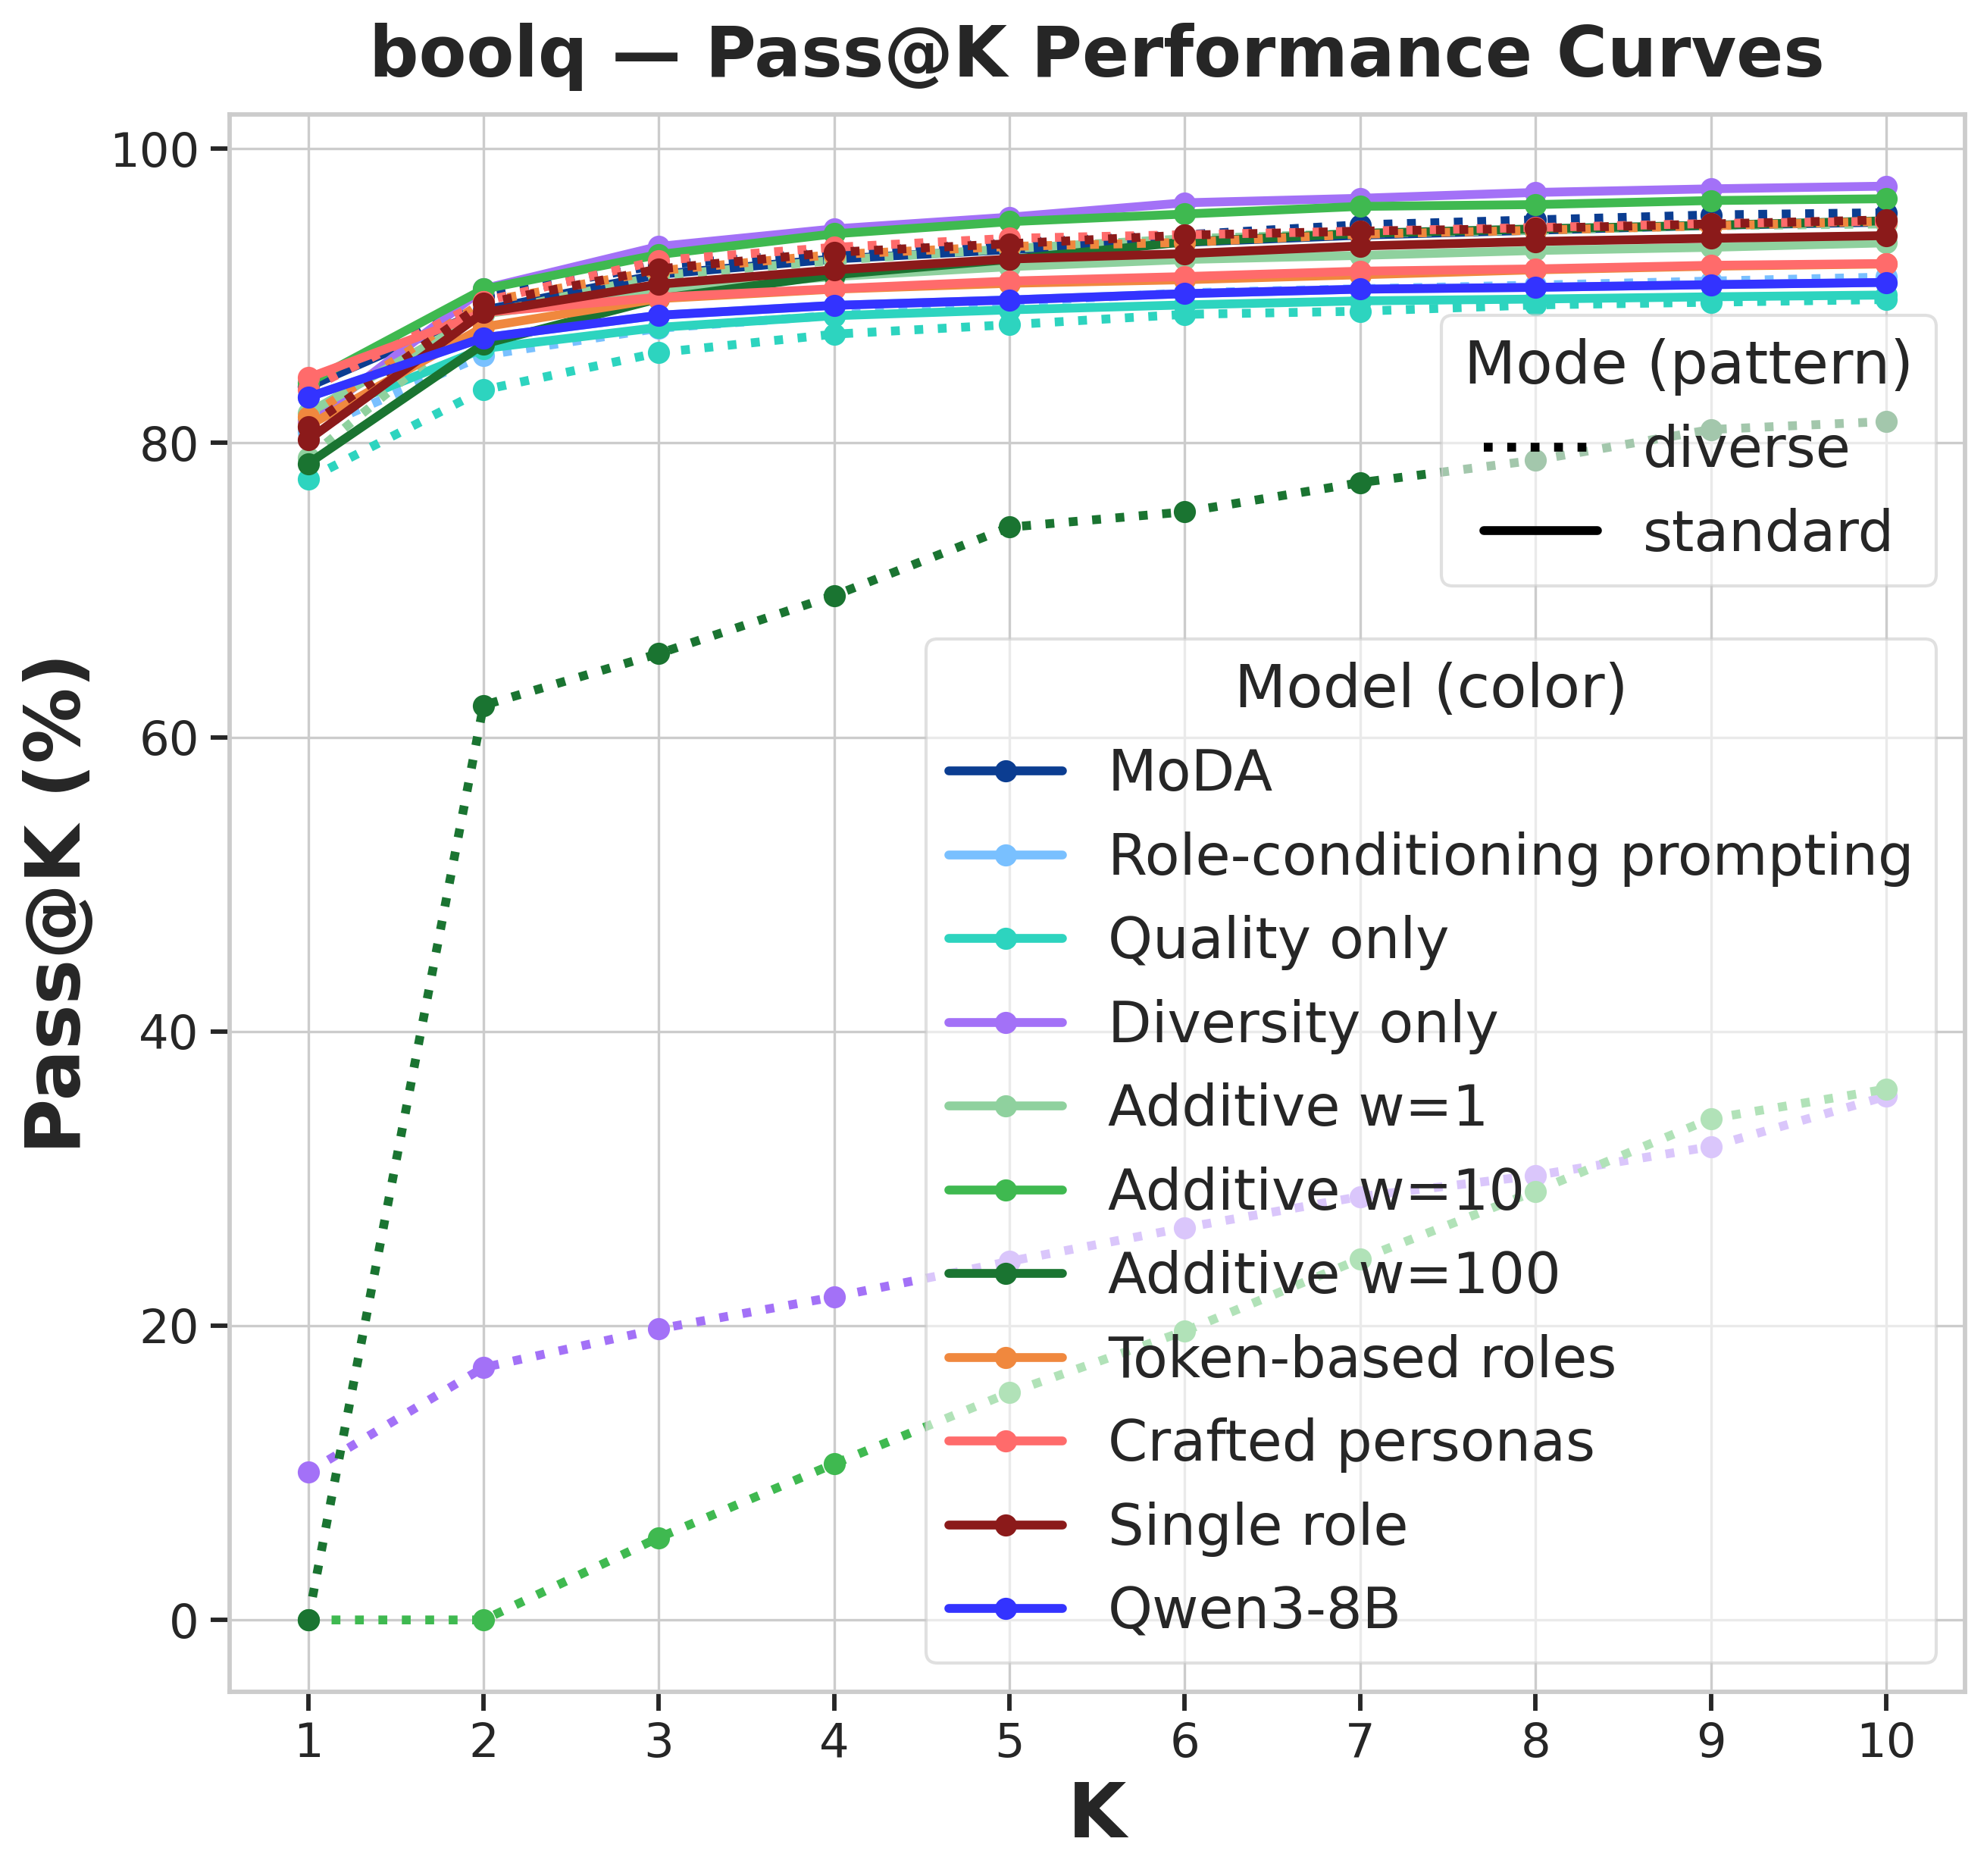
\includegraphics[width=\linewidth]{figures/ablation_pass_k/pass_at_k_boolq_ablations.png}
  \small Pass@k, BoolQ
  \label{fig: ablation pass@k BoolQ}
\end{minipage}\hfill
\centering\begin{minipage}{0.32\textwidth}
  \centering
  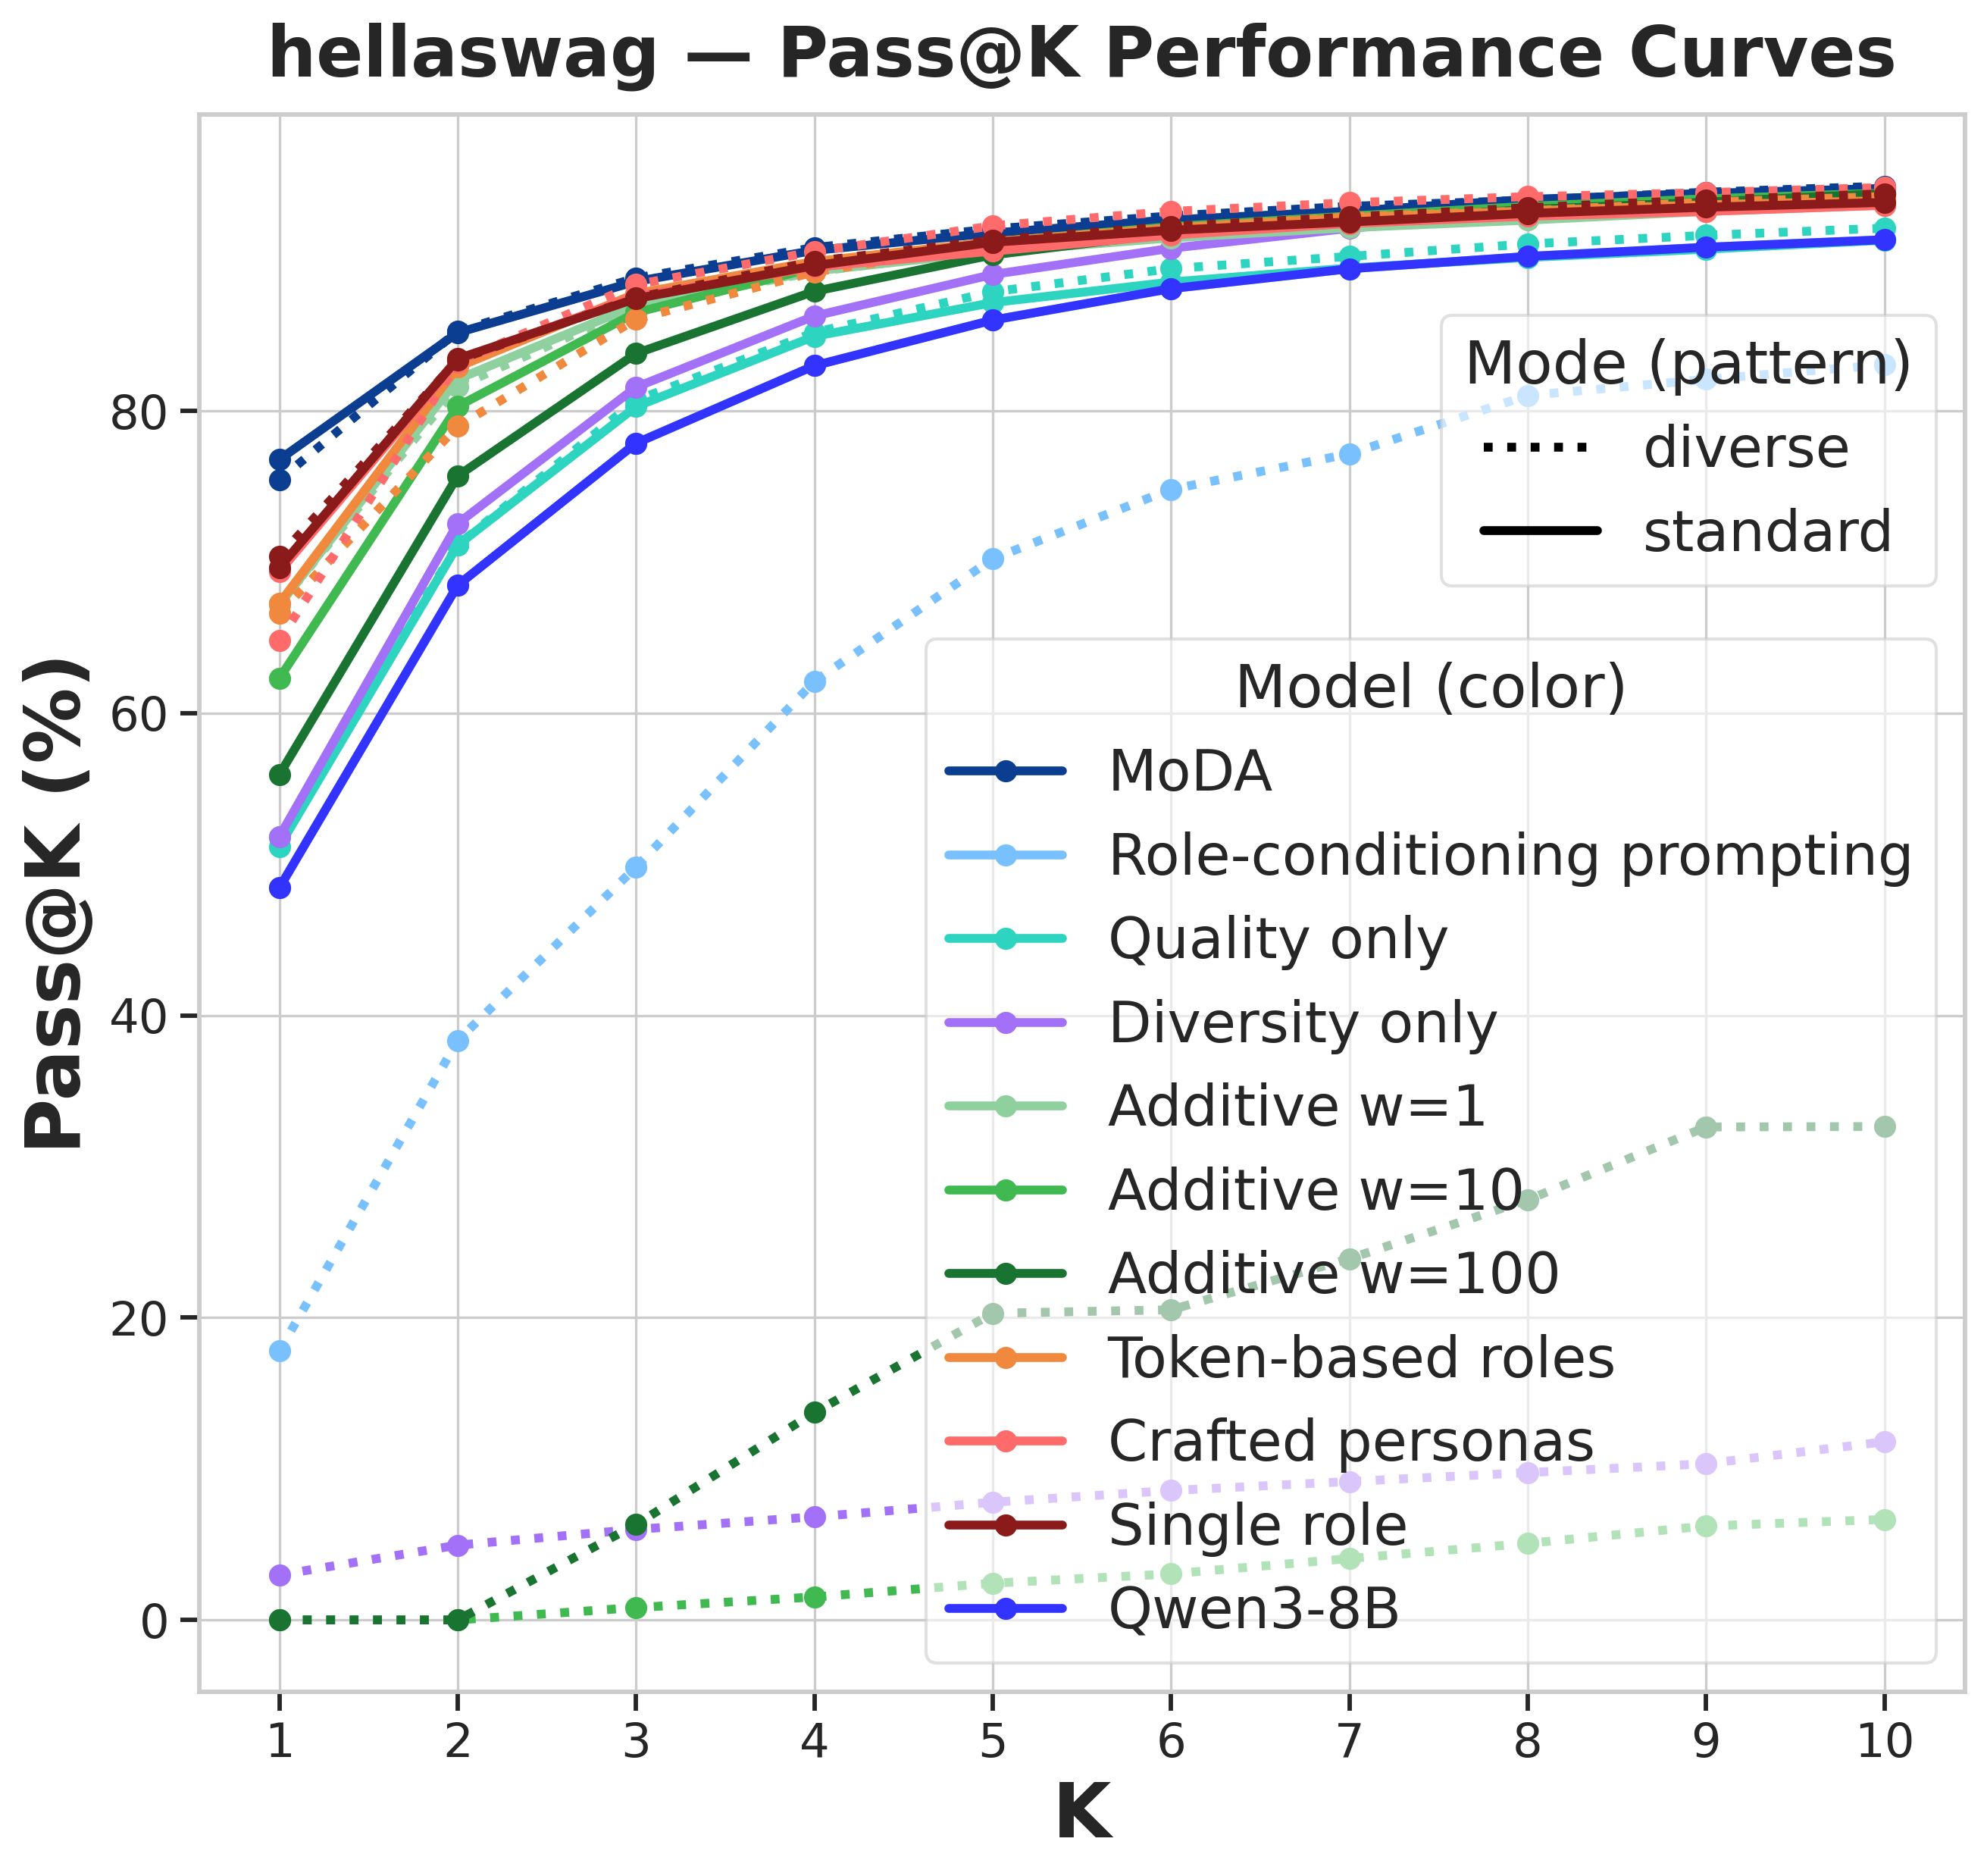
\includegraphics[width=\linewidth]{figures/ablation_pass_k/pass_at_k_hellaswag_ablations.png}
  \small Pass@k, HellaSwag
  \label{fig: ablation pass@k HellaSwag}
\end{minipage}\hfill
\centering
\begin{minipage}{0.32\textwidth}
  \centering
  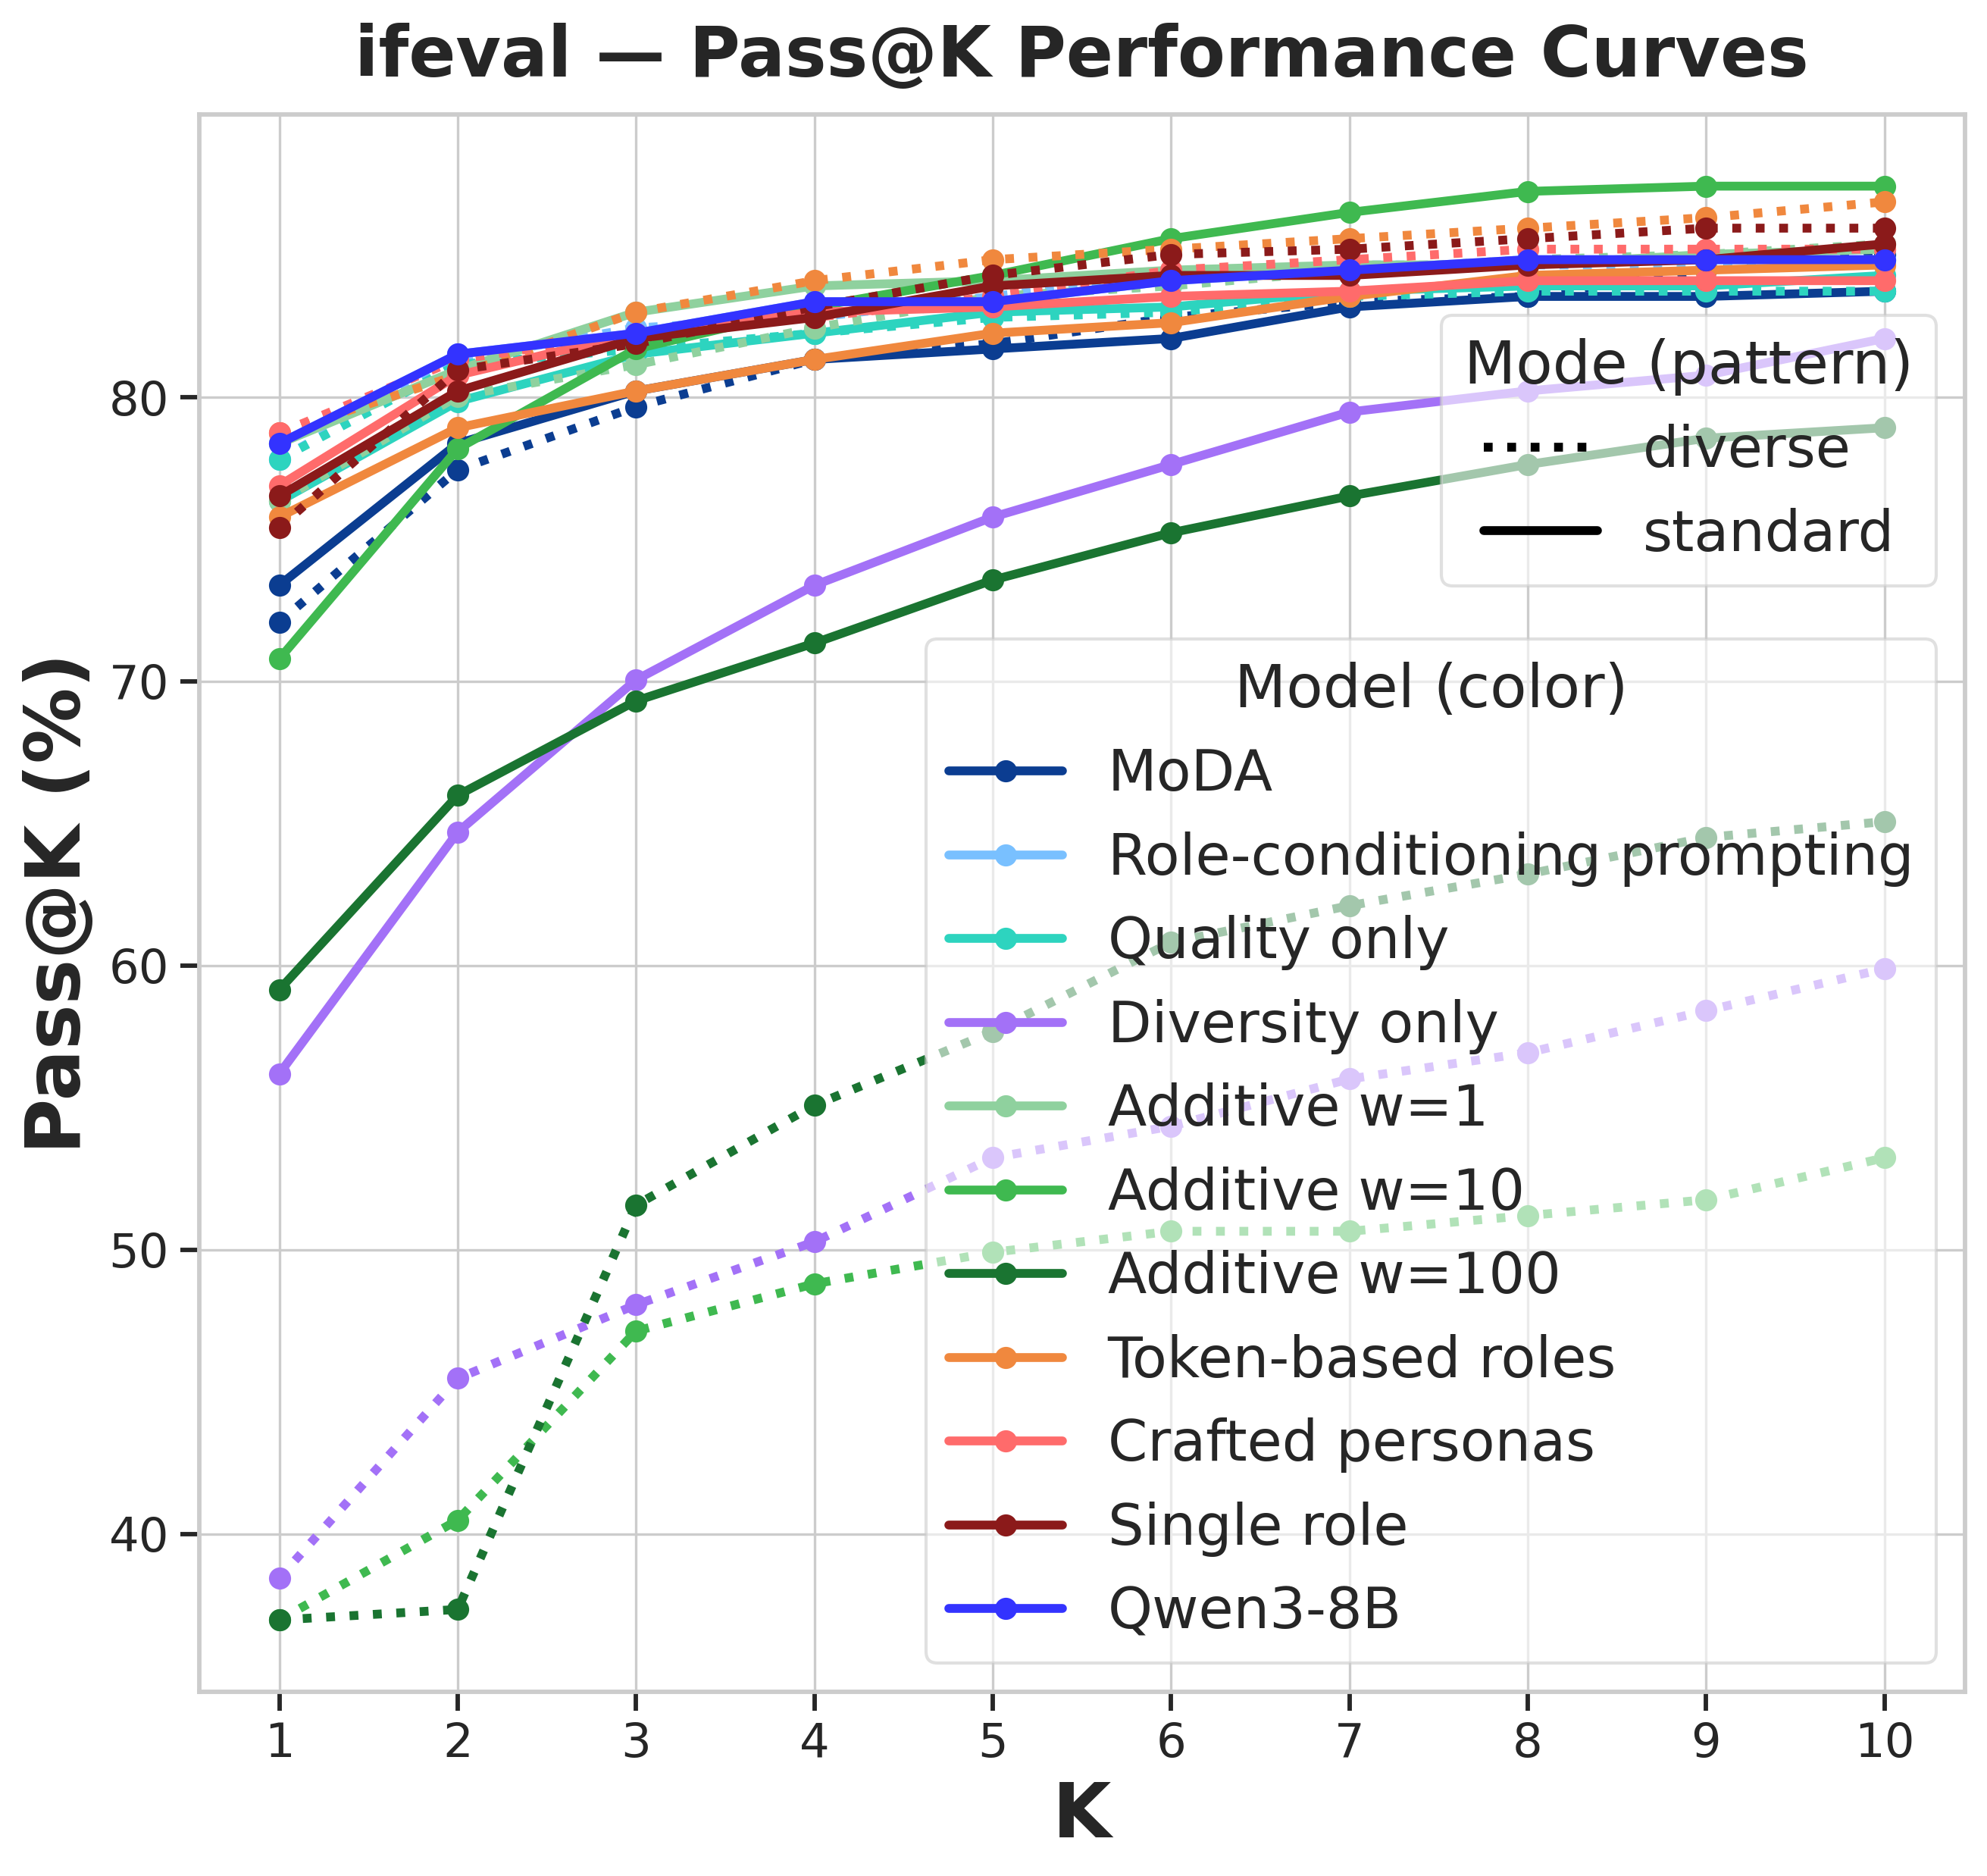
\includegraphics[width=\linewidth]{figures/ablation_pass_k/pass_at_k_ifeval_ablations.png}
  \small Pass@k, IF-Eval
  \label{fig: ablation pass@k IF-Eval}
\end{minipage}\hfill
\caption{\textbf{General capability retention for ablated models}: pass@k accuracy by benchmarks, standard vs diverse decoding mode.}
\label{fig:general capability pass@k ablation by benchmark}
\end{figure}
